\documentclass[10pt]{article}
\usepackage{tmlr}
\usepackage{amsmath,amssymb,amsthm,mathtools,booktabs,microtype,enumitem,longtable,array}
\usepackage{graphicx}
\usepackage{placeins}
\usepackage{hyperref}
\usepackage{url}
\hypersetup{hidelinks,
 pdftitle={Geometry-Induced Soft-State Abstractions for Forecasting: Supplementary Studies},
 pdfauthor={Anonymous authors},
 pdfsubject={Soft memberships, geometric enrichment, external forecasting utility, and supporting evidence}}
\newtheorem{proposition}{Proposition}
\allowdisplaybreaks
\newcommand{\R}{\mathbb{R}}
\newcommand{\E}{\mathbb{E}}
\newcommand{\Var}{\operatorname{Var}}
\newcommand{\MSE}{\operatorname{MSE}}
\newcommand{\K}{\mathrm{K}}
\newcommand{\A}{\mathrm{A}}
\newcommand{\clip}{\operatorname{clip}}
\renewcommand{\thesection}{S\arabic{section}}
\renewcommand{\theequation}{S\arabic{equation}}
\renewcommand{\thetable}{S\arabic{table}}
\renewcommand{\thefigure}{S\arabic{figure}}
\renewcommand{\theproposition}{S\arabic{proposition}}
% Generated from archived records; descriptive ratios have no ratio intervals.
\newcommand{\ConfirmationReplicates}{24}
\newcommand{\StageOneFamilySize}{29}
\newcommand{\CapacityFamilySize}{12}
\newcommand{\StageOneCriticalValue}{3.545808}
\newcommand{\CapacityCriticalValue}{3.180663}
\newcommand{\FlatWithinAffineMSE}{1.002694}
\newcommand{\FlatWithinKAHMMSE}{0.024668}
\newcommand{\FlatWithinNativeAffineMSE}{0.004641}
\newcommand{\FlatWithinRawMSE}{0.003330}
\newcommand{\FlatWithinGeometryGain}{0.978026}
\newcommand{\FlatAlignmentInteraction}{-0.978039}
\newcommand{\CurvedAlignmentInteraction}{-0.009564}
\newcommand{\VDPPhiRidgeMSE}{0.111108}
\newcommand{\VDPKAHMLocalRidgeMSE}{0.014475}
\newcommand{\VDPAffineLocalRidgeMSE}{0.011582}
\newcommand{\AirfoilRawRidgeMSE}{19.4726}
\newcommand{\AirfoilRawRBFMSE}{15.6898}
\newcommand{\AirfoilKAHMLocalRBFMSE}{20.9313}
\newcommand{\LocalPracticalBenefitCount}{8}
\newcommand{\CapacityPracticalBenefitCount}{4}
\newcommand{\VDPRawNarrowMSE}{0.002858644}
\newcommand{\VDPAffineNarrowMSE}{0.001376729}
\newcommand{\VDPKAHMNarrowMSE}{0.001026627}
\newcommand{\VDPRawNarrowRelativeGain}{64.1}
\newcommand{\VDPAffineNarrowRelativeGain}{25.4}
\newcommand{\VDPRawWideMSE}{0.001654150}
\newcommand{\VDPAffineWideMSE}{0.001078003}
\newcommand{\VDPKAHMWideMSE}{0.000871969}
\newcommand{\VDPRawWideRelativeGain}{47.3}
\newcommand{\VDPAffineWideRelativeGain}{19.1}
\newcommand{\NumericalOriginalZeroCount}{99,762}
\newcommand{\NumericalQueryClusterCount}{2,236,416}

% Generated from the unchanged confirmation method/policy reports.
\newcommand{\NaturalRawLoss}{0.8075}
\newcommand{\NaturalKAHMLoss}{0.8419}
\newcommand{\NaturalRidgeLoss}{0.7798}
\newcommand{\NaturalRawCost}{0.1688}
\newcommand{\NaturalKAHMCost}{0.3874}
\newcommand{\NaturalRidgeCost}{0.1880}
\newcommand{\NaturalErrorIncrease}{4.26}
\newcommand{\NaturalCostRatio}{2.30}
\newcommand{\NaturalProbeLoss}{0.807085}
\newcommand{\NaturalProbeCost}{0.3309}
\newcommand{\NaturalProbeCostRatio}{1.96}
\newcommand{\NaturalProbeGainPercent}{0.054}

% Generated by scaling_sensitivity/report.py from analysis/summary.json.
\newcommand{\ScalingNaturalKahmStandardLoss}{0.8419}
\newcommand{\ScalingNaturalKahmMinmaxLoss}{0.8422}
\newcommand{\ScalingNaturalRawLoss}{0.8075}
\newcommand{\ScalingNaturalRidgeLoss}{0.7798}
\newcommand{\ScalingNaturalKahmChangePercent}{0.03}
\newcommand{\ScalingNaturalKahmReductionPercent}{-0.03}
\newcommand{\ScalingNaturalKahmVsRawPercent}{4.29}
\newcommand{\ScalingNaturalKahmVsRidgePercent}{8.00}
\newcommand{\ScalingNaturalKahmStandardTime}{0.3804}
\newcommand{\ScalingNaturalKahmMinmaxTime}{0.5561}
\newcommand{\ScalingNaturalRawTime}{0.1762}
\newcommand{\ScalingNaturalRidgeTime}{0.1863}
\newcommand{\ScalingNaturalKahmCostRatioRaw}{3.16}
\newcommand{\ScalingNaturalKahmCostRatioStandard}{1.46}
\newcommand{\ScalingNaturalFamiliesImproved}{2}
\newcommand{\ScalingDevelopmentKahmStandardLoss}{2.1768}
\newcommand{\ScalingDevelopmentKahmMinmaxLoss}{2.3444}
\newcommand{\ScalingDevelopmentKahmChangePercent}{7.70}

% Generated from the fully attempted, failure-aware audited utility run.
% Archive method means without FullRoster in their name are POST-HOC common-support diagnostics.
\newcommand{\UtilityTaskCount}{168}
\newcommand{\UtilitySyntheticTasks}{144}
\newcommand{\UtilityArchiveTasks}{24}
\newcommand{\UtilityWarnings}{8}
\newcommand{\UtilityArchiveCompleteTasks}{22}
\newcommand{\UtilitySuccessfulForecasts}{1336}
\newcommand{\UtilityFailedFits}{8}
\newcommand{\UtilityFailedPolicies}{4}
\newcommand{\UtilityRawLoss}{9.1730}
\newcommand{\UtilityRawCost}{0.0037}
\newcommand{\UtilityRawCostRatio}{1.00}
\newcommand{\UtilityRawGainPercent}{0.00}
\newcommand{\UtilityRawFullRosterLoss}{9.6633}
\newcommand{\UtilityRidgeLoss}{0.8466}
\newcommand{\UtilityRidgeCost}{0.0015}
\newcommand{\UtilityRidgeCostRatio}{0.41}
\newcommand{\UtilityRidgeGainPercent}{90.77}
\newcommand{\UtilityRidgeFullRosterLoss}{1.2848}
\newcommand{\UtilityConcatLoss}{1.2111}
\newcommand{\UtilityConcatCost}{0.0691}
\newcommand{\UtilityConcatCostRatio}{18.44}
\newcommand{\UtilityConcatGainPercent}{86.80}
\newcommand{\UtilityKAHMLoss}{9.1443}
\newcommand{\UtilityKAHMCost}{0.0498}
\newcommand{\UtilityKAHMCostRatio}{13.29}
\newcommand{\UtilityKAHMGainPercent}{0.31}
\newcommand{\UtilityAffineLoss}{9.3312}
\newcommand{\UtilityAffineCost}{0.0369}
\newcommand{\UtilityAffineCostRatio}{9.83}
\newcommand{\UtilityAffineGainPercent}{-1.72}
\newcommand{\UtilityLocalityLoss}{9.5624}
\newcommand{\UtilityLocalityCost}{0.0379}
\newcommand{\UtilityLocalityCostRatio}{10.10}
\newcommand{\UtilityLocalityGainPercent}{-4.24}
\newcommand{\UtilityNaiveLoss}{1.2062}
\newcommand{\UtilityNaiveCost}{0.0012}
\newcommand{\UtilityNaiveCostRatio}{0.32}
\newcommand{\UtilityNaiveGainPercent}{86.85}
\newcommand{\UtilityNaiveFullRosterLoss}{1.5720}
\newcommand{\UtilityHGBLoss}{10.3174}
\newcommand{\UtilityHGBCost}{0.6380}
\newcommand{\UtilityHGBCostRatio}{170.20}
\newcommand{\UtilityHGBGainPercent}{-12.48}
\newcommand{\UtilityHGBFullRosterLoss}{10.7552}
\newcommand{\UtilityPolicyLoss}{9.2460}
\newcommand{\UtilityPolicyCost}{0.0467}
\newcommand{\UtilityPolicyCostRatio}{12.45}
\newcommand{\UtilityPolicyGainPercent}{-0.80}
\newcommand{\UtilityGeometryPolicyLoss}{9.2624}
\newcommand{\UtilityGeometryPolicyCost}{0.0869}
\newcommand{\UtilityGeometryPolicyCostRatio}{23.17}
\newcommand{\UtilityGeometryPolicyGainPercent}{-0.97}
\newcommand{\UtilityRawPositiveContrasts}{5}
\newcommand{\UtilityRawNegativeContrasts}{0}
\newcommand{\UtilityRawUnresolvedContrasts}{7}
\newcommand{\UtilityConcatPositiveContrasts}{6}
\newcommand{\UtilityConcatNegativeContrasts}{4}
\newcommand{\UtilityConcatUnresolvedContrasts}{2}
\newcommand{\UtilityKAHMAdoptions}{7}
\newcommand{\UtilityGeometryAdoptions}{12}
\newcommand{\UtilityArchiveKAHMNonzero}{9}
\newcommand{\UtilitySyntheticKAHMNonzero}{134}

% Generated target-geometry numbers; change is signed, negative favorable.
\newcommand{\TGTaskCount}{48}
\newcommand{\TGCompletedTaskCount}{48}
\newcommand{\TGForecastCount}{768}
\newcommand{\TGMethodCount}{16}
\newcommand{\TGFallbackCount}{0}
\newcommand{\TGPrimaryPositive}{3}
\newcommand{\TGPrimaryNegative}{5}
\newcommand{\TGPrimaryUnresolved}{10}
\newcommand{\TGNaturalLearnedMSE}{1.2721}
\newcommand{\TGNaturalRidgeMSE}{1.3005}
\newcommand{\TGNaturalChangePercent}{-2.18}
\newcommand{\TGNaturalCostRatio}{124.9}

% Generated from the preserved direct-reconstruction summary; no manual numerical edits.
\newcommand{\DirectPlannedTasks}{46}
\newcommand{\DirectAvailableTasks}{43}
\newcommand{\DirectAvailableOutputs}{731}
\newcommand{\DirectPlannedOutputs}{782}
\newcommand{\DirectUnavailableTasks}{3}
\newcommand{\DirectNaturalAvailableCollections}{3}
\newcommand{\DirectNaturalAvailableSeries}{7}
\newcommand{\DirectPrimaryPositive}{2}
\newcommand{\DirectPrimaryNegative}{6}
\newcommand{\DirectPrimaryUnresolved}{10}
\newcommand{\DirectOptimizations}{3096}
\newcommand{\DirectObjectiveEvaluations}{406832}
\newcommand{\DirectFallbackEvents}{0}

\newcommand{\PPTasks}{192}
\newcommand{\PPRepetitions}{24}
\newcommand{\PPHistory}{12}
\newcommand{\PPOrigins}{13}
\newcommand{\PPPrimaryCount}{4}
\newcommand{\PPPrimaryEstablished}{1}
\newcommand{\PPArraysPerTask}{502}
\newcommand{\PPTotalArrays}{96,384}
\newcommand{\PPEpisodesA}{64}
\newcommand{\PPEpisodesB}{32}
\newcommand{\PPEpisodesC}{32}
\newcommand{\PPEpisodesD}{128}
\newcommand{\PPRowsA}{512}
\newcommand{\PPRowsB}{256}
\newcommand{\PPRowsC}{256}
\newcommand{\PPRowsD}{1,664}
\newcommand{\PPMaxErrorRatio}{1.3762}
\newcommand{\PPPolicyPenalty}{4.02}
\newcommand{\PPRBFPenalty}{0.28}
\newcommand{\PPTanhPenalty}{6.49}
\newcommand{\PPLinearPenalty}{0.18}
\newcommand{\PPNonlinearLoss}{0.028372}
\newcommand{\PPFixedBiasGainMin}{10.78}
\newcommand{\PPFixedBiasGainMax}{14.93}
\newcommand{\PPFixedRBFGainMin}{2.37}
\newcommand{\PPFixedRBFGainMax}{4.14}
\newcommand{\PPAuditAssertions}{1,284,715}
\newcommand{\PPAuditBases}{48,384}
\newcommand{\PPAuditRawTasks}{8}
\newcommand{\PPAuditRawArrays}{4,016}
\newcommand{\PPAuditLossRows}{96,384}

\newcommand{\CFRTasks}{192}
\newcommand{\CFRRepetitions}{24}
\newcommand{\CFRHistory}{12}
\newcommand{\CFROrigins}{13}
\newcommand{\CFRPrimaryCount}{4}
\newcommand{\CFRPrimaryEstablished}{2}
\newcommand{\CFRArraysPerTask}{42}
\newcommand{\CFRTotalArrays}{8,064}
\newcommand{\CFREpisodesA}{64}
\newcommand{\CFREpisodesB}{32}
\newcommand{\CFREpisodesC}{32}
\newcommand{\CFREpisodesD}{128}
\newcommand{\CFRRowsA}{512}
\newcommand{\CFRRowsB}{256}
\newcommand{\CFRRowsC}{256}
\newcommand{\CFRRowsD}{1,664}
\newcommand{\CFRMaxErrorRatio}{1.8873}
\newcommand{\CFRGainBias}{9.20}
\newcommand{\CFRGainRBF}{2.87}
\newcommand{\CFRPolicyPenalty}{5.12}
\newcommand{\CFRLinearPenalty}{1.13}
\newcommand{\CFRISGainBias}{12.43}
\newcommand{\CFRISGainRBF}{3.96}
\newcommand{\CFROOFvsISPenalty}{3.69}
\newcommand{\CFRMatchedRBFGain}{4.17}
\newcommand{\CFRFullCommonGain}{7.72}
\newcommand{\CFRCalibrationGain}{0.69}
\newcommand{\CFROOFvsISDifference}{0.001016}
\newcommand{\CFROOFvsISLower}{0.000878}
\newcommand{\CFROOFvsISUpper}{0.001154}
\newcommand{\CFRISWinningRepetitions}{24}
\newcommand{\CFRISLoss}{0.027559}
\newcommand{\CFRISPolicyPenalty}{1.39}
\newcommand{\CFRKAHMTanhSelections}{33}
\newcommand{\CFRKAHMEtaZero}{233}
\newcommand{\CFRCalibrationCells}{576}
\newcommand{\CFRAuditAssertions}{946,138}
\newcommand{\CFRAuditBases}{21,770}
\newcommand{\CFRAuditArrays}{8,064}
\newcommand{\CFRZeroRanks}{2}
\newcommand{\CFRSVDRecoveries}{4}
\newcommand{\CFRSVDFailures}{0}
\newcommand{\CFRRecoveryTasks}{3}
\newcommand{\CFRAdditionalRepetitions}{0}

% Generated from pinned published records.
\newcommand{\PAGainPZero}{0.82}
\newcommand{\PAGainExtra}{0.66}
\newcommand{\PANaturalPenalty}{2.27}
\newcommand{\PANaturalGainExtra}{2.72}
\newcommand{\PAMechanismBiasGain}{12.50}
\newcommand{\PAMechanismRBFGain}{3.83}
\newcommand{\PAStandalonePolicyPenalty}{1.32}
\newcommand{\PASyntheticSelections}{44}
\newcommand{\PANaturalSelections}{3}
\newcommand{\PARepetitions}{24}
\newcommand{\PATasks}{192}
\newcommand{\PANaturalSeries}{48}
\newcommand{\PANaturalBiasGain}{3.33}
\newcommand{\PANaturalRBFGain}{2.15}

% Generated from completed, independently audited evidence; do not edit.
\newcommand{\SARepetitions}{32}
\newcommand{\SATasks}{256}
\newcommand{\SAFamilySize}{4}
\newcommand{\SACriteriaEstablished}{3}
\newcommand{\SACriticalT}{2.355568}
\newcommand{\SASolverRecoveries}{0}
\newcommand{\SAAuditChecks}{2563814}
\newcommand{\SAGainPG}{69.20}
\newcommand{\SAGapPG}{\ensuremath{-0.0654535}}
\newcommand{\SAUpperPG}{\ensuremath{-0.0625338}}
\newcommand{\SAEstablishedPG}{Yes}
\newcommand{\SAGainKP}{10.46}
\newcommand{\SAGapKP}{\ensuremath{-0.00227118}}
\newcommand{\SAUpperKP}{\ensuremath{-0.00198733}}
\newcommand{\SAEstablishedKP}{Yes}
\newcommand{\SAGainKR}{0.03}
\newcommand{\SAGapKR}{0.000810251}
\newcommand{\SAUpperKR}{0.000981018}
\newcommand{\SAEstablishedKR}{No}
\newcommand{\SAGainLinearKP}{\ensuremath{-1.11}}
\newcommand{\SAGapLinearKP}{\ensuremath{-0.0354224}}
\newcommand{\SAUpperLinearKP}{\ensuremath{-0.031341}}
\newcommand{\SAEstablishedLinearKP}{Yes}
\newcommand{\SALossSharedNonlinearG}{0.0988703}
\newcommand{\SALossSharedNonlinearP}{0.0304507}
\newcommand{\SALossSharedNonlinearK}{0.027266}
\newcommand{\SALossSharedNonlinearR}{0.027274}
\newcommand{\SALossSharedLinearG}{0.939042}
\newcommand{\SALossSharedLinearP}{0.910921}
\newcommand{\SALossSharedLinearK}{0.921045}
\newcommand{\SALossSharedLinearR}{0.915866}
\newcommand{\SALossIndependentNonlinearG}{0.0988703}
\newcommand{\SALossIndependentNonlinearP}{0.0304507}
\newcommand{\SALossIndependentNonlinearK}{0.0267546}
\newcommand{\SALossIndependentNonlinearR}{0.0267507}
\newcommand{\SALossIndependentLinearG}{0.939042}
\newcommand{\SALossIndependentLinearP}{0.910921}
\newcommand{\SALossIndependentLinearK}{0.914936}
\newcommand{\SALossIndependentLinearR}{0.91589}
\newcommand{\SAFitWallHours}{0.26}
\newcommand{\SAFitCPUHours}{0.26}
\newcommand{\SAPredictionWallSeconds}{671.84}
\newcommand{\SAPeakWorkerRSSMiB}{156.99}
\newcommand{\SAStateNPZMiB}{177.93}

% Generated from completed, independently audited joint-selection evidence.
\newcommand{\JSRepetitions}{32}
\newcommand{\JSTasks}{256}
\newcommand{\JSCandidates}{15}
\newcommand{\JSScalings}{3}
\newcommand{\JSCaps}{5}
\newcommand{\JSFamilySize}{6}
\newcommand{\JSCriteriaEstablished}{4}
\newcommand{\JSAuditChecks}{7{,}422{,}883}
\newcommand{\JSSolverRecoveries}{0}
\newcommand{\JSCriticalT}{2.530926}
\newcommand{\JSGainPG}{68.69}
\newcommand{\JSRelativeLossChangePG}{-68.69}
\newcommand{\JSGapPG}{-0.0616038}
\newcommand{\JSUpperPG}{-0.0587852}
\newcommand{\JSEstablishedPG}{Yes}
\newcommand{\JSGainKP}{8.86}
\newcommand{\JSRelativeLossChangeKP}{-8.86}
\newcommand{\JSGapKP}{-0.00171995}
\newcommand{\JSUpperKP}{-0.00144862}
\newcommand{\JSEstablishedKP}{Yes}
\newcommand{\JSGainKR}{-0.9186}
\newcommand{\JSRelativeLossChangeKR}{0.9186}
\newcommand{\JSGapKR}{0.00103904}
\newcommand{\JSUpperKR}{0.00119423}
\newcommand{\JSEstablishedKR}{No}
\newcommand{\JSGainLinearKP}{-1.26}
\newcommand{\JSRelativeLossChangeLinearKP}{1.26}
\newcommand{\JSGapLinearKP}{-0.0342551}
\newcommand{\JSUpperLinearKP}{-0.0305374}
\newcommand{\JSEstablishedLinearKP}{Yes}
\newcommand{\JSGainJointKNonlinear}{0.0727}
\newcommand{\JSRelativeLossChangeJointKNonlinear}{-0.0727}
\newcommand{\JSGapJointKNonlinear}{0.00076781}
\newcommand{\JSUpperJointKNonlinear}{0.000901116}
\newcommand{\JSEstablishedJointKNonlinear}{No}
\newcommand{\JSGainJointKLinear}{-0.2491}
\newcommand{\JSRelativeLossChangeJointKLinear}{0.2491}
\newcommand{\JSGapJointKLinear}{-0.0436414}
\newcommand{\JSUpperJointKLinear}{-0.0417521}
\newcommand{\JSEstablishedJointKLinear}{Yes}
\newcommand{\JSLossSharedNonlinearG}{0.0937767}
\newcommand{\JSLossSharedLinearG}{0.940694}
\newcommand{\JSLossSharedNonlinearP}{0.0293596}
\newcommand{\JSLossSharedLinearP}{0.915564}
\newcommand{\JSLossSharedNonlinearK}{0.0267588}
\newcommand{\JSLossSharedLinearK}{0.927087}
\newcommand{\JSLossSharedNonlinearR}{0.0265152}
\newcommand{\JSLossSharedLinearR}{0.919841}
\newcommand{\JSLossIndependentNonlinearG}{0.0921642}
\newcommand{\JSLossIndependentLinearG}{0.937323}
\newcommand{\JSLossIndependentNonlinearP}{0.0293596}
\newcommand{\JSLossIndependentLinearP}{0.915564}
\newcommand{\JSLossIndependentNonlinearK}{0.0262103}
\newcommand{\JSLossIndependentLinearK}{0.920881}
\newcommand{\JSLossIndependentNonlinearR}{0.0259918}
\newcommand{\JSLossIndependentLinearR}{0.920442}
\newcommand{\JSLossStandardSharedNonlinearG}{0.0966196}
\newcommand{\JSLossStandardSharedLinearG}{0.943965}
\newcommand{\JSLossStandardSharedNonlinearP}{0.029789}
\newcommand{\JSLossStandardSharedLinearP}{0.914789}
\newcommand{\JSLossStandardSharedNonlinearK}{0.0266938}
\newcommand{\JSLossStandardSharedLinearK}{0.922462}
\newcommand{\JSLossStandardSharedNonlinearR}{0.0266479}
\newcommand{\JSLossStandardSharedLinearR}{0.919456}
\newcommand{\JSLossStandardIndependentNonlinearG}{0.0966196}
\newcommand{\JSLossStandardIndependentLinearG}{0.943965}
\newcommand{\JSLossStandardIndependentNonlinearP}{0.029789}
\newcommand{\JSLossStandardIndependentLinearP}{0.914789}
\newcommand{\JSLossStandardIndependentNonlinearK}{0.0262294}
\newcommand{\JSLossStandardIndependentLinearK}{0.918593}
\newcommand{\JSLossStandardIndependentNonlinearR}{0.0260926}
\newcommand{\JSLossStandardIndependentLinearR}{0.918714}
\newcommand{\JSFitCpuMinutes}{19.63}
\newcommand{\JSFitWallSumMinutes}{19.63}
\newcommand{\JSFitMedianSeconds}{4.56}
\newcommand{\JSQueryWallSumMinutes}{12.67}

\title{Geometry-Induced Soft-State Abstractions\\
for Forecasting:\\Supplementary Studies}
\author{Anonymous authors}
\begin{document}
\maketitle
\begin{abstract}
This document presents supporting theory and experiments on predictive
enrichment of geometry-induced soft-state abstractions with Kernel Affine
Hull Machines. The main representation combines partitionwise soft
memberships with local coordinates and reconstruction departures; only
the membership block takes values in a product of simplices. The
supporting studies also evaluate distinct discrepancy codes, raw-history
augmentations, and learned or adaptive geometric encodings, each with
its own definition and decoder. Direct forecasts of observed future
outputs assess external predictive utility without testing linear
propagation of the soft coordinates or Koopman closure.
The document establishes the supporting information and residual-risk
identities, and specifies the controlled, natural-data, scaling, additive,
metric-learning, reconstruction-training, and online-adaptation experiments.
Two later studies evaluate preprocessing with native dimension selection
and centered departure corrections around fixed common forecasts. The
residual-target study is reported through a computational reproduction
of its prescribed cohort, with no added independent repetitions.
A subsequent policy-augmentation study evaluates a centered in-sample
KAHM correction on fresh simulation repetitions and a separate
48-series chronological M4 training-data panel. It does not establish
either prespecified nonlinear policy advantage, and its natural-series
results remain descriptive benchmark-development evidence.
Complete comparison families, source-level results, resource measurements,
and unsuccessful or unavailable configurations accompany their protocols.
The studies use different procedures and evaluation populations. Their
results are interpreted separately from one another and from the
earlier dimension-selected experiment in the accompanying main paper.
The preceding \SARepetitions-repetition representation-only study compares
memberships, local position, KAHM enrichment and matched RBF enrichment
on \SATasks\ task suites. Its single four-contrast primary family
establishes the nonlinear position and KAHM-enrichment margins and
linear noninferiority, but not the prescribed KAHM-over-RBF superiority
margin. Complete primary results, descriptive decompositions and
independent computational audit coverage accompany the frozen protocol.
A separately frozen joint scaling--dimension study adds \JSRepetitions\
fresh repetitions and \JSTasks\ tasks. Its six-contrast family establishes
the nonlinear position and KAHM-enrichment margins and both linear
noninferiority criteria. Neither KAHM-over-RBF superiority nor a 3\%
benefit from expanding KAHM's scaling menu is established. The latter
comparison uses dimension-selected standard-only candidates from the
same cohort; its nonlinear point gain is \JSGainJointKNonlinear\%.
Complete forecast means, scaler and cap choices, law-level results,
and numerical verification records accompany the joint-selection design.
\end{abstract}

\section{Scope, evidence, and notation}\label{supp:scope}
The supporting experiments examine how geometric state descriptions and
their enrichment affect fitted forecasts of a specified response.\footnote{AI tools assisted with
protocol development, implementation, numerical and statistical
verification, analysis, and manuscript preparation. The authors are
responsible for the scientific claims, evidence, and final text.}
They test information retention, finite-decoder access, source transfer,
residual correction, supervised geometry, and online adaptation, followed
by native dimension-selected preprocessing, residual-target and
policy-augmentation studies.
Their candidate sets, tuning rules, data populations, cost scopes, and
loss normalizations remain specific to each study. The residual-study
computational reproduction repeats that study's declared cohort; it is
neither a new independent sample nor a replication of the principal
dimension-selected procedure. The subsequent policy-augmentation
experiment supplies 24 fresh simulation repetition units under known
laws and a separate natural-series evaluation; the latter is not an
official M4 competition result or an independent-domain confirmation.

\paragraph{Representations and prediction targets.}
In the main construction, center-distance gates assign soft membership
weights to the local models of each partition. The gates sum to one
within a partition; concatenating several partitions gives a product
of simplices. The same memberships support the KAHM and positive-kernel
controls. Weighted principal coordinates retain local position, and
reconstruction departures add signed observables. Their combined
feature vector is not a probability vector, and the fitted readouts
predict observed responses directly at each specified horizon.
This external target makes predictive usefulness assessable even when
the input encodings differ.

The discrepancy codes, raw-history augmentations, target-trained
geometries, and online representations in the supporting studies
retain their individual definitions. A soft-state interpretation of the
main gates does not make these distinct encodings interchangeable.
The reconstruction-score affinity map of
\citet{KumarKargaran2026Limits} is also a different construction.
Its successor-coordinate prediction and conditional Koopman analysis
provide related representation questions, while the experiments here
assess the stated external responses and fitted decoders.

\paragraph{Construction policy and scope.}
Local dimension is a property of the specified procedure. The native
KAHM initialization is $\min\{20,d,n_c-1\}$ for ambient dimension $d$
and $n_c$ local references, followed by the native positive-eigenvalue
and projected-range rules \citep[Appendix B]{Kumar2025Collaborative}.
The older supporting procedures use their explicitly stated small-rank
caps, usually two, with any additional ambient-dimension restriction
shown in the corresponding methods. Those caps define the reported
experiments; they are not the native default. In particular,
the shared reference construction in Section~\ref{sec:nf-reference-geometry}
uses $\min\{2,d-1,n_c-1\}$. Its natural-data results therefore concern
that constrained representation. They do not evaluate the main paper's
native-cap-twenty or B-selected dimension procedures. In contrast,
Sections~\ref{sec:preprocessing-dimension-followup}
through~\ref{sec:policy-augmentation-supp} use validation-selected native
caps with initialization $\min\{c,d,n_c-1\}$ and the native reductions,
without an additional ambient normal-direction reservation. The
principal dimension experiment and the studies here have separate
sampling units and confidence families; their losses are not pooled.

Sections~\ref{sec:utility-question} and~\ref{c:sec:method} define the common
interpretive framework and controlled representations.
Sections~\ref{c:sec:capacity}--\ref{sec:scaling} describe the controlled,
natural-data, and scaling comparisons.
Sections~\ref{sec:utility-extension}--\ref{sec:adaptive-development}
examine residual correction, learned metrics, direct reconstruction
training, and online updates.
Sections~\ref{sec:preprocessing-dimension-followup}
and~\ref{sec:crossfit-residual-followup} then specify the preprocessing
and residual-target follow-ups. Section~\ref{sec:policy-augmentation-supp}
reports the subsequent policy-augmentation study. The appendices give complete proofs,
source rosters, numerical specifications, comparison tables, and
reproducibility details. All crossreferences in this document are local;
the prefix S distinguishes its sections, equations, propositions, tables,
and figures from those of the main paper.

Vectors are columns, and reference matrices store one transposed
observation per row. For a vector $v$, $v^\top$ denotes transpose,
$\|v\|_2$ denotes the Euclidean norm, and $\|v\|_1$ is the sum of its
absolute coordinates. The identity matrix $I$ and all-ones vector
$\mathbf1$ have the dimensions specified by their surrounding products.
Expectations, variances, and covariances refer to the probability law
stated in each result. A history contains only observations available at
its forecast origin; a horizon-$h$ target occurs $h$ steps later.
Fitted transformations use only the data permitted by each protocol.

\section{Direct forecasting ablation of geometric soft-state observables}
\label{sec:soft-state-ablation-supp}

\paragraph{Production and verification status.}
Source publication, the fixed \SATasks-task cohort, target release, and
the frozen analysis are complete. The independent computational audit
passed for every task. Its achieved coverage and numerical tolerances
are reported below, alongside all four primary outcomes and the
descriptive secondary results.

This study isolates three layers of the forecasting representation:
membership in reference regions, position within those regions, and
reconstruction departures. It compares four direct readouts of the same
future observations. Its question differs from whether a correction
improves a retained baseline or a forecasting selection policy. The
readouts here have access only to their declared representation.
The source, configuration, and analysis contract are retained under
\path{extensions/soft_state_ablation_20261102/}.
Earlier studies informed the design; their terminal losses are not pooled
with this cohort. Fresh simulation repetitions provide new evaluation
units under familiar laws, rather than new application domains or
independent hypothesis discovery.

\subsection{Observation laws and allocation}

The factorial design crosses \SARepetitions\ independent repetitions,
four laws, and two added-noise levels, giving \SATasks\ task suites.
The nonlinear autoregression, Van der Pol, and Duffing observation laws
are exactly those specified in Appendix~\ref{c:app:methods}, including
initial-state distributions, integration, burn-in, and sensor noise.
Only those generator specifications are inherited; the allocation below
replaces the earlier study's sample sizes. The linear negative control is
\[
 u_t=0.65u_{t-1}-0.15u_{t-2}+\epsilon_t,
 \qquad \epsilon_t\stackrel{\mathrm{iid}}\sim N(0,0.1^2),
\]
initialized at zero for two stored values and retaining seventy-two
values after discarding the first $256$.

For each law and repetition, independent episode sets A/B/C/D contain
$64/32/32/128$ episodes. Add $\eta s_A e_t$ to each stored observation,
where $\eta\in\{0,0.1\}$, $e_t$ is standard Gaussian, and $s_A$ is the
population standard deviation of all original A episode values.
The same augmentation affects histories and targets. The oscillator
observations already contain sensor noise when $\eta=0$.
Zero-based origins are $t=11,15,\ldots,59$; each input is
$(y_{t-11},\ldots,y_t)^\top$ and each target is
$(y_{t+1},y_{t+4},y_{t+12})^\top$.
Uniform sampling without replacement retains at most $512/256/256$
rows on A/B/C. D retains all thirteen origins from each episode,
giving $1{,}664$ rows. Origins within an episode overlap and are dependent.

Master seed $2026110203$ and the frozen integer-component NumPy
\texttt{SeedSequence} rule define $1{,}696$ intended-distinct streams.
Generation, unit noise, row retention, and fitting are paired across
noise levels and competitors. Split-specific streams separate A/B/C/D.
The complete roster was checked internally and against the recorded
historical exclusions before generation. No old cohort was relabeled as
fresh evidence. The repetition count and candidate menu remained fixed
through terminal evaluation.

\subsection{Shared native geometry and block-preserving representations}

Each candidate bank uses A-fitted standardization, partitions requesting
$2,4,8$ groups, at most twenty-four references per local model, and the
$512$-row bank limit. The input-scaling convention is fixed; there is no
scaler search. At requested cap $c$, ambient dimension $d=12$, and local
reference count $n_j$, native initialization is
$r_j^{\mathrm{init}}=\min\{c,d,n_j-1\}$.
Positive-variance and projected-coordinate-range checks can reduce the
stored rank. The range rule stops at requested rank one; a model with
no admissible positive-variance direction retains the explicit rank-zero
wrapper. Full ambient rank is permitted, without an additional $d-1$
restriction. The grid is $c\in\{1,2,4,8,12\}$; cap twenty is an alias
of twelve at this history width and is checked on artificial data rather
than counted as another search opportunity.

For standardized history $z$, local center $\mu_j$, basis $P_j$, and
squared-radius scale $s_j$, the gates within partition $\mathcal J_b$ are
\[
 g_j(z)=\frac{\exp\{-\|z-\mu_j\|_2^2/(2s_j)\}}
 {\sum_{\ell\in\mathcal J_b}
       \exp\{-\|z-\mu_\ell\|_2^2/(2s_\ell)\}}.
\]
The raw common matrix places all gates first, followed by the blocks
$g_j(z)P_j^\top(z-\mu_j)$ in local-model order. Denote these two
parts by $g(z)$ and $\ell(z)$. The untransformed gates sum to one
within each partition; their concatenation lies in a product of
simplexes. This property does not apply to the signed position or
departure coordinates, or generally to the transformed readout vector.

At positive rank, with projected-reference sample covariance $S_j$,
the Gaussian kernel is
\[
 \kappa_j(z,z')=\exp\!\left\{
 -\frac{[P_j^\top(z-z')]^\top S_j^{-1}P_j^\top(z-z')}{2r_j}
 \right\}.
\]
With transformed references as rows of $Q_j$, query kernel $k_j$,
Gram matrix $K_j$, and reference-fitted regularizer $\lambda_j>0$,
the matched reconstructions are
\[
 A_{K,j}(z)=\frac{Q_j^\top C_jk_j(z)}{\mathbf1^\top C_jk_j(z)},
 \quad A_{R,j}(z)=\frac{Q_j^\top k_j(z)}{\mathbf1^\top k_j(z)},
 \quad C_j=(K_j+\lambda_jI)^{-1}.
\]
The kernel and regularizer retain the native implementation. Both
departures subtract
$A_{A,j}(z)=\mu_j+P_jP_j^\top(z-\mu_j)$ and stack
$g_j(z)\{A_{m,j}(z)-A_{A,j}(z)\}$ over models, for $m=K,R$.
They retain all ambient coordinates. K and R share references, projected
kernels, gates, and departure width within each bank.
The inherited relative-denominator threshold $10^{-10}$ and finite-value
guards remain active. Affine fallback makes the affected raw departure
zero; it need not remain zero after feature centering.

Each of the four raw blocks $g,\ell,d_K,d_R$ receives its own A-fitted
column centering and scaling, with scale floor $10^{-6}$, followed by
\begin{equation}
 T_p(v)=\frac{v}{\sqrt{1+\|v\|_2^2/p}},\qquad p>0.
 \label{eq:supp-sa-block-map}
\end{equation}
An empty block stays empty. A tilde denotes this complete block
transformation. Table~\ref{supp:sa-architecture} gives the readout inputs.
There is no subsequent normalization of a concatenated descriptor.
The transformed gate block is therefore identical in all arms, and
the position block is identical in P/K/R. Exact prefix hashes check
these identities. Separately transforming the blocks defines a new
procedure: older results that bound the complete common vector are not
results for this ablation.

\begin{table}[t]
\centering\small
\caption{Four direct forecasting representations at a fixed shared bank.
The table specifies available coordinates, not a claim of equal capacity
or of predictive sufficiency.}
\label{supp:sa-architecture}
\begin{tabular}{@{}p{0.08\linewidth}p{0.40\linewidth}p{0.44\linewidth}@{}}
\toprule
Arm & Readout input & Added predictive content being tested \\
\midrule
G & $\widetilde g$ & Relative membership in reference regions. \\
P & $(\widetilde g,\widetilde\ell)$ & Position within the same regions. \\
K & $(\widetilde g,\widetilde\ell,\widetilde d_K)$ & Inverse-Gram reconstruction departures. \\
R & $(\widetilde g,\widetilde\ell,\widetilde d_R)$ & Matched positive-kernel departures. \\
\bottomrule
\end{tabular}
\end{table}

\subsection{Readout fitting and cap selection}

For each cap, arm, and horizon, A fits the affine ridge objective
\[
 \min_{a,w}\;\frac1{n_A}\sum_{i\in A}
       \{y_{ih}-a-f(x_i)^\top w\}^2+\alpha\|w\|_2^2,
 \qquad \alpha\in\{10^{-4},10^{-3},10^{-2},10^{-1},1\},
\]
where $f$ is the declared representation and the intercept is unpenalized.
The target is the observed future value, with no retained raw-history
forecast, residual target, or correction multiplier. B independently
selects each horizon's penalty. Each arm supplies twenty-five B
candidate scores per horizon across the five caps.

The primary comparison uses one shared cap: P minimizes its B MSE,
normalized by the corresponding retained-A target population variance
floored at $10^{-12}$, and averaged equally across horizons. All four
arms use that bank with their own selected penalties. Exact ties retain
the first candidate in ascending cap or penalty order. The secondary
view lets each arm select its own cap from the same candidate fits.
It addresses complete-procedure performance rather than the primary
shared-geometry question. Equal K/R widths and search counts do not
equate function classes, conditioning, computation, or statistical
capacity. Larger representations also need not constitute compression.

The inherited centered-SVD solver is retained. Only its documented
linear-algebra exception invokes the checked SciPy \texttt{gesvd}
recovery, preserving the objective and recording the event. Unhandled
failures stop the study; tasks are not discarded or silently replaced.
C is diagnostic only: every choice and fitted state is saved before
its histories and targets are accessed for diagnostic predictions and
losses. C performs no fitting, calibration, or selection.

\subsection{Losses and the complete primary family}

For task $\tau$, arm $m$, and horizon $h$, let
\[
 v_{\tau h}=\max\{\operatorname{Var}_{A,\tau}(Y_h),10^{-12}\},
 \qquad
 L_{\tau m}=\frac13\sum_{h\in\{1,4,12\}}
 \frac{n_D^{-1}\sum_{i\in D}(y_{ih}-\widehat y_{m,ih})^2}{v_{\tau h}}.
\]
Within each repetition, average the six nonlinear law/noise cells
equally, or the two linear cells for the separate negative-control panel.
Only the $n=\SARepetitions$ complete repetition aggregates are treated
as independent units. Horizons, local models, origins, and paired noise
levels do not enlarge that sample size.

The four primary shared-bank differences are
\[
 \begin{array}{ll}
 L_{r,P}^{\mathrm{NL}}-0.97L_{r,G}^{\mathrm{NL}}, &
 L_{r,K}^{\mathrm{NL}}-0.97L_{r,P}^{\mathrm{NL}},\\
 L_{r,K}^{\mathrm{NL}}-0.97L_{r,R}^{\mathrm{NL}}, &
 L_{r,K}^{\mathrm{lin}}-1.05L_{r,P}^{\mathrm{lin}}.
 \end{array}
\]
For each difference sequence $d_r$, the decision is
\begin{equation}
 U=\bar d+t_{n-1,1-0.05/4}\frac{s_d}{\sqrt n}<0,
 \label{eq:supp-sa-primary}
\end{equation}
with sample standard deviation $s_d$ and $n-1=31$ degrees of freedom;
$t_{\nu,p}$ denotes the $p$ quantile with $\nu$ degrees of freedom.
These one-sided Bonferroni bounds form a single four-claim family under
the paired-mean Student approximation; they are not distribution-free
certificates. The 3\% improvement and 5\% noninferiority margins are
research conventions, not deployment-derived tolerances.
Percentage gains use ratios of mean losses. Secondary independent-cap,
law/noise, horizon, and paired-difference summaries remain descriptive;
any ordinary 95\% intervals are unadjusted. Every primary contrast is
reported, and failure to establish a margin does not establish equality.

\subsection{Staging, retained evidence, and audit scope}

The recorded production order was source/configuration/analysis freeze, verified
source publication and its commit-bound receipt, complete A/B/C
preparation, fitting and a global fit seal, D generation into separate
query and target archives, query-only prediction and a global prediction
seal, target release, analysis, and independent audit.
Three fresh-process workers used one numerical thread each.
Production preparation required the publication receipt to match the
source freeze; subsequent manifests bound its hash.
These checks document procedural order and detect
changes, without providing cryptographic target isolation.

Portable JSON/NPZ states retain the geometry, block transforms, and
coefficients. The records include every B penalty path, both selected
views, diagnostic C predictions, eight D forecast matrices per task,
local-rank audits, numerical guards, and resource measurements.
Whole-task costs include rejected candidates and shared computations;
they are not isolated deployed-model costs. Recorded peak resident
memory is per worker, rather than aggregate concurrent memory.

Artificial-data preflight exercised block identity, native cap aliases,
rank-zero behavior, ridge solutions, portable-state replay, and the stage
gates. The independent audit reconstructed histories from retained
episodes and reserved noise/row streams, refitted all B penalty paths
using Cholesky normal equations, replayed selected C/D forecasts,
checked native rank/kernel identities, and recomputed all primary
statistics. It did not independently reimplement partition fitting or
physical-law integration. The completed receipt records achieved
coverage and numerical tolerances.
Computational verification also does not constitute external scientific
replication. The study evaluates finite direct-readout utility, without
testing autonomous state propagation, Markov sufficiency, exact Koopman
closure, or a universal KAHM advantage.

\FloatBarrier
\subsection{Complete primary results}

All \SATasks\ task suites contributed their eight forecasts to the
released analysis; the inferential sample remains \SARepetitions\
complete repetitions. Tables~\ref{supp:sa-aggregate} and
\ref{supp:sa-primary} give both cap-selection views and the complete
prespecified primary family. In the shared-cap nonlinear panel, adding
local position to membership reduced mean SMSE by \SAGainPG\%, and
adding KAHM departures to position reduced it by \SAGainKP\%.
Both 3\% superiority criteria were established. P improved on G and
K improved on P in all thirty-two nonlinear repetition aggregates.
These are comparisons of fitted direct readouts; their larger feature
sets also give them more coordinates and different regularization
behavior.

The matched K/R result limits the KAHM-specific conclusion. Their
nonlinear mean SMSEs were $0.0272660$ and $0.0272740$, respectively,
giving only \SAGainKR\% point improvement for K. The upper bound for
$L_K-0.97L_R$ was positive, and the 3\% superiority criterion was not
established. K had lower loss in eighteen of thirty-two repetitions.
This finding does not establish equivalence or show that the two maps
are interchangeable. It shows that this cohort does not establish the
prespecified additional advantage of inverse-Gram reconstruction over
its matched positive-kernel control.

The linear control also prevents an unqualified improvement claim:
K's mean SMSE was $0.921045$, compared with $0.910921$ for P, a
$1.11\%$ increase. The 5\% noninferiority criterion was established,
although K improved on P in only two of thirty-two repetitions.
Thus three of the four primary criteria were established. The linear
result concerns a tolerated loss increase under the stated research
margin; it is not linear-control superiority.

\begin{table}[t]
\centering\small
\caption{Complete D aggregates for the representation-only ablation.
SMSE is averaged over horizons, then equally over the six nonlinear or
two linear law/noise cells within each repetition. SD is across the
\SARepetitions\ complete repetitions, not a confidence interval.
The independent-cap view is secondary.}
\label{supp:sa-aggregate}
% Generated by build_soft_state_assets.py; do not edit.
% D SMSE; SD across 32 complete repetitions, not a confidence interval. Independent caps are secondary.
\begin{tabular}{@{}llrrrr@{}}
\toprule
Cap rule & Arm & Nonlinear mean & SD & Linear mean & SD \\
\midrule
Shared & G & 0.0988703 & 0.00788637 & 0.939042 & 0.0484704 \\
Shared & P & 0.0304507 & 0.00150099 & 0.910921 & 0.0513907 \\
Shared & K & 0.027266 & 0.00123317 & 0.921045 & 0.0526607 \\
Shared & R & 0.027274 & 0.00127755 & 0.915866 & 0.0512334 \\
\addlinespace
Independent & G & 0.0988703 & 0.00788637 & 0.939042 & 0.0484704 \\
Independent & P & 0.0304507 & 0.00150099 & 0.910921 & 0.0513907 \\
Independent & K & 0.0267546 & 0.00120524 & 0.914936 & 0.0511589 \\
Independent & R & 0.0267507 & 0.00129299 & 0.91589 & 0.0521994 \\
\bottomrule
\end{tabular}

\end{table}

\begin{table}[t]
\centering\small
\caption{All four primary shared-cap comparisons. Gain is
$100(1-\overline L_{\mathrm{candidate}}/
\overline L_{\mathrm{reference}})$.
The margin-adjusted difference and its simultaneous one-sided upper
bound are in absolute SMSE units, not percentages. The factors are
$0.97$ for nonlinear superiority (sup.) and $1.05$ for linear
noninferiority (NI); a criterion is met only when its upper bound is
strictly negative. The four bounds use Equation~\eqref{eq:supp-sa-primary}.}
\label{supp:sa-primary}
% Generated by build_soft_state_assets.py; do not edit.
% Shared caps; d=L_candidate-factor*L_reference. Four Bonferroni one-sided paired-t upper bounds; met iff upper<0.
\begin{tabular}{@{}lllrrrc@{}}
\toprule
Population & Contrast & Criterion & Gain (\%) & $\bar d$ & Upper bound & Met \\
\midrule
Nonlinear & P vs G & 3\% sup. & 69.20 & \ensuremath{-0.06545} & \ensuremath{-0.06253} & Yes \\
Nonlinear & K vs P & 3\% sup. & 10.46 & \ensuremath{-0.002271} & \ensuremath{-0.001987} & Yes \\
Nonlinear & K vs R & 3\% sup. & 0.03 & 0.0008103 & 0.000981 & No \\
Linear & K vs P & 5\% NI & \ensuremath{-1.11} & \ensuremath{-0.03542} & \ensuremath{-0.03134} & Yes \\
\bottomrule
\end{tabular}

\end{table}

\FloatBarrier
\subsection{Descriptive cap-selection, condition, and horizon results}

Allowing each arm to select its own cap reduced nonlinear K and R
SMSE to $0.0267546$ and $0.0267507$, respectively. Their improvements
over P were $12.14\%$ and $12.15\%$. The corresponding K/R gain was
$-0.014\%$, slightly favoring R at the point-estimate level. Independent
selection reduced K's linear mean to $0.914936$, still above P.
The complete twenty-four descriptive comparisons, including changes
between cap-selection views, appear in Table~\ref{supp:sa-secondary}.
Their ordinary paired intervals are unadjusted and do not replace the
four primary decisions. In particular, neither a near-zero K/R point
difference nor an interval containing zero is an equivalence test.

The aggregate nonlinear benefit masks substantial variation
(Table~\ref{supp:sa-conditions} and Figure~\ref{supp:sa-condition-gains}).
Under shared caps, K worsened P on the nonlinear autoregression at
both added-noise levels, from $0.021445$ to $0.022615$ and from
$0.032966$ to $0.035102$. Both reconstruction arms improved P on
the Van der Pol and Duffing cells, while K outperformed R in only
three of the six nonlinear cells. For example, the no-added-noise
Van der Pol losses were $0.015168$ for P, $0.003281$ for K, and
$0.004678$ for R. On noisy Duffing, R had slightly lower loss than K.
These comparisons are descriptive findings under inherited laws;
they are not separately adjusted condition-specific discoveries.

Horizon-specific results also distinguish the tested finite-horizon
readouts from a propagation claim (Table~\ref{supp:sa-horizons}).
In the nonlinear shared-cap panel, K had slightly larger loss than P
at $h=1$ ($0.012639$ versus $0.012255$), nearly the same loss at
$h=4$ ($0.019227$ versus $0.019254$), and smaller loss at $h=12$
($0.049932$ versus $0.059843$). K was worse than R at the first
two horizons and better at the third. Each horizon has its own
fitted readout and selected penalty. No forecast in this comparison
is obtained by iterating an estimated state-transition operator.

\begin{table}[htbp]
\centering\small
\caption{All planned descriptive paired comparisons. The difference is
candidate minus reference without a practical-margin factor.
The ordinary 95\% intervals use \SARepetitions\ paired repetition
aggregates and are unadjusted. ``Ind.\ vs shared'' compares the two
cap-selection procedures for the same arm. These intervals do not
establish additional primary claims or equivalence.}
\label{supp:sa-secondary}
% Generated by build_soft_state_assets.py; do not edit.
% Unadjusted descriptive paired intervals; Delta=candidate-reference, with no practical margin. Cross-view rows compare independent minus shared for the same arm.
\begin{tabular}{@{}lllrrrr@{}}
\toprule
Population & Cap rule & Arm contrast & Gain (\%) & $\bar\Delta$ & 95\% lower & 95\% upper \\
\midrule
Nonlinear & Shared & P vs G & 69.20 & \ensuremath{-0.06842} & \ensuremath{-0.07103} & \ensuremath{-0.06581} \\
Nonlinear & Shared & K vs P & 10.46 & \ensuremath{-0.003185} & \ensuremath{-0.00344} & \ensuremath{-0.00293} \\
Nonlinear & Shared & K vs R & 0.03 & \ensuremath{-7.968\times 10^{-6}} & \ensuremath{-0.0001589} & 0.000143 \\
Nonlinear & Shared & R vs P & 10.43 & \ensuremath{-0.003177} & \ensuremath{-0.003391} & \ensuremath{-0.002962} \\
Nonlinear & Independent & P vs G & 69.20 & \ensuremath{-0.06842} & \ensuremath{-0.07103} & \ensuremath{-0.06581} \\
Nonlinear & Independent & K vs P & 12.14 & \ensuremath{-0.003696} & \ensuremath{-0.003961} & \ensuremath{-0.003431} \\
Nonlinear & Independent & K vs R & \ensuremath{-0.01} & \ensuremath{3.864\times 10^{-6}} & \ensuremath{-0.0001309} & 0.0001386 \\
Nonlinear & Independent & R vs P & 12.15 & \ensuremath{-0.0037} & \ensuremath{-0.003929} & \ensuremath{-0.003471} \\
Nonlinear & Ind. vs shared & G & 0.00 & 0 & 0 & 0 \\
Nonlinear & Ind. vs shared & P & 0.00 & 0 & 0 & 0 \\
Nonlinear & Ind. vs shared & K & 1.88 & \ensuremath{-0.0005114} & \ensuremath{-0.0007194} & \ensuremath{-0.0003034} \\
Nonlinear & Ind. vs shared & R & 1.92 & \ensuremath{-0.0005233} & \ensuremath{-0.0007183} & \ensuremath{-0.0003283} \\
\addlinespace
Linear & Shared & P vs G & 2.99 & \ensuremath{-0.02812} & \ensuremath{-0.03159} & \ensuremath{-0.02465} \\
Linear & Shared & K vs P & \ensuremath{-1.11} & 0.01012 & 0.006675 & 0.01357 \\
Linear & Shared & K vs R & \ensuremath{-0.57} & 0.005179 & 0.002502 & 0.007856 \\
Linear & Shared & R vs P & \ensuremath{-0.54} & 0.004945 & 0.003546 & 0.006343 \\
Linear & Independent & P vs G & 2.99 & \ensuremath{-0.02812} & \ensuremath{-0.03159} & \ensuremath{-0.02465} \\
Linear & Independent & K vs P & \ensuremath{-0.44} & 0.004015 & 0.001816 & 0.006214 \\
Linear & Independent & K vs R & 0.10 & \ensuremath{-0.0009539} & \ensuremath{-0.002991} & 0.001083 \\
Linear & Independent & R vs P & \ensuremath{-0.55} & 0.004969 & 0.003123 & 0.006815 \\
Linear & Ind. vs shared & G & 0.00 & 0 & 0 & 0 \\
Linear & Ind. vs shared & P & 0.00 & 0 & 0 & 0 \\
Linear & Ind. vs shared & K & 0.66 & \ensuremath{-0.006109} & \ensuremath{-0.008889} & \ensuremath{-0.003328} \\
Linear & Ind. vs shared & R & \ensuremath{-2.65\times 10^{-3}} & \ensuremath{2.431\times 10^{-5}} & \ensuremath{-0.00188} & 0.001929 \\
\bottomrule
\end{tabular}

\end{table}

\begin{table}[htbp]
\centering\small
\caption{Complete descriptive law/noise results for both cap-selection
views. Each cell is mean D SMSE over \SARepetitions\ repetitions and
three horizons. The noise parameter is the added-noise multiplier;
the underlying oscillator observations already contain sensor noise
when $\eta=0$. All eight conditions are retained.}
\label{supp:sa-conditions}
% Generated by build_soft_state_assets.py; do not edit.
% Descriptive D SMSE by law/noise; each mean uses all 32 repetitions and averages the three horizons.
\begin{tabular}{@{}llrrrrr@{}}
\toprule
Cap rule & Law & $\eta$ & G & P & K & R \\
\midrule
Shared & Nonlinear AR & 0 & 0.0244281 & 0.0214449 & 0.0226148 & 0.0217499 \\
Shared & Nonlinear AR & 0.1 & 0.0337124 & 0.0329659 & 0.0351019 & 0.0336442 \\
Shared & Van der Pol & 0 & 0.148037 & 0.0151678 & 0.00328116 & 0.00467759 \\
Shared & Van der Pol & 0.1 & 0.149308 & 0.0511417 & 0.0471983 & 0.0477871 \\
Shared & Duffing & 0 & 0.118935 & 0.0158738 & 0.0133303 & 0.0138744 \\
Shared & Duffing & 0.1 & 0.118801 & 0.0461102 & 0.0420697 & 0.0419106 \\
Shared & Linear AR & 0 & 0.937648 & 0.909514 & 0.918951 & 0.914566 \\
Shared & Linear AR & 0.1 & 0.940436 & 0.912328 & 0.923139 & 0.917166 \\
\addlinespace
Independent & Nonlinear AR & 0 & 0.0244281 & 0.0214449 & 0.0225847 & 0.0217757 \\
Independent & Nonlinear AR & 0.1 & 0.0337124 & 0.0329659 & 0.0348346 & 0.0335888 \\
Independent & Van der Pol & 0 & 0.148037 & 0.0151678 & 0.00252973 & 0.00347309 \\
Independent & Van der Pol & 0.1 & 0.149308 & 0.0511417 & 0.046256 & 0.0466229 \\
Independent & Duffing & 0 & 0.118935 & 0.0158738 & 0.0125112 & 0.0133188 \\
Independent & Duffing & 0.1 & 0.118801 & 0.0461102 & 0.0418112 & 0.0417249 \\
Independent & Linear AR & 0 & 0.937648 & 0.909514 & 0.912164 & 0.913393 \\
Independent & Linear AR & 0.1 & 0.940436 & 0.912328 & 0.917709 & 0.918387 \\
\bottomrule
\end{tabular}

\end{table}

\begin{figure}[htbp]
\centering
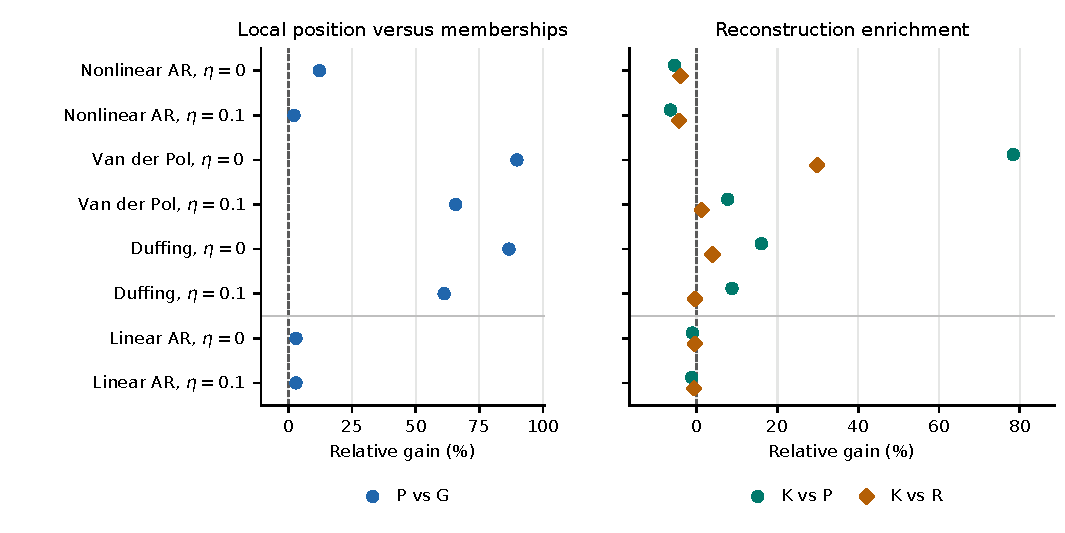
\includegraphics[width=\linewidth]{generated/soft_state_ablation/condition_gains.pdf}
\caption{Descriptive shared-cap gains computed from condition mean
losses. Positive values favor the first arm; dashed lines mark zero
gain. The last two rows are the linear controls, separated by a
horizontal rule. The horizontal scales differ between panels.
No confidence intervals or extra condition-specific superiority tests
are implied by these points.}
\label{supp:sa-condition-gains}
\end{figure}

\begin{table}[htbp]
\centering\small
\caption{Complete descriptive horizon-specific D SMSE means for the
nonlinear (NL) and linear (L) panels. Each horizon is normalized by
its corresponding A target variance before aggregation. The panel
means use equal law/noise weighting within each of
\SARepetitions\ repetitions. These are separately fitted direct
readouts, not successive steps of an autonomous rollout.}
\label{supp:sa-horizons}
% Generated by build_soft_state_assets.py; do not edit.
% Descriptive horizon-specific D SMSE; NL=nonlinear, L=linear. Per-horizon A target variances normalize loss.
\begin{tabular}{@{}llrrrrrr@{}}
\toprule
Cap rule & Arm & NL $h=1$ & NL $h=4$ & NL $h=12$ & L $h=1$ & L $h=4$ & L $h=12$ \\
\midrule
Shared & G & 0.0300446 & 0.0609004 & 0.205666 & 0.811376 & 0.999827 & 1.00592 \\
Shared & P & 0.0122551 & 0.0192541 & 0.059843 & 0.708544 & 1.00821 & 1.01601 \\
Shared & K & 0.0126386 & 0.0192272 & 0.0499322 & 0.718495 & 1.01811 & 1.02653 \\
Shared & R & 0.0120422 & 0.0186757 & 0.0511041 & 0.710428 & 1.01537 & 1.0218 \\
\addlinespace
Independent & G & 0.0300446 & 0.0609004 & 0.205666 & 0.811376 & 0.999827 & 1.00592 \\
Independent & P & 0.0122551 & 0.0192541 & 0.059843 & 0.708544 & 1.00821 & 1.01601 \\
Independent & K & 0.0123713 & 0.0190399 & 0.0488525 & 0.701798 & 1.01751 & 1.0255 \\
Independent & R & 0.0119662 & 0.018509 & 0.0497769 & 0.706971 & 1.01587 & 1.02483 \\
\bottomrule
\end{tabular}

\end{table}

\FloatBarrier
\subsection{Selected dimensions, numerical records, and computation}

The shared P-selected caps $1,2,4,8,12$ occurred in
$31,104,75,32,14$ of the \SATasks\ task suites, respectively.
Tables~\ref{supp:sa-selection} and \ref{supp:sa-selection-panels}
give both cap rules and the separate panel counts. G selected cap
one in every independent-cap task and its aggregate losses did not
change. P's shared and independent selections coincide by construction.
K and R often chose different caps under their own validation
objectives, so their independent-cap comparison no longer holds the
selected bank fixed.

At the shared bank, G used fourteen coordinates; P used $28$--$182$;
and K/R each used $196$--$350$, excluding the intercept. Centered
A feature ranks ranged from $9$--$11$ for G, $23$--$166$ for P,
$186$--$334$ for K, and $180$--$334$ for R. These widths do not
establish a compressed representation of the twelve-dimensional
history. Matching K/R widths does not match their function classes
or effective rank. Five of the $17{,}920$ local-model/cap records
used the native rank-zero wrapper: the same one-reference local
model in one task at each of the five caps. No positive-rank model
required a projected-range reduction. The zero-rank case was retained,
not omitted from evaluation.

Table~\ref{supp:sa-resources} reports measured computation for the
complete search, including rejected candidates and shared bank work.
The summed fit wall time was $931.88$ seconds and the summed D
prediction wall time was $671.84$ seconds. These are sums over worker
tasks, not elapsed time of the three-worker stage. The largest
recorded worker peak RSS was \SAPeakWorkerRSSMiB\ MiB, not an estimate
of simultaneous aggregate memory. Portable NPZ states occupied
\SAStateNPZMiB\ MiB in total; these retain all candidate states
and are not the size of a minimal deployed model. C diagnostic work
is included in the fit totals. Production analysis, independent
auditing, reporting, and archive compression are outside these costs.

The retained analysis records all $76{,}800$ cap/arm/penalty/horizon
B scores as valid. Full numerical solver events, native dimensions,
finite-value safeguards, C predictions, and both selected D views
remain available in the numerical record. The independent audit
passed \SAAuditChecks\ checks across all \SATasks\ tasks. It
independently refitted $25{,}600$ B penalty-path arrays and replayed
$2{,}048$ selected C and $2{,}048$ selected D forecast arrays.
Maximum absolute prediction differences were $1.20\times10^{-11}$
for B, $2.43\times10^{-12}$ for C, and $5.59\times10^{-12}$ for D,
within the frozen replay tolerances $2\times10^{-7}$ relative and
$2\times10^{-9}$ absolute. Source, seal, and stored prefix hashes
were checked exactly; independent numerical replay used the stated
tolerances. The audit also verified references, native ranks, gate
normalization, block transformations, selected penalties, and the
complete primary statistics. There were \SASolverRecoveries\ recorded
SVD-solver recoveries. Its receipt is bound by SHA256 to the released
analysis summary. This is computational verification of the retained
cohort, with the source-order and generator-scope limitations above.

\begin{table}[t]
\centering\small
\caption{B-selected cap frequencies across all \SATasks\ task suites
and selected feature-width/rank ranges. Cap columns count tasks;
the independent inferential sample is still \SARepetitions\
repetitions. Width excludes the intercept, and rank is the centered
A feature-matrix rank. Repeated shared rows reflect one P-selected
bank. Cap twenty is an alias of twelve, not an additional candidate.}
\label{supp:sa-selection}
% Generated by build_soft_state_assets.py; do not edit.
% B-selected cap counts across all 256 task conditions (not independent inferential units); width excludes intercept; centered feature rank on A.
\begin{tabular}{@{}llrrrrrcc@{}}
\toprule
Cap rule & Arm & 1 & 2 & 4 & 8 & 12 & Width range & Rank range \\
\midrule
Shared & G & 31 & 104 & 75 & 32 & 14 & 14 & 9--11 \\
Shared & P & 31 & 104 & 75 & 32 & 14 & 28--182 & 23--166 \\
Shared & K & 31 & 104 & 75 & 32 & 14 & 196--350 & 186--334 \\
Shared & R & 31 & 104 & 75 & 32 & 14 & 196--350 & 180--334 \\
\addlinespace
Independent & G & 256 & 0 & 0 & 0 & 0 & 14 & 9--11 \\
Independent & P & 31 & 104 & 75 & 32 & 14 & 28--182 & 23--166 \\
Independent & K & 67 & 57 & 73 & 42 & 17 & 196--350 & 181--334 \\
Independent & R & 59 & 75 & 89 & 16 & 17 & 196--350 & 177--334 \\
\bottomrule
\end{tabular}

\end{table}

\begin{table}[t]
\centering\small
\caption{Descriptive cap counts separated by population and selection
rule. The nonlinear rows contain $192$ law/noise/repetition task
conditions and the linear rows contain $64$; both populations have
\SARepetitions\ independent repetition units.}
\label{supp:sa-selection-panels}
% Generated by build_soft_state_assets.py; do not edit.
% Descriptive cap counts: 192 nonlinear and 64 linear task conditions, each arising from 32 repetitions.
\begin{tabular}{@{}lllrrrrr@{}}
\toprule
Population & Cap rule & Arm & 1 & 2 & 4 & 8 & 12 \\
\midrule
Nonlinear & Shared & G & 25 & 89 & 61 & 14 & 3 \\
Nonlinear & Shared & P & 25 & 89 & 61 & 14 & 3 \\
Nonlinear & Shared & K & 25 & 89 & 61 & 14 & 3 \\
Nonlinear & Shared & R & 25 & 89 & 61 & 14 & 3 \\
Nonlinear & Independent & G & 192 & 0 & 0 & 0 & 0 \\
Nonlinear & Independent & P & 25 & 89 & 61 & 14 & 3 \\
Nonlinear & Independent & K & 66 & 55 & 50 & 18 & 3 \\
Nonlinear & Independent & R & 56 & 64 & 66 & 4 & 2 \\
\addlinespace
Linear & Shared & G & 6 & 15 & 14 & 18 & 11 \\
Linear & Shared & P & 6 & 15 & 14 & 18 & 11 \\
Linear & Shared & K & 6 & 15 & 14 & 18 & 11 \\
Linear & Shared & R & 6 & 15 & 14 & 18 & 11 \\
Linear & Independent & G & 64 & 0 & 0 & 0 & 0 \\
Linear & Independent & P & 6 & 15 & 14 & 18 & 11 \\
Linear & Independent & K & 1 & 2 & 23 & 24 & 14 \\
Linear & Independent & R & 3 & 11 & 23 & 12 & 15 \\
\bottomrule
\end{tabular}

\end{table}

\begin{table}[t]
\centering\small
\caption{Whole-search resource measurements. All four arms, candidate
caps, and penalties share computations. Task sums of wall time are
not parallel elapsed times; peak worker RSS is not aggregate
concurrent memory. State sizes include all candidates and exclude
the separate retained prediction/data archives. These measurements
do not rank isolated arm costs or establish equal-compute comparisons.}
\label{supp:sa-resources}
% Generated by build_soft_state_assets.py; do not edit.
% Complete search/all four arms. Summed worker wall time is not parallel elapsed time; RSS is not concurrent aggregate memory; state sizes retain all candidates.
\begin{tabular}{@{}lrrr@{}}
\toprule
Measured quantity & Task sum & Task median & Task maximum \\
\midrule
Whole fit wall time (s) & 931.88 & 3.63 & 4.75 \\
Whole fit CPU time (s) & 929.02 & 3.62 & 4.65 \\
D prediction wall time (s) & 671.84 & 2.64 & 3.44 \\
D prediction CPU time (s) & 670.60 & 2.64 & 3.43 \\
Peak worker RSS (MiB) & --- & 155.88 & 156.99 \\
All-candidate NPZ states (MiB) & 177.93 & 0.69 & 0.70 \\
All-candidate JSON states (MiB) & 88.24 & 0.34 & 0.34 \\
\bottomrule
\end{tabular}

\end{table}
\FloatBarrier

\FloatBarrier
\section{Joint input-scaling and dimension-selection study}
\label{supp:joint-selection}

\paragraph{Completed evidence.}
The source was published before production preparation. All 256 tasks
and the independent computational audit have completed, and four
of the six primary criteria are established. The full primary
results appear in Table~\ref{supp:joint-primary}; this section retains
the exact design, additional descriptive results, and verification
scope.

This separate follow-up preserves the G/P/K/R direct-readout
architecture and the completed fixed-standardization experiment.
Its protocol, configuration, and analysis are maintained under
\path{extensions/soft_state_joint_selection_20261102}.
The input transformations, local dimensions, and penalties are
selected jointly using B, while all transformations and model
coefficients are fitted on A. C is diagnostic only. No baseline,
residual correction, calibration, or coordinate-propagation model
is introduced.

\paragraph{Exact scaling rules and candidate order.}
The fifteen candidates iterate through standardization, min--max,
and $\tanh$ of standardized histories, in that order, and then caps
$1,2,4,8,12$ within each scaler. All input-transform statistics are
fitted on the designated A matrix before bank subsampling.
Min--max is $2(x_k-a_k)/(b_k-a_k)-1$ with A extrema $a_k,b_k$;
constant A coordinates map to zero for every query. Subsequent
queries are not clipped. Tanh uses A population mean and scale with
the inherited small-scale rule, and there is no immediate
restandardization of its output. Derived feature blocks are then
standardized and bounded exactly as in the current architecture.
This latter operation is distinct from restandardizing the input.

For every candidate and horizon, each arm selects its own affine
ridge penalty from $10^{-4},10^{-3},10^{-2},10^{-1},1$ on B.
Candidate selection averages the resulting B losses equally over
horizons after division by A-target population variances, floored
at $10^{-12}$. First minima resolve ties at both stages. The selected
states are kept without refitting on B. All controls share a bank
within a candidate, but different scalers can change the partition
and reference allocation.

\paragraph{Four retained views.}
Joint shared selection lets P choose one scaler/cap pair for all
arms. Joint independent selection lets every arm choose its own
pair. Standard-only shared and independent selection restrict the
same fitted grid to its five standardization candidates. Each
task therefore supplies sixteen logical forecast arrays from
fifteen candidate banks. Exact prefix identities hold within a
candidate, not between independently selected geometries.
The paired standard-only comparison separates the effects of
expanding the candidate menu from changes in the simulation cohort.

\begin{table}[tbp]
\centering\small
\setlength{\tabcolsep}{4pt}
\begin{tabular}{@{}lllrr@{}}
\toprule
Search & Geometry & Arm & Nonlinear SMSE & Linear SMSE \\
\midrule
Joint & P-shared & G & 0.0937767 & 0.940694 \\
Joint & P-shared & P & 0.0293596 & 0.915564 \\
Joint & P-shared & K & 0.0267588 & 0.927087 \\
Joint & P-shared & R & 0.0265152 & 0.919841 \\
Joint & Own & G & 0.0921642 & 0.937323 \\
Joint & Own & P & 0.0293596 & 0.915564 \\
Joint & Own & K & 0.0262103 & 0.920881 \\
Joint & Own & R & 0.0259918 & 0.920442 \\
Standard only & P-shared & G & 0.0966196 & 0.943965 \\
Standard only & P-shared & P & 0.029789 & 0.914789 \\
Standard only & P-shared & K & 0.0266938 & 0.922462 \\
Standard only & P-shared & R & 0.0266479 & 0.919456 \\
Standard only & Own & G & 0.0966196 & 0.943965 \\
Standard only & Own & P & 0.029789 & 0.914789 \\
Standard only & Own & K & 0.0262294 & 0.918593 \\
Standard only & Own & R & 0.0260926 & 0.918714 \\
\bottomrule
\end{tabular}

\caption{Mean SMSE in all four retained views of the joint-selection
study. The nonlinear population equally weights its three laws and
two noise conditions within each repetition; the linear population
equally weights its two noise conditions. The displayed means
average the 32 independent repetition aggregates. Each view uses
the same fresh data and the same cached candidate fits.}
\label{tab:joint-aggregate}
\end{table}

\paragraph{Data and inference.}
The fixed design contains 32 new repetitions, four inherited laws,
and two noise levels: 256 tasks. History width is 12, horizons are
1, 4, and 12, origin stride is 4, and A/B/C/D contain
64/32/32/128 independent episodes. A/B/C row caps are 512/256/256;
all 1,664 D origins per task are scored. The new master seed is
2026110204. Its 1,696 declared stream identities are checked
against 8,957 predecessor records, including the completed
soft-state experiment, before production generation. Pairing
across scalers, caps, arms, views, and noise levels follows the
same episode and fitting-stream definitions.

The primary family has six contrasts: joint shared P/G, K/P,
and K/R on the nonlinear population, joint shared K/P on the
linear population, and independently joint-selected K versus
standard-only independently selected K on each population.
The nonlinear margins are 3\% superiority and the linear
margins 5\% noninferiority. One-sided paired Student upper bounds
use $t_{1-0.05/6,31}$ for all six tests. The 32 repetition aggregates,
not individual origins or tasks, are the units of inference.
All other comparisons are descriptive. Gains are ratios of
population mean losses, not means of per-repetition ratios.

\begin{table}[tbp]
\centering\small
\setlength{\tabcolsep}{4pt}
\begin{tabular}{@{}lllrrc@{}}
\toprule
Panel & Contrast & Criterion & Gain (\%) & $U$ & Met \\
\midrule
Nonlinear & $P/G$ & 3\% superiority & 68.69 & -0.0587852 & Yes \\
Nonlinear & $K/P$ & 3\% superiority & 8.86 & -0.00144862 & Yes \\
Nonlinear & $K/R$ & 3\% superiority & -0.9186 & 0.00119423 & No \\
Linear & $K/P$ & 5\% noninferiority & -1.26 & -0.0305374 & Yes \\
Nonlinear & $K_{\mathrm{joint}}/K_{\mathrm{standard}}$ & 3\% superiority & 0.0727 & 0.000901116 & No \\
Linear & $K_{\mathrm{joint}}/K_{\mathrm{standard}}$ & 5\% noninferiority & -0.2491 & -0.0417521 & Yes \\
\bottomrule
\end{tabular}

\caption{Complete six-comparison primary family. The first four
comparisons use P's selected common bank. The last two compare
independently selected K procedures on the identical cohort.
Gain is positive when candidate mean loss is lower; $U$ is the
simultaneous upper bound for the margin-adjusted paired difference.
The criterion is established only when $U<0$.}
\label{supp:joint-primary}
\end{table}

\paragraph{Primary interpretation and descriptive variation.}
The shared-bank P/G and K/P nonlinear comparisons establish their
3\% margins, whereas K/R does not. Both linear noninferiority
criteria are established. The independently selected K comparison
has a nonlinear point gain of \JSGainJointKNonlinear\% against
standard-only K and does not establish its 3\% margin. In particular,
the results do not establish the conjunction of the two direct
tuning criteria. The larger menu weakly improves each arm's selected
B score in the independent view and P's score in the shared view
by construction. That inclusion argument supplies no corresponding
ordering for G, K, or R on P's bank, or for any terminal loss.

Table~\ref{tab:joint-law} reports the law-level point differences
without simultaneous inference. Joint K improves its standard-only
reference on the oscillators and worsens it on both autoregressive
laws. On nonlinear repetition aggregates it wins 15 pairs and loses
17; on the linear aggregates it wins none, ties 18, and loses 14.
These counts describe paired outcomes and are not additional
primary hypothesis tests. Likewise, the independently selected
K/R comparisons describe complete procedures and cannot replace
the failed shared-bank K/R criterion.

\begin{table}[tbp]
\centering\small
\setlength{\tabcolsep}{4pt}
\begin{tabular}{@{}lrrrrr@{}}
\toprule
Law & $K_{\mathrm{standard}}$ & $K_{\mathrm{joint}}$ & $R_{\mathrm{joint}}$ & Joint/standard (\%) & K/R joint (\%) \\
\midrule
Linear AR & 0.918593 & 0.920881 & 0.920442 & -0.2491 & -0.0477 \\
Nonlinear AR & 0.0277254 & 0.0278608 & 0.0265517 & -0.4884 & -4.93 \\
Van der Pol & 0.0244764 & 0.0244209 & 0.0249479 & 0.2269 & 2.11 \\
Duffing & 0.0264863 & 0.0263492 & 0.0264756 & 0.5176 & 0.4773 \\
\bottomrule
\end{tabular}

\caption{Descriptive law-level comparisons of independently selected
procedures. Standard K selects its cap among the five standardized
candidates; joint K and joint R select among all fifteen candidates.
Gains use ratios of mean losses, with positive values favoring K
in the indicated comparison. No law-level margin is established
by this table.}
\label{tab:joint-law}
\end{table}

\paragraph{Selected scalers and native caps.}
Table~\ref{tab:joint-selection-frequency} summarizes the independent
P, K, and R choices. For nonlinear K, standardization is selected
in 91 of 192 tasks, min--max in 64, and tanh in 37. The corresponding
linear counts are 48, 9, and 7 of 64. Selection of a nonstandard
transform records a B preference, not proof of a terminal advantage
for that transform. A cap limits native local dimensions; it is
not the actual rank of every local model. Medians across tasks
can also fall between grid entries: standard-only K's Duffing
median cap is 3 because the middle observations are 2 and 4.
No cap of 3 was fitted.

\begin{table}[tbp]
\centering\small
\setlength{\tabcolsep}{4pt}
\begin{tabular}{@{}llrrrr@{}}
\toprule
Panel & Arm & Standard & Min--max & Tanh & Median cap \\
\midrule
Nonlinear & P & 78 (40.6\%) & 71 (37.0\%) & 43 (22.4\%) & 2 \\
Nonlinear & K & 91 (47.4\%) & 64 (33.3\%) & 37 (19.3\%) & 2 \\
Nonlinear & R & 82 (42.7\%) & 69 (35.9\%) & 41 (21.4\%) & 2 \\
Linear & P & 31 (48.4\%) & 28 (43.8\%) & 5 (7.8\%) & 8 \\
Linear & K & 48 (75.0\%) & 9 (14.1\%) & 7 (10.9\%) & 8 \\
Linear & R & 32 (50.0\%) & 28 (43.8\%) & 4 (6.2\%) & 8 \\
\bottomrule
\end{tabular}

\caption{Independent joint selections by population and arm. Scaler
counts sum to 192 nonlinear or 64 linear tasks per arm. Reported
cap summaries concern selected upper bounds, not a common realized
local rank. Frequencies are descriptive and use B alone.}
\label{tab:joint-selection-frequency}
\end{table}

\paragraph{Verification scope.}
Manufactured-only preflight checks compare standard-only behavior
with the published model, independently reconstruct every scaler's
A statistics and query transforms, verify shared block prefixes,
native cap aliases, ridge and geometry selection, and portable-state
roundtrips. A miniature staged fixture exercises the source freeze,
publication requirement, global fitted-state and prediction seals,
target release, and independent audit. These fixtures supply no
scientific outcome evidence.

The completed production audit passed \JSAuditChecks\ checks on
all \JSTasks\ tasks. It independently reconstructed all
76,800 B penalty-path forecast arrays, 4,096 selected C arrays,
and 4,096 selected D arrays. Maximum absolute differences were
$1.13\times10^{-10}$, $2.42\times10^{-12}$, and
$6.28\times10^{-12}$ respectively. It verified the A-fitted
input statistics, all fifteen candidates, native dimensions,
shared-prefix identities, selections, standard-only references,
stage and data rosters, and independently recomputed all six
primary and 64 descriptive paired comparisons. There were
\JSSolverRecoveries\ numerical solver recoveries.
The declared general replay tolerances remained
\texttt{rtol=2e-7}, \texttt{atol=2e-9}, with tighter checks where
specified. The audit uses the saved fitted geometry and physical
episodes; it does not independently refit partition k-means or
reintegrate the physical laws. Computational replay is not
independent scientific replication.

\paragraph{Measured resource scope.}
The core candidate-fitting records sum to \JSFitCpuMinutes\ CPU minutes and
\JSFitWallSumMinutes\ worker wall minutes, with a median of
\JSFitMedianSeconds\ wall seconds per task. The prediction-task
records sum to \JSQueryWallSumMinutes\ worker wall minutes.
These are sums over tasks, not elapsed end-to-end runtime.
They cover the declared candidate search and shared computations;
they do not isolate the cost of K or establish computational parity
with R. Portable fitted states, all candidate B paths, selected C
and D forecasts, raw episodes, and released targets are retained
in the indexed numerical records. The main paper and this
supplement compile from the included display assets without model
fitting or these large archives.
\FloatBarrier

\FloatBarrier
\section{Predictive usefulness and computational cost}
\label{sec:utility-question}
Let $X\in\R^d$ be an observed history, $Y\in\R^{d_y}$ its future
response, and $\Gamma_{\mathcal D}$ a representation fitted on development
data $\mathcal D$. Expectations below are conditional on the fitted
state. The map $\Gamma_{\mathcal D}$ may contain soft memberships,
signed local observables, or a study-specific geometric encoding; no
simplex constraint is imposed on this general notation. The response
$Y$ is specified by the prediction task, so its loss measures usefulness
for that response rather than ease of predicting the encoding itself.
Each experiment specifies its own evaluation distribution and
loss aggregation. A deterministic representation can discard predictive
information; appending it to $X$ preserves the raw history and hence its
Bayes risk (Proposition~\ref{prop:nf-raw-preservation}). This does not
ensure equal performance of finite, regularized fitted decoders.

\paragraph{Residual information relative to a baseline.}
Fix $f_0:\R^d\to\R^{d_y}$, put $e=Y-f_0(X)$ and
$Z=\Gamma_{\mathcal D}(X)$, and assume $\E\|e\|_2^2<\infty$.
Write $R(f)=\E\|Y-f(X)\|_2^2$ and let
$L^2(P_Z;\R^{d_y})$ contain the measurable corrections with finite
second moment under the distribution $P_Z$ of $Z$. Conditional
expectation gives the best correction $q^*(Z)=\E[e\mid Z]$ and
\begin{equation}\label{eq:utility-oracle}
 R(f_0)-\inf_{q\in L^2(P_Z;\R^{d_y})}
 R(f_0+q\circ\Gamma_{\mathcal D})
 =\E\|\E[e\mid Z]\|_2^2.
\end{equation}
The circle denotes composition. Appendix~\ref{app:utility-projection}
proves the identity. Improvement is possible in this unrestricted
correction class precisely when the residual conditional mean is
nonzero with positive probability. The identity does not determine the
performance of a correction estimated in a finite class.

\paragraph{Fitted procedures and computation.}
For fitted forecasts $\widehat f_0$ and $\widehat f_s$, evaluation unit
$\mathcal E$, and specified squared loss $\ell$, define
\begin{equation}\label{eq:utility-delta}
 \Delta_s=\E[\ell(\widehat f_0;\mathcal E)
             -\ell(\widehat f_s;\mathcal E)\mid\mathcal D].
\end{equation}
Positive $\Delta_s$ favors the richer procedure. A comparison may require
a minimum gain $\delta>0$ and cost budget $B>0$, with measured complete
procedure cost $C_s\leq B$. Feature construction, fitting, and selection
are charged even when the selected prediction equals the baseline.
Evaluation outcomes cannot enter fitting or selection. Independently
sampled repetitions, overlapping windows, and selected source families
supply different units of evidence. Missing predictions without a
prespecified fallback make the affected full-roster aggregate undefined;
restriction to successful fits changes the evaluated population. No
experiment here estimates unrestricted natural-data Bayes risk or
certifies the minimum complexity necessary to achieve a target accuracy.

\paragraph{A correction that retains the fitted baseline.}
For geometric family $g$, fitted correction $\widehat q_g$, and scalar
mixing weight $\gamma$, define
\begin{equation}\label{eq:utility-additive}
 \widehat f_{g,\gamma}(x)
 =\widehat f_0(x)+\gamma\widehat q_g(x),\qquad 0\leq\gamma\leq1.
\end{equation}
Zero correction recovers the same fitted baseline. Residual fitting is
established \citep{Buhlmann2003L2}; these studies compare the geometric
features supplied to the correction. With square-integrable residual
and correction, expansion of squared loss yields
\begin{equation}\label{eq:utility-alignment}
 R(\widehat f_{g,\gamma})-R(\widehat f_0)
 =\gamma^2\E\|\widehat q_g(X)\|_2^2
 -2\gamma\E\langle Y-\widehat f_0(X),\widehat q_g(X)\rangle.
\end{equation}
Here $\langle\cdot,\cdot\rangle$ is the Euclidean inner product.
For a correction nonzero with positive probability, positive expected
alignment is necessary and sufficient for improvement at some
sufficiently small positive $\gamma$. A finite candidate grid may miss
that interval, and validation can select a worse forecast. Baseline
availability is therefore a candidate-class property, not a performance
guarantee; Appendix~\ref{app:utility-alignment} gives the derivation.

\section{Geometry, predictive encoding, and decoder access}\label{c:sec:method}

\paragraph{Matched reconstruction rules.}
Let $z\in\R^d$ be a column vector obtained by standardizing an input with
training-set means and standard deviations. The controlled study fits three
independent $k$-means partitions, with $2$, $4$, and $8$ local models,
respectively. Index the resulting $14$ models by $c$. Model $c$ contains
$n_c\leq24$ reference observations, stored as the rows of
$V_c\in\R^{n_c\times d}$. Let $\mu_c\in\R^d$ be their mean and let
$P_c\in\R^{d\times p_c}$ contain orthonormal principal directions, where
$p_c\leq\min(2,d-1,n_c-1)$ is the effective local rank under the
explicit constrained policy of these supporting studies. It is not the
native KAHM default-cap rule. Input scaling,
partitions, references, principal directions, and the score construction
are shared by the two reconstruction rules:
\begin{equation}\label{c:eq:affine}
 r_c^{\A}(z)=\mu_c+P_cP_c^\top(z-\mu_c),\qquad
 r_c^{\K}(z)=
 \frac{V_c^\top B_c k_c(z)}{\boldsymbol 1_{n_c}^\top B_c k_c(z)}.
\end{equation}
Here $k_c(z)\in\R^{n_c}$ contains the Gaussian similarities between the
query and the reference observations in the local projected covariance
metric; $B_c\in\R^{n_c\times n_c}$ is the symmetric regularized inverse of
the reference kernel matrix; and $\boldsymbol 1_{n_c}$ is the vector of
$n_c$ ones. Appendix~\ref{c:app:methods} specifies the kernel, regularizer,
and treatment of degenerate banks. The normalized KAHM weights can be
negative. In the controlled implementation, reference values are stored in
32-bit floating-point precision, and an exactly zero reconstruction
denominator is replaced by one. A separate numerical sensitivity analysis
examines Gaussian underflow. Sharing the bank makes this a comparison of
reconstruction operators within one specified procedure.

\paragraph{The features supplied to the predictor.}
For either reconstruction $r_c$, define a radial discrepancy $q_c$ and an
angular discrepancy $b_c$ by
\begin{align}
 q_c(z)&=1-\exp\{-\|z-r_c(z)\|_2\},\qquad
 b_c(z)=\pi^{-1}\arccos\!\left(\clip\!\left(
 \frac{\langle z,r_c(z)\rangle}{\|z\|_2\|r_c(z)\|_2},-1,1\right)\right),
 \nonumber\\[-2pt]
 T_c(z)&=\sqrt{\{q_c(z)^2+b_c(z)^2\}/2},\qquad
 w_c(z)=(1-T_c(z)+\tau)^\omega,\qquad
 \phi_c(z)=\frac{w_c(z)}{Z_{b(c)}(z)},\label{c:eq:phi}
\end{align}
where $\clip(u,a,b)=\min\{b,\max\{a,u\}\}$, $\tau=10^{-6}$, and
$\omega=16$. If the denominator in the cosine is zero, its value before
clipping is defined to be zero. The index $b(c)\in\{1,2,3\}$ identifies
the partition containing model $c$, and
$Z_b(z)=\sum_{j:b(j)=b}w_j(z)$ is that partition's normalizing constant.
Thus the affinities sum to one within each partition. Let
$\phi(z)\in\R^{14}$ and $\mathbf T(z)\in\R^{14}$ be the concatenated
affinity and score vectors, respectively. The feature comparisons provide
the decoder with affinities, full scores, one $\log Z_b$ per partition,
raw inputs, or gated local coordinates. The last construction is
\begin{equation}\label{c:eq:local}
 \Gamma_{\rm local}(z)=
 \operatorname{col}\!\left(
 \phi(z),\{\phi_c(z)P_c^\top(z-\mu_c)\}_{c=1}^{14}\right),
\end{equation}
where $\operatorname{col}$ concatenates its column-vector arguments. This
is a local-tangent feature construction \citep{Yu2010LTC}; the study
examines how the geometric gates affect prediction.

Two information properties follow directly from these definitions. First,
the score normalization has the inverse
\begin{equation}\label{c:eq:inverse}
 T_c(z)=1+\tau-
 \exp\{(\log\phi_c(z)+\log Z_{b(c)}(z))/\omega\}.
\end{equation}
Consequently, $\mathbf T$ and the pair consisting of $\phi$ and all three
log normalizers retain the same information in exact arithmetic. Their
finite fitted decoders can nevertheless have different risks because the
inverse is nonlinear. Second, suppose all gates are positive and the
matrix formed by stacking $P_c^\top$ has full column rank $d$. Dividing
the local-coordinate blocks by their gates recovers $P_c^\top(z-\mu_c)$.
Adding $P_c^\top\mu_c$ then yields a full-rank linear system for $z$.
Proposition~\ref{c:prop:local-injectivity} makes this argument precise.
The $144$ inspected controlled forecasting banks have full numerical rank
and positive gates on their evaluated inputs. These checks do not establish
uniformly positive gates or a stable inverse on the entire input domain
(Appendix~\ref{c:app:review-diagnostics}). Conversely, a rank-deficient
stack does not by itself establish information loss, because the gates
may encode additional distinctions between inputs.

\paragraph{A controlled target intervention.}\label{c:sec:controlled}
Let $S$ take the values $-1$ and $+1$ with equal probability, let
$T\sim\mathrm{Unif}[-1,1]$, and let
$\epsilon\sim\mathrm{Unif}[-0.1,0.1]$. Assume these three variables are
independent. For curvature $c\in\{0,1\}$ and target-mixture weight
$\lambda\in\{0,\tfrac12,1\}$, define
\begin{equation}\label{c:eq:branch}
 X=\begin{pmatrix}T\\c\cos(\pi T)+0.5S\end{pmatrix},\qquad
 Y_\lambda=\sqrt{1-\lambda}\,S+\sqrt{3\lambda}\,T+\epsilon.
\end{equation}
Here $S$ identifies the branch and $T$ gives position along it. Within each
repetition and curvature, changing $\lambda$ leaves the input observations,
noise, and fitted bank unchanged. The predictable signal has variance one,
and the Bayes mean squared error is $\operatorname{Var}(\epsilon)=1/300$.
As $\lambda$ increases, the target changes from branch identity to signed
position. Its accessibility to a particular decoder can change even though
the signal and noise variances remain fixed.

Define the reflection $Q(x_1,x_2)=(-x_1,x_2)$. A representation satisfying
$\Gamma(QX)=\Gamma(X)$ cannot retain the sign of the position component
$\sqrt{3\lambda}T$. Its Bayes mean squared error is therefore at least
$1/300+\lambda$. There is also a quantitative statement for an approximately
invariant representation. Let $d_U$ be a pseudometric on its feature space,
let $g$ be a decoder satisfying
$|g(u)-g(v)|\leq\kappa d_U(u,v)$ for all feature values $u,v$, and define
\begin{equation}\label{c:eq:symmetrybound}
 R(g\circ\Gamma)-R_X^{\rm Bayes}
 \geq\left(\sqrt\lambda-\kappa\delta_\Gamma/2\right)_+^2,
 \qquad
 \delta_\Gamma^2=\E[d_U(\Gamma(X),\Gamma(QX))^2].
\end{equation}
In this expression $R(f)=\E[(Y_\lambda-f(X))^2]$,
$R_X^{\rm Bayes}=1/300$, and $(a)_+=\max\{a,0\}$; the claim assumes the
quantities are square-integrable. A pseudometric satisfies the usual
metric inequalities but may assign distance zero to distinct points.
Appendix~\ref{c:app:theory} proves both the exact and approximate statements.
The measured reflection differences are descriptive estimates: they do not
supply a population upper bound for $\delta_\Gamma$, and the fitted
experimental decoders have no imposed common Lipschitz budget.

The complete branch results and reconstruction and scoring diagnostics
are reported in Appendix~\ref{c:app:tables}. Affine local coordinates
recover accurate position prediction in the straight-branch example;
the information advantage there is not exclusive to nonlinear KAHM
reconstruction.

\section{Conditional gains in controlled forecasting}\label{c:sec:capacity}

The controlled forecasting laws are nonlinear autoregression (AR),
Van der Pol, and Duffing. Each repetition independently generates 128
training, 128 validation, and 512 test episodes of length 72. Histories
have length 12 and predict offsets 1, 4, and 12 at 13 origins per episode.
Entire episodes stay within a split; MSE averages origins and horizons
within episodes and then episodes. Appendix~\ref{c:app:methods} specifies
the numerical generators and fitting rules.

The first study has 24 full data-and-fit repetitions in each of nine
primary settings: six target functions on the branch construction and three forecasting laws. Adding
local coordinates to KAHM affinities improves ridge prediction beyond the
fixed practical margin in \LocalPracticalBenefitCount{} settings. On Van
der Pol, mean MSE falls from $\VDPPhiRidgeMSE$ to
$\VDPKAHMLocalRidgeMSE$, although affine local coordinates perform better
with the same ridge head. The first study uses 95\% Bonferroni-adjusted paired Student intervals
for a family of 29 contrasts. This supports retaining local position,
while leaving the complete representation--decoder choice unresolved.

A follow-up specifies its candidate models, practical margins, and
analysis before generating 24 additional independent repetitions per
forecasting law. It compares raw histories, affine local features, KAHM local features,
and full KAHM scores with 64 or 256 Gaussian Nystr\"om landmarks. The
head appends linear coordinates to the finite nonlinear basis, standardizes
basis columns, and uses an ordinary Euclidean ridge penalty. Validation
selects among three bandwidth multipliers and seven penalties; the fitted
model uses training observations only. Equal landmark counts do not imply
equal realized ranks, function classes, or computational costs.

Table~\ref{c:tab:all-capacity} reports the complete comparison family. KAHM local features outperform raw and affine local features
on Van der Pol at both widths in every repetition. At 256 landmarks,
mean MSEs are $\VDPKAHMWideMSE$, $\VDPRawWideMSE$, and
$\VDPAffineWideMSE$, respectively: descriptive reductions of
\VDPRawWideRelativeGain\% and \VDPAffineWideRelativeGain\% relative to the
controls. The two simultaneous lower endpoints, $0.00075496$ and
$0.00018100$, exceed the prespecified practical margin $0.00014891$; both
64-landmark comparisons also clear it. Raw inputs win on AR at both
widths, and both controls win on Duffing. KAHM--affine differences on AR
remain unresolved. The separate 29- and 12-contrast families do not imply
a joint 95\% coverage statement. Their inferential units are complete
repetitions, not windows or horizons (Appendix~\ref{c:app:statistics}).

\paragraph{Numerical sensitivity and an adverse natural-data check.}
\label{c:sec:numerical}
The original Gaussian query evaluation can produce an all-zero row before
signed normalization. Writing $\ell_j$ for a query log-kernel entry, replacing
$\exp\ell_j$ by
$\exp(\ell_j-\max_i\ell_i)$ preserves exact normalized weights whenever
the denominator is nonzero (Proposition~\ref{c:prop:inner-scaling}). In a
post-hoc check reusing the 24 Van der Pol follow-up samples and banks, with
affected heads refitted and validation-tuned, exactly zero normalizers fall
from \NumericalOriginalZeroCount{} among \NumericalQueryClusterCount{}
query--local-model evaluations to zero. KAHM-local mean MSE changes by
less than $4\times10^{-13}$ at either width, whereas full-score losses
improve by roughly $0.37$--$0.39\%$. Row scaling addresses this underflow
pathway; it does not prevent signed cancellation or establish stability on independently generated data.

On a fixed grouped split of Airfoil Self-Noise \citep{Brooks1989Airfoil},
raw RBF obtains mean group-weighted MSE $\AirfoilRawRBFMSE$ dB$^2$,
compared with $\AirfoilKAHMLocalRBFMSE$ for KAHM-local RBF. The validation selector chooses
raw RBF in all 24 fits. These seeds characterize fitting variability on
one static-regression dataset and split, not independent natural
forecasting evidence. Together, the controlled results motivate testing
local features as conditional candidates. The branch symmetry result does not explain the Van der Pol gain,
and these simulations do not establish transfer to new source families;
Section~\ref{sec:natural} examines that question separately.

\section{Natural forecasting: transfer, cost, and predicting benefit}\label{sec:natural}
The study fixes four development families (Electricity, NN5, Tourism,
and FRED-MD) and four confirmation families (Traffic, Hospital, Saugeen
River flow, and US births). Training-prefix eligibility and identifier
hashes select 26 series. Two history--horizon regimes, two capacities,
and two seeds yield 208 runs, including 80 confirmation runs. Every
method uses the same available windows and chronological 60/20/20
splits. All fitted transformations use permitted training observations;
validation selects hyperparameters, and a final fit uses eligible
pretest windows. Appendix~\ref{sec:nf-methods} defines all twelve
procedures; Appendix~\ref{sec:nf-protocol} supplies source versions,
chronology, capacity grids, loss scales, selection rules, and cost scopes.
The four confirmation families remain the units of transfer despite
multiple configurations and overlapping windows within them.

The primary matched comparison is raw finite-RBF prediction against
raw history augmented by KAHM gates and gated principal coordinates.
The augmentation preserves history information, but changes Gaussian
distances, the finite basis, and regularization. All 208 runs complete
with every candidate present, yielding 2,496 task--method losses.
Raw plus KAHM has \NaturalErrorIncrease\% higher source-balanced loss
than raw RBF at \NaturalCostRatio{} times its measured warm-library
pipeline cost; raw ridge is more accurate than both
(Table~\ref{tab:method-summary}). KAHM raises loss against raw RBF by
0.50\% on Traffic, 12.27\% on Hospital, and 3.53\% on US births,
and lowers it by 1.53\% on Saugeen. Omitting any one confirmation
family leaves the aggregate unfavorable. These are descriptive selected-source
comparisons, without population-wide confidence intervals.

The structural controls and development results further limit
attribution. Raw plus KAHM improves aggregate loss over raw plus affine
and raw plus locality by only 0.46\% and 0.50\%, respectively; each
comparison changes sign across source means. FRED-MD contributes
96.62\% of the development gain over raw RBF, while raw plus affine
has lower mean loss and cost than KAHM in every development family.
Table~\ref{tab:cleanup-costs} separates substantial selection cleanup
from search and refitting. The reported 2.30-fold ratio describes the
supplied warm workflow, not cold-start deployment or intrinsic complexity.

Four ridge diagnostics predict log relative benefit from metadata,
geometry, a reduced-capacity validation probe, or their combinations.
They are trained on development outcomes with whole-source exclusions
and frozen before confirmation (Section~\ref{sec:nf-diagnostic}). Adding
geometry to metadata plus the paid probe changes none of the 80
confirmation decisions. Both variants attain scaled MSE
\NaturalProbeLoss{} at about \NaturalProbeCost{} seconds per task;
log-benefit RMSE increases from 0.184549 to 0.184680. Their aggregate
gain over always raw is only \NaturalProbeGainPercent\%, at
\NaturalProbeCostRatio{} times its pipeline cost. Metadata plus geometry
also makes the same decisions as metadata alone. Complete methods,
policies, source outcomes, and diagnostic predictions appear in
Appendix~\ref{app:full-results}. These data do not validate the tested
geometric adoption rule; they do not rule out a different diagnostic.

\section{Post-hoc sensitivity to geometry scaling}\label{sec:scaling}
A specified sensitivity analysis replaces training z-score geometry
scaling by training min--max scaling to $[-1,1]$, without clipping
future values. Raw-history components and comparators remain
standardized. Targets, splits, seeds, head grids, capacities, and query
conventions are fixed. The protocol precedes these fits but follows
inspection of the original outcomes. These paired comparisons reuse
sources and draws and supply no fresh confirmation.

All 208 natural configurations are rerun for the three raw-augmented
geometries under both scalers. On the four formerly reserved families,
KAHM loss changes from \ScalingNaturalKahmStandardLoss{} to
\ScalingNaturalKahmMinmaxLoss{}, an increase of
\ScalingNaturalKahmChangePercent\%. Min--max KAHM remains
\ScalingNaturalKahmVsRawPercent\% above raw RBF and
\ScalingNaturalKahmVsRidgePercent\% above ridge. Its measured warm
method time is \ScalingNaturalKahmMinmaxTime{} seconds, compared with
\ScalingNaturalKahmStandardTime{} for standardized KAHM and
\ScalingNaturalRawTime{} for the remeasured raw RBF. The timings include
a retained Saugeen search/cleanup outlier and do not identify an intrinsic
cost of scaling.

All 24 original controlled draws per law and both landmark counts are
also reused. The principal ordering persists: raw RBF is better on
autoregression and Duffing, while KAHM local features are better than
raw and both local controls on Van der Pol. Individual changes can be
substantial: 256-landmark Duffing KAHM MSE falls by 7.35\%, yet remains
above the raw, affine, and locality controls. Appendix~\ref{app:scaling}
retains the complete paired cells, source heterogeneity, and resource
accounting. The original benefit diagnostic is not refitted or reevaluated
under min--max geometry.

\section{Preserving raw forecasts while testing geometric utility}
\label{sec:utility-extension}

An additive experiment separates the contribution of KAHM features
from changes to the raw predictor. It tests whether a local geometric
correction improves a fixed raw forecast, how this improvement depends
on training size and raw-decoder capacity, and whether a validation
rule identifies useful corrections on four additional archive collections.
The protocol, candidate grid, source roster, and implementation were
archived before full evaluation. This was a prospective execution
checkpoint informed by earlier findings, without external preregistration.

\subsection{Forecasts, controls, and selection}
\label{sec:utility-models}

The raw baseline is a finite Gaussian Nystr\"om predictor with
appended linear history coordinates, column standardization, and a ridge
head. Its requested $M$ landmarks and regularization are fitted using the raw history
only. For each $g\in\{\mathrm{KAHM},\mathrm{affine},\mathrm{locality}\}$,
we fit a separate ridge head on the local-coordinate features of
Equation~\eqref{c:eq:local}, using the raw model's training residuals as
targets. The additive forecast is Equation~\eqref{eq:utility-additive}.
The correction has its own standardization and ridge penalty; it does not
change raw distances, landmarks, coefficients, or regularization, and it
introduces no additional Nystr\"om basis. Residuals are in-sample training
residuals, not cross-fitted residuals. This choice is part of the evaluated
procedure and can limit the structure left for the correction to learn.

All geometries use the same partitions, principal-direction configuration,
reference-selection rules, and fitting seeds. The geometry bank uses
three blocks of 2, 4, and 8 local models, requested rank two, at most 24
references per local model, and at most 512 fitting histories. KAHM uses
the stable Gaussian query arithmetic described in
Section~\ref{c:sec:numerical}; affine and locality controls do not fit KAHM
kernels. The concatenated raw-plus-KAHM architecture from the original
natural study is also fitted under this extension's limits. It preserves
raw information but changes the finite kernel geometry, so it is a
different complete procedure, not a restricted version of the additive
model. Raw ridge, persistence/seasonal-naive prediction, and a fixed
histogram-gradient-boosting control complete the comparison.

Validation first chooses the raw RBF penalty from
$\{0.01,1,100\}$. Holding this raw forecast fixed, each correction searches
the same three penalties and weights $\gamma\in\{0,0.25,0.5,1\}$.
There are ten distinct correction candidates: one zero correction and
nine positive-weight choices. Ties favor smaller $\gamma$, followed by
the fixed penalty order. These extra validation opportunities are part
of the additive procedure; equal landmark counts do not equalize search
size, effective function classes, or cost. The main KAHM policy uses its
selected correction only if validation MSE is at least 5\% below that of
the selected raw baseline. A second declared policy applies the same
threshold to the validation-best choice across all three geometries.
The 5\% threshold is a research sensitivity, not a test-set guarantee or
an application-derived minimum. Every policy pays for the corrections
it examines, including corrections it declines.

\subsection{Training size, raw-decoder capacity, and archive sources}
\label{sec:utility-design}

The synthetic factorial crosses the three forecasting laws in
Appendix~\ref{c:app:methods},
$N\in\{32,128\}$ independent training episodes, and
$M\in\{16,64\}$ raw RBF landmarks. Twelve fresh repetitions use seeds
9100--9111, for 144 configurations. Within a law and repetition, the 32
training episodes are a prefix of the same 128-episode collection, and
all four $N\times M$ settings share 64 validation and 128 test episodes.
Episodes retain length 72, history 12, offsets 1, 4, and 12, and 13 origins
per episode. All training origins can fit the decoder; the 512-history
limit applies only to the geometry bank. Selected forecasts use
training-only fitting, without adding validation episodes, so $N$ remains
an interpretable factor. This changes the raw predictor's capacity while
holding the correction's declared architecture fixed; it does not vary
every source of model complexity.

Synthetic MSE averages target coordinates and origins within episodes,
then episodes. The primary loss differences compare additive KAHM with
raw RBF and concatenated KAHM in each of the 12 law--$N$--$M$ cells.
All 24 contrasts use a separate family of 95\% Bonferroni paired Student
intervals over 12 complete repetitions. Their coverage relies on a
normal approximation for repetition-level differences; origins and
horizons do not increase the replication count. Affine, locality, and
practical-control means are reported without promoting their descriptive
comparisons into that primary interval family.

The archive-source evaluation uses Weather, Solar Weekly, COVID-19 Deaths,
and Car Parts with missing values from the Monash archive
\citep{Godahewa2021Monash,Godahewa2020Weather,Godahewa2020SolarWeekly,
Godahewa2020CovidDeaths,Godahewa2020CarPartsMissing}. They were absent
from the original eight-source study. Solar Weekly is an aggregation
of simulated NREL solar-production series; it is not an independent
observational solar deployment. Three training-prefix-eligible series
per collection are selected by a fixed hash ordering. Eligibility and
selection cannot use validation/test forecasting performance, and selected
series are not replaced because later evaluation is unfavorable or
unavailable. The roster is listed in Appendix~\ref{app:utility-protocol}.

Each series has chronological 60/20/20 training, validation, and test
segments. Weather and COVID use a 28-step history and all seven next
steps as direct targets; Solar Weekly and Car Parts use a six-step
history and two-step target. Fits use at most 512 available training
windows and evaluations at most 64 origins per segment, sampled evenly.
After validation selection, selected configurations are refitted on
admissible pretest windows under the same cap. Inputs use only past
observations, including already observed test values at later origins;
test targets cannot retune the fitted model. Missing values are not
interpolated. A training-only seasonal-difference MSE, with a declared
first-difference fallback, supplies the fixed scale. The two requested landmark
counts give 24 configurations. Aggregation weights capacities equally
within series, series equally within source, and the four sources equally.
These are descriptive comparisons on four selected collections, not
24 independent domains or a random sample of applications.

The main model-pipeline cost covers raw search, geometry and correction
search, validation forecasts, selected refits, final prediction, and model
serialization. Shared raw work is charged once for an additive procedure
or policy. Data preparation is recorded separately, as are model size and
prediction cost. Imports, downloads, prediction-artifact writes, and
research reporting are outside model timing. Policy costs are unions of
measured required components, not separately timed full-policy executions.
One task and one numerical-library
thread are active during timing. Wall time and available CPU components
are recorded separately. The accuracy--cost comparison therefore
describes this implementation and hardware, without claiming a minimum
necessary representation complexity. Additional fitting and audit details
appear in Appendix~\ref{app:utility-protocol}.

\subsection{Complete outcomes and fit coverage}
\label{sec:utility-synthetic-results}\label{sec:utility-archive-results}
Tables~\ref{tab:utility-synthetic}, \ref{tab:utility-synthetic-controls},
and~\ref{tab:utility-intervals} report every synthetic cell and primary
contrast. Five of twelve comparisons with raw RBF favor additive KAHM,
none favors raw RBF, and seven remain unresolved. Against concatenated
KAHM, six favor the additive construction, four favor concatenation,
and two remain unresolved. Simpler additive geometries have lower mean
error in every Van der Pol and Duffing cell; the raw-baseline contrasts
do not establish an advantage specific to KAHM.

% Generated from the audited forecasting-utility extension; no model fitting.
\begin{table}[!htbp]
\centering\small\setlength{\tabcolsep}{4pt}
\caption{New synthetic factorial: mean test MSE multiplied by $10^3$, over 12 fresh complete repetitions per cell. $N$ counts training episodes; $M$ counts raw RBF landmarks. All correction heads are ridge heads. These are cell means; simultaneous primary intervals appear in Table~\ref{tab:utility-intervals}.}
\label{tab:utility-synthetic}
\begin{tabular}{lrrrrrrr}
\toprule
Law & $N$ & $M$ & Raw RBF & Concat. & +KAHM & +Affine & +Locality \\
\midrule
Nonlinear AR & 32 & 16 & 4.8715 & 4.9851 & 4.7525 & 4.7586 & 4.7584 \\
Nonlinear AR & 32 & 64 & 5.0133 & 5.3388 & 5.0157 & 5.0190 & 5.0173 \\
Nonlinear AR & 128 & 16 & 4.6648 & 4.6592 & 4.5701 & 4.5805 & 4.5753 \\
Nonlinear AR & 128 & 64 & 4.4806 & 4.7006 & 4.4806 & 4.4840 & 4.4832 \\
Van der Pol & 32 & 16 & 22.0913 & 7.0925 & 15.6100 & 15.1578 & 12.8848 \\
Van der Pol & 32 & 64 & 9.2066 & 2.6518 & 8.2892 & 8.3880 & 8.0522 \\
Van der Pol & 128 & 16 & 20.5463 & 7.5690 & 14.4955 & 13.8986 & 11.5027 \\
Van der Pol & 128 & 64 & 8.4031 & 2.4087 & 7.4507 & 7.5359 & 7.0687 \\
Duffing & 32 & 16 & 7.3080 & 8.5619 & 6.6154 & 5.3215 & 5.6464 \\
Duffing & 32 & 64 & 5.3159 & 5.0348 & 5.2959 & 4.7693 & 5.0240 \\
Duffing & 128 & 16 & 6.6937 & 7.6252 & 5.8873 & 4.7225 & 4.8299 \\
Duffing & 128 & 64 & 4.3215 & 4.0529 & 4.2667 & 3.6788 & 3.8379 \\
\bottomrule
\end{tabular}
\end{table}


All 144 synthetic configurations complete. On the archive roster, 22
of 24 configurations complete every procedure. Both capacities of Car
Parts T1324 have 23 training histories but only seven distinct ones;
the declared eight-group bank fails. Concatenated KAHM and all three
additive geometries fail on both configurations, giving eight failed
fits and four unavailable dependent policy outputs. These are shared
bank-fitting failures, not an isolated KAHM-kernel failure. Raw ridge,
raw RBF, naive, and boosting complete all 24 configurations.

% Generated from the audited forecasting-utility extension; no model fitting.
\begin{table}[!htbp]
\centering\small\setlength{\tabcolsep}{4pt}
\caption{New archive-source coverage and losses. Full-roster scaled MSE uses all 24 configurations and is undefined (dash) for procedures with failed fits. Matched loss and wall seconds use only the post-hoc 22-configuration common-support diagnostic (11 series, including two Car Parts series), with equal source weights. Pipeline costs include all required searches, validation, selected refit, prediction, and serialization. Policy costs are unions of measured required components, including rejected corrections; they are not separately timed full policy executions. Conditioning on success does not complete the prespecified full-roster evaluation.}
\label{tab:utility-archive}
\begin{tabular}{lrrrr}
\toprule
Procedure & Outputs & Full-roster MSE & Matched MSE & Matched seconds \\
\midrule
Raw ridge & 24/24 & 1.2848 & 0.8466 & 0.0015 \\
Raw RBF & 24/24 & 9.6633 & 9.1730 & 0.0037 \\
Concatenated KAHM & 22/24 & \textemdash & 1.2111 & 0.0691 \\
Additive KAHM & 22/24 & \textemdash & 9.1443 & 0.0498 \\
Additive affine & 22/24 & \textemdash & 9.3312 & 0.0369 \\
Additive locality & 22/24 & \textemdash & 9.5624 & 0.0379 \\
Persistence / seasonal naive & 24/24 & 1.5720 & 1.2062 & 0.0012 \\
Histogram gradient boosting & 24/24 & 10.7552 & 10.3174 & 0.6380 \\
KAHM 5\% rule & 22/24 & \textemdash & 9.2460 & 0.0467 \\
All-geometry 5\% rule & 22/24 & \textemdash & 9.2624 & 0.0869 \\
\bottomrule
\end{tabular}
\end{table}


The full-roster geometric and policy losses are undefined. The separate
post-hoc matched-success analysis conditions on 22 configurations,
with eleven series and equal source weights. Additive KAHM gains only
\UtilityKAHMGainPercent\% over raw RBF at \UtilityKAHMCostRatio{}
times its measured model-pipeline cost; ridge is more accurate and
cheaper. Neither policy improves aggregate loss on this subset. COVID
is the only source mean improved by additive KAHM, Solar is unchanged,
and Weather and Car Parts worsen; excluding COVID reverses the
aggregate direction. Appendix~\ref{app:utility-results} retains failures,
source means, interval families, chosen corrections, and decoder sizes;
Appendices~\ref{app:utility-cost} and~\ref{app:utility-residual-results}
give complete costs and the saved-forecast residual-alignment identity.

\section{Shared proxy-metric geometry and donor residuals}
\label{sec:target-geometry}

The additive experiment leaves two methodological questions open: whether
residuals from models that exclude their query observations improve
correction fitting, and whether a supervised input metric improves KAHM
forecasts. We study these factors with a raw ridge baseline and equally
trained geometric controls. The protocol, input roster, implementation,
and numerical dependencies were archived before full evaluation. The
design uses earlier findings but evaluates additional simulation draws
and four additional source collections.

\subsection{Baseline, residual targets, and matched procedures}
\label{sec:target-procedures}

The base $f_0$ is a raw-history ridge predictor, with its penalty selected
on a separate validation segment. Four gates use the same partition and
reference-selection rules: KAHM reconstruction, affine reconstruction,
locality-aware affine, and a center-distance RBF gate. All retain the
affinity-gated principal coordinates of Equation~\eqref{c:eq:local}.
The RBF-local control therefore describes local affine experts; it is
distinct from the raw Nystr\"om predictor. Requested banks contain
$2,4,8$ groups, rank two, at most 24 references per group and 512 fitting
histories. KAHM queries use the log-shifted Gaussian evaluation in
Section~\ref{c:sec:numerical}.

For each gate we fit three procedures: an identity metric with in-sample
residuals, an identity metric with out-of-fold (OOF) donor residuals, and a
learned metric with those same OOF residuals. The geometry is fitted on the training histories, subject to the
512-history cap. All three correction heads use exactly the same eligible rows,
so the natural-data OOF procedure does not gain a different correction
sample simply by excluding its initial donor prefix. For gate family $g$, let $\Gamma_g(x)$ denote its local feature
vector and let $q_g$ be the fitted residual correction, including
column standardization and a ridge readout. Its output has $H$
coordinates, one for each forecast offset. The forecast is
\[
 \widehat f_g(x)=f_0(x)+\gamma q_g\bigl(\Gamma_g(x)\bigr),
 \qquad \gamma\in\{0,\tfrac14,\tfrac12,1\}.
\]
The baseline and correction penalties use the same seven-value grid
$\{10^{-4},10^{-3},10^{-2},10^{-1},1,10,100\}$. The base is selected
first and held fixed. The candidate set contains zero correction and 21 positive
penalty--weight combinations. Validation chooses a nonzero correction
only when its error is strictly smaller than the baseline error;
subsequent ties retain the earlier candidate in the fixed grid order. The synthetic and archive evaluations retain their selected training-only fits,
without a pretest refit. The zero correction makes the baseline available during selection,
but validation selection does not guarantee improved test error.

Synthetic donors exclude complete independent episodes in four folds.
Natural-series donors use three forward blocks following an initial 40\%
of training origins; every donor target must have been available at the
first forecast origin of its query block. A donor selects its own ridge
penalty using an inner split of its own available data. The final base's
outer-validation choice never feeds backward into donor fitting.
Appendix~\ref{app:target-protocol} gives the boundary and small-sample
rules. Episode exclusion exploits independent synthetic trajectories, whereas
the forward-block construction respects target availability within a
natural series. The appropriate cross-validation design depends on
the forecasting assumptions \citep{Bergmeir2018CV}.

\paragraph{Residuals from different baselines.}
Condition on the fitted representation $\Gamma$, final baseline
$f_0$, and donor baseline $f_d$. Let $(X,Y)$ be a fresh evaluation
pair with $Y\in\R^H$, and write $Z=\Gamma(X)$. All expectations
in this paragraph refer to that evaluation distribution. Define
\[
 m_0(Z)=\E[Y-f_0(X)\mid Z],\qquad
 b_d(Z)=\E[f_0(X)-f_d(X)\mid Z].
\]
The correction minimizing the donor's population residual risk is
$q_d(Z)=m_0(Z)+b_d(Z)$. Assuming $Y$, $f_0(X)$, and $f_d(X)$ have
finite second moments, define $R_H(f)=H^{-1}\E\|Y-f(X)\|_2^2$. Then
\begin{equation}
 R_H(f_0)-R_H(f_0+q_d\circ\Gamma)
 =\frac1H\E\|m_0(Z)\|_2^2-\frac1H\E\|b_d(Z)\|_2^2.
 \label{eq:target-donor-transport}
\end{equation}
This elementary projection identity, proved with its fitted-correction
extension in Appendix~\ref{app:target-transport}, explains why donor
exclusion alone does not establish improvement of a different final
predictor. Chronological folds need not share the same distribution. Our recorded
donor/final disagreement on correction-training rows is a descriptive
diagnostic, not an estimate of either oracle term in
Equation~\eqref{eq:target-donor-transport}.

\subsection{A residual-supervised metric shared across geometries}
\label{sec:target-metric}

We learn a positive diagonal input metric through a Gaussian
kernel-regression proxy, following the supervised metric-learning
principle of \citet{Weinberger2007Metric}. Let $z_i\in\R^d$ denote a training-standardized history, with
$d=L$ equal to the history length, and let $s_i\in\R^H$ denote its donor residual vector,
centered by output and divided by one pooled residual standard deviation.
The shared scalar division preserves relative original-unit horizon
weights. On at most 256 training correction rows, set
\begin{align}
 d_\theta^2(z_i,z_j)&=\sum_{k=1}^{d}e^{\theta_k}(z_{ik}-z_{jk})^2,
 &p_{ij}(\theta)&=
 \frac{\exp\{-d_\theta^2(z_i,z_j)/(2\sigma^2)\}}
      {\sum_{l\in\mathcal A_i}\exp\{-d_\theta^2(z_i,z_l)/(2\sigma^2)\}},
 \quad j\in\mathcal A_i,\label{eq:target-metric-weights}\\
 \mathcal J(\eta)&=
 \frac{1}{|\mathcal I|H}\sum_{i\in\mathcal I}
 \left\|s_i-\sum_{j\in\mathcal A_i}p_{ij}(\theta)s_j\right\|_2^2
 +\frac{0.05}{d}\|\theta\|_2^2,
 &\theta&=\eta-\overline\eta\mathbf1.
 \label{eq:target-metric-objective}
\end{align}
The admissible donor-index set $\mathcal A_i$ excludes the query's episode for synthetic
data, or origins separated from the query by at most $L+H$ steps for natural
data. The set $\mathcal I$ contains queries with at least one admissible
donor. The vector $\eta\in\R^d$ contains free optimization parameters,
$\overline\eta=d^{-1}\sum_k\eta_k$, and $\theta$ is its centered
version. Thus $e^{\theta_k}$ is the metric weight of input coordinate $k$. The bandwidth $\sigma^2$ is the identity-metric
median positive admissible squared distance and remains fixed during
optimization. The box $|\eta_k|\leq\log(16)/2$ bounds the ratio between
the largest and smallest metric weights by 16; their geometric mean is
one. Indeed, $\theta_k-\theta_l=\eta_k-\eta_l$ is at most
$\log16$, and $\sum_k\theta_k=0$. The box constraint applies
to $\eta$; the centered coordinates $\theta_k$ need not lie in
the same interval.

The limited-memory bound-constrained quasi-Newton optimizer L-BFGS-B
uses the analytic gradient and at most 40 iterations.
Identity is the declared fallback for an unavailable or nonfinite
objective, constant residuals, or a worse final iterate. Finite improved
iterates at the iteration limit are retained with their convergence
status. No validation or test outcomes enter this optimization. Natural
metric donors may be earlier or later within the training period: this
is offline supervised fitting, separate from the forward construction
of baseline residuals.

The same learned weights are applied \emph{after} input standardization
for all four geometric gates; subsequent partitioning and local models
are refitted under that metric. This is a supervised kernel proxy
transferred to KAHM and its controls, not end-to-end minimization of
KAHM forecasting loss. Its training objective may decrease without
improving the final decoder. The comparison with equally trained local
controls tests whether any benefit is specific to the KAHM reconstruction.

\subsection{Declared evaluation and complete accounting}
\label{sec:target-evaluation}

Twelve independent repetitions of each of the nonlinear AR, Van der
Pol, and Duffing laws give 36 synthetic tasks. Each uses 128 training,
64 validation and 128 test episodes, history 12, direct offsets $1,4,12$
and the observation models in Appendix~\ref{c:app:methods}. Six prespecified comparisons per
law isolate learned-OOF KAHM versus ridge, learned versus identity
metric for OOF KAHM, OOF versus in-sample targets at the identity metric,
and learned-OOF KAHM versus each of the three equally trained geometric
controls. All 18 comparisons receive two-sided Bonferroni-adjusted
paired Student intervals over the 12 complete repetition differences.
Their coverage uses a normal approximation; origins and horizons do not
increase the replication count. These fresh simulations supply new
stochastic evidence on known laws, not new-domain confirmation.

Four additional Monash collections \citep{Godahewa2021Monash} provide
Australian state electricity demand, Bitcoin activity indicators,
Melbourne pedestrian counts, and KDD2018 air quality. Three series per
collection are selected using training-prefix eligibility and fixed hash ordering. The 12-series roster and split rules are specified in
Appendix~\ref{app:target-protocol}. These collections were not used in the earlier evaluations, although
some application domains overlap. They are not a
random sample of future forecasting applications. Natural results use
equal weights for series within source and for the four sources;
overlapping windows do not create independent source replications.

The 16 procedures comprise the 12 geometric corrections, ridge,
raw Nystr\"om-plus-linear regression, naive prediction, and a jointly
fitted raw-plus-KAHM ridge readout. The last is a secondary architecture
control and differs from the earlier concatenated Nystr\"om procedure.
The protocol reduces group counts when local training histories are
insufficiently distinct and uses predefined ridge fallbacks for
unavailable correction fits. Fewer than eight eligible correction rows
or a failed secondary joint head invokes a fallback for the affected
arms while retaining the available baselines. These fallback rules belong to this experiment; the additive study in
Section~\ref{sec:utility-extension} used a different failure policy.
Full-roster results remain unavailable if a primary baseline or required
task output is missing.

Warm pipeline cost charges each method for its complete required
baseline, donor, metric, bank, head-selection and serialization work,
including rejected candidates and fallbacks. Shared components are
charged once per standalone procedure. These are measured component
sums on one host, not repeated end-to-end deployment timings or minimum
possible complexity. Tables~\ref{tab:target-synthetic-main}
and~\ref{tab:target-archive-main} report the declared comparisons;
Appendix~\ref{app:target-results} retains all contrasts, source-level
results, fitting diagnostics, and resource records.

\subsection{Results: predictive gains and their attribution}
\label{sec:target-results}

All 48 tasks and 768 method--task forecast outputs completed, without
fallbacks. Learned-OOF KAHM reduces mean synthetic MSE relative to ridge
by 11.18\% on nonlinear AR, 53.26\% on Van der Pol, and 19.44\% on
Duffing. All three adjusted paired intervals favor the correction.
However, the three learned-versus-identity metric intervals and the
three OOF-versus-in-sample target intervals all include zero. These
comparisons do not establish equivalence; they leave the incremental
benefits of the two proposed changes unresolved at the declared
precision. Among nine comparisons with equally trained geometric
controls, none favors KAHM with an interval excluding zero. Five favor
the control: locality and RBF-local on Van der Pol, and all three on
Duffing. The other four remain unresolved. Thus the 18-contrast family
contains three favorable, five unfavorable, and ten unresolved results
for its designated candidates
(Appendix~\ref{app:target-results}). The secondary raw RBF predictor
also has lower mean MSE than learned-OOF KAHM on every law; this mean
ranking has no additional confirmatory interval.

On the four archive collections, learned-OOF KAHM has
source-balanced scaled MSE 1.272128 versus ridge's 1.300458, a
descriptive 2.18\% reduction. Its charged mean pipeline time is
0.1622\,s versus 0.001299\,s for ridge, or $124.9\times$ on this host.
The identity-metric in-sample KAHM procedure achieves a lower loss,
1.264589 (2.76\% below ridge), at $39.3\times$ ridge's time. The
lowest archive mean among the specified procedures is 1.257888 for identity-metric,
in-sample RBF-local correction. Learned-OOF affine and locality also
have lower means than learned-OOF KAHM, at 1.268679 and 1.266922,
respectively. Table~\ref{tab:target-archive-main} reports the archive accuracy
changes alongside their measured computational cost;
the added metric stage is not supported as a default improvement by
these results.

Learned-OOF KAHM improves the mean in each of the four collections,
but improves only seven of the 12 individual series, worsens four,
and exactly retains ridge on one through zero correction. Omitting
each collection in turn leaves descriptive aggregate gains of
1.49--3.35\%. This sensitivity check shows that the sign does not
depend on retaining any one collection; it does not expand the
population represented by four selected collections or supply an
independent replication. These results establish improvement
over the selected ridge reference in the stated settings while
leaving a KAHM-specific advantage unsupported. The gains over ridge can also be obtained by simpler geometric
controls under these settings.

% Generated only from audited target-geometry predictions; no fitting.
\begin{table}[!htbp]
\centering\small\setlength{\tabcolsep}{4pt}
\caption{Fresh synthetic repetitions: mean test MSE $\times10^3$ over all 12 independent repetitions per law, with equal episode, origin and horizon weights. Every declared procedure is shown. A dash denotes an incomplete full roster; baseline fallbacks retain their actual forecasts. Differences are assessed by the 18 prespecified paired intervals in Table~\ref{tab:target-synthetic-intervals}, not by ranking these means.}
\label{tab:target-synthetic-main}
\begin{tabular}{lrrr}
\toprule
Procedure & Nonlinear AR & Van der Pol & Duffing \\
\midrule
Raw ridge & 5.057 & 44.140 & 6.916 \\
Raw RBF & 4.442 & 8.316 & 4.172 \\
Persistence / seasonal naive & 8.549 & 293.407 & 37.977 \\
Joint raw + KAHM & 4.465 & 17.009 & 5.277 \\
Fixed, IS KAHM & 4.478 & 21.380 & 5.468 \\
Fixed, IS Affine & 4.470 & 18.986 & 4.706 \\
Fixed, IS Locality & 4.503 & 13.699 & 4.508 \\
Fixed, IS RBF local & 4.427 & 15.987 & 5.318 \\
Fixed, OOF KAHM & 4.481 & 21.383 & 5.469 \\
Fixed, OOF Affine & 4.473 & 18.983 & 4.721 \\
Fixed, OOF Locality & 4.506 & 13.700 & 4.512 \\
Fixed, OOF RBF local & 4.431 & 15.988 & 5.321 \\
Learned, OOF KAHM & 4.492 & 20.629 & 5.572 \\
Learned, OOF Affine & 4.460 & 18.879 & 4.736 \\
Learned, OOF Locality & 4.530 & 13.968 & 4.536 \\
Learned, OOF RBF local & 4.408 & 15.460 & 5.328 \\
\bottomrule
\end{tabular}
\end{table}

% Generated only from audited target-geometry predictions; no fitting.
\begin{table}[!htbp]
\centering\small\setlength{\tabcolsep}{4pt}
\caption{Natural-data forecasting results: equal-collection means of equal-series scaled MSE and charged standalone wall seconds, covering four collections and three series per collection. Scaling uses training-only seasonal-difference MSE (first-difference fallback). IS denotes in-sample residuals and OOF denotes out-of-fold residuals. Change is relative to raw ridge; negative is favorable. Fallbacks predict raw ridge and retain attempted computation. Missing tasks make the affected full-roster means undefined. These are descriptive results, with no population confidence intervals or independence claims for adjacent origins.}
\label{tab:target-archive-main}
\begin{tabular}{lrrrrr}
\toprule
Procedure & Outputs & Scaled MSE & Change (\%) & Seconds & Fallbacks \\
\midrule
Raw ridge & 12/12 & 1.3005 & 0.00 & 0.001 & 0 \\
Raw RBF & 12/12 & 1.9483 & 49.82 & 0.005 & 0 \\
Persistence / seasonal naive & 12/12 & 1.8476 & 42.07 & 0.004 & 0 \\
Joint raw + KAHM & 12/12 & 1.4530 & 11.73 & 0.058 & 0 \\
Fixed, IS KAHM & 12/12 & 1.2646 & -2.76 & 0.051 & 0 \\
Fixed, IS Affine & 12/12 & 1.2584 & -3.24 & 0.029 & 0 \\
Fixed, IS Locality & 12/12 & 1.2635 & -2.84 & 0.028 & 0 \\
Fixed, IS RBF local & 12/12 & 1.2579 & -3.27 & 0.027 & 0 \\
Fixed, OOF KAHM & 12/12 & 1.2767 & -1.83 & 0.056 & 0 \\
Fixed, OOF Affine & 12/12 & 1.2731 & -2.11 & 0.034 & 0 \\
Fixed, OOF Locality & 12/12 & 1.2735 & -2.07 & 0.032 & 0 \\
Fixed, OOF RBF local & 12/12 & 1.2746 & -1.99 & 0.031 & 0 \\
Learned, OOF KAHM & 12/12 & 1.2721 & -2.18 & 0.162 & 0 \\
Learned, OOF Affine & 12/12 & 1.2687 & -2.44 & 0.142 & 0 \\
Learned, OOF Locality & 12/12 & 1.2669 & -2.58 & 0.141 & 0 \\
Learned, OOF RBF local & 12/12 & 1.2848 & -1.20 & 0.139 & 0 \\
\bottomrule
\end{tabular}
\end{table}

\FloatBarrier

\section{Training local reconstruction for forecasting}
\label{sec:direct-reconstruction}

This experiment asks whether forecasting error can usefully train
the KAHM reconstruction and its gates. We compare this intervention with
gate training alone and with equally parameterized interventions in three
non-KAHM local models. The implementation, task roster, prepared inputs,
and analysis were publicly archived before evaluation on split D. The
design was informed by earlier experiments; the archive is a prospective
execution checkpoint, rather than an external preregistration.

\subsection{Horizon-specific reconstruction and residual prediction}

For a scalar series observed through time $t$, let
$x_t=(y_{t-L+1},\ldots,y_t)^\top\in\R^L$ be the history and
$y_{t+h}$ the target at forecast offset $h$. Training standardization gives
$z_t\in\R^L$. Each local model $c$ has $m_c$ reference histories stored as
the rows of $Q_c\in\R^{m_c\times L}$, their mean
$\mu_c=m_c^{-1}Q_c^\top\mathbf1$, and an orthonormal principal basis
$P_c\in\R^{L\times r_c}$. Three partition blocks request 2, 4, and 8
local models, respectively, with at most 24 references and effective
rank $r_c\leq2$ per model. The reference sets, principal directions,
and positive kernel regularizers $\lambda_c$ are fitted on split A.

Let $f_{0,h}$ be a raw-history ridge forecast fitted on A. For gate family
$g$, the corrected forecast is
\begin{equation}
 \widehat y_{t+h}=f_{0,h}(x_t)+\gamma_h
 \left\{a_h+\beta_h^\top
       \widetilde\Gamma_{g,h}(z_t;\theta_h)\right\},
 \qquad \gamma_h\in\{0,1/4,1/2,1\}.
 \label{eq:direct-forecast}
\end{equation}
Here $\Gamma_{g,h}$ concatenates the gates and gated principal coordinates
of Equation~\eqref{c:eq:local}; the tilde denotes column standardization
fitted on A. The scalar $a_h$ is an unpenalized intercept, and $\beta_h$
is a coefficient vector of the same dimension as the feature map.
The baseline penalty is selected by an inner split of A, after which
the baseline is refitted on A and held fixed. Each local model therefore
learns residuals of the same baseline.

For block $b$ and horizon $h$, the parameter
$\xi_{b,h}\in[-\log4,\log4]$ changes the kernel bandwidth. With
$\Sigma_c$ the positive-definite covariance of the projected reference
coordinates, define
\[
 D_{c,ij}=\frac{\|\Sigma_c^{-1/2}P_c^\top(q_{ci}-q_{cj})\|_2^2}{2r_c},
 \qquad
 d_{c,i}(z)=\frac{\|\Sigma_c^{-1/2}P_c^\top(z-q_{ci})\|_2^2}{2r_c},
\]
where $q_{ci}\in\R^L$ is reference $i$ as a column vector. For $r_c>0$,
\begin{align}
 K_c(\xi)_{ij}&=\exp\{-D_{c,ij}e^{-2\xi}\},&
 k_c(z;\xi)_i&=\exp\{-d_{c,i}(z)e^{-2\xi}\},\nonumber\\
 w_c(z;\xi)&=(K_c(\xi)+\lambda_c I_{m_c})^{-1}k_c(z;\xi),&
 r_c^{\mathrm{K}}(z;\xi)&=
 \frac{Q_c^\top w_c(z;\xi)}{\mathbf1^\top w_c(z;\xi)}.
 \label{eq:direct-kahm}
\end{align}
A rank-zero local model returns its center. A second parameter
$\eta_{b,h}\in[-\log4,\log4]$ multiplies the block's gate logits by
$e^{\eta_{b,h}}$ before softmax normalization. Thus $\theta_h$ contains
three bandwidth parameters and three gate-temperature parameters.
Zero parameters recover the fixed model.

Bandwidth changes affect both the reference Gram matrix and the query
kernel vector. To see their effects explicitly, suppress local indices,
write $M=K+\lambda I$, $w=M^{-1}k$, $s=\mathbf1^\top w$, and
$r=Q^\top w/s$. Differentiating $Mw=k$ and then the quotient gives
\begin{equation}
 dw=M^{-1}(dk-dM\,w),\qquad
 dr=\frac{(Q^\top-r\mathbf1^\top)\,dw}{s}.
 \label{eq:direct-derivative}
\end{equation}
These identities require invertible $M$ and $s\ne0$. They also show why
a small signed normalizer can amplify changes in the reconstruction.
The implementation shifts query log kernels to avoid common underflow
and rejects candidates for which
$|\sum_i w_i|/\sum_i|w_i|\leq10^{-10}$ on A, B, or C. This ratio
is defined as zero when all weights vanish. If a selected model fails this check on D, the
baseline supplies forecasts for the entire affected horizon.

\subsection{Selection, controls, and evaluation}

For each geometry candidate and $\alpha\in\{0.01,0.1,1\}$, a ridge
head minimizes the sum of squared A residuals plus
$\alpha\|\beta_h\|_2^2$. Geometry training minimizes B forecast MSE
at $\gamma_h=1$, normalized by an A-only target-variance scale.
Split C chooses the penalty and correction weight separately for each
horizon; the zero correction is retained unless a candidate has strictly
smaller C error. Split D evaluates the selected forecasts. Its labels
are unavailable to every fitting and selection step.

Affine, locality, and RBF-local controls each train three shape parameters
and three gate temperatures. The shape changes are, respectively, a
principal-projection gain, a balance between projection residual and
center distance, and tangent/normal anisotropy. Appendix~\ref{app:direct-protocol}
defines these maps. Fixed, gate-trained, and shape-trained versions of
the four families give twelve geometric procedures. Raw ridge, raw
Nystr\"om RBF, histogram boosting, seasonal naive, and a C-selected
non-KAHM policy complete the 17-method comparison. The policy chooses
one complete method from its C error and is charged for all candidate
computations. Each geometry optimization has the same 256-evaluation
ceiling per horizon and penalty. Equal parameter counts and evaluation
limits do not imply equal function classes or wall time.

The synthetic evaluation uses twelve independent repetitions of each of
the nonlinear AR, Van der Pol, and Duffing laws. A/B/C/D contain
64/32/32/128 independent episodes of length 72. Histories have length 12
and offsets are 1, 4, and 12; A/B/C are capped at 512/256/256 rows,
and D contains 1,664 origins. The 18 primary contrasts compare
reconstruction-trained KAHM with raw RBF, gate-trained KAHM, each of the
three shape-trained local controls, and the non-KAHM policy on each law.
Two-sided Bonferroni-adjusted Student intervals use twelve paired
repetition differences and 11 degrees of freedom. Their simultaneous
coverage relies on the stated normal approximation and applies only to
this family.

The natural evaluation selects ten series from Dominick retail,
rideshare prices, Wikipedia traffic, and Sunspot daily data
\citep{Godahewa2021Monash}. Selection uses training-prefix eligibility
and fixed identifier hashes. Chronological A/B/C/D segments contain
50/20/15/15 percent of each series; missing windows are omitted without
interpolation. The three selected rideshare series have no complete B
windows. Consequently, the planned four-collection aggregate is
undefined. The available seven series support a separate descriptive
comparison that weights series equally within each of three collections
and then weights the collections equally. Full source details, selection
chronology, scaling, and the preceding nine-task gate-training pilot
appear in Appendix~\ref{app:direct-protocol}.

\subsection{Predictive results and computational cost}

All \DirectAvailableTasks{} feasible tasks completed, producing
\DirectAvailableOutputs{} of \DirectPlannedOutputs{} planned
method--task records. The 51 unavailable records belong to the three
rideshare tasks. No additional task failures, invalid objective
evaluations, or numerical fallbacks occurred. Replay of the saved
selected states and a separate calculation of the losses and intervals
verified the reported results; these checks establish computational
consistency, not independent experimental replication.

Reconstruction training lowers KAHM's mean synthetic MSE relative to
its fixed version by 0.42\%, 61.81\%, and 12.76\% on AR, Van der Pol,
and Duffing, respectively. Relative to gate training alone, the
reductions are 0.09\%, 41.43\%, and 5.51\%. Of the 18 primary
intervals, \DirectPrimaryPositive{} favor KAHM,
\DirectPrimaryNegative{} favor its comparator, and
\DirectPrimaryUnresolved{} include zero
(Table~\ref{tab:direct-primary}). The favorable contrasts are against
raw RBF on AR, with a 2.87\% reduction and absolute MSE-difference
interval $[6.65\!\times\!10^{-6},2.776\!\times\!10^{-4}]$, and against
gate-trained KAHM on Van der Pol, with a 41.43\% reduction and interval
$[0.004349,0.007709]$. Differences are comparator MSE minus KAHM MSE.

Shape-trained affine and the selected policy are more accurate than
KAHM on Van der Pol; the policy selects boosting in all twelve
repetitions. Raw RBF, shape-trained affine, shape-trained locality,
and the policy outperform KAHM on Duffing. No favorable primary
interval compares KAHM with an equally shape-trained non-KAHM local
control. Direct training therefore improves KAHM in some settings,
particularly Van der Pol, without establishing an advantage specific
to its reconstruction rule. Intervals containing zero leave their
comparisons unresolved and do not establish equivalence.

On the available natural collections, KAHM has scaled MSE $0.371935$,
compared with $0.385625$ for ridge, a 3.55\% reduction. Raw RBF
($0.363007$), boosting ($0.352201$), and shape-trained RBF-local
($0.363835$) are more accurate. The ridge gain is concentrated in
Dominick; excluding that collection leaves a 0.00229\% improvement
across the other two collections. Twelve of the 21 available natural
horizons select zero KAHM correction, including every Sunspot horizon.
Table~\ref{tab:direct-natural} reports all collection-specific results.

The \DirectOptimizations{} geometry fits use
\DirectObjectiveEvaluations{} objective evaluations. Of these fits,
2,491 report convergence, 604 reach their evaluation budget, and one
has an abnormal optimizer stop; each retains its best finite candidate.
Mean synthetic pipeline time is 10.725\,s for reconstruction-trained
KAHM, 0.914\,s for gate-trained KAHM, 0.0774\,s for fixed KAHM,
0.0172\,s for raw RBF, and 0.653\,s for boosting. On the seven
available natural tasks, KAHM averages 7.929\,s, compared with
0.0130\,s for raw RBF and 0.655\,s for boosting.
Table~\ref{tab:direct-cost} and Figure~\ref{fig:direct-natural-cost}
report the complete accuracy and resource comparison. These costs
include model fitting, selection, querying, and state serialization;
they do not measure online update latency.

\section{Budgeted online adaptation}
\label{sec:adaptive-development}
% Generated numerical macros from the amended adaptive development evidence.
\providecommand{\ADRunCount}{144}
\providecommand{\ADForecastCount}{387{,}900}
\providecommand{\ADAuditChecks}{6{,}713{,}837}
\providecommand{\ADSmallKRRExcess}{22.26}
\providecommand{\ADSmallPninetyNine}{9.89}
\providecommand{\ADLargeKRRExcess}{9.22}
\providecommand{\ADLargePninetyNine}{11.75}
\providecommand{\ADOverruns}{4}
\providecommand{\ADServiceSteps}{21{,}662}
\providecommand{\ADPeakPrediction}{175{,}555.08}
\providecommand{\ADPeakTruth}{-0.9815}
\providecommand{\ADQueryFeatureMagnitude}{3.20}
\providecommand{\ADReplayFeatureMagnitude}{392}
\providecommand{\ADRelativeDenominator}{0.354}


A chronological development experiment evaluates whether updating local
KAHM geometry improves forecasts under finite reference and replay
budgets. Twelve streams, six methods, and two capacity settings yield
\ADRunCount{} runs and \ADForecastCount{} scored forecasts. Four
stationary nonlinear AR streams are paired with four recurring-regime
streams through their innovations. The recurring streams alternate
between regimes A and B every 256 observations, with both regimes
represented in the initial fitting period. Regime labels are hidden
from the forecasting methods. Three Dominick weekly series and one
Sunspot daily series supply natural-data comparisons. These series had
been examined previously, so the results characterize development on
selected inputs. Appendix~\ref{app:adaptive-development} specifies the
streams, update schedule, and evaluation criteria.

\paragraph{Forecasts and temporal ordering.}
All geometric methods combine a sliding-window raw ridge baseline with
ridge residual corrections. Fixed KAHM updates its correction heads while
retaining the initial geometry. Adaptive KAHM, affine, and RBF-local
methods share a reference-refresh policy; after a refresh, they re-encode
the stored histories and rebuild their correction heads. The small
setting allows 64 shared geometric references and 128 replay rows per
horizon; the large setting allows 128 references and 256 replay rows.
A Gaussian kernel ridge regression (KRR) comparator maintains separate
sliding-window supports for each horizon using recursive add/delete
inverse updates. Its forecast is a calibrated mixture of KRR and the
same raw ridge baseline. Different sharing across horizons means that
these support limits do not equalize memory or computation.

The first 35\% of each stream fits the initial model, the next 15\%
calibrates correction weights, and the final 50\% evaluates forecasts.
For each horizon, calibration chooses a weight from
$\{0,0.25,0.5,1\}$ using only targets observed by the calibration
boundary. These weights remain fixed during evaluation. Previously
issued forecasts are scored when their targets arrive; the newly
available targets then enter the update before subsequent forecasts
are issued. Bandwidths and gate temperatures are fixed throughout.
This experiment therefore evaluates reference adaptation with delayed
labels, rather than online training of the parameters in
Section~\ref{sec:direct-reconstruction}.

\paragraph{Numerical correction and evaluation outcome.}
The initial implementation experienced four correction-head failures
and issued 8,659 framework fallback forecasts. A numerical amendment
replaced accumulated normal equations with a centered, column-equilibrated
augmented ridge solve using pivoted QR. The objective, penalties, inputs,
scalers, reference policy, and evaluation criteria were unchanged.
Repeating all 144 runs with the amended solver produced no unexpected
model exceptions, framework fallbacks, or observed capacity violations.
The two executions use the same streams and are not independent
replications. Their protocols and source states were archived locally
before their respective executions.

% Generated from saved amended development evidence; no model fitting.
\begin{table}[!htbp]
\centering\small\setlength{\tabcolsep}{5pt}
\caption{Budgeted adaptive development study: scaled MSE, lower is better. Origins are averaged within horizon, horizons within series, and series within collection. The natural mean gives Dominick and Sunspot equal weight. The two capacity tiers are quotas, not equal-byte allocations. All non-ridge arms, including KRR, use calibration-selected mixing with the common ridge baseline. No losses are pooled with earlier studies.}
\label{tab:adaptive-development-loss}
\begin{tabular}{@{}lrrrrr@{}}
\toprule
Method & Stationary & Recurring & Dominick & Sunspot & Natural mean \\
\midrule
\multicolumn{6}{l}{\textit{Small: 64 shared references / 128 replay rows per horizon}} \\
Raw ridge & 2.2402 & 3.4583 & 1.6144 & 2.3697 & 1.9920 \\
Fixed KAHM & 2.2407 & 3.4583 & 1.6134 & 2.3697 & 1.9915 \\
Adaptive KAHM & 2.2399 & 3.4583 & 1.6135 & 2.3697 & 1.9916 \\
Adaptive affine & 2.2407 & 3.4583 & 1.6137 & 3.4004 & 2.5071 \\
Adaptive RBF-local & 2.2428 & 3.4583 & 1.6160 & 2.3697 & 1.9928 \\
Sliding-window KRR & 2.2491 & 3.3578 & 0.8685 & 2.3897 & 1.6291 \\
\midrule
\multicolumn{6}{l}{\textit{Large: 128 shared references / 256 replay rows per horizon}} \\
Raw ridge & 2.0275 & 3.3623 & 0.8471 & 2.1045 & 1.4758 \\
Fixed KAHM & 2.0375 & 3.4031 & 0.8464 & 2.1045 & 1.4754 \\
Adaptive KAHM & 2.0280 & $1.376\times 10^{8}$ & 0.8444 & 2.1045 & 1.4744 \\
Adaptive affine & 2.0364 & $1.061\times 10^{6}$ & 0.8446 & 2.2085 & 1.5266 \\
Adaptive RBF-local & 2.0290 & 3.7036 & 0.8460 & 2.1045 & 1.4752 \\
Sliding-window KRR & 2.0551 & 3.2079 & 0.5954 & 2.1045 & 1.3499 \\
\bottomrule
\end{tabular}
\end{table}


Table~\ref{tab:adaptive-development-loss} reports MSE normalized by a
seasonal-difference scale fitted on the initial prefix. Both capacity
settings fail the recurring-stream and natural-data accuracy criteria
specified in Appendix~\ref{app:adaptive-development}. Adaptive KAHM's
natural mean loss exceeds that of KRR by \ADSmallKRRExcess\% in the
small setting and \ADLargeKRRExcess\% in the large setting. Only two
of twelve natural horizon/series combinations select a nonzero KAHM
correction at either setting; every Sunspot horizon selects zero.
All small-setting recurring corrections are zero, whereas nine of
twelve large-setting recurring corrections are active. The criteria
were intended to decide whether this prototype warranted broader
experimentation; they are descriptive thresholds, not hypothesis tests.

\paragraph{Feature extrapolation after an accurate solve.}
A large prediction error remains after the solver amendment. For
recurring seed 20261101, origin 1554, and horizon 12, large-setting
adaptive KAHM predicts $\ADPeakPrediction$ when the target is
$\ADPeakTruth$. The largest absolute standardized query feature is
approximately $\ADQueryFeatureMagnitude\times10^6$, compared with
$\ADReplayFeatureMagnitude$ among the currently supervised replay
features. A fresh centered singular-value-decomposition solve reproduces
the large correction. For the query's unnormalized signed kernel weights $w_i$, define
$\rho=|\sum_i w_i|/\sum_i|w_i|$, with $\rho=0$ when every weight
vanishes. The examined state has $\rho=\ADRelativeDenominator$,
above its $10^{-10}$ guard. Adaptive affine
also exhibits severe feature extrapolation under a fresh solve.
These diagnostic states show that accurate linear algebra and a
nonvanishing KAHM normalizer are insufficient to control the correction.
They do not separately identify the effects of scaling, delayed labels,
and reference refreshes. Every issued forecast contributes to the
reported loss.

\paragraph{Measured service cost.}
Every adaptive-KAHM stream meets the 20\,ms screen for the 99th
percentile of observation-step service time. The largest per-stream
99th percentiles are \ADSmallPninetyNine{} and
\ADLargePninetyNine{}\,ms in the small and large settings. Nevertheless,
\ADOverruns{} of \ADServiceSteps{} evaluated observation steps exceed
20\,ms; the percentile screen is not a per-step deadline. Service time
includes updates, reference refreshes, feature and head reconstruction,
and prediction. It excludes scoring and serialization. The prototype
maintains geometry even when its correction weight is zero.
Table~\ref{tab:adaptive-development-resources} provides the complete
resource measurements. The results support computational feasibility
under this particular screen, but they do not establish a forecasting
advantage for the adaptive KAHM procedure. The bounded, fixed-geometry corrections analyzed in the accompanying
main paper define a different method and do not establish that this
online procedure has been repaired.

\FloatBarrier
\section{Preprocessing and validation-selected local dimensions}
\label{sec:preprocessing-dimension-followup}

This follow-up tests whether fitting the history transformation and selecting
the local dimension changes the value of KAHM departures. It has its own
source/configuration/analysis freeze and \PPRepetitions\ fresh repetitions
of the previously studied numerical laws. It is separate from the main
paper's principal dimension experiment. Its primary comparison evaluates
complete concatenated readouts; a second, explicitly descriptive experiment
holds the fitted common forecast and bias fixed. Results from these two
architectures are not pooled into one ranking. Appendix~\ref{app:followup-protocols}
gives the shared generators, feature construction, grids, loss, and
simultaneous-inference definitions.

\subsection{History transformations and candidate geometry}

The geometry input transforms are fitted only on the histories assigned to
the relevant fitting block. Standardization uses coordinatewise population
means and standard deviations with the inherited constant-coordinate rule.
Min--max scaling is
\[
 T_{\mathrm{mm},k}(x)=2\frac{x_k-a_k}{b_k-a_k}-1,
 \qquad a_k=\min_{i\in F}x_{ik},\quad b_k=\max_{i\in F}x_{ik},
\]
where $F$ is the fitting block. A constant fitting coordinate maps to zero
for every query; other query values are not clipped to $[-1,1]$.
The third transform is $T_{\mathrm{tanh},k}(x)=
\tanh((x_k-\mu_k)/s_k)$ using the fitting standardization parameters.
It has no selected tanh multiplier and no subsequent restandardization of
the transformed histories. Targets and the raw-ridge incumbent retain their
original units. The later column scaling of constructed features is a
different operation.

The five common/departure scaler pairs are standard/standard,
min--max/min--max, tanh/tanh, tanh/min--max, and min--max/tanh. A hybrid
uses two fitted banks with the same requested cap; it does not choose two
caps independently. The native cap grid is $1,2,4,8,12,20$. Within a scaler,
reference membership is paired across caps. Different scalers may change
partitions, references, PCA directions, projected kernels, and gates. Their
comparison therefore changes the complete geometry, without isolating a
causal effect of compressing input coordinates. Caps twelve and twenty
produce the same admissible maps at history width \PPHistory; ascending
tie resolution favors twelve. No realized rank of twenty is tested.

\subsection{Complete-procedure fitting and selection}

All primary history scalers, local banks, feature scalers, coefficients,
and raw-model candidates are fitted on A. For each geometric candidate,
B selects its ridge penalty separately by horizon. Each complete method
then independently selects one scaler pair and cap by the equal-horizon
mean B MSE divided by retained A target population variances. Its selected
pair/cap is shared across horizons. Ties use ascending cap, then standard,
min--max, tanh, tanh/min--max, and min--max/tanh. Common-only selection
includes the three distinct diagonal scalers; duplicate common maps
created by hybrid pairs do not add selection opportunities.

The ten complete procedures are raw ridge, raw Nystr\"om RBF, histogram
gradient boosting, persistence, common geometry, bounded KAHM and RBF
departures, their unbounded-departure counterparts, and the selected
non-KAHM policy. Each concatenated geometry head is fitted to the same
raw-ridge A residual targets. Its common coefficients and intercept are
refitted with its own departure block. The unbounded variants omit the
departure radial bound while retaining the bounded common block.

Raw RBF receives all three input scalers. For each scaler, B selects
bandwidth and penalty by horizon and then one scaler across horizons.
Boosting retains raw inputs and its four configurations. This comparator
expansion prevents a history-scaler search being available only to the
geometric candidates. It does not equalize their representations, search
costs, or statistical capacities.

After B selections are fixed, C chooses a multiplier from
$\{0,1/4,1/2,1\}$ by horizon for each nonridge procedure, blending its
forecast toward the shared raw-ridge incumbent. C also chooses one complete
non-KAHM family in the order ridge, raw RBF, boosting, persistence, common,
bounded RBF, unbounded RBF, by normalized mean-horizon C loss. It cannot
revise any B-selected scaler, cap, or penalty. The retained unit-multiplier
diagnostics forward those selected identities. Secondary complete-procedure
contexts fix cap two or twenty, fix each scaler pair with B-selected cap,
or hold KAHM's selected bank fixed for a matched RBF comparison.

\subsection{Four primary claims}

The family comprises nonlinear 3\% superiority of selected KAHM over the
selected non-KAHM policy and independently selected bounded RBF; nonlinear
3\% superiority of tanh/tanh KAHM over standard/standard KAHM, each with
its own B-selected cap; and 5\% linear-control noninferiority of selected
KAHM to raw ridge. Each uses calibrated forecasts and the simultaneous
paired-$t$ rule of Appendix~\ref{app:followup-inference}.
Table~\ref{tab:supp-pp-primary} reports every claim, including failures.
Only \PPPrimaryEstablished\ of \PPPrimaryCount\ criteria is established.
KAHM's selected nonlinear loss is \PPNonlinearLoss. Its
\PPRBFPenalty\% excess over RBF and \PPPolicyPenalty\% excess over the
policy do not support a general predictive advantage. Tanh's
\PPTanhPenalty\% excess over standard scaling does not support a general
improvement from that transform under this protocol. Failure of a positive
margin test alone is not an equivalence test.

\begin{table}[t]
\centering\small
\caption{All four primary preprocessing comparisons. Gains are
$100(1-L_c/L_m)$; lower gaps apply the 3\% superiority or 5\% linear
noninferiority margin and a four-comparison Bonferroni correction.
The sampling units are \PPRepetitions\ repetition aggregates.}
\label{tab:supp-pp-primary}
\begin{tabular}{@{}p{0.32\linewidth}rrrrc@{}}
\toprule
Comparison & $L_c$ & $L_m$ & Gain (\%) & Lower gap & Pass \\
\midrule
Selected KAHM / policy & 0.028372 & 0.027275 & -4.02 & -0.002217 & No \\
Selected KAHM / RBF & 0.028372 & 0.028292 & -0.28 & -0.001142 & No \\
Tanh KAHM / standard KAHM & 0.030051 & 0.028221 & -6.49 & -0.002991 & No \\
Selected KAHM / ridge (linear) & 0.913255 & 0.911654 & -0.18 & 0.042510 & Yes \\
\bottomrule
\end{tabular}

\end{table}

\subsection{Fixed-common P/R mechanism}

Sort the original A episode identifiers. The first thirty-two form P and
the other thirty-two form R; their retained row counts need not be equal.
P fits the raw-ridge incumbent and the common-model candidates. B selects
their penalties and one common cap within each of the three common-scaler
rows. These scores use P target variances, so R outcomes cannot influence
the common selection through a denominator. The selected common multiplier
is fixed at one. For a common row, freeze
\[
 f_{\mathrm{base},h}(x)=f_{\mathrm{com},h}(x)+\beta_h,
 \qquad \beta_h=\operatorname{mean}_{i\in B}
       \{y_{ih}-f_{\mathrm{com},h}(x_i)\}.
\]
Both quantities are identical for all departures compared within that row.
B is reused for development and does not provide an unbiased evaluation.

R supplies residual targets $r_{ih}=y_{ih}-f_{\mathrm{com},h}(x_i)$.
The common fitting and selection do not use R targets. Departure geometry
and history scalers are fitted on P, while post-map feature standardizers
and means use R. For bounded features $\varphi_m$, form the R-centered
design $\varphi_m(x_i)-\bar\varphi_{m,R}$ and center each residual response.
The ridge slope $v_{m,h}$ minimizes
\begin{equation}
 \frac1{n_R}\sum_{i\in R}
 \left[r_{ih}-\bar r_{R,h}
       -(\varphi_m(x_i)-\bar\varphi_{m,R})^\top v\right]^2
 +\alpha_h\|v\|_2^2.
 \label{eq:supp-followup-centered-head}
\end{equation}
At a query, add only
$\eta_{m,h}(\varphi_m(x)-\bar\varphi_{m,R})^\top v_{m,h}$
to the shared baseline. The residual mean is not restored as a new
intercept, and no query-set mean is subtracted. Subtracting the fixed
$\beta_h$ before centering the response leaves the slope unchanged.

B independently selects the departure penalties and cap for KAHM and
RBF in each of the five scaler cells, using P target-variance normalizers.
C selects the incremental $\eta$ by horizon from the same four-value grid.
A matched RBF diagnostic uses KAHM's cap with its own penalty and $\eta$.
Different common-scaler rows have different frozen predictors and residuals.
Final D scoring uses full-A target variances for all rows, matching the
study's evaluation scale. This normalization does not enter P-only common
fitting or selection.

\begin{table}[t]
\centering\small
\caption{All prescribed nonlinear P/R fixed-common scaler cells. KAHM
and independently selected RBF share their row's exact common predictor
and B bias. Every entry is a secondary descriptive result.}
\label{tab:supp-pp-fixed}
\begin{tabular}{@{}p{0.29\linewidth}rrrrr@{}}
\toprule
Common / departure scale & Bias & KAHM & RBF & Gain/bias (\%) & Gain/RBF (\%) \\
\midrule
Standard / standard & 0.034008 & 0.029732 & 0.030454 & 12.57 & 2.37 \\
Min--max / min--max & 0.033924 & 0.029497 & 0.030449 & 13.05 & 3.13 \\
Tanh / tanh & 0.035919 & 0.031441 & 0.032755 & 12.47 & 4.01 \\
Tanh / min--max & 0.035919 & 0.030555 & 0.031418 & 14.93 & 2.75 \\
Min--max / tanh & 0.033924 & 0.030267 & 0.031574 & 10.78 & 4.14 \\
\bottomrule
\end{tabular}

\end{table}

\begin{table}[t]
\centering\small
\caption{KAHM minus independently selected RBF in the same five P/R
cells. Intervals are unadjusted two-sided 95\% paired-$t$ intervals;
``wins'' count lower KAHM loss among \PPRepetitions\ repetition aggregates.
These are neither an additional simultaneous family nor a rule for
selecting a scaler after observing D.}
\label{tab:supp-pp-fixed-intervals}
\begin{tabular}{@{}p{0.35\linewidth}rrr@{}}
\toprule
Common / departure scale & $L_K-L_R$ & Descriptive 95\% interval & KAHM wins \\
\midrule
Standard / standard & -0.000722 & [-0.000906, -0.000538] & 24 \\
Min--max / min--max & -0.000952 & [-0.001121, -0.000783] & 24 \\
Tanh / tanh & -0.001313 & [-0.001576, -0.001051] & 23 \\
Tanh / min--max & -0.000863 & [-0.001070, -0.000657] & 23 \\
Min--max / tanh & -0.001307 & [-0.001504, -0.001110] & 24 \\
\bottomrule
\end{tabular}

\end{table}

The complete set of cells in Tables~\ref{tab:supp-pp-fixed}
and~\ref{tab:supp-pp-fixed-intervals} supports conditional incremental
value when the common forecast is held fixed. It does not supersede
Table~\ref{tab:supp-pp-primary}, and its thirty-two/thirty-two allocation
does not permit a paired comparison with the next study's full-A procedure.

\subsection{Verification and limits}

The source/configuration/analysis freeze preceded ABC generation. Fits and
C choices for every task were sealed before D generation; fixed-state
predictions were sealed before scoring targets were released. The
independent audit passed \PPAuditAssertions\ assertions, checked all
\PPAuditLossRows\ recorded task-loss rows and their repetition aggregates,
and independently reconstructed \PPAuditBases\ primary local bases.
Its raw-forecast-to-loss replay covered \PPAuditRawTasks\ tasks and
\PPAuditRawArrays\ arrays; it did not replay every raw forecast of the
\PPTasks-task study. Secondary history-scaler metadata were checked
against P, without independently reconstructing every secondary basis.
The audit receipt records these narrower scopes explicitly.

The maximum selected error ratio was \PPMaxErrorRatio\ against the
threshold five. No coefficient or query-bound violation was recorded.
Numerical guards and zero-rank cases retain their declared meanings and
are counted separately from unexpected factorization failures. The saved
whole-stage timings include candidate search and shared work; primitive
timings do not establish an isolated KAHM-versus-RBF cost ranking.
This finite synthetic study supports neither natural-data adoption nor
theoretical risk-certificate coverage.


\FloatBarrier
\section{Residual targets with a full-training common predictor}
\label{sec:crossfit-residual-followup}

This study compares centered departure corrections around one common
predictor fitted on every designated A episode. Its primary candidate uses
out-of-fold (OOF) common residuals; an in-sample residual construction is
a prespecified secondary ablation. The displayed results are a
\emph{computational reproduction on the same prescribed cohort}.
The original completed arrays, fitted states, analysis tables, and stage
seals were unavailable. The reproduction regenerates the declared streams
and retains new execution records, while adding
\CFRAdditionalRepetitions\ independent repetitions. Earlier aggregate
reports were known before it began. The retained statistical calculations
must therefore not be presented as a new independent confirmation or as
authentication of the unavailable original run.

\subsection{Common models, whole-episode folds, and deployment}

The common forecast is raw ridge plus a common-geometry residual head,
with common multiplier fixed at one. Its input scalers are standard,
min--max, and standardized-input tanh, as defined in
Section~\ref{sec:preprocessing-dimension-followup}. For the new fold,
half-training, and departure searches, native caps are $1,2,4,8,12$.
The inherited full-A complete suite retains the redundant cap-twenty
candidate, numerically identical to twelve at ambient dimension
\CFRHistory. Raw and common penalties are selected by horizon on B;
one common scaler/cap is then selected across horizons. Its B score uses
only the fitting block's target population variances. Ties use ascending
cap, then standard, min--max, tanh, and the ascending penalty grid.

Assign A rows by their original episode identifier modulo four. Each fold
contains sixteen episode identities, and its training complement contains
forty-eight. Row counts may differ because A retains \CFRRowsA\ sampled
histories. Every fold independently fits and B selects its common model
using only its complement. The exclusion covers history and feature
scalers, partitions, reference sampling, local bases, coefficients, and
target-variance normalizers. Settings selected from the full-A common fit
are not reused as fold settings. The paired task fit seed is retained.

Assemble OOF predictions back into their original A row positions, so that
each retained row is predicted once by a common model excluding its episode.
Separately fit and B select the deployment common forecast
$f_{\mathrm{com},h}$ on all \CFREpisodesA\ episodes. The two targets are
\begin{align}
 r^{\mathrm{OOF}}_{ih}
   &=y_{ih}-f_{\mathrm{com},h}^{(-k(i))}(x_i),
 &r^{\mathrm{IS}}_{ih}
   &=y_{ih}-f_{\mathrm{com},h}(x_i).
 \label{eq:supp-crossfit-targets}
\end{align}
The fold models see forty-eight episodes, while the deployed model sees
sixty-four; their selected scalers, caps, and penalties can differ.
Consequently, fitting a correction to OOF errors and applying it to the
deployment predictor involves a training-size and selection mismatch.
The experiment measures the resulting procedure, without assuming that
the two conditional residual functions agree.

The generated added-noise scale is inherited from the standard deviation
of unaugmented A episode values. Fold exclusion is therefore a statement
about the learning algorithm at the fixed generated dataset; it does not
assert unconditional independence of every generated quantity from
held-out episode values. B is shared across fold selections as declared
development reuse. Neither folds, overlapping training complements, nor
forecast origins are extra independent inferential units.

\subsection{Identical baseline, aligned features, and slope-only heads}

Freeze the full-A common forecast and its shared B bias
$\beta_h=\operatorname{mean}_B(Y_h-f_{\mathrm{com},h}(X))$.
All new corrections use
$f_{\mathrm{base},h}=f_{\mathrm{com},h}+\beta_h$.
Departure history scalers, partitions, references, and PCA bases are
fitted on the retained full-A inputs. Feature standardizers are also
fitted on A, followed by the radial bound and subtraction of the A feature
mean. These same aligned feature banks and statistics are reused for
OOF and in-sample targets. Fold-specific PCA columns are never stacked as
though they were aligned. The guarantee of episode exclusion concerns
the common predictions forming OOF targets, not every downstream
history-dependent transform.

For either target mode, fit Equation~\eqref{eq:supp-followup-centered-head}
with A in place of R. Both modes have the same \CFRRowsA\ correction
rows. Deployment adds
\[
 \eta_{m,h}\delta_{m,h}(x),\qquad
 \delta_{m,h}(x)=(\varphi_m(x)-\bar\varphi_{m,A})^\top v_{m,h},
\]
without the fitted residual mean. The shared common and bias are never
refitted jointly with these slopes. The training-mean correction is zero;
its mean on B, C, or D need not vanish. In particular, no new intercept
or query-set centering is introduced at prediction.

For each target mode and feature kind, B first chooses a penalty by
horizon and then one departure scaler/cap across horizons, minimizing
the full-A-variance-normalized error of
$f_{\mathrm{base},h}(B)+\delta_{m,h}(B)$. KAHM and RBF select
independently. Matched RBF uses its target mode's KAHM-selected scaler
and cap, with its own B penalties. C selects only
$\eta_{m,h}\in\{0,1/4,1/2,1\}$ for each of the six corrections.
Zero returns the common-plus-bias baseline exactly. The comparison of
OOF and in-sample KAHM holds the common predictor, bias, feature menu,
and correction sample fixed; it allows their B/C-selected settings to
differ as part of the residual-generation procedures.

\subsection{Competitors and retained diagnostics}

The inherited complete suite is refitted on this study's A/B/C data,
including its five preprocessing pairs and six caps. Its concatenated
common/departure heads remain distinct from the new frozen-common
architecture. Legacy calibration blends toward raw ridge; new correction
calibration blends toward $f_{\mathrm{base}}$.

The expanded policy chooses one calibrated candidate family on C in the
fixed order: legacy ridge, raw RBF, boosting, persistence, common,
bounded RBF, unbounded RBF, new full-A common plus bias, OOF RBF,
and in-sample RBF. Each candidate's B settings and C multipliers are
already fixed. KAHM-derived matched-RBF settings are excluded from this
non-KAHM menu. The policy minimizes equal-horizon normalized C loss;
it is not a D oracle. Its unit-weight diagnostic forwards the selected
family without reselecting from uncalibrated scores.

A half-training diagnostic fits and B selects a common-only model on
the first thirty-two A episodes, with its own fitting statistics and
B bias. It measures the effect of this common-model allocation; it does
not reproduce the previous P/R correction experiment or isolate every
difference between half-splitting and cross-fitting. Each task retains
\CFRArraysPerTask\ terminal arrays: ten legacy methods in calibrated and
unit-weight modes, ten new methods in the corresponding two modes, and
the expanded policy in both modes. The ten new methods comprise full-A
common, its bias version, half-A common, its bias version, and the six
target-mode/feature-kind corrections. No rejected-candidate D search is
performed.

\subsection{Primary and secondary findings}

The original primary family tests calibrated OOF KAHM for nonlinear
3\% superiority over the identical common-plus-bias baseline,
independently selected OOF RBF, and the expanded non-KAHM policy, plus
5\% linear noninferiority to raw ridge. The four calculations in
Table~\ref{tab:supp-cfr-primary} use \CFRRepetitions\ original repetition
units and their original margins. The reproduction establishes
\CFRPrimaryEstablished\ of \CFRPrimaryCount\ criteria: the baseline
comparison and linear noninferiority. Its \CFRGainRBF\% RBF point gain
does not clear the prescribed superiority margin, and its
\CFRPolicyPenalty\% policy excess remains unfavorable.

\begin{table}[t]
\centering\small
\caption{Original four-claim residual-target family, recomputed on the
same prescribed simulation cohort. A positive simultaneous lower margin
gap establishes the stated claim. The reproduction contributes no
independent replication of these comparisons.}
\label{tab:supp-cfr-primary}
\begin{tabular}{@{}p{0.32\linewidth}rrrrc@{}}
\toprule
Comparison & $L_c$ & $L_m$ & Gain (\%) & Lower gap & Pass \\
\midrule
OOF KAHM / shared bias & 0.028575 & 0.031469 & 9.20 & 0.001778 & Yes \\
OOF KAHM / independent RBF & 0.028575 & 0.029418 & 2.87 & -0.000172 & No \\
OOF KAHM / expanded policy & 0.028575 & 0.027182 & -5.12 & -0.002463 & No \\
OOF KAHM / ridge (linear) & 0.918803 & 0.908524 & -1.13 & 0.031950 & Yes \\
\bottomrule
\end{tabular}

\end{table}

The secondary in-sample KAHM correction has loss \CFRISLoss. It improves
the shared bias baseline by \CFRISGainBias\% and independently selected
in-sample RBF by \CFRISGainRBF\%. OOF KAHM is
\CFROOFvsISPenalty\% worse, with in-sample lower in
\CFRISWinningRepetitions/\CFRRepetitions\ nonlinear repetition aggregates.
The in-sample result still has \CFRISPolicyPenalty\% higher aggregate
loss than the expanded policy. That last ratio is a point description
only; it adds no hypothesis test. The favorable secondary outcomes do
not replace the OOF primary candidate or its failed primary comparisons.

\begin{table}[t]
\centering\small
\caption{Prespecified residual-target, matched-bank, allocation, and
calibration diagnostics. Every interval is a descriptive unadjusted
two-sided 95\% paired-$t$ interval. ``Unit weight'' retains the calibrated
procedure's already selected settings; it does not retune on D.}
\label{tab:supp-cfr-secondary}
\begin{tabular}{@{}p{0.39\linewidth}rrr@{}}
\toprule
Candidate / comparator & Gain (\%) & $L_c-L_m$ & Descriptive 95\% interval \\
\midrule
OOF KAHM / in-sample KAHM & -3.69 & 0.001016 & [0.000878, 0.001154] \\
In-sample KAHM / shared bias & 12.43 & -0.003910 & [-0.004041, -0.003780] \\
In-sample KAHM / in-sample RBF & 3.96 & -0.001138 & [-0.001298, -0.000978] \\
OOF KAHM / matched RBF & 4.17 & -0.001244 & [-0.001350, -0.001139] \\
Full-A common / half-A common & 7.72 & -0.002627 & [-0.003065, -0.002189] \\
Calibrated OOF KAHM / unit weight & 0.69 & -0.000198 & [-0.000251, -0.000145] \\
\bottomrule
\end{tabular}

\end{table}

Full-A common has \CFRFullCommonGain\% lower loss than half-A common,
and C calibration improves OOF KAHM by \CFRCalibrationGain\% relative
to its unit-weight version. These are separate diagnostics. They do not
identify how much of a cross-study change arose from training allocation,
residual honesty, or the selected backbone. Likewise, matched RBF's
\CFRMatchedRBFGain\% gap concerns the KAHM-selected bank, while the
primary RBF result permits an independent bank selection.

\begin{table}[t]
\centering\small
\caption{B-selected caps and history scalers, over all \CFRTasks\ tasks
including the linear control. Cap counts and scaler counts each sum to
\CFRTasks\ within a row. These frequencies describe the fitted selection
procedure; they are not estimates of a causal scaler or dimension effect.}
\label{tab:supp-cfr-selections}
\begin{tabular}{@{}lrrrrrrrr@{}}
\toprule
Procedure & Cap 1 & 2 & 4 & 8 & 12 & Standard & Min--max & Tanh \\
\midrule
Full-A common & 52 & 26 & 58 & 41 & 15 & 78 & 68 & 46 \\
OOF KAHM & 61 & 57 & 44 & 16 & 14 & 68 & 91 & 33 \\
OOF RBF & 112 & 60 & 16 & 1 & 3 & 71 & 77 & 44 \\
In-sample KAHM & 53 & 67 & 44 & 16 & 12 & 77 & 83 & 32 \\
\bottomrule
\end{tabular}

\end{table}

\begin{table}[t]
\centering\small
\caption{C multipliers across \CFRCalibrationCells\ task--horizon
choices per correction. Zero returns the identical common-plus-bias
baseline. Repeated horizons and tasks within a repetition are dependent.}
\label{tab:supp-cfr-calibration}
\begin{tabular}{@{}lrrrr@{}}
\toprule
Procedure & $\eta=0$ & $1/4$ & $1/2$ & $1$ \\
\midrule
OOF KAHM & 233 & 65 & 130 & 148 \\
OOF RBF & 265 & 61 & 111 & 139 \\
In-sample KAHM & 178 & 50 & 99 & 249 \\
\bottomrule
\end{tabular}

\end{table}

OOF KAHM selects tanh on \CFRKAHMTanhSelections\ tasks and zero
correction in \CFRKAHMEtaZero\ task--horizon cells. Neither an always-tanh
rule nor an always-active correction is the tested selected procedure.

\subsection{Reproduction and numerical audit}

The pinned original amended source is commit
\path{f36e7c797f37d7d073dae42603b3770543d9fb43}. Its model, pipeline,
numerical solver, analyzer, and manufactured cross-fit oracle were copied
byte for byte. Scientific configuration equivalence removes only the
declared historical-amendment and reproduction-provenance metadata before
comparison. The removed historical object and original protocol remain
preserved. New source, fit, prediction, and target-release seals describe
the new execution alone. They do not restore original chronology or prove
byte identity to unavailable original arrays.

The original numerical path runs first. A ridge-path
\texttt{LinAlgError} alone triggers the frozen SciPy \texttt{gesvd}
recovery, which preserves the objective and penalty and checks finite
values, reconstruction, orthogonality, and normal-equation residuals.
The reproduction records \CFRSVDRecoveries\ recoveries in
\CFRRecoveryTasks\ tasks and \CFRSVDFailures\ failed recoveries.
This is a numerical implementation rule, not an additional fitted model
or a new scientific selection opportunity.

The independent reproduction audit passed \CFRAuditAssertions\
assertions. It checked every task and all \CFRAuditArrays\ retained
forecast arrays at every D row and horizon, their loss/table joins, the
four primary calculations, B/C choices, and selected common/correction
states. Native basis checks covered \CFRAuditBases\ selected basis
occurrences, including \CFRZeroRanks\ admissible singleton rank-zero
bases. A separate verifier correction handles this case before dividing
the covariance by the reference count minus one; frozen scientific
prediction code was not changed by that verifier correction.

The audit does not independently rebuild the inherited raw KAHM feature
map, regenerate every D forecast from coefficients, or refit every
unselected candidate. Selected common coefficients and selected correction
penalty paths receive independent numerical checks; other recorded recovery
paths are checked through their saved numerical evidence. All maximum-error
screens pass, with largest selected ratio \CFRMaxErrorRatio\ against
the threshold five. These numerical checks neither establish the failed
superiority margins nor extend the synthetic evaluation to natural data.


\FloatBarrier
\section{Incremental value of a KAHM policy component}
\label{sec:policy-augmentation-supp}

The preceding residual-target study motivated a new question: does making
its centered in-sample KAHM correction available improve a competitive
forecasting selection policy? The resulting experiment uses
\PARepetitions\ fresh simulation repetitions and a separate
\PANaturalSeries-series natural panel. Its design was informed by earlier
outcomes, but its procedures were fixed before the new evaluation.
Neither cohort is pooled with the preceding studies, and the natural
observations do not enter the simulation confidence family.

\subsection{Nested policies and the added-search control}

The simulation base policy $P_0$ retains ten non-KAHM families: raw-history
ridge, raw-history Nystr\"om RBF, histogram gradient boosting, persistence,
common geometric features, bounded and unbounded joint common/RBF
departures, the full-A common predictor plus a shared B-fitted bias, and
cross-fitted and in-sample centered local-RBF corrections. Policy $P_1$
adds the centered in-sample KAHM correction. Policy $P_0^+$ instead adds
a centered raw-history/Nystr\"om RBF residual family. The latter differs
from both the complete raw-RBF forecaster and the local-RBF correction
already available to $P_0$.

Both additions retain the same fitted common forecast $g_h$ and shared
bias $b_h=\operatorname{mean}_B(Y_h-g_h(X))$. For an A-fitted, bounded
feature map $u_m$, their forecasts are
\begin{equation}
 \widehat f_{m,h}(x)=g_h(x)+b_h+
 \eta_{m,h}\bigl(u_m(x)-\bar u_{m,A}\bigr)^\top\widehat w_{m,h},
 \qquad \eta_{m,h}\in\{0,\tfrac14,\tfrac12,1\}.
 \label{eq:supp-pa-correction}
\end{equation}
The ridge slope uses centered in-sample A residuals
$Y_h-g_h(X)$ and restores no response-mean intercept. Thus $\eta=0$
returns exactly the shared common-plus-bias forecast. B selects the
feature configuration and penalties; C selects each horizon's multiplier
and then one complete family by mean normalized C loss across horizons.
Ties favor the first candidate in the frozen order, with the added family
last. All policies share their existing candidates without refitting them.

KAHM and the added raw-RBF family each receive fifteen feature
configurations and five penalty values, giving seventy-five B scores per
horizon and one additional family for C selection. This controls the
number of added selection opportunities, not feature width, computation,
or statistical capacity. Reusing C for calibration and family selection
is part of the evaluated procedure. Its development loss need not
estimate future performance without bias \citep{Cawley2010Selection};
the terminal D data evaluate the resulting complete policies.

\subsection{Fresh simulations and all four primary criteria}

Four previously studied laws---linear AR, nonlinear AR, Van der Pol, and
Duffing---are crossed with added-noise levels zero and $0.1$ and
\PARepetitions\ new repetitions, producing \PATasks\ tasks. History
width is twelve and horizons are $1,4,12$. Independent episode sets
provide A fitting, B tuning, C calibration and selection, and D
evaluation. Each horizon's D MSE is divided by its full-A target
population variance, floored at $10^{-12}$. Horizons, noise levels, and
the relevant laws are equally weighted within each repetition. The
nonlinear panel contains three laws; linear AR supplies the separate
linear panel. The independent inferential unit is the repetition,
not an origin, horizon, or task.

\begin{table}[t]
\centering\small
\caption{Complete policy losses in the fresh simulation study. Each
entry averages the \PARepetitions\ repetition-level standardized MSEs
(SMSEs). The nonlinear and linear panels are analyzed separately.}
\label{supp:pa-policy}
% Generated by build_policy_assets.py; do not edit.
\begin{tabular}{@{}lrr@{}}
\toprule
Policy & Nonlinear SMSE & Linear SMSE \\
\midrule
$P_0$ & 0.02726839 & 0.91390714 \\
$P_1$ & 0.02704583 & 0.91392167 \\
$P_0^+$ & 0.02722502 & 0.91393655 \\
\bottomrule
\end{tabular}

\end{table}

For comparator $m\in\{P_0,P_0^+\}$, let
$d_r=L_{P_1,r}-aL_{m,r}$, with $a=0.97$ for nonlinear superiority and
$a=1.05$ for linear noninferiority. The prespecified decision uses
\begin{equation}
 U=\bar d+t_{1-0.05/4,23}\frac{s_d}{\sqrt{24}},
 \qquad \text{criterion established iff }U<0.
 \label{eq:supp-pa-inference}
\end{equation}
The critical value is $2.397875$. These four Bonferroni-adjusted,
one-sided paired-$t$ bounds constitute this study's entire primary
family. The finite-repetition $t$ approximation is not a distribution-free
certificate. Point gains are ratios of mean losses,
$100(1-\bar L_{P_1}/\bar L_m)$, rather than mean taskwise percentages.

\begin{table}[t]
\centering\small
\caption{All four prespecified policy-augmentation criteria. Nonlinear
comparisons require a 3\% improvement and linear comparisons allow 5\%
excess loss. The adjusted upper endpoint is on the margin-adjusted loss
difference in Equation~\eqref{eq:supp-pa-inference}, not on the percentage
gain.}
\label{supp:pa-primary}
% Generated by build_policy_assets.py; do not edit.
\begin{tabular}{@{}llrrrl@{}}
\toprule
Panel & Comparator & Margin & Gain (\%) & Upper bound & Established \\
\midrule
Nonlinear & $P_0$ & 3\% & +0.8162 & +0.000711 & No \\
Nonlinear & $P_0^+$ & 3\% & +0.6582 & +0.000798 & No \\
Linear & $P_0$ & 5\% & -0.0016 & -0.044648 & Yes \\
Linear & $P_0^+$ & 5\% & +0.0016 & -0.044677 & Yes \\
\bottomrule
\end{tabular}

\end{table}

Policy $P_1$ has \PAGainPZero\% lower nonlinear mean loss than $P_0$
and \PAGainExtra\% lower loss than $P_0^+$. Neither establishes the
declared 3\% margin. Both linear noninferiority criteria are established,
so two of four criteria pass, including zero of the two superiority
criteria. Failure to establish the margin does not demonstrate equality
or exclude a smaller improvement.

Standalone in-sample KAHM improves the shared common-plus-bias baseline
by \PAMechanismBiasGain\% and the independently selected in-sample
local-RBF correction by \PAMechanismRBFGain\%, while its mean nonlinear
loss is \PAStandalonePolicyPenalty\% above $P_0$. These descriptive
mechanism comparisons address a different estimand from policy
augmentation. C selects KAHM in \PASyntheticSelections\ of
\PATasks\ tasks: $43/144$ nonlinear tasks and $1/48$ linear tasks.
The nonlinear selected subset contains thirty terminal wins and thirteen
losses against $P_0$; the single selected linear task is a loss.
These C-defined subsets do not replace the full-policy criteria.

\subsection{Reserved periods from natural series}

The separate panel uses twenty-four Weekly and twenty-four Hourly series
from pinned M4 Train files \citep{M4DataSnapshot2026}, excluding all
seventy-two identities in the recorded earlier pilot. A fixed hash order
and length requirement determine the roster. Official M4 Test files are
not used. The evaluation comprises thirty-two rolling origins per series
at horizons $1,4,12$; it is not the official M4 competition evaluation.
The natural $P_0$ omits the episode cross-fitted RBF family and adds
seasonal naive and drift, giving eleven families and twelve in each
enlarged policy. A single observed series does not supply the independent
episodes required by the simulation's cross-fit design.

\begin{table}[t]
\centering\small
\caption{Natural-panel policy SMSE and descriptive absolute-error scores.
Horizons are averaged within series,
the twenty-four series within each frequency are equally weighted, and
the overall result weights the two frequencies equally. All natural
comparisons are descriptive. Frequency MASE uses A-only lags $1/24$ and
seasonal MASE lags $52/24$ for Weekly/Hourly series, as specified in
Appendix~\ref{app:policy-augmentation}.}
\label{supp:pa-natural}
% Generated by build_policy_assets.py; do not edit.
\begin{tabular}{@{}lrrrrr@{}}
\toprule
Policy & \shortstack{Weekly\\SMSE} & \shortstack{Hourly\\SMSE} & \shortstack{Overall\\SMSE} & \shortstack{Frequency\\MASE} & \shortstack{Seasonal\\MASE} \\
\midrule
$P_0$ & 0.079392 & 0.175832 & 0.127612 & 1.380930 & 0.626066 \\
$P_1$ & 0.083925 & 0.177100 & 0.130512 & 1.390215 & 0.630946 \\
$P_0^+$ & 0.091462 & 0.176856 & 0.134159 & 1.404932 & 0.629528 \\
\bottomrule
\end{tabular}

\end{table}

The complete $P_1$ policy has \PANaturalPenalty\% higher overall SMSE
than $P_0$ and \PANaturalGainExtra\% lower SMSE than $P_0^+$. KAHM is
selected for \PANaturalSelections\ series; the remaining forty-five
forecasts equal $P_0$ exactly. Table~\ref{supp:pa-natural-selected}
reports every selected case, including the two increases in loss.
Standalone KAHM has SMSE $0.151956$, compared with $0.157183$ for the
identical shared-bias baseline and $0.155296$ for local RBF, descriptive
improvements of $3.33\%$ and $2.15\%$. Again, conditional correction
value does not establish an improvement over the stronger policy.

\begin{table}[t]
\centering\small
\caption{All natural series for which C selects KAHM in $P_1$.
Positive percentage gains favor $P_1$. The subset is determined before
D scoring and remains descriptive; it is not a new superiority claim.}
\label{supp:pa-natural-selected}
% Generated by build_policy_assets.py; do not edit.
\begin{tabular}{@{}lrlrrr@{}}
\toprule
Series & Cap & Transform & $P_0$ SMSE & $P_1$ SMSE & Gain (\%) \\
\midrule
W160 & 1 & Tanh & 0.003062 & 0.002644 & +13.67 \\
W196 & 4 & Standard & 0.544294 & 0.653497 & -20.06 \\
H368 & 2 & Tanh & 0.055529 & 0.085946 & -54.77 \\
\bottomrule
\end{tabular}

\end{table}

Anonymous benchmark series may share underlying sources or shocks.
Accordingly, the analysis reports no independent-series confidence
interval, population bootstrap, or significance test. The short terminal
period, two frequency groups, known benchmark, and finite menus limit
external scope. The results support useful residual features in specific
settings without establishing the prescribed incremental policy benefit.
Any acceptance rule developed from these terminal outcomes requires a
new reserved evaluation.

\FloatBarrier
\bibliography{references}
\bibliographystyle{tmlr}
\clearpage
\appendix
\renewcommand{\thesection}{S\Alph{section}}
\section{Supporting mathematical statements}\label{c:app:theory}

This appendix separates information retained by a representation from the
functions accessible to a specified decoder. Let $X\in\R^d$ be a random
input and let $Y\in\R$ satisfy $\E[Y^2]<\infty$. All conditional
expectations are defined up to almost-sure equality. Write
$m(X)=\E[Y\mid X]$ for the conditional mean and
$R(f)=\E[(Y-f(X))^2]$ for the risk of an input-based predictor $f$.
For a measurable representation $U=\Gamma(X)$, define
\[
 R_X^{\mathrm{Bayes}}=\E[(Y-m(X))^2],\qquad
 R_U^{\mathrm{Bayes}}=\E[(Y-\E[Y\mid U])^2].
\]
These are the minimum squared-error risks among all square-integrable
predictors measurable with respect to $X$ and $U$, respectively. Let
$P_X$ and $P_U$ denote the distributions of $X$ and $U$. For a function
$h$ of $X$, the notation
$\|h\|_{L^2(P_X)}=(\E|h(X)|^2)^{1/2}$ denotes its population root mean
square; the analogous definition applies to functions of $U$. We omit
the distribution in this norm when the argument determines it. If the
representation is learned, the statements apply conditional on its fitted
state and under the resulting evaluation distribution.

\begin{proposition}[Information retained by a representation]
\label{c:prop:representation-risk}
For every measurable representation $U=\Gamma(X)$,
\[
 R_U^{\mathrm{Bayes}}-R_X^{\mathrm{Bayes}}
 =\E[(m(X)-\E[m(X)\mid U])^2].
\]
For every square-integrable prediction $f(U)$,
\[
 R(f\circ\Gamma)-R_X^{\mathrm{Bayes}}
 =\|m-f\circ\Gamma\|_{L^2(P_X)}^2.
\]
\end{proposition}
\begin{proof}
Decompose the prediction error as
$Y-f(U)=(Y-m(X))+(m(X)-f(U))$. Because $U$ is a function of $X$, the
second term is measurable with respect to $X$. The cross term therefore
vanishes:
\[
 \E[(Y-m(X))(m(X)-f(U))]
 =\E\!\left[\E[Y-m(X)\mid X](m(X)-f(U))\right]=0.
\]
Expanding the squared error gives the second identity. Among all
$U$-measurable predictions, the second term is minimized by the
conditional expectation $\E[m(X)\mid U]$. The tower property gives
$\E[m(X)\mid U]=\E[Y\mid U]$, which proves the first identity.
\end{proof}

\begin{proposition}[Restoring the outer score normalizer]
\label{c:prop:normalizer-inverse}
Let $C$ be the number of scores in one partition. For
$\mathbf T=(T_1,\ldots,T_C)^\top\in[0,1]^C$, $\omega>0$, and $\tau>0$,
define
\[
 \ell_c=\omega\log(1-T_c+\tau),\qquad
 \zeta=\log\sum_{j=1}^{C}\exp(\ell_j),\qquad
 \phi_c=\exp(\ell_c-\zeta).
\]
The vector $\mathbf T$ and the pair $(\phi,\zeta)$ generate the same
sigma-algebra in exact arithmetic. The inverse is
\[
 T_c=1+\tau-\exp\{(\log\phi_c+\zeta)/\omega\},
 \qquad c=1,\ldots,C.
\]
For several separately normalized partitions, the inverse requires one
log normalizer $\zeta$ per partition.
\end{proposition}
\begin{proof}
Since $1-T_c+\tau\geq\tau>0$, each $\ell_c$ is finite and each
$\phi_c$ is strictly positive. Taking logarithms gives
$\log\phi_c+\zeta=\ell_c=\omega\log(1-T_c+\tau)$, from which the
inverse follows. Both the forward and inverse maps are continuous on
their stated domains and hence measurable. Each object is therefore a
measurable function of the other, which proves equality of their
generated sigma-algebras. Applying the same argument separately to each
partition proves the final statement.
\end{proof}

If scores are clipped before normalization, the inverse restores the
clipped scores. It does not recover discarded reconstruction vectors.
Moreover, the inverse is nonlinear, so linear decoders on $\mathbf T$
and on $(\phi,\zeta)$ need not express the same functions or achieve
the same fitted risk. The proposition concerns the outer affinity
normalizer; the signed denominator inside a KAHM reconstruction is a
different quantity.

\begin{proposition}[A sufficient condition for an injective local code]
\label{c:prop:local-injectivity}
Let $\mathcal X\subseteq\R^d$ be an input domain. For
$c=1,\ldots,C$, fix a center $\mu_c\in\R^d$, a basis matrix
$P_c\in\R^{d\times p_c}$, and a measurable gate
$\phi_c:\mathcal X\to(0,\infty)$. Form
$A\in\R^{(\sum_c p_c)\times d}$ by stacking the matrices $P_c^\top$.
If $A$ has full column rank $d$, then the code
\[
 \Gamma_{\rm local}(z)=\operatorname{col}\!\left(
 \phi(z),\{\phi_c(z)P_c^\top(z-\mu_c)\}_{c=1}^{C}\right)
\]
is injective on $\mathcal X$ and has a measurable inverse on its image.
Here $\operatorname{col}$ concatenates column-vector blocks and
$\phi=(\phi_1,\ldots,\phi_C)^\top$. For a random input in
$\mathcal X$, this code and the input generate the same sigma-algebra
and consequently have the same Bayes risk for every square-integrable
target.
\end{proposition}
\begin{proof}
The code contains each strictly positive $\phi_c(z)$ and the vector
$\phi_c(z)P_c^\top(z-\mu_c)$. Dividing that vector by its gate and
adding the known vector $P_c^\top\mu_c$ recovers $P_c^\top z$.
Stacking the recovered vectors yields $Az$. Full column rank implies
that $A^\top A$ is invertible, so
$z=(A^\top A)^{-1}A^\top(Az)$. This explicitly defines an inverse,
proving injectivity. Division by a positive coordinate and multiplication
by fixed matrices are measurable operations. Hence the inverse is
measurable on the code's image. The code itself is a measurable function
of $z$, so the generated sigma-algebras coincide. Their classes of
measurable predictors, and thus their Bayes risks, coincide as well.
\end{proof}

The gates in Equation~\eqref{c:eq:phi} are positive in exact arithmetic
because $\tau>0$. Full rank of the basis stack is sufficient, not
necessary: the gates may encode information absent from a rank-deficient
linear stack. The condition must be assessed for each fitted bank.
Very small gates and an ill-conditioned $A$ can make the displayed
inverse sensitive to numerical perturbations. Existence of the inverse
also does not ensure that a particular finite decoder can approximate it.

\begin{proposition}[A score symmetry and its prediction consequence]
\label{c:prop:exact-symmetry}
Let $Q:\R^d\to\R^d$ be an orthogonal linear map on the preprocessed
input space. Suppose each reconstruction satisfies
$r_c(Qx)=Qr_c(x)$ and $Q$ preserves the identities of the local models
and their partitions. Then each radial--angular score, each block
affinity, and each block log normalizer in Section~\ref{c:sec:method}
is invariant under $Q$.

For the branch distribution in Equation~\eqref{c:eq:branch}, let
$Q(x_1,x_2)=(-x_1,x_2)$. Any measurable representation $U=\Gamma(X)$
satisfying $\Gamma(QX)=\Gamma(X)$ almost surely obeys
\[
 R_U^{\mathrm{Bayes}}
 =\frac{1}{300}+\lambda
 +(1-\lambda)\E[(S-\E[S\mid U])^2].
\]
In particular, $R_U^{\mathrm{Bayes}}\geq1/300+\lambda$, with equality
whenever $U$ determines $S$ almost surely.
\end{proposition}
\begin{proof}
Orthogonality preserves Euclidean norms and inner products. Equivariance
of $r_c$ therefore preserves both
$\|x-r_c(x)\|_2$ and the cosine between $x$ and $r_c(x)$, including the
specified zero-norm convention. Each radial and angular discrepancy,
and hence their combined score, is unchanged. The affinities and log
normalizers are fixed functions of the scores within each partition,
so they are also unchanged.

For the branch distribution, $X_1=T$ and
$S=2\{X_2-c\cos(\pi X_1)\}$. Thus $X$ determines both latent signal
variables, and
$m(X)=\sqrt{1-\lambda}\,S+\sqrt{3\lambda}\,T$. Replacing $T$ by $-T$
preserves its joint law with $S$ and leaves $U$ unchanged. For every
bounded measurable function $a$ of $U$, this symmetry gives
$\E[T a(U)]=-\E[T a(U)]$, so $\E[T\mid U]=0$. Since $S$ is unchanged
by the reflection, the same argument gives
$\E[(S-\E[S\mid U])T]=0$. It follows that
\[
 m(X)-\E[m(X)\mid U]
 =\sqrt{1-\lambda}\,(S-\E[S\mid U])+\sqrt{3\lambda}\,T.
\]
The two terms on the right are orthogonal in $L^2$. Their squared
norms are $(1-\lambda)\E[(S-\E[S\mid U])^2]$ and
$3\lambda\E[T^2]=\lambda$. Finally, the independent noise has variance
$1/300$, so Proposition~\ref{c:prop:representation-risk} yields the
claimed identity and lower bound.
\end{proof}

The first assertion also applies when $Q$ permutes reconstructors whose
scores are combined by a minimum within a fixed group. Permuting distinct
groups can instead permute the output coordinates and need not leave the
representation unchanged. Moreover, a reflection of raw inputs need not
commute with a fitted scaler. Finite fitted partitions and reference sets
need not have the symmetry assumed by the proposition. A measured small
reflection difference is consequently a diagnostic, rather than a proof
of the exact Bayes lower bound. An unrestricted decoder could in principle
use arbitrarily small nonzero feature differences.

\begin{proposition}[Approximate symmetry under a decoder budget]
\label{c:prop:approx-symmetry}
Let $Q$ be a measurable, distribution-preserving involution on the input
space: $Q(QX)=X$ almost surely and $QX$ has distribution $P_X$.
Let $d_U$ be a measurable pseudometric on the representation space. For
$\kappa\geq0$, suppose the decoder $g$ satisfies
$|g(u)-g(v)|\leq\kappa d_U(u,v)$ for all $u,v$. Assume
$m,g\circ\Gamma\in L^2(P_X)$ and
\[
 \delta_\Gamma^2=
 \E[d_U(\Gamma(X),\Gamma(QX))^2]<\infty.
\]
Define the odd part of the conditional mean by
$m_o=(m-m\circ Q)/2$. Then
\[
 R(g\circ\Gamma)-R_X^{\mathrm{Bayes}}
 \geq\bigl(\|m_o\|_{L^2(P_X)}-\kappa\delta_\Gamma/2\bigr)_+^2,
\]
where $(a)_+=\max\{a,0\}$. For the branch distribution,
$\|m_o\|_{L^2(P_X)}=\sqrt\lambda$.
\end{proposition}
\begin{proof}
For $h\in L^2(P_X)$, define $Vh=h\circ Q$. Distribution preservation
implies $\|Vh\|_{L^2}=\|h\|_{L^2}$, and the involution assumption
implies $V^2h=h$. Set $h_e=(h+Vh)/2$ and $h_o=(h-Vh)/2$.
Then $Vh_e=h_e$ and $Vh_o=-h_o$. If $a_e$ is any even function and
$b_o$ any odd function, distribution preservation gives
$\E[a_e(X)b_o(X)]=\E[a_e(QX)b_o(QX)]
=-\E[a_e(X)b_o(X)]$, proving orthogonality.
For $f=g\circ\Gamma$, this yields
\[
 \|m-f\|_{L^2}^2
 =\|m_e-f_e\|_{L^2}^2+\|m_o-f_o\|_{L^2}^2
 \geq\|m_o-f_o\|_{L^2}^2.
\]
The Lipschitz assumption bounds the odd component of the prediction:
\[
 |f_o(X)|=\tfrac12|g(\Gamma(X))-g(\Gamma(QX))|
 \leq\tfrac\kappa2d_U(\Gamma(X),\Gamma(QX)).
\]
Therefore $\|f_o\|_{L^2}\leq\kappa\delta_\Gamma/2$. The reverse
triangle inequality gives
$\|m_o-f_o\|_{L^2}\geq
(\|m_o\|_{L^2}-\kappa\delta_\Gamma/2)_+$.
Combine the last three inequalities with
Proposition~\ref{c:prop:representation-risk}. For the branch law,
$m_o(X)=\sqrt{3\lambda}\,T$ and $\E[T^2]=1/3$, which proves the
final assertion.
\end{proof}

Using this proposition as a numerical risk lower bound requires a
population upper bound for $\delta_\Gamma$ and a verified Lipschitz
constant for the decoder in the same metric. An empirical reflection
distance alone provides neither. The experimental diagnostic decoders
are not constrained to a common Lipschitz budget.

\begin{proposition}[Reconstruction through the predictor's representation]
\label{c:prop:reconstruction-bridge}
Let $U=\Gamma(X)$, and let $h$ be a measurable map from the representation
space into $\R^d$. Suppose a version of $m$ is $L$-Lipschitz in Euclidean
distance on a domain containing $X$ and $h(U)$ almost surely. Assume
\[
 \E\|X-h(U)\|_2^2\leq\varepsilon_{\mathrm{rec}}^2<\infty.
\]
Then
\[
 R_U^{\mathrm{Bayes}}-R_X^{\mathrm{Bayes}}
 \leq L^2\varepsilon_{\mathrm{rec}}^2.
\]
If $h$ additionally satisfies
$\|h(u)-h(v)\|_2\leq L_h d_U(u,v)$ for a representation metric $d_U$,
then for every $\kappa\geq LL_h$,
\[
 \inf_{\operatorname{Lip}_{d_U}(g)\leq\kappa}
 \{R(g\circ\Gamma)-R_X^{\mathrm{Bayes}}\}
 \leq L^2\varepsilon_{\mathrm{rec}}^2.
\]
The infimum is over square-integrable decoders with Lipschitz constant at
most $\kappa$ relative to $d_U$. Finally, if a particular decoder $f$
satisfies
$\|m\circ h-f\|_{L^2(P_U)}\leq\delta_{\mathrm{head}}$, then
\[
 R(f\circ\Gamma)-R_X^{\mathrm{Bayes}}
 \leq(L\varepsilon_{\mathrm{rec}}+\delta_{\mathrm{head}})^2.
\]
\end{proposition}
\begin{proof}
The Lipschitz assumption gives
$\|m(X)-m(h(U))\|_{L^2}\leq L\varepsilon_{\mathrm{rec}}$.
Since $m(X)$ is square-integrable, this also proves that $m(h(U))$ is
a square-integrable $U$-measurable prediction. Conditional expectation
minimizes squared error among such predictions, so
\[
 \E[(m(X)-\E[m(X)\mid U])^2]
 \leq\E[(m(X)-m(h(U)))^2]
 \leq L^2\varepsilon_{\mathrm{rec}}^2.
\]
The first assertion follows from
Proposition~\ref{c:prop:representation-risk}. For the globally constrained
decoder claim, let $D\subseteq\R^d$ be the stated Lipschitz domain of $m$.
The scalar extension
\[
 \widetilde m(x)=\inf_{z\in D}\{m(z)+L\|x-z\|_2\}
\]
is finite, agrees with $m$ on $D$, and is globally $L$-Lipschitz;
in particular, it is continuous and measurable. If $h$ is
$L_h$-Lipschitz, then $g=\widetilde m\circ h$ is measurable and satisfies
$|g(u)-g(v)|\leq LL_h d_U(u,v)$ on the entire representation domain.
Moreover, $g(U)=m(h(U))$ almost surely, so it is square-integrable and
has the same risk bound. It is therefore admissible whenever
$\kappa\geq LL_h$, proving the second assertion. For the specified
decoder $f$, the triangle inequality gives
\[
 \|m-f\circ\Gamma\|_{L^2(P_X)}
 \leq\|m(X)-m(h(U))\|_{L^2}
      +\|m(h(U))-f(U)\|_{L^2}
 \leq L\varepsilon_{\mathrm{rec}}+\delta_{\mathrm{head}}.
\]
Squaring and applying Proposition~\ref{c:prop:representation-risk}
proves the last bound.
\end{proof}

The reconstruction must be a function of the retained code $U$. A KAHM
map evaluated directly on $X$ need not have this property, even if its
reconstruction error is small. The domain condition is also substantive:
a conditional mean defined only on the support of $X$ must admit the
stated Lipschitz version at the reconstructed points $h(U)$.

\begin{proposition}[Common scaling of an inner kernel vector]
\label{c:prop:inner-scaling}
Let $k\in\R^n$ be a finite kernel vector and let $B\in\R^{n\times n}$
be a fixed fitted matrix. If $\boldsymbol1_n^\top Bk\ne0$, then for
every real $a>0$,
\[
 \frac{B(ak)}{\boldsymbol1_n^\top B(ak)}
 =\frac{Bk}{\boldsymbol1_n^\top Bk}.
\]
Consequently, evaluating a Gaussian query vector with entries
$\exp(\ell_j-\max_i\ell_i)$ preserves its normalized signed weights
in exact arithmetic whenever all log-kernel values $\ell_j$ are finite
and the original denominator is nonzero.
\end{proposition}
\begin{proof}
Linearity gives $B(ak)=aBk$ and
$\boldsymbol1_n^\top B(ak)=a\boldsymbol1_n^\top Bk$. The nonzero
factor $a$ cancels. For finite log-kernel values, each centered
exponential is the original exponential multiplied by the common
positive real factor $a=\exp(-\max_i\ell_i)$.
\end{proof}

This identity concerns evaluation of the query vector with the training
kernel and fitted matrix $B$ held fixed. It does not resolve a genuinely
zero denominator or prevent cancellation between signed weights. Its
numerical purpose is to avoid rounding an entire Gaussian query vector
to zero before normalization.

\section{Generators, shared components, and decoders}\label{c:app:methods}

\subsection{Forecasting laws and target construction}

The nonlinear autoregressive (AR) generator starts with independent
$u_0,u_1\sim\mathrm{Unif}[-0.8,0.8]$ and evolves according to
\[
 u_{t+1}=\tanh\{1.25u_t-0.65u_{t-1}
                   +0.25\sin(3u_t)+\eta_{t+1}\},\qquad
 \eta_t\stackrel{\mathrm{iid}}\sim\mathrm{Unif}[-0.1,0.1].
\]
Here $t$ is a discrete time index, and the innovations $\eta_t$ are
independent of the initial conditions. The first $80$ stored values are
discarded and the next $72$ form one episode. Episodes use independent
initial states and innovation sequences.

The Van der Pol and Duffing generators use position $x$ and velocity $v$,
with derivatives taken with respect to continuous time:
\begin{align*}
 \dot x&=v,& \dot v&=(1-x^2)v-x,\\
 \dot x&=v,& \dot v&=-0.2v+x-x^3+0.3\cos(1.2t+\theta),
\end{align*}
respectively. Initial position and velocity are independent
$\mathrm{Unif}[-2,2]$ draws for each episode. The forcing phase
$\theta\sim\mathrm{Unif}[0,2\pi]$ is also sampled independently for each
episode. The common random-number procedure draws this phase for both
systems, although it is used only by Duffing. Integration uses classical
fourth-order Runge--Kutta in 64-bit floating-point precision, with step
$0.025$, burn-in time $10$, and observation interval $0.1$.
At the $72$ retained observation times, the sensor is
\[
 u_j=0.95\tanh(x_j)+\eta_j,\qquad
 \eta_j\stackrel{\mathrm{iid}}\sim\mathrm{Unif}[-0.02,0.02],
\]
where $x_j$ is the simulated position at observation $j$. The sensor
noise is independent of the initial conditions and is drawn before
integration in the specified random-number sequence. These procedures
define numerical observation laws. The samples are not assumed to be
exact continuous-time solutions or stationary after burn-in.

For all three laws, zero-based forecast origins are
$t\in\{11,15,\ldots,59\}$. At origin $t$, the input column is
$(u_{t-11},\ldots,u_t)^\top$ and the target column is
$(u_{t+1},u_{t+4},u_{t+12})^\top$. Each episode provides $13$ origins.
Training, validation, and test sets contain $128$, $128$, and $512$
independent episodes, respectively, yielding $1{,}664$, $1{,}664$, and
$6{,}656$ rows. Rows from the same episode are dependent.

The branch distribution is defined in Equation~\eqref{c:eq:branch}.
The primary training set contains $1{,}024$ independent points; its
first $256$ points form the secondary, nested training-size condition.
Validation and test contain $512$ and $2{,}048$ independent points.
Within a repetition, the same draws of $S,T,\epsilon$ generate both
curvatures. For each curvature and training size, one bank is fitted
and reused for all three target mixtures. The latent branch labels
are not used to fit the partitions. Since $T=X_1$ and
$S=2\{X_2-c\cos(\pi X_1)\}$, the raw input determines the signal.
Its variance is $(1-\lambda)+3\lambda/3=1$, while the independent
noise variance is $1/300$. For every $\lambda\in[0,1]$,
$|Y_\lambda|\leq\sqrt{1-\lambda}+\sqrt{3\lambda}+0.1\leq2.1$,
which justifies a common clipping interval across target mixtures.

The master random seed is $20261030$. Phase identifiers and child streams
determine separate pilot, first-stage confirmation, natural-data fitting,
and capacity-study inputs and fits. The capacity study uses phase
identifier $4$. The executable stream rules and realized identifiers
are recorded in the archive. A repeated replication label across
phases does not imply repeated observations. Shared randomness within
a repetition permits paired comparisons, but does not increase the
number of independent repetitions.

\subsection{The common bank and the locality control}

Input means and standard deviations are fitted to all training rows,
using the population variance divisor $1/n$ for $n$ training observations.
A standard deviation at most $10^{-12}$ is replaced by one. Clustering
and reference selection use at most $1{,}600$ training rows, sampled
without replacement. Each of the three $k$-means fits uses five
initializations and at most $150$ iterations; the cluster counts are
$2$, $4$, and $8$. Within each cluster, at most $24$ reference rows are
sampled without replacement and converted to 32-bit floating-point
precision before fitting the local KAHM map. The requested local rank
is $\min(2,d-1,n_c-1)$, where $d$ is the input dimension and $n_c$
the number of retained references. The reference mean and the principal
basis obtained by this fit are also used by the affine control.

The local fit is defined as follows. Let
$H\in\R^{d\times n_c}$ contain the reference columns, so that
$H=V_c^\top$ in the notation of Section~\ref{c:sec:method}.
A principal basis is obtained from the centered reference covariance
with divisor $n_c-1$, retaining eigenvalues above machine epsilon.
The requested rank is reduced whenever a retained projected coordinate
has range below $10^{-3}$, until the condition is removed or rank one
is reached. Let $p_c$ be the resulting rank, let
$P_c\in\R^{d\times p_c}$ be the retained basis, and write
$q_i=P_c^\top H_{:i}\in\R^{p_c}$ for projected reference $i$.
Let $\Sigma_c$ be the projected sample covariance with divisor $n_c-1$.
The training Gram matrix is
\[
 K_{ij}=\exp\left\{-\frac{
 (q_i-q_j)^\top\Sigma_c^{-1}(q_i-q_j)}{2p_c}\right\},
 \qquad i,j=1,\ldots,n_c.
\]
The regularizer is determined from the input references alone. Define
$\nu=\|H\|_F^2/(dn_c)$, where $\|H\|_F^2$ is the sum of the squares
of all entries of $H$. Starting at $\rho_0=2.5\nu$, the algorithm
iterates
\[
 B_j=(K+\rho_jI_{n_c})^{-1},\qquad
 \rho_{j+1}=2\nu+
 \frac{\|H-H(KB_j)^\top\|_F^2}{dn_c},\qquad j=0,1,\ldots.
\]
It stops when $|\rho_{j+1}-\rho_j|\leq10^{-3}$ or after $100$
iterations and returns the last computed inverse $B_j$ as $B_c$.
Future targets do not enter this iteration. Query kernels use the
same projected covariance and Gaussian scale $1/(2p_c)$.
If a cluster has fewer than two usable references or no positive
empirical-variance direction, its reconstruction is the reference
center and its local coordinate block is empty. Other numerical
failures are recorded as failures of the prescribed procedure.

Although the two reconstructions share their input basis, their output
ranges differ. KAHM combines full-dimensional reference vectors with
nonlinear query-dependent weights and need not remain in the truncated
affine principal subspace. The affine reconstruction always remains in
that subspace. The comparison therefore isolates a reconstruction
operator within a common fitted bank, rather than equating the functional
capacity of the two maps.

The locality-aware affine score gives a separate control for position
along an otherwise well-reconstructed affine set. For model $c$, let
$z_{c1},\ldots,z_{cn_c}\in\R^d$ be its standardized reference vectors.
Define
\begin{align*}
 s_c&=\max\left\{\frac1{n_c}\sum_{i=1}^{n_c}
       \|z_{ci}-\mu_c\|_2^2,10^{-6}\right\},\\
 v_c&=\max\left\{\frac1{n_c}\sum_{i=1}^{n_c}
       \|(I_d-P_cP_c^\top)(z_{ci}-\mu_c)\|_2^2,
       0.05s_c,10^{-6}\right\}.
\end{align*}
The score and its within-partition affinities are
\[
 \beta_c(z)=\frac{\|z-r_c^{\A}(z)\|_2^2}{v_c}
             +0.1\frac{\|z-\mu_c\|_2^2}{s_c},\qquad
 \psi_c(z)=\frac{\exp\{-\beta_c(z)\}}
 {\sum_{j:b(j)=b(c)}\exp\{-\beta_j(z)\}},
\]
where $b(c)$ identifies the partition. The center-distance term can
distinguish positions along a line even when affine reconstruction is
exact. This secondary control changes the score rather than the
reconstruction alone. A radial-basis locality control instead normalizes
$\exp\{-\|z-\mu_c\|_2^2/(2\operatorname{median}_{j:b(j)=b(c)}s_j)\}$
within each partition, where $\operatorname{median}$ is the sample median
of the local scales in that partition.

The representation has $14$ stored affinity coordinates and three
within-partition sum constraints, so its affine dimension is at most
$11$. Appending the three log normalizers gives $17$ stored coordinates.
Local augmentation has $28$ coordinates for the two-dimensional branch
inputs and $42$ for the twelve-dimensional forecasting histories.
The additional coordinates are the entries of
$\phi_c(z)P_c^\top(z-\mu_c)$, computed directly from the query in the
shared basis. Full reconstruction vectors are not inputs to these
controlled-study decoders.

Reconstruction diagnostics divide each query's squared reconstruction
error by the input dimension. The best-model statistic takes the minimum
error over local models within each partition. The weighted statistic
averages those individual errors with the reconstruction's own affinity
weights. Both statistics then average over queries, partitions, and
repetitions. In particular, the weighted statistic is not the error of
an affinity-weighted reconstruction vector. These geometric summaries
are descriptive and are separate from the primary forecast contrasts.

\subsection{Ridge and finite nonlinear decoders}

Each input feature column is standardized using training data alone,
replacing standard deviations below $10^{-8}$ by one. The ridge decoder
minimizes the average sum of squared target-coordinate errors plus
$\alpha\|W\|_F^2$, where $W$ is the coefficient matrix from standardized
features to target coordinates. Its intercept is unpenalized. Validation
selects the penalty from
\[
 \alpha\in\{10^{-8},10^{-6},10^{-4},10^{-3},10^{-2},10^{-1},1\}.
\]
Forecast horizons share the selected penalty, whereas the three branch
target mixtures are selected separately.

The nonlinear decoder selects $M$ training observations without
replacement as landmarks in the standardized feature space. For a fixed
$M$, a common seed selects the same row indices across representations,
although the landmark feature values differ. Let $b^2$ be the median
pairwise squared landmark distance among distances greater than
$10^{-14}$; set $b^2=1$ if no such pair exists. For each bandwidth
multiplier $a\in\{0.25,1,4\}$, define
$\sigma_a^2=\max(b^2a^2,10^{-12})$ and the kernel
$k_a(u,v)=\exp\{-\|u-v\|_2^2/(2\sigma_a^2)\}$.
Let $K_{MM}$ be the corresponding $M\times M$ landmark Gram matrix.
After numerical symmetrization, retain eigenvalues exceeding
$\max(10^{-10}\lambda_{\max},10^{-12})$, where $\lambda_{\max}$ is
the largest eigenvalue. Let $V$ contain the retained eigenvectors and
$\Lambda$ be the diagonal matrix of retained positive eigenvalues.
If $k_M(u)$ is the column of similarities from a standardized query
$u$ to the landmarks, its Nystr\"om coordinates are
$\Lambda^{-1/2}V^\top k_M(u)$.

These coordinates are concatenated with the standardized linear input
features. The resulting feature columns are standardized again using
training data, and the same ridge objective is fitted. Validation
selects the bandwidth--penalty pair. Candidates are evaluated in
ascending bandwidth multiplier and then ascending penalty order; the
first minimizing pair resolves a tie. The first-stage study uses
$M=64$, and the fresh capacity study uses both $M=64$ and $M=256$.

Standardizing the basis columns and imposing an ordinary Euclidean
coefficient penalty produces a finite nonlinear decoder with a linear
component. It does not reproduce the usual reproducing-kernel Hilbert
space norm of exact kernel ridge regression. The realized dimension may
be smaller than the input dimension plus $M$ because of the eigenvalue
cutoff. Changing $M$ can also change the landmark sample, median-distance
bandwidth, retained rank, and validation-selected parameters. The
capacity comparison therefore concerns complete procedures at different
landmark budgets.

Predictions are clipped for validation and test evaluation to $[-1,1]$
for the three forecasting laws and to $[-2.1,2.1]$ for the branch targets.
These intervals contain the corresponding target supports. Clipping is
not part of the training least-squares objective. Coefficients remain
fitted to training data after validation; there is no combined
training--validation refit. A secondary selector chooses the lowest
validation MSE among eight complete representation--budget procedures.
Its tie order is increasing budget followed by the configured feature
order. Test outcomes enter neither parameter selection nor selection
of the complete procedure.

\subsection{Airfoil grouping and the interpretation of repetitions}

The Airfoil snapshot has $1{,}503$ observations, five covariates, and
sound pressure as the target. Exact joint equality of the four
non-frequency covariates defines $106$ operating-setting groups.
A permutation with seed $2026103007$ allocates $64$, $21$, and $21$
groups to training, validation, and test, yielding $905$, $295$, and
$303$ observations. All frequencies from one setting remain in the
same split. Training weights observations equally. Validation and
test first average losses within a setting and then weight settings
equally. Reported errors are in squared decibels.

The $24$ fitting seeds use this same cohort and split. They quantify
fitting variability conditional on these observations and do not
constitute $24$ independent natural tasks, test cohorts, or populations
of physical operating conditions. The synthetic comparison intervals
are not applied to Airfoil. A claim about a population of operating
conditions would require an appropriate sampling model or independently
sampled cohorts.

\section{Estimands, multiplicity, and descriptive diagnostics}\label{c:app:statistics}

\subsection{The unit of paired inference}

For method $a$ and repetition $r$, the forecasting loss is
\[
 \widehat L_{r,a}=\frac1{512}\sum_{j=1}^{512}
 \frac1{13\cdot3}\sum_{o=1}^{13}\sum_{h\in\{1,4,12\}}
 (\widehat y_{r,a,j,o,h}-y_{r,j,o,h})^2.
\]
Here $j$ indexes test episodes, $o$ indexes forecast origins within an
episode, $h$ is the forecast horizon, $\widehat y$ is the fitted prediction,
and $y$ is the observed target. For the branch experiments,
$\widehat L_{r,a}$ is instead the average noisy-target squared error over
$2{,}048$ independent test points. Loss against the branch conditional
mean is reported as a separate diagnostic. Methods within a repetition
share the same test draws, so their losses can be differenced in pairs.
The $24$ complete training--validation--test repetitions are the independent
units used for primary inference. Overlapping windows, horizons, local
models, candidate fits, and target mixtures are not additional replication
units.

For a primary contrast, let $D_r$ be its paired loss difference in
repetition $r$. Define
$\overline D=24^{-1}\sum_{r=1}^{24}D_r$ and
$s_D^2=23^{-1}\sum_{r=1}^{24}(D_r-\overline D)^2$.
For a family of $F$ contrasts, the reported interval is
\[
 \overline D\ \mathbin{\pm}\
 t_{23,\,1-0.05/(2F)}\,\frac{s_D}{\sqrt{24}},
\]
where $t_{\nu,p}$ denotes the $p$ quantile of the Student $t$
distribution with $\nu$ degrees of freedom. The critical values are
approximately $3.545808$ for $F=29$ and $3.180663$ for $F=12$.
For independent normally distributed paired differences, the marginal
Student intervals have exact nominal coverage, and the Bonferroni
inequality gives simultaneous coverage of at least $95\%$ within a
family. For other distributions, the Student coverage is approximate;
$24$ repetitions do not by themselves ensure a reliable normal
approximation. Bonferroni permits dependence between contrasts and
does not require independence of the windows within a repetition.

The synthetic estimand averages over training, validation, and finite
test-sample randomness under each specified numerical generator.
It does not average over an independently sampled population of
forecasting tasks. The replication count was set by the computational
budget rather than a prospective power calculation.

\subsection{Primary controlled contrasts}

The first-stage experiment has nine settings: six curvature--target
combinations for the branch law and the three forecasting laws.
Let $\widehat L_r(\mathcal F,H)$ denote the test loss from features
$\mathcal F$ and decoder type $H$ in repetition $r$ of a specified setting.
The paired contrasts are
\begin{align*}
 G_r&=\widehat L_r(\phi^{\A},\mathrm{ridge})
       -\widehat L_r(\phi^{\K},\mathrm{ridge}),\\
 N_r&=\widehat L_r(\phi^{\K},\mathrm{ridge})
       -\widehat L_r([\phi^{\K},\log Z^{\K}],\mathrm{ridge}),\\
 L_r&=\widehat L_r(\phi^{\K},\mathrm{ridge})
       -\widehat L_r(\Gamma_{\mathrm{local}}^{\K},\mathrm{ridge}).
\end{align*}
The superscripts identify the reconstruction used to form the features;
$\log Z^{\K}$ denotes the vector of three partition log normalizers.
Thus $G_r$ tests the reconstruction substitution, $N_r$ tests retention
of the score normalizers, and $L_r$ tests retention of local coordinates.
A positive value favors the second procedure in each difference. Let
$G(c,\lambda)=\E[G_r(c,\lambda)]$ for a branch setting and define the
target interaction as $I_c=G(c,0)-G(c,1)$. Its paired estimator uses
$G_r(c,0)-G_r(c,1)$ within each repetition. The $27$ setting-specific
contrasts and the two curvature-specific interactions form the
$29$-comparison family.

On straight branches, the estimated geometry advantage for the position
target is $\FlatWithinGeometryGain$, with simultaneous interval
$[0.96255,0.99350]$. The estimated target interaction is
$\FlatAlignmentInteraction$, with interval $[-0.99351,-0.96257]$.
The negative interaction means the advantage is larger for position
than for branch identity; it does not imply a KAHM advantage on the
branch-identity target.

The normalizer inverse is numerically accurate to about
$2.8\times10^{-16}$. Nevertheless, the first-stage Van der Pol MSE
with a nonlinear decoder is $0.00158$ for full scores and $0.01273$
for the information-equivalent $[\phi,\log Z]$ features. These
secondary comparisons illustrate differences in finite decoding and
regularization. They do not estimate the corresponding Bayes risks.

\subsection{Comparison families and practical margins}

The $29$-comparison family uses a setting-specific practical margin
of $5\%$ of the mean raw-ridge MSE from two pilot repetitions.
An interaction uses the mean of the margins for its two endpoint
settings. Pilot outcomes are excluded from the confirmatory estimates.
These margins are design thresholds with a scale estimated from two
pilot observations; they are not externally validated application
tolerances. A positive interaction $I_c$ would mean a larger
reconstruction advantage for branch identity, so a negative interaction
has the opposite interpretation.

The capacity study has a separate family of $12$ differences: raw
features minus KAHM local features and affine local features minus KAHM
local features, each evaluated on three systems at two landmark budgets.
For each law, the practical margin is $5\%$ of the first-stage mean
raw-RBF MSE across all $24$ first-stage repetitions. The margins,
candidates, and $24$ fresh replication streams were fixed before
capacity-study observations were generated. Thus they are fixed
conditional on the first-stage results that motivated the follow-up.
The capacity study has its own $95\%$ simultaneous interval family;
this does not imply joint $95\%$ coverage across both stages.

We report a benefit at the declared practical threshold when the
simultaneous lower endpoint exceeds its fixed margin $\delta$.
An interval above zero whose lower endpoint does not exceed $\delta$
supports a positive difference under the interval assumptions but
leaves that practical threshold unresolved. An entirely negative
interval favors the comparator, and an interval containing zero
leaves the sign unresolved. An interval contained in
$[-\delta,\delta]$ supports that practical band; merely failing to
exclude zero does not establish equivalence. Percentage changes are
descriptive ratios of mean losses, without ratio confidence intervals.

There is no primary interaction test for a change in advantage with
landmark budget. A positive interval at one budget and an unresolved
interval at another would therefore not establish such an interaction.
All specified settings are reported, including adverse and unresolved
comparisons, and every prescribed repetition completed successfully.

\subsection{Reflection, reconstruction, and numerical checks}

The reflection diagnostic applies $Q$ to the raw branch input before
input scaling and feature construction. For a $p$-coordinate feature
vector, it reports
\[
 \left\{\frac1p\E_n\|\Gamma(X)-\Gamma(QX)\|_2^2\right\}^{1/2},
\]
where $\E_n$ denotes the average over the diagnostic sample. The
standardized version first divides feature coordinates by their
training-set standard deviations, replacing values at most $10^{-12}$
by one. This differs from the $10^{-8}$ threshold used to standardize
decoder inputs. The statistic is a sample per-coordinate root mean
square under this chosen scaling. It is not the population quantity
$\delta_\Gamma$ in Proposition~\ref{c:prop:approx-symmetry} with an
independently verified decoder Lipschitz constant. Values in
Table~\ref{c:tab:reflection-details} average the root mean squares
computed separately for each repetition.

The numerical sensitivity analysis reuses all $24$ capacity-study
Van der Pol banks and their training, validation, and test observations.
It changes only evaluation of the Gaussian query vector according to
Proposition~\ref{c:prop:inner-scaling}, before multiplication by the
same fitted inverse $B$. The training kernel, regularizer, principal
basis, reference values, covariance metric, partition, and input
scaler are held fixed. Decoders are fitted to the stabilized training
features and selected using the same validation observations.
The $96$ outcomes comprise two encodings, two landmark budgets, and
$24$ repetitions. Because the analysis reuses observations examined
in the capacity study, its comparisons are descriptive and are outside
the two primary interval families.

The test calculations contain $99{,}762$ zero reconstruction
normalizers among $2{,}236{,}416$ query--local-model evaluations.
Of these, $99{,}687$ have all Gaussian entries rounded to zero before
normalization, and the remaining $75$ arise in subsequent arithmetic.
After stabilized query evaluation, the zero count is zero. Local-feature
mean losses are effectively unchanged, whereas full-score losses and
some individual predictions change. These results assess this specific
underflow mechanism as an explanation for the local-feature benefit;
they do not establish numerical robustness for every KAHM encoding or
for signed normalization in general.

\subsection{Retrospective influence and coordinate-recovery diagnostics}\label{c:app:review-diagnostics}
These analyses were conducted after the primary evaluation and use the same
paired repetitions. They assess sensitivity of the reported estimates and
coordinate recovery without defining an additional confirmatory comparison family. For each of the 41 primary contrasts, we compute bias-corrected sample
skewness and delete each repetition once. Each deletion recomputes the Student
interval with 23 remaining repetitions, 22 degrees of freedom, and the original
family size (29 or 12). The range of deletion endpoints is an influence diagnostic,
not a confidence interval or an additional simultaneous-coverage claim.
Table~\ref{c:tab:review-paired} shows the four Van der Pol comparisons; the complete
descriptive results accompany the executable artifact.
All four Van der Pol comparisons retain lower endpoints above the fixed practical
margin after any one-repetition deletion. This does not establish a distribution-free
mean guarantee or remove the normal-approximation qualification of the primary analysis.

\begin{table}[htbp]
\caption{Retrospective Van der Pol influence diagnostics. Lower endpoints are multiplied
by $10^3$; the fixed margin on this scale is $0.148907$. Skewness is the bias-corrected
Fisher--Pearson sample coefficient. The minimum deletion lower endpoint is the smallest
over all 24 one-repetition deletions. The final column counts individual paired
differences exceeding the margin; it is not a mean-effect confidence statement.}
\label{c:tab:review-paired}
\centering\small\setlength{\tabcolsep}{4pt}
% Retrospective diagnostics; generated by scripts/review_diagnostics.py.
\begin{tabular}{llrrrr}
\toprule
Control & $M$ & Skewness & Original lower & Min. deletion lower & $D_r>\delta$ \\
\midrule
Raw & 64 & -0.07 & 1.7369 & 1.7278 & 24/24 \\
Affine local & 64 & 2.69 & 0.2755 & 0.2685 & 24/24 \\
Raw & 256 & 0.01 & 0.7550 & 0.7524 & 24/24 \\
Affine local & 256 & 0.33 & 0.1810 & 0.1786 & 23/24 \\
\bottomrule
\end{tabular}

\end{table}

We also inspect the 120 first-stage primary banks and 72 capacity banks from a
completed computational reproduction using the published seeds. No bank or head is
refitted for these diagnostics. Replayed test inputs, targets, and groups are checked
against their recorded hashes before the original feature map is evaluated.
Let $A$ vertically stack the $P_c^\top$ matrices. Proposition~\ref{c:prop:local-injectivity}
shows that positive gates and full column rank of $A$ suffice to recover the scaled
input from the gated local coordinates and gates:
division by $\phi_c$ recovers $P_c^\top(z-\mu_c)$, after which one solves for $z$.
A deficient stack does not establish information loss in the full code, because the
gates can carry additional information. Numerical ranks use the threshold
$\sigma_1\max\{n_A,d\}\epsilon_{64}$, where $\sigma_1$ is the largest
singular value of $A$, $n_A$ is its number of rows, and
$\epsilon_{64}=2^{-52}$ is the machine precision for 64-bit floating-point
arithmetic. These ranks are finite-precision diagnostics rather than exact
rank proofs. Small singular values and small gates can make coordinate
recovery sensitive to perturbations. Test-sample gate minima are not population
lower bounds, and these computations do not guarantee a well-conditioned inverse
or easy decoding by any particular fitted head.
\begin{table}[htbp]
\caption{Retrospective diagnostics over 24 stored banks per row. Rank ranges concern
the stacked local bases in input dimension $d$. The smallest singular value and
gate entries are minima over the inspected banks (and, for gates, their original
test observations). The condition number $\kappa_2$ is the ratio of the
largest to the smallest singular value for a full-column-rank stack; the
table reports its maximum over the inspected banks. A dash means
that not every stack in that row has full numerical column rank. KAHM and affine
representations share the basis stack. Computational reproduction supplies no new
independent statistical replications.}
\label{c:tab:review-banks}
\centering\small\setlength{\tabcolsep}{3pt}
% Full column rank is sufficient; numerical ranks are diagnostics, not exact proofs.
\begin{tabular}{llrrrr}
\toprule
Phase / setting & Rank / $d$ & Min. $\sigma_d$ & Max. $\kappa_2$ & Min. $\phi^{\K}$ & Min. $\phi^{\A}$ \\
\midrule
First: Straight branch & 1/2 & $0$ & --- & $3.36\times10^{-25}$ & $2.56\times10^{-20}$ \\
First: Curved branch & 2/2 & $2.19\times10^{0}$ & $1.39\times10^{0}$ & $3.55\times10^{-28}$ & $8.97\times10^{-29}$ \\
First: Nonlinear AR & 12/12 & $6.20\times10^{-2}$ & $4.90\times10^{1}$ & $2.21\times10^{-35}$ & $2.36\times10^{-34}$ \\
First: Van der Pol & 12/12 & $1.60\times10^{-2}$ & $2.20\times10^{2}$ & $2.84\times10^{-45}$ & $9.43\times10^{-20}$ \\
First: Duffing & 12/12 & $1.33\times10^{-2}$ & $2.80\times10^{2}$ & $3.92\times10^{-43}$ & $3.11\times10^{-7}$ \\
Capacity: Nonlinear AR & 12/12 & $7.31\times10^{-2}$ & $4.19\times10^{1}$ & $9.97\times10^{-37}$ & $7.75\times10^{-37}$ \\
Capacity: Van der Pol & 12/12 & $1.60\times10^{-2}$ & $2.19\times10^{2}$ & $6.21\times10^{-44}$ & $1.56\times10^{-16}$ \\
Capacity: Duffing & 12/12 & $1.32\times10^{-2}$ & $2.84\times10^{2}$ & $5.38\times10^{-43}$ & $1.86\times10^{-8}$ \\
\bottomrule
\end{tabular}

\end{table}


\clearpage
\section{Complete controlled results and diagnostics}\label{c:app:tables}

\begin{table}[!htbp]
 \caption{The six primary branch settings at 1,024 training points:
 mean ridge test MSE over 24 repetitions, with the primary KAHM advantage
 $G$ and its interval from the 29-comparison family. The Bayes MSE is
 $1/300$. The affine-locality scoring control reuses the shared references
 and is secondary.}
 \label{c:tab:branch}
 \centering\small\setlength{\tabcolsep}{3pt}
 % Generated by scripts/build_paper_assets.py; do not edit.
\begin{tabular}{rrrrrl}
\toprule
$c$ & $\lambda$ & Affine $\phi$ & KAHM $\phi$ & Affine locality & $G$ [interval] \\
\midrule
0 & 0 & 0.003334 & 0.003347 & 0.003344 & $-0.000013\;[-0.000031,\,0.000005]$ \\
0 & 0.5 & 0.503448 & 0.013995 & 0.003991 & $0.489453\;[0.481962,\,0.496944]$ \\
0 & 1 & 1.002694 & 0.024668 & 0.004641 & $0.978026\;[0.962552,\,0.993500]$ \\
1 & 0 & 0.282887 & 0.281126 & 0.314394 & $0.001761\;[-0.071260,\,0.074781]$ \\
1 & 0.5 & 0.160813 & 0.165207 & 0.167971 & $-0.004395\;[-0.043672,\,0.034882]$ \\
1 & 1 & 0.062366 & 0.051042 & 0.045555 & $0.011324\;[0.000882,\,0.021767]$ \\
\bottomrule
\end{tabular}

\end{table}

\begin{table}[!htbp]
 \caption{All nine first-stage primary settings: mean test MSE over
 24 repetitions for ridge decoders. The local-coordinate improvement $L$
 and its interval belong to the 29-comparison family. Retaining local
 position substantially improves KAHM prediction in eight settings;
 KAHM local coordinates do not dominate affine local coordinates.}
 \label{c:tab:ridge}
 \centering\small\setlength{\tabcolsep}{3pt}
 % Generated by scripts/build_paper_assets.py; do not edit.
\begin{tabular}{lrrrrl}
\toprule
Setting & KAHM $\phi$ & KAHM local & Affine local & Raw & $L$ [interval] \\
\midrule
$c=0,\lambda=0$ & 0.003347 & 0.003378 & 0.003337 & 0.003338 & $-0.000031\;[-0.000043,\,-0.000020]$ \\
$c=0,\lambda=0.5$ & 0.013995 & 0.003379 & 0.003333 & 0.003334 & $0.010616\;[0.010033,\,0.011200]$ \\
$c=0,\lambda=1$ & 0.024668 & 0.003380 & 0.003333 & 0.003330 & $0.021287\;[0.020199,\,0.022376]$ \\
$c=1,\lambda=0$ & 0.281126 & 0.017982 & 0.048916 & 0.671776 & $0.263144\;[0.217187,\,0.309101]$ \\
$c=1,\lambda=0.5$ & 0.165207 & 0.010497 & 0.026756 & 0.337620 & $0.154710\;[0.122867,\,0.186552]$ \\
$c=1,\lambda=1$ & 0.051042 & 0.004188 & 0.004656 & 0.003329 & $0.046854\;[0.040400,\,0.053307]$ \\
Nonlinear AR & 0.005300 & 0.004867 & 0.004867 & 0.005053 & $0.000433\;[0.000368,\,0.000498]$ \\
Van der Pol & 0.111108 & 0.014475 & 0.011582 & 0.041340 & $0.096633\;[0.092436,\,0.100830]$ \\
Duffing & 0.053729 & 0.007560 & 0.004448 & 0.006764 & $0.046168\;[0.041729,\,0.050608]$ \\
\bottomrule
\end{tabular}

\end{table}

\begin{table}[!htbp]
 \caption{Post-hoc Van der Pol numerical sensitivity on the same 24
 second-stage banks and samples. Stable query evaluation removes observed
 zero denominators while leaving local-coordinate mean MSE effectively
 unchanged. $\Delta_r$ is the original-minus-stable MSE difference within
 repetition $r$; wins count stable predictions beating the raw and affine
 local controls at the same width. These comparisons are outside the two primary
 interval families.}
 \label{c:tab:numerical}
 \centering\small
 % Generated by scripts/build_paper_assets.py; do not edit.
\begin{tabular}{lrrrrl}
\toprule
Encoding & $M$ & Original MSE & Stable MSE & Max. $|\Delta_r|$ & Wins raw; affine \\
\midrule
Local & 64 & 0.001026627 & 0.001026627 & $1.01\times10^{-12}$ & 24/24; 24/24 \\
Local & 256 & 0.000871969 & 0.000871969 & $1.69\times10^{-11}$ & 24/24; 24/24 \\
Scores & 64 & 0.001571085 & 0.001565219 & $8.74\times10^{-5}$ & 24/24; 4/24 \\
Scores & 256 & 0.001049909 & 0.001045801 & $3.53\times10^{-5}$ & 24/24; 17/24 \\
\bottomrule
\end{tabular}

\end{table}

\begin{table}[!htbp]
 \caption{Secondary Airfoil static-regression results on one fixed group
 split, averaged over 24 fitting seeds. Units are dB$^2$. These seeds do
 not constitute independent natural-data replications, and the comparison
 is descriptive.}
 \label{c:tab:airfoil}
 \centering\small
 % Generated by scripts/build_paper_assets.py; do not edit.
\begin{tabular}{lrr}
\toprule
Representation & Ridge MSE & RBF$_{64}$ MSE \\
\midrule
Raw & 19.4726 & 15.6898 \\
Affine $\phi$ & 34.1630 & 36.0476 \\
KAHM $\phi$ & 31.8586 & 34.3338 \\
Affine local & 22.7200 & 22.4050 \\
KAHM local & 20.9040 & 20.9313 \\
KAHM scores & 24.2168 & 21.7070 \\
\bottomrule
\end{tabular}

\end{table}

Tables~\ref{c:tab:reconstruction-details} and
\ref{c:tab:reflection-details} give descriptive input-geometry summaries.
The two complete primary comparison families follow. Their values
are generated from the archived outcomes, with each difference,
standard error, interval, and prespecified margin recomputed
from the archived per-repetition losses by the table-generation program.

\begin{table}[!htbp]
 \caption{Held-out reconstruction errors per standardized input coordinate,
 averaged over the three blocks and 24 full repetitions. ``Best'' takes
 the best local reconstruction separately in each block; ``weighted''
 averages the individual squared errors with that method's affinities.
 The affine value is lower in all 24 repetitions of each of these five
 input settings, for both summaries. These are descriptive diagnostics,
 not the supervised primary endpoint.}
 \label{c:tab:reconstruction-details}
 \centering\small\setlength{\tabcolsep}{4pt}
 % Generated by scripts/build_paper_assets.py; do not edit.
\begin{tabular}{lrrrr}
\toprule
Setting & KAHM best & Affine best & KAHM weighted & Affine weighted \\
\midrule
Branch $c=0$ & $3.276\times10^{-3}$ & $2.156\times10^{-16}$ & $4.006\times10^{-3}$ & $1.548\times10^{-8}$ \\
Branch $c=1$ & $3.583\times10^{-2}$ & $2.932\times10^{-2}$ & $3.793\times10^{-2}$ & $3.238\times10^{-2}$ \\
Nonlinear AR & $1.166\times10^{-2}$ & $1.084\times10^{-2}$ & $1.305\times10^{-2}$ & $1.214\times10^{-2}$ \\
Van der Pol & $4.353\times10^{-3}$ & $1.683\times10^{-3}$ & $4.495\times10^{-3}$ & $1.916\times10^{-3}$ \\
Duffing & $4.877\times10^{-3}$ & $5.613\times10^{-4}$ & $5.239\times10^{-3}$ & $1.226\times10^{-3}$ \\
\bottomrule
\end{tabular}

\end{table}

\begin{table}[!htbp]
 \caption{Branch reflection differences at training size 1,024, averaged
 over 24 banks. The statistic is a per-coordinate RMS, with and without
 training-only coordinate scaling. The raw reflection is applied before the fitted
 input scaling and feature construction. These values neither establish exact information
 loss for the learned code nor certify a decoder-specific population
 risk bound.}
 \label{c:tab:reflection-details}
 \centering\small\setlength{\tabcolsep}{5pt}
 % Generated by scripts/build_paper_assets.py; do not edit.
\begin{tabular}{rlrr}
\toprule
$c$ & Encoding & Stored-coordinate RMS & Standardized RMS \\
\midrule
0 & KAHM $\phi$ & $4.894\times10^{-1}$ & $1.402\times10^{0}$ \\
0 & Affine $\phi$ & $1.451\times10^{-9}$ & $7.533\times10^{-9}$ \\
0 & KAHM local & $5.289\times10^{-1}$ & $1.418\times10^{0}$ \\
0 & Affine local & $4.993\times10^{-1}$ & $1.236\times10^{0}$ \\
1 & KAHM $\phi$ & $5.380\times10^{-1}$ & $1.427\times10^{0}$ \\
1 & Affine $\phi$ & $5.321\times10^{-1}$ & $1.471\times10^{0}$ \\
1 & KAHM local & $4.854\times10^{-1}$ & $1.442\times10^{0}$ \\
1 & Affine local & $5.522\times10^{-1}$ & $1.473\times10^{0}$ \\
\bottomrule
\end{tabular}

\end{table}

\begin{table}[!htbp]
 \caption{Complete representation means in the fresh capacity study,
 with MSE multiplied by $10^3$. The full-score KAHM representation is
 a prespecified secondary control. These descriptive point estimates are reported alongside the separate
12-comparison primary family.}
 \label{c:tab:capacity-means-details}
 \centering\small\setlength{\tabcolsep}{4pt}
 % Generated by scripts/build_paper_assets.py; do not edit.
\begin{tabular}{lrrrrr}
\toprule
System & $M$ & Raw & Affine local & KAHM local & KAHM scores \\
\midrule
Nonlinear AR & 64 & 4.4238 & 4.9120 & 4.8795 & 4.7984 \\
Nonlinear AR & 256 & 4.6958 & 5.2347 & 5.1749 & 4.8256 \\
Van der Pol & 64 & 2.8586 & 1.3767 & 1.0266 & 1.5711 \\
Van der Pol & 256 & 1.6541 & 1.0780 & 0.8720 & 1.0499 \\
Duffing & 64 & 3.4597 & 3.0549 & 4.2154 & 4.7005 \\
Duffing & 256 & 2.8364 & 2.7981 & 4.0736 & 3.3808 \\
\bottomrule
\end{tabular}

\end{table}

\clearpage
\subsection{Selected pipelines and realized dimensions}

The selected procedure identifies which representation and landmark
budget minimize validation error. The retained nonlinear basis records the
realized feature dimension after the eigenvalue cutoff. Both are reported
because a nominal landmark budget does not uniquely determine the fitted
feature dimension.

\begin{table}[!htbp]
 \caption{Secondary validation-only selection among the eight complete
 capacity-study pipelines. Mean test MSE is multiplied by $10^3$.
 Counts concern independent complete repetitions under each generator,
 not a new population of forecasting tasks.}
 \label{c:tab:capacity-selector-details}
 \centering\small\setlength{\tabcolsep}{4pt}
 % Generated by scripts/build_paper_assets.py; do not edit.
\begin{tabular}{lrl}
\toprule
System & Selector MSE & Validation selections \\
\midrule
Nonlinear AR & 4.4238 & Raw, 64: 24/24 \\
Van der Pol & 0.8720 & KAHM local, 256: 24/24 \\
Duffing & 2.7923 & Affine local, 256: 23/24; Raw, 256: 1/24 \\
\bottomrule
\end{tabular}

\end{table}

\begin{table}[!htbp]
 \caption{Retained RBF-plus-linear dimensions after the Nystr\"om
 eigenvalue cutoff in the fresh capacity study. Means and ranges cover
 the 24 repetitions in each cell. The same landmark count $M$ does not
 imply the same realized dimension or function class.}
 \label{c:tab:capacity-dimensions-details}
 \centering\small\setlength{\tabcolsep}{5pt}
 % Generated by scripts/build_paper_assets.py; do not edit.
\begin{tabular}{lrlrr}
\toprule
System & $M$ & Representation & Mean dimension & Range \\
\midrule
Nonlinear AR & 64 & Raw & 74.88 & 61--76 \\
Nonlinear AR & 64 & Affine local & 106.00 & 106--106 \\
Nonlinear AR & 64 & KAHM local & 106.00 & 106--106 \\
Nonlinear AR & 64 & KAHM scores & 76.71 & 62--78 \\
Nonlinear AR & 256 & Raw & 189.04 & 78--268 \\
Nonlinear AR & 256 & Affine local & 297.62 & 296--298 \\
Nonlinear AR & 256 & KAHM local & 297.50 & 293--298 \\
Nonlinear AR & 256 & KAHM scores & 148.88 & 77--219 \\
Van der Pol & 64 & Raw & 76.00 & 76--76 \\
Van der Pol & 64 & Affine local & 106.00 & 106--106 \\
Van der Pol & 64 & KAHM local & 106.00 & 106--106 \\
Van der Pol & 64 & KAHM scores & 78.00 & 78--78 \\
Van der Pol & 256 & Raw & 268.00 & 268--268 \\
Van der Pol & 256 & Affine local & 298.00 & 298--298 \\
Van der Pol & 256 & KAHM local & 272.38 & 261--285 \\
Van der Pol & 256 & KAHM scores & 231.88 & 215--251 \\
Duffing & 64 & Raw & 76.00 & 76--76 \\
Duffing & 64 & Affine local & 106.00 & 106--106 \\
Duffing & 64 & KAHM local & 105.46 & 98--106 \\
Duffing & 64 & KAHM scores & 77.96 & 77--78 \\
Duffing & 256 & Raw & 268.00 & 268--268 \\
Duffing & 256 & Affine local & 296.92 & 272--298 \\
Duffing & 256 & KAHM local & 240.38 & 176--298 \\
Duffing & 256 & KAHM scores & 214.33 & 164--270 \\
\bottomrule
\end{tabular}

\end{table}

\clearpage
% Generated; this file owns its longtable environment.
\begingroup\small\setlength{\tabcolsep}{3pt}
\begin{longtable}{llrrrl}
\caption{Complete first-stage family (29 contrasts), in original MSE units. Intervals use the two-sided 95\% Bonferroni paired-replicate Student procedure with 23 degrees of freedom. Under paired normality, each t interval is exact and Bonferroni family coverage is at least 95\%; otherwise coverage is approximate. The two stages have separate families.}\label{c:tab:all-stageone}\\
\toprule
Setting / budget & Contrast & $\overline D$ & Simultaneous interval & $\delta$ & Assessment \\
\midrule
\endfirsthead
\toprule
Setting / budget & Contrast & $\overline D$ & Simultaneous interval & $\delta$ & Assessment \\
\midrule
\endhead
\bottomrule\endfoot
$c=0,\lambda=0$ & $G$ & -0.000013 & $[-0.000031,\,0.000005]$ & 0.000168 & unresolved $\dagger$ \\
$c=0,\lambda=0$ & $N$ & -0.000008 & $[-0.000016,\,\ensuremath{-1.85\times10^{-7}}]$ & 0.000168 & negative $\dagger$ \\
$c=0,\lambda=0$ & $L$ & -0.000031 & $[-0.000043,\,-0.000020]$ & 0.000168 & negative $\dagger$ \\
$c=0,\lambda=0.5$ & $G$ & 0.489453 & $[0.481962,\,0.496944]$ & 0.000168 & practical + \\
$c=0,\lambda=0.5$ & $N$ & 0.000944 & $[0.000088,\,0.001799]$ & 0.000168 & positive \\
$c=0,\lambda=0.5$ & $L$ & 0.010616 & $[0.010033,\,0.011200]$ & 0.000168 & practical + \\
$c=0,\lambda=1$ & $G$ & 0.978026 & $[0.962552,\,0.993500]$ & 0.000168 & practical + \\
$c=0,\lambda=1$ & $N$ & 0.001938 & $[0.000255,\,0.003621]$ & 0.000168 & practical + \\
$c=0,\lambda=1$ & $L$ & 0.021287 & $[0.020199,\,0.022376]$ & 0.000168 & practical + \\
$c=1,\lambda=0$ & $G$ & 0.001761 & $[-0.071260,\,0.074781]$ & 0.033542 & unresolved \\
$c=1,\lambda=0$ & $N$ & 0.069128 & $[0.028663,\,0.109593]$ & 0.033542 & positive \\
$c=1,\lambda=0$ & $L$ & 0.263144 & $[0.217187,\,0.309101]$ & 0.033542 & practical + \\
$c=1,\lambda=0.5$ & $G$ & -0.004395 & $[-0.043672,\,0.034882]$ & 0.016863 & unresolved \\
$c=1,\lambda=0.5$ & $N$ & 0.040663 & $[0.019789,\,0.061538]$ & 0.016863 & practical + \\
$c=1,\lambda=0.5$ & $L$ & 0.154710 & $[0.122867,\,0.186552]$ & 0.016863 & practical + \\
$c=1,\lambda=1$ & $G$ & 0.011324 & $[0.000882,\,0.021767]$ & 0.000168 & practical + \\
$c=1,\lambda=1$ & $N$ & 0.012111 & $[0.005647,\,0.018574]$ & 0.000168 & practical + \\
$c=1,\lambda=1$ & $L$ & 0.046854 & $[0.040400,\,0.053307]$ & 0.000168 & practical + \\
Nonlinear AR & $G$ & \ensuremath{-1.89\times10^{-7}} & $[-0.000050,\,0.000049]$ & 0.000253 & unresolved $\dagger$ \\
Nonlinear AR & $N$ & -0.000016 & $[-0.000062,\,0.000029]$ & 0.000253 & unresolved $\dagger$ \\
Nonlinear AR & $L$ & 0.000433 & $[0.000368,\,0.000498]$ & 0.000253 & practical + \\
Van der Pol & $G$ & -0.049419 & $[-0.060532,\,-0.038307]$ & 0.002036 & negative \\
Van der Pol & $N$ & 0.013443 & $[0.005084,\,0.021803]$ & 0.002036 & practical + \\
Van der Pol & $L$ & 0.096633 & $[0.092436,\,0.100830]$ & 0.002036 & practical + \\
Duffing & $G$ & -0.030948 & $[-0.035414,\,-0.026482]$ & 0.000338 & negative \\
Duffing & $N$ & 0.005558 & $[0.001721,\,0.009395]$ & 0.000338 & practical + \\
Duffing & $L$ & 0.046168 & $[0.041729,\,0.050608]$ & 0.000338 & practical + \\
$c=0$ interaction & $I_0$ & -0.978039 & $[-0.993512,\,-0.962566]$ & 0.000168 & opposite sign \\
$c=1$ interaction & $I_1$ & -0.009564 & $[-0.082839,\,0.063712]$ & 0.016855 & unresolved \\
\end{longtable}
\noindent $\dagger$: the entire interval lies within the fixed practical band $[-\delta,\delta]$. An unresolved sign alone does not establish equivalence.
\endgroup

\clearpage
% Generated; this file owns its longtable environment.
\begingroup\small\setlength{\tabcolsep}{3pt}
\begin{longtable}{llrrrl}
\caption{Complete fresh capacity family (12 contrasts). All numerical loss quantities are multiplied by $10^3$. Intervals use the two-sided 95\% Bonferroni paired-replicate Student procedure with 23 degrees of freedom. Under paired normality, each t interval is exact and Bonferroni family coverage is at least 95\%; otherwise coverage is approximate. The two stages have separate families.}\label{c:tab:all-capacity}\\
\toprule
Setting / budget & Contrast & $\overline D$ & Simultaneous interval & $\delta$ & Assessment \\
\midrule
\endfirsthead
\toprule
Setting / budget & Contrast & $\overline D$ & Simultaneous interval & $\delta$ & Assessment \\
\midrule
\endhead
\bottomrule\endfoot
Nonlinear AR / 64 & Raw--K & -0.4556 & $[-0.5235,\,-0.3878]$ & 0.2201 & negative \\
Nonlinear AR / 64 & Affine--K & 0.0325 & $[-0.0031,\,0.0680]$ & 0.2201 & unresolved $\dagger$ \\
Nonlinear AR / 256 & Raw--K & -0.4791 & $[-0.6013,\,-0.3569]$ & 0.2201 & negative \\
Nonlinear AR / 256 & Affine--K & 0.0598 & $[-0.0131,\,0.1327]$ & 0.2201 & unresolved $\dagger$ \\
Van der Pol / 64 & Raw--K & 1.8320 & $[1.7369,\,1.9271]$ & 0.1489 & practical + \\
Van der Pol / 64 & Affine--K & 0.3501 & $[0.2755,\,0.4247]$ & 0.1489 & practical + \\
Van der Pol / 256 & Raw--K & 0.7822 & $[0.7550,\,0.8094]$ & 0.1489 & practical + \\
Van der Pol / 256 & Affine--K & 0.2060 & $[0.1810,\,0.2311]$ & 0.1489 & practical + \\
Duffing / 64 & Raw--K & -0.7557 & $[-1.0831,\,-0.4282]$ & 0.1727 & negative \\
Duffing / 64 & Affine--K & -1.1605 & $[-1.4707,\,-0.8503]$ & 0.1727 & negative \\
Duffing / 256 & Raw--K & -1.2372 & $[-1.5242,\,-0.9503]$ & 0.1727 & negative \\
Duffing / 256 & Affine--K & -1.2756 & $[-1.5702,\,-0.9810]$ & 0.1727 & negative \\
\end{longtable}
\noindent $\dagger$: the entire interval lies within the fixed practical band $[-\delta,\delta]$. An unresolved sign alone does not establish equivalence.
\endgroup


\FloatBarrier
\section{Representations and fitted forecasting rules}
\label{sec:nf-methods}

A history $x\in\mathbb R^d$ contains the observations available at a forecast
origin; its response $y\in\mathbb R^H$ contains the next $H$ observations.
For the univariate tasks below, the input dimension $d$ equals the history length $L$.
We fit direct multioutput regressors to historical pairs
$\{(x_i,y_i)\}_{i=1}^n$.  The construction below specifies which part of the
regressor uses KAHM geometry.  It does not assume that overlapping forecasting
windows are independent.  All input transformations, reference sets, and
decoder bases are fitted on the training portion of each fit.

\subsection{Shared reference geometry}
\label{sec:nf-reference-geometry}

Write $z(x)=D^{-1}(x-\bar x)$, where $\bar x$ and the diagonal scales $D$ are
training means and empirical standard deviations with divisor $n$.  A standard deviation at
most $10^{-12}$ is replaced by one; all entries of $D$ are therefore positive. The symbol $\mathbf1$
denotes a vector of ones of the required dimension. Unless specified
otherwise, $\|\cdot\|$ is the Euclidean norm for vectors,
$\|\cdot\|_F$ is the Frobenius norm for matrices, and $I$ is an
identity matrix of the dimension required by its summand. Thus the
standardization retains every
raw coordinate, including coordinates constant in the observed training set.
Three independently seeded $k$-means partitions, with $k\in\{2,4,8\}$, use
the same seeded subset of at most 512 training histories.  Each partition has
five initializations and at most 150 iterations.  Each cluster supplies at
most 24 references sampled without replacement; all its rows are used if
there are fewer.  For a common seed and training set, the alternative gates
use identical partition and reference-selection rules.  They are nevertheless
fitted as separate computational pipelines.

Index the 14 local models by $c$, with the partition blocks denoted
$\mathcal C_b$.  Let
$Q_c=[q_{c1}^\top;\ldots;q_{cm_c}^\top]\in\mathbb R^{m_c\times d}$ contain the
training-standardized references, with each coordinate rounded to float32
before subsequent double-precision calculations, and let $\mu_c=m_c^{-1}Q_c^\top\mathbf 1$.
Each $q_{cj}\in\R^d$ is a column vector. The orthonormal columns of $P_c\in\mathbb R^{d\times r_c}$ are leading
eigenvectors of the centered reference covariance.  The requested rank is
$\min(2,d-1,m_c-1)$; only eigenvalues above double-precision machine epsilon
are retained. This is the constrained rank policy of this supporting
study, not the native default cap twenty. The implementation further reduces a rank greater
than one if the smallest projected coordinate range is below $10^{-3}$.
A reference set with no usable direction has $r_c=0$ and uses its center as
its reconstruction.  Other numerical failures remain recorded failures.

The affine reconstruction and centered local coordinates are
\begin{equation}
 a_c(z)=\mu_c+P_cP_c^\top(z-\mu_c),
 \qquad u_c(z)=P_c^\top(z-\mu_c).
 \label{eq:nf-affine}
\end{equation}
The affine and locality controls compute these quantities without fitting or
querying any KAHM kernel.

\subsection{Reconstruction scores and local gates}
\label{sec:nf-gates}

\paragraph{KAHM reconstruction.}
Kernel Affine Hull Machines construct nonlinear reconstructions from local
kernel weights \citep{Kumar2024KAHM}.  The local reconstruction parameters are fitted from the reference
histories without forecast targets.  For $r_c>0$, let $\Sigma_c$ be the sample
covariance of the rows of $Q_cP_c$.  Its Gaussian kernel is
\begin{equation}
 k_c(z,q)=\exp\!\left\{-\frac{
  (P_c^\top(z-q))^\top\Sigma_c^{-1}P_c^\top(z-q)}{2r_c}\right\},
 \qquad (K_c)_{ij}=k_c(q_{ci},q_{cj}).
 \label{eq:nf-kahm-kernel}
\end{equation}
The local regularizer is obtained by the following fixed iteration. Put
$\nu_c=\|Q_c\|_F^2/(dm_c)$ and initialize $\lambda_0=5\nu_c/2$.  Its iteration is
\begin{equation}
 B_t=(K_c+\lambda_t I)^{-1},\qquad
 \lambda_{t+1}=2\nu_c+
 \frac{\|Q_c-(K_cB_t)Q_c\|_F^2}{dm_c}.
 \label{eq:nf-local-regularizer}
\end{equation}
It stops after an update of size at most $10^{-3}$ or 100 updates, and
retains the last computed $B_t$ as $B_c$.  In particular, it does not perform
an extra inverse at the newly updated $\lambda_{t+1}$.
For the column vector $k_c(z)=(k_c(z,q_{cj}))_{j=1}^{m_c}\in\R^{m_c}$, define
\begin{equation}
 v_c(z)=B_c^\top k_c(z),\qquad
 \widehat z_c(z)=\frac{Q_c^\top v_c(z)}{\mathbf 1^\top v_c(z)}.
 \label{eq:nf-reconstruction}
\end{equation}
The matrix $B_c$ is symmetric in exact arithmetic, so $B_c^\top k_c(z)=B_c k_c(z)$.
The weights may be signed.  The reconstruction is therefore not generally a
convex average.  If the computed denominator is exactly zero, the implementation replaces
it by one; that convention is an implementation choice, not
a definition of a continuous extension at a singularity.

\paragraph{Stable Gaussian evaluation.}
For queries we compute the analytic log kernel
$\ell_{cj}(z)=-\|S_cP_c^\top(z-q_{cj})\|^2/(2r_c)$, where $S_c$ is the
stored symmetric square root of the inverse covariance, and use
$\widetilde k_{cj}(z)=\exp\{\ell_{cj}(z)-\max_j\ell_{cj}(z)\}$ in
Equation~\eqref{eq:nf-reconstruction}.
In exact arithmetic, $S_c^\top S_c=\Sigma_c^{-1}$, and multiplying every
kernel entry for one query by the same positive constant cancels from the
normalized reconstruction whenever its denominator is nonzero.
This calculation avoids underflow caused solely by a large common negative
log-kernel offset.  It does not prevent signed cancellation, guarantee a
well-conditioned denominator, or guarantee equivalence at an exact zero.
The implementation retains the zero-denominator convention, records numerical
diagnostics, and rejects nonfinite outputs.  The unshifted evaluation is used only for the numerical comparison in
Section~\ref{c:sec:numerical}; the natural-data study uses shifted kernels.

\paragraph{Matched folding gates.}
Given either the KAHM reconstruction $\widehat z_c$ or the affine
reconstruction $a_c$, denote it by $r_c^{\mathrm{rec}}(z)$.  Define
\begin{align}
 \rho_c(z)&=1-\exp\{-\|z-r_c^{\mathrm{rec}}(z)\|\},\qquad
 \theta_c(z)=\frac1\pi\arccos\!\left(
 \operatorname{clip}_{[-1,1]}
 \frac{z^\top r_c^{\mathrm{rec}}(z)}{\|z\|\,\|r_c^{\mathrm{rec}}(z)\|}\right),
 \notag\\
 s_c(z)&=\sqrt{\{\rho_c(z)^2+\theta_c(z)^2\}/2},\qquad
 \phi_c(z)=\frac{[1-\operatorname{clip}_{[0,1]}s_c(z)+\tau]^\omega}
 {\sum_{j\in\mathcal C_b}[1-\operatorname{clip}_{[0,1]}s_j(z)+\tau]^\omega},
 \quad c\in\mathcal C_b.
 \label{eq:nf-folding-gates}
\end{align}
When either norm in the cosine denominator is zero, its cosine is set to
zero, so that $\theta_c=1/2$.  The operator $\operatorname{clip}_{[a,b]}(u)=\min\{b,\max\{a,u\}\}$
truncates a scalar to $[a,b]$. The fixed values are $\omega=16$ and
$\tau=10^{-6}$; normalization is evaluated with log-sum-exp.  The comparison
between these two gates changes the reconstruction while retaining the
score, reference geometry, and local-coordinate construction.

\paragraph{Locality control.}
The third gate combines distance from the affine reconstruction with
distance from the local reference center.  With $\epsilon=10^{-6}$, set
\begin{align}
 t_c&=\max\!\left\{m_c^{-1}\sum_j\|q_{cj}-\mu_c\|^2,\epsilon\right\},\notag\\
 e_c&=\max\!\left\{m_c^{-1}\sum_j\|q_{cj}-a_c(q_{cj})\|^2,
                    0.05t_c,\epsilon\right\},\notag\\
 b_c(z)&=\frac{\|z-a_c(z)\|^2}{e_c}
          +0.1\frac{\|z-\mu_c\|^2}{t_c},\notag\\
 \phi_c(z)&=\frac{\exp[-b_c(z)]}
                    {\sum_{j\in\mathcal C_b}\exp[-b_j(z)]}.
 \label{eq:nf-locality-gates}
\end{align}
This distinguishes proximity to the local center from projection residual.
It provides a non-KAHM locality control using the same reference
observations and principal directions.

\subsection{Local codes and finite forecasting heads}
\label{sec:nf-local-features}

For each gate family $g$, concatenate all gates and gated local coordinates:
\begin{equation}
 T_g(x)=\bigl((\phi_c(z(x)))_c,
                  (\phi_c(z(x))u_c(z(x)))_c\bigr),\qquad
 T_{\mathrm{raw}+g}(x)=(z(x),T_g(x)).
 \label{eq:nf-local-code}
\end{equation}
The stored local width is $14+\sum_c r_c\leq42$; the actual width is recorded.
The raw augmentation prepends all $d$ history coordinates, with no truncation
when $d>28$.  The combination of local association and local position is
related to coordinate and tangent coding \citep{Yu2009LCC,Yu2010LTC};
our gates and decoder are the explicit constructions above.
The matrix formed by vertically stacking the fourteen matrices
$P_c^\top$ has rank at most 28.  A deficient stack alone does
not prove information loss in $T_g$, because the gates also depend on the
query.  Raw augmentation gives the simpler unconditional reconstruction
property stated below, without a rank assumption.

\paragraph{Nystr\"om plus linear basis.}
\label{sec:nf-head}
Let $v(x)$ denote $z(x)$, $T_g(x)$, or $T_{\mathrm{raw}+g}(x)$, and let
$q(x)$ be its coordinatewise training standardization.  Select $M$ training
rows without replacement as landmarks $a_1,\ldots,a_M$ in $q$-space.
The requested $M$ is 32 or 64, capped by the training size.
Set $\sigma^2$ to the median positive squared inter-landmark distance and
define
\begin{equation}
 k_\sigma(q,a)=\exp\{-\|q-a\|^2/(2\sigma^2)\},\qquad
 b(x)=\left(q(x),\;
       \operatorname{diag}(\eta_J^{-1/2})U_J^\top
                  (k_\sigma(q(x),a_j))_{j=1}^M\right).
 \label{eq:nf-nystrom}
\end{equation}
Here the landmark Gram matrix has entries $k_\sigma(a_i,a_j)$ and
eigendecomposition $U\operatorname{diag}(\eta)U^\top$. The columns
of $U$ are orthonormal eigenvectors and $\eta$ contains their
nonnegative eigenvalues. The index set $J$ retains eigenvalues exceeding
$\max(10^{-10}\eta_{\max},10^{-12})$, where
$\eta_{\max}=\max_j\eta_j$ and $U_J$ contains the retained columns
\citep{Williams2001Nystrom}. The operator $\operatorname{diag}$ forms
a diagonal matrix from its argument.
Distances at most $10^{-14}$ are excluded from the bandwidth median;
if none remain the squared bandwidth is one, and in all cases it is floored
at $10^{-12}$.  The bandwidth multiplier is fixed to one.
Finally, standardize $b$ on training rows to obtain $f(x)$ and the design
$F_{i,:}=f(x_i)^\top$.  Both head standardizations replace scales below
$10^{-8}$ by one.  Raw ridge omits the Nystr\"om block and uses the same
centering and scaling convention.

For each target coordinate $h\in\{1,\ldots,H\}$, let $y_{ih}$
denote that coordinate of training response $y_i$. With feature width
$p=\dim f(x)$, intercept $a_h\in\R$, coefficient
$\beta_h\in\R^p$, and penalty $\alpha>0$, the fitted decoder solves
\begin{equation}
 \min_{\beta_h,a_h}\ \frac1n\sum_{i=1}^n
       [y_{ih}-a_h-f(x_i)^\top\beta_h]^2+\alpha\|\beta_h\|^2.
 \label{eq:nf-ridge-objective}
\end{equation}
Thus the normal equations use $F^\top F/n+\alpha I$, and the intercept is
unpenalized.  Internally, targets are standardized using training statistics
and transformed back after prediction.  For fixed $\alpha$, linearity makes
this exactly equivalent in real arithmetic to
Equation~\eqref{eq:nf-ridge-objective} in the original target units.
This is a Euclidean ridge penalty on a standardized finite basis, rather
than the canonical Gaussian RKHS norm.  Adding local features also changes
the Gaussian distances and the resulting Nystr\"om basis; the raw and
augmented nonlinear decoder classes need not be nested.

One common $\alpha$ from the ordered grid $(0.01,1,100)$ is selected by validation MSE averaged
over origins and horizons in original target units, with the first grid
entry winning ties.  Within a method, geometry, training and validation
features, basis construction, and the Gram eigensystem are computed once;
all three alphas reuse those quantities.  Different method variants share
no fitted bank or free preprocessing.  The selected configuration is then
fitted anew on the admissible pretest training data.  Search designs and
eigensystems are not retained in the serialized final model.  This gives
an explicit efficient search whose full computation can be measured.

\subsection{Information and finite-decoder risk}
\label{sec:nf-information}

The following information and risk identities explain why the
representation can affect a finite fitted decoder while preserving the
information in the raw history. Both identities apply beyond KAHM.

\begin{proposition}[Information preserved by raw augmentation]
\label{prop:nf-raw-preservation}
Let $X\in\R^d$ and $Y\in\R^H$ be random history and response vectors,
and let $\Theta$ denote a fitted state. Suppose $\Theta$ specifies
$\bar x\in\R^d$, a diagonal matrix $D$ with strictly positive entries,
and a measurable feature map $T_g:\R^d\to\R^p$ whose values are finite
on the support of $X$. Define
$T_{\mathrm{raw}+g}(x)=(D^{-1}(x-\bar x),T_g(x))$ as a concatenated
column vector. Then
\[
 \sigma(T_{\mathrm{raw}+g}(X),\Theta)=\sigma(X,\Theta),
\]
where $\sigma(\cdot)$ is the sigma-field generated by its arguments.
If $\E\|Y\|_2^2<\infty$, the conditional mean and optimal squared-loss
risk based on either input are equal, conditional on $\Theta$.
\end{proposition}
\begin{proof}
The fitted map is measurable, so
$\sigma(T_{\mathrm{raw}+g}(X),\Theta)\subseteq\sigma(X,\Theta)$.
Conversely, the first $d$ coordinates of the augmented vector are
$z(X)=D^{-1}(X-\bar x)$. Because $D$ is invertible and belongs to the
fitted state, they recover $X=\bar x+Dz(X)$ measurably. This proves the
reverse inclusion and therefore equality of the two sigma-fields.
The squared-loss Bayes predictor is conditional expectation of $Y$
onto the available sigma-field. Equal sigma-fields give the same
conditional mean, the same residual $Y-\E[Y\mid X,\Theta]$, and hence
the same conditional mean squared error.
\end{proof}

This is an exact-arithmetic statement about the representation, not a
conditioning guarantee or a claim that a particular fitted decoder uses
every retained coordinate.  Empirical gains from raw augmentation must
therefore be explained through finite fitting, representation-dependent
regularization, or numerical behavior, rather than increased Bayes
information relative to the same raw input.

\begin{proposition}[Fixed-feature, fixed-penalty risk identity]
\label{prop:nf-linear-risk}
Consider one scalar response, $n$ training rows, and penalty $\alpha>0$.
Let $F\in\R^{n\times p}$ be the training feature matrix after centering,
so that $F^\top\mathbf1=0$. Let $f_*\in\R^p$ be the query features
centered with the same training means. Let $\mathcal G$ be the
sigma-field generated by the training and query inputs and the
randomness used to construct the unsupervised feature map; thus $F$
and $f_*$ are $\mathcal G$-measurable. Define
\begin{equation}
 w_* = \frac{\mathbf1}{n}
       +F(F^\top F+n\alpha I_p)^{-1}f_*\in\R^n.
 \label{eq:nf-smoother}
\end{equation}
Let $\mathbf Y\in\R^n$ contain the training responses and let $Y_*$
be the scalar query response. Assume their conditional second moments
are finite, and put
\[
 \mu=\E[\mathbf Y\mid\mathcal G],\quad
 \mu_*=\E[Y_*\mid\mathcal G],\quad
 \Sigma=\operatorname{Cov}(\mathbf Y\mid\mathcal G),\quad
 c=\operatorname{Cov}(\mathbf Y,Y_*\mid\mathcal G),\quad
 v_*=\operatorname{Var}(Y_*\mid\mathcal G).
\]
Here $\operatorname{Cov}$ and $\operatorname{Var}$ denote conditional
covariance and variance; $\Sigma\in\R^{n\times n}$ and $c\in\R^n$.
The ridge predictor with a free intercept is $\widehat Y_*=w_*^\top\mathbf Y$,
and its conditional risk satisfies
\begin{equation}
 \E[(\widehat Y_*-Y_*)^2\mid\mathcal G]
   =(w_*^\top\mu-\mu_*)^2+w_*^\top\Sigma w_*+v_*-2w_*^\top c.
 \label{eq:nf-dependent-risk}
\end{equation}
\end{proposition}
\begin{proof}
Centering gives the intercept
$\bar Y=n^{-1}\mathbf1^\top\mathbf Y$. The ridge normal equations
for the mean squared loss are
$(F^\top F+n\alpha I_p)\widehat\beta=F^\top\mathbf Y$.
The matrix is positive definite because $\alpha>0$, so the solution
exists and is unique. Substitution into
$\widehat Y_*=\bar Y+f_*^\top\widehat\beta$ gives
Equation~\eqref{eq:nf-smoother}. Conditional on $\mathcal G$, $w_*$
is fixed. Thus the prediction error has conditional mean
$w_*^\top\mu-\mu_*$ and conditional variance
\[
 \operatorname{Var}(w_*^\top\mathbf Y-Y_*\mid\mathcal G)
 =w_*^\top\Sigma w_*+v_*-2w_*^\top c.
\]
The second moment is the sum of this variance and the squared
conditional mean, which proves the stated identity.
\end{proof}

The identity holds without independent training responses or an independent
future response.  Overlapping windows and serial dependence can affect both
$\Sigma$ and $c$; neither may be discarded without additional assumptions.
Averaging the identity over horizons gives the corresponding average risk.
Changing geometry changes $w_*$ and can change all its bias and covariance
terms, without a universal ordering between representations.  The identity
does not automatically describe the full validation-selected procedure:
after penalty selection, the smoother depends on observed validation responses.
No generalization or selection guarantee is inferred from it.

\section{Natural-data protocol}
\label{sec:nf-protocol}

Source allocation, task roster, model grids, and analysis are fixed before
comparative outcomes.  The evaluation compares matched representations, accuracy and computational
cost, and prospective model selection on reserved source families. The
reproduction materials include specifications, input checksums, and source
checkpoints. The study was not externally preregistered.

\subsection{Sources and chronological tasks}
\label{sec:nf-data}

Table~\ref{tab:nf-sources} gives eight versioned Monash snapshots
\citep{Godahewa2021Monash}, chosen by provenance, application diversity, length,
and size.  Related series, channels, and aggregations share a source family
and cannot cross the boundary between development and confirmation.  Models are local to
each series, including differently dated Tourism series.  The supplement
retains the records' CC BY 4.0 licenses, versions, attribution, original-source
references, and archive hashes.

\begin{table}[t]
\caption{Fixed source allocation and forecast regimes.  ``Selected/all'' counts
series, not independent source families.  Each selected series uses both regimes
for its frequency.  $L$ is history length, $H$ forecast horizon, and $s$ the
declared seasonal period.}
\label{tab:nf-sources}
\centering\small
\setlength{\tabcolsep}{4pt}
\begin{tabular}{@{}lp{0.48\linewidth}cr@{}}
\toprule
Phase & Source snapshot & Frequency & Selected/all \\
\midrule
Development & Electricity \citep{DatasetElectricityWeekly} & weekly & 4/321 \\
 & NN5, with missing values \citep{DatasetNN5Daily} & daily & 4/111 \\
 & Tourism \citep{DatasetTourismMonthly} & monthly & 4/366 \\
 & FRED-MD \citep{DatasetFREDMD} & monthly & 4/107 \\
\midrule
Confirmation & Traffic \citep{DatasetTrafficWeekly} & weekly & 4/862 \\
 & Hospital \citep{DatasetHospitalMonthly} & monthly & 4/767 \\
 & Saugeen River flow \citep{DatasetSaugeenDaily} & daily & 1/1 \\
 & US births \citep{DatasetUSBirthsDaily} & daily & 1/1 \\
\bottomrule
\end{tabular}
\par\medskip
\begin{tabular}{@{}lccc@{}}
\toprule
Frequency & Short $(L,H)$ & Long $(L,H)$ & $s$ \\
\midrule
Monthly & $(12,3)$ & $(24,6)$ & 12 \\
Weekly & $(13,4)$ & $(26,8)$ & 52 \\
Daily & $(28,7)$ & $(56,14)$ & 7 \\
\bottomrule
\end{tabular}
\end{table}

Training-prefix eligibility requires at least 16 finite windows in each regime
and a positive training error scale.  A fixed salted hash of source and series
ID orders eligible series; we retain the first four, or all if fewer exist,
across regimes and capacities.  No later loss or availability criterion selects
replacements.  The 26 series give 52 base tasks; two capacities and seeds 17
and 43 give 208 runs: 128 development and 80 confirmation, with four source
families per phase.

For a length-$n$ series indexed from zero, let
$a=\lfloor3n/5\rfloor$ and $b=\lfloor4n/5\rfloor$.  Training, validation, and
test intervals are $[0,a)$, $[a,b)$, and $[b,n)$.  An origin $t$ is the last
observed index, with
\begin{equation}
 x_t=(y_{t-L+1},\ldots,y_t)^\top,\qquad
 y_t^+=(y_{t+1},\ldots,y_{t+H})^\top.
 \label{eq:nf-forecast-window}
\end{equation}
The complete target interval must lie within its split; contexts may include
earlier observed values.  Stateful controls receive $t+1$, their first-future
index.  We retain raw snapshot values, including NN5 missing markers, and
discard windows with an unavailable context or target without interpolation.
Evenly spaced indices among available origins give at most 64 validation and
64 test windows, and the training cap in Table~\ref{tab:nf-capacity}.  Every
method receives the same evaluation origins.

Before outcomes, length checks reduced the proposed monthly $(48,6)$ and
weekly $(52,8)$ regimes, which yield zero Hospital and three Traffic training
windows.  The adopted long regimes yield 21 and 29, respectively.  Context
and horizon are paired, so their separate effects are not identified.
NN5 T88 at $(56,14)$ retains only seven test origins out of 146 candidates.
All task availability counts are recorded.

All candidate preprocessing is fitted on training data, and validation MSE
selects hyperparameters.  The selected pipeline is then fitted anew on all
eligible windows with targets preceding $b$, subject to its training cap.
This refit includes windows crossing the former training/validation
boundary because all their targets precede the test segment.  Parameters are fixed thereafter; earlier realized observations may
enter later contexts or state updates.  Test outcomes never retune parameters.

\subsection{Comparators, capacity, and loss}
\label{sec:nf-comparators}

The twelve methods comprise raw ridge and raw RBF heads; affine-, locality-,
and KAHM-gated local RBF pipelines; each local pipeline augmented by the full
raw history; and seasonal naive, Holt, histogram gradient boosting, and a
one-hidden-layer MLP.  Section~\ref{sec:nf-methods} defines the feature maps and
finite RBF head.  The primary matched pair is raw RBF ($R$) versus raw-history
plus KAHM RBF ($K$).  The raw-history controls retain the inputs independently
of local-basis rank (Proposition~\ref{prop:nf-raw-preservation}).  The evaluation reports every method in this twelve-method portfolio.

The geometric bank uses cluster counts $(2,4,8)$, requested rank two, at most
24 references per local model, a 512-row fitting cap, $\omega=16$, and
$\tau=10^{-6}$.  Reduced effective ranks and numerical fallbacks are recorded.
Each alternative constructs its own representation; affine/locality controls
do not fit a KAHM kernel.  Within a method, the fixed representation and head
statistics are reused across ridge penalties $\{0.01,1,100\}$; the bandwidth
multiplier is one.  Boosting/MLP regularization is chosen from $\{0.01,1\}$,
Holt selects damped or undamped trend, and seasonal naive has no tuned parameter.
These modest declared grids do not imply optimal tuning of every comparator.

\begin{table}[t]
\caption{Capacity caps.  These are limits on examples and model size, not equal
realized time budgets.  A shorter source uses its available examples.}
\label{tab:nf-capacity}
\centering\small
\setlength{\tabcolsep}{5pt}
\begin{tabular}{@{}lrrrr@{}}
\toprule
Setting & Training windows & RBF landmarks & Tree leaves/iterations & MLP width/iterations \\
\midrule
Small & 512 & 32 & 15/100 & 32/200 \\
Medium & 1,024 & 64 & 31/150 & 64/300 \\
\bottomrule
\end{tabular}
\end{table}

Seasonal naive can use its declared lag from the observed past even when it
exceeds $L$, using the last finite value for an unavailable lag and period one
before a full seasonal lag exists.  Holt fits a capped historical segment,
forward-fills only within that segment, and assimilates observations strictly
before each forecast; an absent online observation causes a state prediction
without measurement update.  Boosting and MLP fit direct multi-output forecasts
without a random internal validation split.

For a nonempty set $\mathcal O$ of evaluated forecast origins, the
scaled task loss is
\begin{equation}
 \ell=\frac{1}{|\mathcal O|Hq}
       \sum_{t\in\mathcal O}\sum_{h=1}^{H}
       (\widehat y_{t+h}-y_{t+h})^2,
 \label{eq:nf-scaled-loss}
\end{equation}
Here $q$ is fitted on the uncapped initial training prefix. For seasonal
period $s$, let $\mathcal P_s$ contain indices for which both $y_i$ and
$y_{i-s}$ are finite observations in that prefix. The seasonal scale is
$q_s=|\mathcal P_s|^{-1}\sum_{i\in\mathcal P_s}(y_i-y_{i-s})^2$
when at least two such pairs exist. We use $q=q_s$ if this value is
positive and finite; otherwise we apply the same rule with $s=1$. A
series with neither valid scale is ineligible.  This denominator remains fixed during refitting.  Raw MSE,
$q$, predictions, and origin losses are saved and independently checked.

For each source family, we average seeds and capacities within each
history--horizon regime, then regimes within each series, and finally
series within the family. The overall mean weights source families equally.  These nested observations are not
independent source replications.  We report family outcomes, dispersion, and
leave-one-family-out sensitivity, without broad-population confidence intervals
or window-level significance claims.

\subsection{Measured pipeline and selector costs}
\label{sec:nf-costs}

Methods execute sequentially in fresh child processes with one BLAS thread
and deterministically shuffled order, limited to 120 seconds per method and
1,800 per task.  Wall and process CPU time are separate.  Each warm-library
scientific pipeline includes
data/checksum preparation, array loading, configuration fitting and validation,
selection bookkeeping, selected refitting, forecasting, and model serialization.
Source preparation is equally allocated across its tasks and charged consistently
to alternatives.  Shared imports are initialized before measurement;
initialization, process launch/IPC, and launch-to-result duration are recorded
separately rather than allocated arbitrarily to policies.

Let $S_m$ be the set of computational steps for searching method $m$
and $F_m$ the steps for its final refit, forecasts, and serialization.
Let $\mathcal D_{\rm data}$ contain shared data preparation steps,
$c_v$ be the measured cost of step $v$, and $c_{\rm decision}$ the
selection bookkeeping cost. A validation selector over candidate set
$\mathcal A$ chooses method $m^*$ and incurs
\begin{equation}
 \mathcal D_{\rm val}=\mathcal D_{\rm data}
      \cup\bigcup_{m\in\mathcal A}S_m\cup F_{m^*},\qquad
 C=\sum_{v\in\mathcal D_{\rm val}}c_v+c_{\rm decision}.
 \label{eq:nf-selector-cost}
\end{equation}
Set unions count shared dependencies once.  A learned selector instead pays
for its required metadata/geometry/probe nodes plus $S_{m^*}\cup F_{m^*}$,
even when it rejects KAHM.  Geometry-only acquisition is conservatively billed
through its measured fitted-probe component.  Thus policy costs are
counterfactual sums of measured required computations, not the cost of running
every alternative in the benchmark.

Development-label acquisition also costs the $R,K$ searches, refits, and
forecasts, plus each variant's feature/probe nodes.  We report this investment
separately from regression fitting, online policy costs, and the full research
benchmark's elapsed time, without assuming a deployment count for amortization.
Summed standalone task costs are conservative where sharing across seeds or
capacities could reduce work.

We also record serialized model bytes and peak process resident set
size (RSS).  RSS includes the
interpreter, arrays present at worker initialization, and earlier process history; it is neither
incremental memory nor an additive exact policy-memory reconstruction.  No
GPU measurement is inferred from CPU timing.  Failed attempts remain visible
and retain the available timing records.  Method failures are included in the coverage accounting before losses
are aggregated over the specified task and method roster.

\subsection{Prospective benefit diagnostic}
\label{sec:nf-diagnostic}

The diagnostic predicts benefit before a task's test outcomes, while using
its training history and permitted validation information.  Its development
label is $\log[(\ell_R+\epsilon)/(\ell_K+\epsilon)]$, with
$\epsilon=10^{-12}$.  Development test errors may train this cross-task rule;
confirmation errors cannot train, standardize, tune, or select it.

We retain four weighted ridge rules: metadata $M$, $M$ plus geometry $G$,
$M$ plus a validation probe $P$, and $M+P+G$.  With $N_{\rm train}$ denoting the number of retained training windows,
the metadata features are $\log(1+N_{\rm train})$, $\log(1+H/L)$, and training-prefix lag-one
autocorrelation, computed from finite adjacent observation pairs and set
to zero if either variance is zero or fewer than three pairs are available.
Geometry adds normalized KAHM gate entropy and $\log(1+r)$. For
$n_p$ probe-training inputs $z_i\in\R^d$ and the three partition
blocks $\mathcal C_b$, these quantities are
\[
 E_{\rm gate}=-\frac{1}{3n_p}\sum_{b=1}^3\sum_{i=1}^{n_p}
 \frac{\sum_{c\in\mathcal C_b}\phi_c(z_i)\log\phi_c(z_i)}
 {\log|\mathcal C_b|},\qquad
 r=\frac{1}{3n_pd}\sum_{b=1}^3\sum_{i=1}^{n_p}
 \sum_{c\in\mathcal C_b}\phi_c(z_i)\|z_i-a_c(z_i)\|_2^2.
\]
The gates and affine reconstructions are defined in
Appendix~\ref{sec:nf-methods}. A singleton block would contribute
zero normalized entropy.  The probe fits the matched $R,K$ pair with at most 128 training
windows, 16 landmarks, a 128-row bank cap, and penalty one; its feature is
the log ratio of scaled validation losses with the same loss floor.

The diagnostic penalty is fixed at one, with an unpenalized intercept.
Source-balanced feature standardization and fitting occur inside each
development fold, holding out an entire source family.  All four variants are
then fitted on all development families and frozen before confirmation.
The primary incremental comparison is $M+P+G$ against $M+P$, testing whether
geometry adds value beyond metadata and a reduced-capacity validation probe.
Controls include always $R$, always $K$, direct probe selection, validation
selection within the matched pair, the six-method raw/practical portfolio,
the two-method KAHM portfolio, and the full twelve-method portfolio.

A positive predicted log benefit selects $K$; zero or negative estimates
select $R$.  A fixed 5\%
relative MSE change defines secondary practical benefit/harm, not a tuned
selection threshold.  All four variants are reported without choosing one from
confirmation performance.  A test-set oracle is only a hindsight regret
reference.  Utility requires improved held-out loss--cost behavior against
metadata and probe controls, not merely correlation with retrospective gains.

Before confirmation, a verification program checks development predictions
against their targets and reported errors. The archived checkpoint records
the code, dependencies, task roster, development records, and diagnostic
coefficients. Confirmation evaluates the complete specified roster.
This is a selected, small collection, not a random sample of forecasting
domains or a state-of-the-art survey.  Seasonal periods are conventions rather
than fitted optimal cycles.  In particular, FRED-MD is a fixed-vintage
snapshot: its metadata describe transformed series without a complete
per-series preprocessing audit \citep{DatasetFREDMD}.  Our train-only guarantees
apply to processing in this extension, not to unverified upstream decisions,
historical revisions, or release-time availability.  The conclusions must
remain conditional on these sources, contexts, grids, and resource settings.


\section{Additional natural-source results and diagnostics}\label{app:full-results}
The following tables report all methods, selection policies, source
means, capacity settings, diagnostic variants, and fitting warnings.
These are descriptive summaries under the same fixed source hierarchy.
They do not pool the natural-source results with the controlled-study
confidence families. Full precision, forecasts, targets, origins, selected
parameters, and cost components are retained in the anonymous supplement.
\begin{table}[t]
\centering\small\setlength{\tabcolsep}{4pt}
\caption{Standalone confirmation methods, equally weighted across 4 original source families using the frozen within-source hierarchy. Loss is training-scale-normalized MSE. Wall and CPU seconds cover complete warm-library scientific pipelines. RSS is the averaged maximum recorded process high-water mark, not incremental memory; model size is serialized bytes in KiB. No uncertainty intervals are inferred from dependent tasks.}\label{tab:method-summary}
\begin{tabular}{lrrrrr}
\toprule
Method & Scaled MSE & Wall (s) & CPU (s) & RSS (MiB) & Model (KiB) \\
\midrule
Raw ridge & 0.7798 & 0.188 & 0.1879 & 171.5 & 5.655 \\
Raw RBF & 0.8075 & 0.1688 & 0.1687 & 171.5 & 37.32 \\
Affine local & 0.9449 & 0.5002 & 0.4897 & 171.5 & 93.2 \\
Locality local & 0.8964 & 0.2898 & 0.2898 & 171.5 & 93.4 \\
KAHM local & 0.9354 & 0.3218 & 0.3214 & 171.5 & 164.6 \\
Raw + affine & 0.8458 & 0.3379 & 0.3265 & 171.5 & 107.8 \\
Raw + locality & 0.8462 & 0.2791 & 0.279 & 171.5 & 107.8 \\
Raw + KAHM & 0.8419 & 0.3874 & 0.3814 & 171.5 & 179.2 \\
Seasonal naive & 1.05 & 0.1614 & 0.1613 & 171.5 & 0.1382 \\
Holt & 2.373 & 0.3449 & 0.3446 & 171.5 & 0.4219 \\
Histogram boosting & 0.9555 & 8.91 & 8.901 & 171.5 & 2591 \\
MLP & 0.8785 & 1.463 & 1.462 & 171.5 & 71.62 \\
\bottomrule
\end{tabular}
\end{table}

\begin{table}[t]
\centering\small\setlength{\tabcolsep}{4pt}
\caption{Confirmation cost transparency for the primary matched pair, with equal source-family weighting. Total is the complete warm-library scientific pipeline. Cleanup is its measured selection-overhead component, including explicit garbage collection; the percentage is the ratio of aggregated component and total times. Launch separately reports the measured isolated-child launch-to-result interval. These are implementation-specific costs, not intrinsic kernel arithmetic or universal complexity ratios.}\label{tab:cleanup-costs}
\begin{tabular}{lrrrr}
\toprule
Method & Total (s) & Cleanup (s) & Cleanup (\%) & Launch (s) \\
\midrule
Raw RBF & 0.16879 & 0.13808 & 81.8 & 0.17748 \\
Raw + KAHM & 0.38741 & 0.18253 & 47.11 & 0.40097 \\
\bottomrule
\end{tabular}
\end{table}

\begin{table}[t]
\centering\small\setlength{\tabcolsep}{4pt}
\caption{Frozen-policy confirmation outcomes over 4 source families with the same hierarchical weighting. Gain is raw-RBF scaled MSE minus chosen loss. Harm is the weighted fraction with loss more than 5\% above raw RBF. The final column counts selection of the specific raw-plus-KAHM pair member, including in portfolios. Wall cost includes all required probes/searches and decision inference, then the chosen final refit, forecast and model serialization. Offline evidence acquisition and diagnostic fitting are separate.}\label{tab:policy-summary}
\begin{tabular}{lrrrrr}
\toprule
Policy & Scaled MSE & Wall (s) & Gain & Harm (\%) & Raw+K (\%) \\
\midrule
Always raw & 0.8075 & 0.1688 & 0 & 0 & 0 \\
Always raw + KAHM & 0.8419 & 0.3874 & -0.0344 & 25 & 100 \\
Validation: matched pair & 0.8097 & 0.4812 & -0.002159 & 5.47 & 32 \\
Validation: raw portfolio & 0.8639 & 8.338 & -0.05638 & 10.9 & 0 \\
Validation: KAHM family & 0.8406 & 0.6242 & -0.03306 & 26.6 & 73.4 \\
Validation: full portfolio & 0.8764 & 9.948 & -0.0689 & 14.8 & 14.1 \\
Cheap probe & 0.8143 & 0.3465 & -0.006771 & 9.38 & 50 \\
Metadata & 0.816 & 0.2976 & -0.008445 & 15.6 & 50 \\
Metadata + geometry & 0.816 & 0.3695 & -0.008445 & 15.6 & 50 \\
Metadata + probe & 0.8071 & 0.3309 & 0.0004363 & 3.12 & 31.2 \\
Metadata + probe + geometry & 0.8071 & 0.3309 & 0.0004363 & 3.12 & 31.2 \\
\bottomrule
\end{tabular}
\end{table}


\FloatBarrier
{\small\setlength{\tabcolsep}{4pt}
\begin{longtable}{lrrrrr}
\caption{Development scaled MSE by original source family. The final column gives equal-source aggregation; source columns retain the declared within-source weights. Development diagnostics use leave-one-source-family-out fits; confirmation diagnostics use the frozen development fit. Always-policy rows duplicate their corresponding standalone methods deliberately.}\label{tab:source-development-loss}\\
\toprule
Method or policy & FRED-MD & NN5 & Tourism & Electricity & Equal-source \\
\midrule
\endfirsthead
\toprule
Method or policy & FRED-MD & NN5 & Tourism & Electricity & Equal-source \\
\midrule
\endhead
Raw ridge & 0.5601 & 0.8584 & 2.865 & 0.4243 & 1.177 \\
Raw RBF & 10.46 & 0.7552 & 3.476 & 0.4388 & 3.783 \\
Affine local & 2.548 & 0.8795 & 3.769 & 0.4535 & 1.912 \\
Locality local & 23.83 & 0.8148 & 3.778 & 0.4112 & 7.209 \\
KAHM local & 12.23 & 0.9163 & 3.636 & 0.4525 & 4.309 \\
Raw + affine & 1.409 & 0.7614 & 3.172 & 0.4481 & 1.448 \\
Raw + locality & 10.18 & 0.7474 & 3.046 & 0.4418 & 3.603 \\
Raw + KAHM & 4.254 & 0.7704 & 3.229 & 0.4539 & 2.177 \\
Seasonal naive & 2.269 & 1.089 & 2.982 & 0.5507 & 1.723 \\
Holt & 0.2409 & 1.358 & 8.228 & 0.6984 & 2.631 \\
Histogram boosting & 34.02 & 0.8032 & 4.786 & 0.4404 & 10.01 \\
MLP & 1.022 & 0.8475 & 2.77 & 0.4715 & 1.278 \\
Always raw & 10.46 & 0.7552 & 3.476 & 0.4388 & 3.783 \\
Always raw + KAHM & 4.254 & 0.7704 & 3.229 & 0.4539 & 2.177 \\
Validation: matched pair & 5.267 & 0.7335 & 3.229 & 0.4415 & 2.418 \\
Validation: raw portfolio & 0.2409 & 0.8021 & 3.014 & 0.4528 & 1.127 \\
Validation: KAHM family & 4.104 & 0.7792 & 3.223 & 0.4572 & 2.141 \\
Validation: full portfolio & 0.2409 & 0.8052 & 3.092 & 0.4675 & 1.152 \\
Cheap probe & 5.106 & 0.742 & 3.25 & 0.4217 & 2.38 \\
Metadata & 4.254 & 0.7704 & 3.229 & 0.4539 & 2.177 \\
Metadata + geometry & 4.254 & 0.7704 & 3.394 & 0.4539 & 2.218 \\
Metadata + probe & 4.157 & 0.759 & 3.338 & 0.4342 & 2.172 \\
Metadata + probe + geometry & 4.215 & 0.7704 & 3.338 & 0.4342 & 2.189 \\
\bottomrule
\end{longtable}
}

{\small\setlength{\tabcolsep}{4pt}
\begin{longtable}{lrrrrr}
\caption{Development warm-library wall seconds by original source family. The final column gives equal-source aggregation; source columns retain the declared within-source weights. Development diagnostics use leave-one-source-family-out fits; confirmation diagnostics use the frozen development fit. Always-policy rows duplicate their corresponding standalone methods deliberately.}\label{tab:source-development-cost}\\
\toprule
Method or policy & FRED-MD & NN5 & Tourism & Electricity & Equal-source \\
\midrule
\endfirsthead
\toprule
Method or policy & FRED-MD & NN5 & Tourism & Electricity & Equal-source \\
\midrule
\endhead
Raw ridge & 0.3731 & 0.1631 & 0.1888 & 0.1873 & 0.2281 \\
Raw RBF & 0.1929 & 0.1912 & 0.1834 & 0.1692 & 0.1842 \\
Affine local & 0.3285 & 0.2805 & 0.2983 & 0.2863 & 0.2984 \\
Locality local & 0.5431 & 0.29 & 0.2784 & 0.2649 & 0.3441 \\
KAHM local & 0.3705 & 0.3696 & 0.3735 & 0.3369 & 0.3626 \\
Raw + affine & 0.2923 & 0.2998 & 0.2979 & 0.288 & 0.2945 \\
Raw + locality & 0.3185 & 0.2967 & 0.2988 & 0.2533 & 0.2918 \\
Raw + KAHM & 0.4275 & 0.3807 & 0.3252 & 0.3024 & 0.3589 \\
Seasonal naive & 0.2125 & 0.177 & 0.1834 & 0.1878 & 0.1902 \\
Holt & 0.3224 & 0.42 & 0.3682 & 0.316 & 0.3567 \\
Histogram boosting & 3.086 & 4.954 & 1.729 & 1.819 & 2.897 \\
MLP & 1.278 & 0.9551 & 0.8521 & 0.5508 & 0.9089 \\
Always raw & 0.1929 & 0.1912 & 0.1834 & 0.1692 & 0.1842 \\
Always raw + KAHM & 0.4275 & 0.3807 & 0.3252 & 0.3024 & 0.3589 \\
Validation: matched pair & 0.5562 & 0.5313 & 0.4929 & 0.4301 & 0.5026 \\
Validation: raw portfolio & 4.066 & 5.306 & 2.641 & 2.719 & 3.683 \\
Validation: KAHM family & 0.692 & 0.6568 & 0.6115 & 0.5511 & 0.6278 \\
Validation: full portfolio & 5.861 & 6.513 & 4.138 & 4.075 & 5.147 \\
Cheap probe & 0.4739 & 0.4615 & 0.4004 & 0.3328 & 0.4172 \\
Metadata & 0.4284 & 0.3815 & 0.3258 & 0.3031 & 0.3597 \\
Metadata + geometry & 0.5195 & 0.465 & 0.3474 & 0.3744 & 0.4266 \\
Metadata + probe & 0.5029 & 0.474 & 0.2891 & 0.3411 & 0.4018 \\
Metadata + probe + geometry & 0.5284 & 0.4828 & 0.2891 & 0.341 & 0.4103 \\
\bottomrule
\end{longtable}
}

{\small\setlength{\tabcolsep}{4pt}
\begin{longtable}{lrrrrr}
\caption{Confirmation scaled MSE by original source family. The final column gives equal-source aggregation; source columns retain the declared within-source weights. Development diagnostics use leave-one-source-family-out fits; confirmation diagnostics use the frozen development fit. Always-policy rows duplicate their corresponding standalone methods deliberately.}\label{tab:source-confirmation-loss}\\
\toprule
Method or policy & Traffic & Hospital & Saugeen & US births & Equal-source \\
\midrule
\endfirsthead
\toprule
Method or policy & Traffic & Hospital & Saugeen & US births & Equal-source \\
\midrule
\endhead
Raw ridge & 0.5737 & 0.8461 & 0.522 & 1.177 & 0.7798 \\
Raw RBF & 0.5739 & 0.8228 & 0.6106 & 1.223 & 0.8075 \\
Affine local & 0.5796 & 0.928 & 0.6462 & 1.626 & 0.9449 \\
Locality local & 0.5719 & 0.7702 & 0.6504 & 1.593 & 0.8964 \\
KAHM local & 0.5775 & 0.9029 & 0.6652 & 1.596 & 0.9354 \\
Raw + affine & 0.5764 & 0.9198 & 0.6068 & 1.28 & 0.8458 \\
Raw + locality & 0.572 & 0.9356 & 0.6002 & 1.277 & 0.8462 \\
Raw + KAHM & 0.5768 & 0.9238 & 0.6012 & 1.266 & 0.8419 \\
Seasonal naive & 0.6484 & 0.7848 & 1.023 & 1.743 & 1.05 \\
Holt & 0.6842 & 1.003 & 0.6079 & 7.197 & 2.373 \\
Histogram boosting & 0.6524 & 1.025 & 0.5386 & 1.606 & 0.9555 \\
MLP & 0.6811 & 1.15 & 0.5365 & 1.147 & 0.8785 \\
Always raw & 0.5739 & 0.8228 & 0.6106 & 1.223 & 0.8075 \\
Always raw + KAHM & 0.5768 & 0.9238 & 0.6012 & 1.266 & 0.8419 \\
Validation: matched pair & 0.5738 & 0.8236 & 0.6042 & 1.237 & 0.8097 \\
Validation: raw portfolio & 0.6087 & 1.116 & 0.5639 & 1.167 & 0.8639 \\
Validation: KAHM family & 0.577 & 0.9182 & 0.6012 & 1.266 & 0.8406 \\
Validation: full portfolio & 0.6122 & 1.099 & 0.5695 & 1.225 & 0.8764 \\
Cheap probe & 0.5761 & 0.8211 & 0.6253 & 1.235 & 0.8143 \\
Metadata & 0.5739 & 0.8228 & 0.6012 & 1.266 & 0.816 \\
Metadata + geometry & 0.5739 & 0.8228 & 0.6012 & 1.266 & 0.816 \\
Metadata + probe & 0.5761 & 0.8189 & 0.6106 & 1.223 & 0.8071 \\
Metadata + probe + geometry & 0.5761 & 0.8189 & 0.6106 & 1.223 & 0.8071 \\
\bottomrule
\end{longtable}
}

{\small\setlength{\tabcolsep}{4pt}
\begin{longtable}{lrrrrr}
\caption{Confirmation warm-library wall seconds by original source family. The final column gives equal-source aggregation; source columns retain the declared within-source weights. Development diagnostics use leave-one-source-family-out fits; confirmation diagnostics use the frozen development fit. Always-policy rows duplicate their corresponding standalone methods deliberately.}\label{tab:source-confirmation-cost}\\
\toprule
Method or policy & Traffic & Hospital & Saugeen & US births & Equal-source \\
\midrule
\endfirsthead
\toprule
Method or policy & Traffic & Hospital & Saugeen & US births & Equal-source \\
\midrule
\endhead
Raw ridge & 0.1454 & 0.1959 & 0.1905 & 0.2204 & 0.188 \\
Raw RBF & 0.1644 & 0.1636 & 0.1693 & 0.1779 & 0.1688 \\
Affine local & 0.2424 & 0.2732 & 0.4038 & 1.082 & 0.5002 \\
Locality local & 0.2311 & 0.254 & 0.4021 & 0.2721 & 0.2898 \\
KAHM local & 0.2579 & 0.2764 & 0.3496 & 0.4035 & 0.3218 \\
Raw + affine & 0.3969 & 0.2809 & 0.354 & 0.3199 & 0.3379 \\
Raw + locality & 0.2223 & 0.2752 & 0.3166 & 0.3022 & 0.2791 \\
Raw + KAHM & 0.2674 & 0.4235 & 0.4676 & 0.3911 & 0.3874 \\
Seasonal naive & 0.1551 & 0.164 & 0.1874 & 0.1393 & 0.1614 \\
Holt & 0.2759 & 0.3535 & 0.4118 & 0.3386 & 0.3449 \\
Histogram boosting & 1.774 & 1.39 & 17.59 & 14.89 & 8.91 \\
MLP & 0.4046 & 0.392 & 2.264 & 2.79 & 1.463 \\
Always raw & 0.1644 & 0.1636 & 0.1693 & 0.1779 & 0.1688 \\
Always raw + KAHM & 0.2674 & 0.4235 & 0.4676 & 0.3911 & 0.3874 \\
Validation: matched pair & 0.3909 & 0.5408 & 0.5273 & 0.4656 & 0.4812 \\
Validation: raw portfolio & 2.276 & 2.19 & 15.94 & 12.95 & 8.338 \\
Validation: KAHM family & 0.4622 & 0.6403 & 0.7116 & 0.6829 & 0.6242 \\
Validation: full portfolio & 3.595 & 3.661 & 17.63 & 14.9 & 9.948 \\
Cheap probe & 0.3029 & 0.2768 & 0.4534 & 0.3531 & 0.3465 \\
Metadata & 0.1651 & 0.1644 & 0.4686 & 0.3923 & 0.2976 \\
Metadata + geometry & 0.2216 & 0.2212 & 0.5797 & 0.4555 & 0.3695 \\
Metadata + probe & 0.2958 & 0.457 & 0.3033 & 0.2673 & 0.3309 \\
Metadata + probe + geometry & 0.2958 & 0.457 & 0.3033 & 0.2673 & 0.3309 \\
\bottomrule
\end{longtable}
}

{\small\setlength{\tabcolsep}{4pt}
\begin{longtable}{lrrrr}
\caption{Development capacity comparison. Each capacity changes specified training-window and model-size caps; it is not an equal-time budget. Values are equal-source weighted and retain all prescribed context--horizon settings and seeds.}\label{tab:capacity-development}\\
\toprule
Method or policy & medium MSE & medium wall (s) & small MSE & small wall (s) \\
\midrule
\endfirsthead
\toprule
Method or policy & medium MSE & medium wall (s) & small MSE & small wall (s) \\
\midrule
\endhead
Raw ridge & 1.177 & 0.28 & 1.177 & 0.1761 \\
Raw RBF & 4.582 & 0.1846 & 2.984 & 0.1838 \\
Affine local & 1.989 & 0.3292 & 1.836 & 0.2676 \\
Locality local & 8.238 & 0.4065 & 6.18 & 0.2817 \\
KAHM local & 3.855 & 0.3779 & 4.763 & 0.3473 \\
Raw + affine & 1.394 & 0.3071 & 1.501 & 0.282 \\
Raw + locality & 3.879 & 0.3038 & 3.327 & 0.2798 \\
Raw + KAHM & 2.332 & 0.3819 & 2.022 & 0.3359 \\
Seasonal naive & 1.723 & 0.2078 & 1.723 & 0.1725 \\
Holt & 2.631 & 0.345 & 2.632 & 0.3683 \\
Histogram boosting & 9.795 & 3.468 & 10.23 & 2.326 \\
MLP & 1.253 & 1.108 & 1.302 & 0.7098 \\
Always raw & 4.582 & 0.1846 & 2.984 & 0.1838 \\
Always raw + KAHM & 2.332 & 0.3819 & 2.022 & 0.3359 \\
Validation: matched pair & 2.342 & 0.5295 & 2.493 & 0.4758 \\
Validation: raw portfolio & 1.128 & 4.223 & 1.127 & 3.142 \\
Validation: KAHM family & 2.261 & 0.6594 & 2.021 & 0.5963 \\
Validation: full portfolio & 1.137 & 5.805 & 1.166 & 4.488 \\
Cheap probe & 2.297 & 0.4321 & 2.463 & 0.4022 \\
Metadata & 2.332 & 0.3828 & 2.022 & 0.3367 \\
Metadata + geometry & 2.364 & 0.4492 & 2.072 & 0.404 \\
Metadata + probe & 2.337 & 0.419 & 2.007 & 0.3846 \\
Metadata + probe + geometry & 2.348 & 0.4327 & 2.03 & 0.388 \\
\bottomrule
\end{longtable}
}

{\small\setlength{\tabcolsep}{4pt}
\begin{longtable}{lrrrr}
\caption{Confirmation capacity comparison. Each capacity changes specified training-window and model-size caps; it is not an equal-time budget. Values are equal-source weighted and retain all prescribed context--horizon settings and seeds.}\label{tab:capacity-confirmation}\\
\toprule
Method or policy & medium MSE & medium wall (s) & small MSE & small wall (s) \\
\midrule
\endfirsthead
\toprule
Method or policy & medium MSE & medium wall (s) & small MSE & small wall (s) \\
\midrule
\endhead
Raw ridge & 0.7635 & 0.1561 & 0.7961 & 0.2199 \\
Raw RBF & 0.7767 & 0.1719 & 0.8383 & 0.1657 \\
Affine local & 0.916 & 0.3088 & 0.9738 & 0.6917 \\
Locality local & 0.8908 & 0.3176 & 0.902 & 0.2621 \\
KAHM local & 0.9243 & 0.334 & 0.9466 & 0.3097 \\
Raw + affine & 0.8233 & 0.3859 & 0.8684 & 0.2899 \\
Raw + locality & 0.8363 & 0.2831 & 0.8561 & 0.275 \\
Raw + KAHM & 0.8288 & 0.3732 & 0.8551 & 0.4016 \\
Seasonal naive & 1.05 & 0.1621 & 1.05 & 0.1607 \\
Holt & 2.373 & 0.333 & 2.373 & 0.3569 \\
Histogram boosting & 0.9215 & 12.73 & 0.9896 & 5.086 \\
MLP & 0.8712 & 1.956 & 0.8859 & 0.9695 \\
Always raw & 0.7767 & 0.1719 & 0.8383 & 0.1657 \\
Always raw + KAHM & 0.8288 & 0.3732 & 0.8551 & 0.4016 \\
Validation: matched pair & 0.7847 & 0.4538 & 0.8347 & 0.5085 \\
Validation: raw portfolio & 0.8404 & 11.6 & 0.8874 & 5.074 \\
Validation: KAHM family & 0.8281 & 0.6116 & 0.8531 & 0.6369 \\
Validation: full portfolio & 0.8541 & 12.98 & 0.8987 & 6.918 \\
Cheap probe & 0.7943 & 0.3749 & 0.8343 & 0.3182 \\
Metadata & 0.8009 & 0.3187 & 0.8311 & 0.2764 \\
Metadata + geometry & 0.8009 & 0.3779 & 0.8311 & 0.3611 \\
Metadata + probe & 0.7765 & 0.2805 & 0.8377 & 0.3812 \\
Metadata + probe + geometry & 0.7765 & 0.2805 & 0.8377 & 0.3812 \\
\bottomrule
\end{longtable}
}

{\small\setlength{\tabcolsep}{4pt}
\begin{longtable}{lrrrr}
\caption{Estimated-benefit diagnostics with frozen hierarchical weights. These are descriptive log-benefit prediction errors and classification accuracies; they are not calibrated probabilities or interval coverage. No recalibration is fitted on confirmation data.}\label{tab:diagnostic-calibration}\\
\toprule
Diagnostic & Log RMSE & Log bias & Sign (\%) & 5\% class (\%) \\
\midrule
\endfirsthead
\toprule
Diagnostic & Log RMSE & Log bias & Sign (\%) & 5\% class (\%) \\
\midrule
\endhead
Development: Metadata & 1.035 & 0.01412 & 57 & 49.2 \\
Development: Metadata + geometry & 1.037 & 0.03491 & 47.7 & 43 \\
Development: Metadata + probe & 1.012 & 0.03064 & 52.3 & 53.9 \\
Development: Metadata + probe + geometry & 1.02 & 0.05091 & 50.8 & 43 \\
Confirmation: Metadata & 0.1643 & 0.05835 & 55.5 & 59.4 \\
Confirmation: Metadata + geometry & 0.1612 & 0.05269 & 55.5 & 75 \\
Confirmation: Metadata + probe & 0.1845 & 0.04069 & 58.6 & 73.4 \\
Confirmation: Metadata + probe + geometry & 0.1847 & 0.04196 & 58.6 & 71.9 \\
\bottomrule
\end{longtable}
}

{\small\setlength{\tabcolsep}{4pt}
\begin{longtable}{lrrrr}
\caption{One-off diagnostic development costs. Acquisition sums the union of both matched predictors' complete search/final nodes and each variant's metadata/probe/geometry dependencies within every development task. Summing standalone tasks can conservatively repeat preparation across seeds/tasks. Acquire and total denote wall time; CPU covers acquisition. The rows share development labels and some features, so their costs are not additive. Ridge fitting is measured separately; no deployment-count amortization is assumed.}\label{tab:offline-costs}\\
\toprule
Variant & Acquire (s) & CPU (s) & Ridge (ms) & Total (s) \\
\midrule
\endfirsthead
\toprule
Variant & Acquire (s) & CPU (s) & Ridge (ms) & Total (s) \\
\midrule
\endhead
Metadata & 68.49 & 68.45 & 6.657 & 68.5 \\
Metadata + geometry & 78.6 & 78.56 & 10.04 & 78.61 \\
Metadata + probe & 80.83 & 80.79 & 9.035 & 80.84 \\
Metadata + probe + geometry & 80.83 & 80.79 & 6.146 & 80.84 \\
\bottomrule
\end{longtable}
}

{\small\setlength{\tabcolsep}{4pt}
\begin{longtable}{lrrrrrr}
\caption{Frozen development-only standardization and ridge coefficients, rounded for display. G denotes geometry and P the cheap probe. An absent feature is shown by a dash. Predictions use the unrounded values in the frozen diagnostic JSON and the fixed zero decision threshold.}\label{tab:diagnostic-coefficients}\\
\toprule
Feature & Mean & Scale & Meta & Meta+G & Meta+P & Meta+P+G \\
\midrule
\endfirsthead
\toprule
Feature & Mean & Scale & Meta & Meta+G & Meta+P & Meta+P+G \\
\midrule
\endhead
Intercept & -- & -- & 0.023966 & 0.023966 & 0.023966 & 0.023966 \\
log(1 + training windows) & 5.1417 & 0.66192 & 0.017096 & 0.013047 & -0.0099182 & -0.0089504 \\
log(1 + horizon/history) & 0.23442 & 0.019538 & -0.012299 & -0.013178 & -0.0043432 & -0.0045441 \\
Lag-one autocorrelation & 0.7189 & 0.24263 & 0.0069415 & 0.001093 & -0.014509 & -0.012806 \\
KAHM gate entropy & 0.074168 & 0.063288 & -- & -0.010312 & -- & -0.0026401 \\
log(1 + affine residual) & 0.18213 & 0.12986 & -- & -0.013232 & -- & 0.0063025 \\
Probe log-loss ratio & 0.25347 & 0.67921 & -- & -- & 0.14611 & 0.1467 \\
\bottomrule
\end{longtable}
}

{\small\setlength{\tabcolsep}{4pt}
\begin{longtable}{lrrrrr}
\caption{Recorded fitting behavior. Search and selected-refit warning events are separated. Counts describe task fits, which include dependent seeds and settings. Warned counts fits with recorded warnings; at cap counts selected refits reaching the recorded iteration limit. Full warning text is retained in the JSON report. No warning-triggered post hoc retuning is applied.}\label{tab:fit-warnings}\\
\toprule
Method & Fits & Warned & Search & Refit & At cap \\
\midrule
\endfirsthead
\toprule
Method & Fits & Warned & Search & Refit & At cap \\
\midrule
\endhead
Development: Raw ridge & 128 & 0 & 0 & 0 & 0 \\
Development: Raw RBF & 128 & 0 & 0 & 0 & 0 \\
Development: Affine local & 128 & 0 & 0 & 0 & 0 \\
Development: Locality local & 128 & 0 & 0 & 0 & 0 \\
Development: KAHM local & 128 & 0 & 0 & 0 & 0 \\
Development: Raw + affine & 128 & 0 & 0 & 0 & 0 \\
Development: Raw + locality & 128 & 0 & 0 & 0 & 0 \\
Development: Raw + KAHM & 128 & 0 & 0 & 0 & 0 \\
Development: Seasonal naive & 128 & 0 & 0 & 0 & 0 \\
Development: Holt & 128 & 0 & 0 & 0 & 0 \\
Development: Histogram boosting & 128 & 0 & 0 & 0 & 0 \\
Development: MLP & 128 & 128 & 232 & 105 & 105 \\
Confirmation: Raw ridge & 80 & 0 & 0 & 0 & 0 \\
Confirmation: Raw RBF & 80 & 0 & 0 & 0 & 0 \\
Confirmation: Affine local & 80 & 0 & 0 & 0 & 0 \\
Confirmation: Locality local & 80 & 0 & 0 & 0 & 0 \\
Confirmation: KAHM local & 80 & 0 & 0 & 0 & 0 \\
Confirmation: Raw + affine & 80 & 0 & 0 & 0 & 0 \\
Confirmation: Raw + locality & 80 & 0 & 0 & 0 & 0 \\
Confirmation: Raw + KAHM & 80 & 0 & 0 & 0 & 0 \\
Confirmation: Seasonal naive & 80 & 0 & 0 & 0 & 0 \\
Confirmation: Holt & 80 & 0 & 0 & 0 & 0 \\
Confirmation: Histogram boosting & 80 & 0 & 0 & 0 & 0 \\
Confirmation: MLP & 80 & 79 & 137 & 68 & 68 \\
\bottomrule
\end{longtable}
}

{\small\setlength{\tabcolsep}{4pt}
\begin{longtable}{lrrrrr}
\caption{Selection at numerical search-grid endpoints. Counts are descriptive; a two-point grid necessarily chooses an endpoint. These observations do not establish the benefit of a larger grid, and confirmation outcomes are not used to retune any method.}\label{tab:grid-boundaries}\\
\toprule
Method & Parameter & Choices & Lower & Upper & Declared grid \\
\midrule
\endfirsthead
\toprule
Method & Parameter & Choices & Lower & Upper & Declared grid \\
\midrule
\endhead
Development: Raw ridge & alpha & 128 & 84 & 4 & 0.01,1,100 \\
Development: Raw RBF & alpha & 128 & 35 & 4 & 0.01,1,100 \\
Development: Affine local & alpha & 128 & 45 & 8 & 0.01,1,100 \\
Development: Locality local & alpha & 128 & 35 & 9 & 0.01,1,100 \\
Development: KAHM local & alpha & 128 & 51 & 7 & 0.01,1,100 \\
Development: Raw + affine & alpha & 128 & 32 & 4 & 0.01,1,100 \\
Development: Raw + locality & alpha & 128 & 25 & 5 & 0.01,1,100 \\
Development: Raw + KAHM & alpha & 128 & 30 & 4 & 0.01,1,100 \\
Development: Histogram boosting & regularization & 128 & 78 & 50 & 0.01,1 \\
Development: MLP & regularization & 128 & 26 & 102 & 0.01,1 \\
Confirmation: Raw ridge & alpha & 80 & 20 & 56 & 0.01,1,100 \\
Confirmation: Raw RBF & alpha & 80 & 13 & 56 & 0.01,1,100 \\
Confirmation: Affine local & alpha & 80 & 9 & 58 & 0.01,1,100 \\
Confirmation: Locality local & alpha & 80 & 9 & 60 & 0.01,1,100 \\
Confirmation: KAHM local & alpha & 80 & 8 & 59 & 0.01,1,100 \\
Confirmation: Raw + affine & alpha & 80 & 12 & 59 & 0.01,1,100 \\
Confirmation: Raw + locality & alpha & 80 & 12 & 61 & 0.01,1,100 \\
Confirmation: Raw + KAHM & alpha & 80 & 12 & 60 & 0.01,1,100 \\
Confirmation: Histogram boosting & regularization & 80 & 34 & 46 & 0.01,1 \\
Confirmation: MLP & regularization & 80 & 5 & 75 & 0.01,1 \\
\bottomrule
\end{longtable}
}


\section{Reconstructing the numerical evidence}\label{app:reproduction}
The reproduction materials provide separate controlled and natural
forecasting entry points. The accompanying instructions describe how
to verify file checksums, reconstruct archived losses, replay diagnostic
models, regenerate tables and figures, and compile the manuscript.
Source checkpoints identify the exact implementations used for each
experiment. Recalculating results from those records verifies the same
observations; it does not add independent replications.

For the controlled experiments, the runner can regenerate datasets and
fits from the specified configurations and random seeds. A shorter
verification path checks the archived compact outcome records. The
natural study supplies all 208 completed runs, prepared windows,
prediction arrays, source hashes, and environment and cost measurements.
Its verification program checks the twelve-method roster, targets,
forecast origins, all 2,496 losses, and diagnostic decisions without
refitting the forecasting models. Replaying a diagnostic ridge regression
may produce different elapsed times; the reported resource comparison
uses the original measurements.

Dataset attribution, licenses, implementation notices, and the TMLR
template license accompany the corresponding materials. The review
version omits author-identifying project descriptions and links.

\FloatBarrier
\section{Sensitivity to geometry scaling}\label{app:scaling}
\subsection{Intervention and scope}
The original experiments in Sections~\ref{c:sec:capacity} and~\ref{sec:natural}
use training z-score geometry scaling. The sensitivity analysis was specified
after inspecting those experiments. Its protocol and execution sources were
published and hashed before the sensitivity fits, and both fixed scaler arms
were retained. All sensitivity configurations were specified before their own
evaluation, but the source data and simulation draws had already been
examined. The resulting comparisons are therefore exploratory. No adoption diagnostic or best-scaler selection
rule was refitted.

For a history $x\in\R^d$ and coordinate $j\in\{1,\ldots,d\}$,
the intervention replaces the geometry input scaler by
\[
 z_j(x)=2\frac{x_j-m_j}{M_j-m_j}-1,
 \qquad m_j=\min_{i\in\mathcal T}x_{ij},\quad
 M_j=\max_{i\in\mathcal T}x_{ij}.
\]
The fitting set $\mathcal T$ is the exact training input set for that fit,
before its geometry subsample. Coordinates with exactly zero training range
are mapped to zero for every geometry query, as specified by the implementation. Validation and test queries are not clipped; values can
exceed $[-1,1]$. The raw-input comparator and raw-history component retain their
training z-score standardization. Feature standardization, target standardization, loss scales,
forecast horizons, data and model seeds, hyperparameter grids, query arithmetic,
and the controlled study's known-support output clipping are unchanged.

Changing the scaler inside the geometry pipeline matters. It can alter
partitions, truncated principal directions, absolute reconstruction distances,
and angles relative to the origin. The KAHM kernel fit also uses a
regularization level depending on the squared reference-coordinate magnitude.
Downstream feature standardization does not reverse these nonlinear changes.
By contrast, a nonconstant coordinate's positive affine min--max transform
followed by refitted z-score standardization cancels in exact arithmetic
when threshold-based scale fallbacks are inactive:
$[(a x+b)-(a\mu+b)]/(a\sigma)=(x-\mu)/\sigma$ for $a>0$.
The experiment therefore replaces the geometry scaler itself.

\subsection{Natural-source execution}
All 208 original configurations are reused: 128 on the original development
sources and 80 on the four formerly reserved sources. Each configuration runs
raw plus affine, raw plus locality, and raw plus KAHM under both scalers,
together with unchanged raw ridge and raw RBF references: 1,664 standalone
method runs. The local-only natural architectures and the previously fitted benefit diagnostic are not reevaluated in this
sensitivity analysis. Each fixed arm uses the
original validation-only alpha selection; the selected model is then refitted
on the original admissible pretest windows. Its scaler is fitted anew on that
refit set, without test observations.

The primary descriptive contrast is min--max minus standard raw-plus-KAHM
scaled MSE on the four formerly reserved source families. Each mean uses the
original source/series/regime/capacity/seed hierarchy. The original development
sources are reported separately. Source-wise and leave-one-source-out results
describe heterogeneity; neither seeds nor overlapping histories supply
additional independent source families. There are no new confirmatory
$p$-values or simultaneous superiority claims.

Methods execute serially in one benchmark worker with one BLAS thread;
method order is shuffled deterministically by task identity, independently
of outcomes. New warm-library costs include alpha search, selection cleanup,
selected refit, prediction, and serialization. Current data loading,
launch-to-result wall time, and the additional sensitivity diagnostics are
recorded separately; the original source preparation is reused, rather than
freshly timed. The launch-to-result field includes child execution and communication, rather
than isolating startup overhead. The recorded import timer starts after some
adapter dependencies have loaded, so it does not measure full cold startup.
All cost ratios use baseline references remeasured in the same
execution, so their numerator and denominator share the timing environment.

\subsection{Controlled execution}
The sensitivity recreates the 24 complete capacity-study data and fit
repetitions for
each of autoregression, Van der Pol, and Duffing, at 64 and 256 landmarks.
All four original representations are retained under both geometry scalers:
raw, affine local coordinates, KAHM local coordinates, and KAHM scores.
A locality-coordinate control uses the locality gates in
Equation~\eqref{eq:nf-locality-gates} with the same local principal coordinates.
Thus 72 paired jobs produce 1,440 head fits. The raw representation is
identical across scaler arms. The original target bounds and validation
selection rules remain in force.

For each law/capacity cell, the unit of paired dispersion is a complete
data/fit draw. Episode losses and horizon errors are retained but are not
counted as additional independent fitted-method repetitions. The analysis
reports means and paired standard deviations/standard errors descriptively;
the original contrast families' confidence statements are not extended to
these post-hoc comparisons. Controlled banks are shared across their
representations, so controlled execution times are not standalone deployment
cost estimates.

\subsection{Numerical verification and retained evidence}
The standard natural arms and fixed references are checked against all 1,040
corresponding task--method prediction arrays and selected hyperparameters.
All 576 original
standard controlled method/capacity fits are checked against archived
predictions, losses, and selected hyperparameters; 144 controlled raw
cross-scaler pairs are checked for equality. A separate verification program reconstructs
the sensitivity losses for natural data from per-origin forecasts and all controlled losses
from the full saved prediction arrays before compact export.

The review supplement retains every natural sensitivity forecast and all
controlled per-episode losses, execution records, selected settings, scaler
statistics, out-of-range diagnostics, and file digests. Full controlled
predictions and fitted banks are regenerated by the supplied runner; the archived verification report compares their full prediction arrays
before the compact results are exported.
Replaying the compact controlled losses is distinguished from independently
recreating and checking those full prediction arrays. The sensitivity outputs are archived separately from the original
evaluations.

\subsection{Natural heterogeneity and costs}
Table~\ref{tab:scaling-development} keeps the original development outcomes
separate. KAHM's development loss increases by 7.70\%; the source changes
are $-1.99$\% on Electricity, $+2.06$\% on NN5, $-5.20$\% on Tourism,
and $+19.54$\% on FRED-MD. Removing FRED-MD changes the aggregate scaler
effect to a 3.62\% reduction. These alternative aggregates describe sensitivity to source composition;
they do not validate a scaler-selection rule.
Table~\ref{tab:scaling-sources} reports both original role groups, and
Tables~\ref{tab:scaling-all-sources-development}
and~\ref{tab:scaling-all-sources-confirmation} retain every fixed method.

% Generated by scaling_sensitivity/report.py from analysis/summary.json.
\begin{table}[t]
\centering
\small
\begin{tabular}{lrrr}
\toprule
Method & Standard MSE & Min--max MSE & Change (\%) \\
\midrule
Raw ridge & 1.1769 & 1.1769 & fixed \\
Raw RBF & 3.7827 & 3.7827 & fixed \\
Raw + affine & 1.4475 & 1.3306 & -8.08 \\
Raw + locality & 3.6030 & 3.3309 & -7.55 \\
Raw + KAHM & 2.1768 & 2.3444 & +7.70 \\
\bottomrule
\end{tabular}
\caption{The same fixed sensitivity comparison on the four original development sources. Their outcomes remain separate from the formerly reserved sources. Scaled MSE uses the original equal-source hierarchy; change is min--max versus standard in percent. Raw references are fixed, and no scaler is selected from these test outcomes.}
\label{tab:scaling-development}
\end{table}

% Generated by scaling_sensitivity/report.py from analysis/summary.json.
\begin{table}[t]
\centering
\scriptsize
\begin{tabular}{lrrrrrr}
\toprule
Source & $K_s$ & $K_m$ & $\Delta\%$ & $R$ & $A_m$ & $L_m$ \\
\midrule
\multicolumn{7}{l}{\emph{Original development sources}} \\
Electricity & 0.4539 & 0.4448 & -1.99 & 0.4388 & 0.4584 & 0.4387 \\
NN5 & 0.7704 & 0.7863 & +2.06 & 0.7552 & 0.7824 & 0.7516 \\
Tourism & 3.2286 & 3.0606 & -5.20 & 3.4759 & 3.0768 & 3.0986 \\
FRED-MD & 4.2545 & 5.0857 & +19.54 & 10.4610 & 1.0050 & 9.0346 \\
\midrule
\multicolumn{7}{l}{\emph{Formerly reserved sources}} \\
Traffic & 0.5768 & 0.5759 & -0.15 & 0.5739 & 0.5750 & 0.5722 \\
Hospital & 0.9238 & 0.9158 & -0.86 & 0.8228 & 0.9157 & 0.8371 \\
Saugeen & 0.6012 & 0.6067 & +0.90 & 0.6106 & 0.6646 & 0.6773 \\
US births & 1.2659 & 1.2704 & +0.35 & 1.2228 & 1.2830 & 1.3085 \\
\bottomrule
\end{tabular}
\caption{Source-level scaling sensitivity. $K_s$ and $K_m$ denote raw + KAHM with standard and min--max geometry; $R$, $A_m$, and $L_m$ denote raw RBF, raw + min--max affine, and raw + min--max locality. Entries are original-hierarchy scaled MSE; $\Delta\% = 100(K_m/K_s-1)$. Original role labels identify the historical design, while every newly computed comparison is post-hoc.}
\label{tab:scaling-sources}
\end{table}

% Generated by scaling_sensitivity/report.py from analysis/summary.json.
\begin{table}[t]
\centering
\small
\begin{tabular}{lrrrr}
\toprule
Method / geometry scaler & Electricity & NN5 & Tourism & FRED-MD \\
\midrule
Raw ridge & 0.4243 & 0.8584 & 2.8648 & 0.5601 \\
Raw RBF & 0.4388 & 0.7552 & 3.4759 & 10.4610 \\
Raw + affine / std. & 0.4481 & 0.7614 & 3.1717 & 1.4090 \\
Raw + affine / min--max & 0.4584 & 0.7824 & 3.0768 & 1.0050 \\
Raw + locality / std. & 0.4418 & 0.7474 & 3.0458 & 10.1769 \\
Raw + locality / min--max & 0.4387 & 0.7516 & 3.0986 & 9.0346 \\
Raw + KAHM / std. & 0.4539 & 0.7704 & 3.2286 & 4.2545 \\
Raw + KAHM / min--max & 0.4448 & 0.7863 & 3.0606 & 5.0857 \\
\bottomrule
\end{tabular}
\caption{Every fixed sensitivity method on the original development sources. Entries are source-level scaled MSE using the original nested task weights. The two raw references retain their original standardization.}
\label{tab:scaling-all-sources-development}
\end{table}

% Generated by scaling_sensitivity/report.py from analysis/summary.json.
\begin{table}[t]
\centering
\small
\begin{tabular}{lrrrr}
\toprule
Method / geometry scaler & Traffic & Hospital & Saugeen & US births \\
\midrule
Raw ridge & 0.5737 & 0.8461 & 0.5220 & 1.1775 \\
Raw RBF & 0.5739 & 0.8228 & 0.6106 & 1.2228 \\
Raw + affine / std. & 0.5764 & 0.9198 & 0.6068 & 1.2802 \\
Raw + affine / min--max & 0.5750 & 0.9157 & 0.6646 & 1.2830 \\
Raw + locality / std. & 0.5720 & 0.9356 & 0.6002 & 1.2770 \\
Raw + locality / min--max & 0.5722 & 0.8371 & 0.6773 & 1.3085 \\
Raw + KAHM / std. & 0.5768 & 0.9238 & 0.6012 & 1.2659 \\
Raw + KAHM / min--max & 0.5759 & 0.9158 & 0.6067 & 1.2704 \\
\bottomrule
\end{tabular}
\caption{Every fixed sensitivity method on the formerly reserved sources. Entries are source-level scaled MSE using the original nested task weights. The two raw references retain their original standardization.}
\label{tab:scaling-all-sources-confirmation}
\end{table}

\FloatBarrier

The source-balanced fraction of test input coordinates outside the final
refit range is 3.77\% on the formerly reserved sources and 21.45\% on the
original development sources. The corresponding fractions of histories
with at least one such coordinate are 33.08\% and 49.26\%. The largest
absolute transformed test coordinate is 3.1990 and 1.8638, respectively.
No final natural refit has a constant input coordinate. These diagnostics
confirm that unclipped min--max scaling is distinct from enforcing bounded
query inputs; a clipped alternative was not tested.

Table~\ref{tab:scaling-costs} reports warm-library computation times
for each stage.
The retained KAHM min--max Saugeen configuration with history 28, horizon 7,
medium capacity, and seed 17 takes 6.2914 seconds, including 4.7618 seconds
of search and 1.3632 seconds of cleanup. It is included at its original
hierarchical weight, without trimming or a timing-based rerun. The single
execution cannot distinguish algorithmic cost changes from runtime variation
with the precision of a separate repeated timing benchmark.

% Generated by scaling_sensitivity/report.py from analysis/summary.json.
\begin{table}[!htbp]
\centering
\scriptsize
\begin{tabular}{lrrrrrr}
\toprule
Method / geometry scaler & Search & Cleanup & Refit & Forecast & Serialize & Total \\
\midrule
Raw ridge & 0.0065 & 0.1770 & 0.0022 & 0.0001 & 0.0005 & 0.1863 \\
Raw RBF & 0.0136 & 0.1557 & 0.0062 & 0.0003 & 0.0005 & 0.1762 \\
Raw + affine / std. & 0.2316 & 0.1554 & 0.0530 & 0.0036 & 0.0021 & 0.4457 \\
Raw + affine / min--max & 0.0909 & 0.1639 & 0.0593 & 0.0025 & 0.0012 & 0.3178 \\
Raw + locality / std. & 0.0887 & 0.1671 & 0.0612 & 0.0022 & 0.0018 & 0.3210 \\
Raw + locality / min--max & 0.0825 & 0.1557 & 0.0672 & 0.0025 & 0.0029 & 0.3108 \\
Raw + KAHM / std. & 0.1162 & 0.1594 & 0.0939 & 0.0094 & 0.0015 & 0.3804 \\
Raw + KAHM / min--max & 0.2682 & 0.1934 & 0.0845 & 0.0084 & 0.0016 & 0.5561 \\
\bottomrule
\end{tabular}
\caption{Contemporaneous, source-balanced warm method times (seconds) on the four formerly reserved sources. Each method independently performs its alpha search, selected refit, prediction, serialization, and cleanup. These totals exclude reused data preparation, current input loading, process startup, and additional sensitivity audits. Launch-to-result and audit elapsed times are recorded separately; the recorded import interval covers only part of initialization. Every timing, including outliers, is retained. These single-execution observations are implementation-specific. Cost ratios use reference methods measured in this same execution.}
\label{tab:scaling-costs}
\end{table}

\FloatBarrier

\clearpage
\subsection{Complete controlled sensitivity}
Table~\ref{tab:scaling-controlled-all} includes all ten representation/scaler
arms in every law/capacity cell. KAHM local-coordinate mean error changes
by $-0.24/-0.32$\% on autoregression, $-0.18/+0.23$\% on Van der Pol,
and $-2.85/-7.35$\% on Duffing at 64/256 landmarks. The main mean rankings
are unchanged. The score-only KAHM representation is more sensitive on
Van der Pol, where min--max raises its error by 6.03\% and 4.78\%.
A secondary ordering consequently reverses at 256 landmarks: standardized
KAHM scores have mean MSE $1.0499\times10^{-3}$, below affine-local
$1.0780\times10^{-3}$, whereas their min--max errors are $1.1001\times10^{-3}$
and $1.0812\times10^{-3}$, respectively. The persistence claim concerns the
main KAHM-local versus raw/control comparisons, not every pair of methods.
The repetition-level CSV files supply all paired differences and
standard errors; the displayed standard deviations describe variability
without a simultaneous confidence interpretation.

% Generated by scaling_sensitivity/report.py from analysis/summary.json.
\begingroup
\scriptsize
\setlength{\tabcolsep}{4pt}
\begin{longtable}{lrlrrr}
\caption{Every controlled sensitivity arm, including raw and KAHM scores. Each entry is mean MSE with between-repetition SD in parentheses, multiplied by $10^3$, over the same 24 complete draws. $\Delta$ is paired min--max-minus-standard mean difference; its parentheses contain paired SD. These are descriptive dispersions on reused draws, not confidence intervals. The raw arms are identical.}\label{tab:scaling-controlled-all}\\
\toprule
Law & $M$ & Features & Standard (SD) & Min--max (SD) & $\Delta$ (paired SD) \\
\midrule
\endfirsthead
\toprule
Law & $M$ & Features & Standard (SD) & Min--max (SD) & $\Delta$ (paired SD) \\
\midrule
\endhead
\bottomrule
\endfoot
Nonlinear AR & 64 & Raw & 4.4238 (0.2161) & 4.4238 (0.2161) & +0.0000 (0.0000) \\
Nonlinear AR & 64 & Affine local & 4.9120 (0.3059) & 4.8940 (0.2749) & -0.0180 (0.1507) \\
Nonlinear AR & 64 & Locality local & 4.9306 (0.3008) & 4.9414 (0.2705) & +0.0109 (0.1362) \\
Nonlinear AR & 64 & KAHM local & 4.8795 (0.2769) & 4.8678 (0.2601) & -0.0116 (0.0929) \\
Nonlinear AR & 64 & KAHM scores & 4.7984 (0.2734) & 4.8042 (0.2862) & +0.0058 (0.1198) \\
\addlinespace
Nonlinear AR & 256 & Raw & 4.6958 (0.3312) & 4.6958 (0.3312) & +0.0000 (0.0000) \\
Nonlinear AR & 256 & Affine local & 5.2347 (0.3501) & 5.1807 (0.4489) & -0.0540 (0.2677) \\
Nonlinear AR & 256 & Locality local & 5.2540 (0.3511) & 5.2577 (0.3890) & +0.0036 (0.1347) \\
Nonlinear AR & 256 & KAHM local & 5.1749 (0.3303) & 5.1584 (0.3832) & -0.0165 (0.1586) \\
Nonlinear AR & 256 & KAHM scores & 4.8256 (0.2710) & 4.8538 (0.3025) & +0.0282 (0.1257) \\
\addlinespace
Van der Pol & 64 & Raw & 2.8586 (0.1574) & 2.8586 (0.1574) & +0.0000 (0.0000) \\
Van der Pol & 64 & Affine local & 1.3767 (0.1578) & 1.3482 (0.1225) & -0.0286 (0.0855) \\
Van der Pol & 64 & Locality local & 1.1324 (0.0737) & 1.1240 (0.0805) & -0.0084 (0.0363) \\
Van der Pol & 64 & KAHM local & 1.0266 (0.0656) & 1.0248 (0.0678) & -0.0018 (0.0198) \\
Van der Pol & 64 & KAHM scores & 1.5711 (0.2109) & 1.6658 (0.2221) & +0.0947 (0.1891) \\
\addlinespace
Van der Pol & 256 & Raw & 1.6541 (0.0402) & 1.6541 (0.0402) & +0.0000 (0.0000) \\
Van der Pol & 256 & Affine local & 1.0780 (0.0501) & 1.0812 (0.0525) & +0.0032 (0.0297) \\
Van der Pol & 256 & Locality local & 0.9413 (0.0363) & 0.9448 (0.0391) & +0.0036 (0.0191) \\
Van der Pol & 256 & KAHM local & 0.8720 (0.0293) & 0.8740 (0.0277) & +0.0020 (0.0060) \\
Van der Pol & 256 & KAHM scores & 1.0499 (0.0600) & 1.1001 (0.0794) & +0.0502 (0.0735) \\
\addlinespace
Duffing & 64 & Raw & 3.4597 (0.1516) & 3.4597 (0.1516) & +0.0000 (0.0000) \\
Duffing & 64 & Affine local & 3.0549 (0.1764) & 2.9981 (0.1357) & -0.0568 (0.1262) \\
Duffing & 64 & Locality local & 2.8016 (0.1346) & 2.8227 (0.1447) & +0.0211 (0.1128) \\
Duffing & 64 & KAHM local & 4.2154 (0.4775) & 4.0951 (0.4723) & -0.1203 (0.4225) \\
Duffing & 64 & KAHM scores & 4.7005 (0.5431) & 4.5547 (0.3330) & -0.1458 (0.4739) \\
\addlinespace
Duffing & 256 & Raw & 2.8364 (0.1029) & 2.8364 (0.1029) & +0.0000 (0.0000) \\
Duffing & 256 & Affine local & 2.7981 (0.1245) & 2.7742 (0.1318) & -0.0238 (0.1180) \\
Duffing & 256 & Locality local & 2.7006 (0.1398) & 2.6921 (0.1321) & -0.0085 (0.1001) \\
Duffing & 256 & KAHM local & 4.0736 (0.4520) & 3.7741 (0.3794) & -0.2995 (0.3555) \\
Duffing & 256 & KAHM scores & 3.3808 (0.2940) & 3.3354 (0.2419) & -0.0454 (0.2415) \\
\addlinespace
\end{longtable}
\endgroup


\FloatBarrier
\section{Additive forecasting: theory and experimental protocol}
\label{app:utility}

\subsection{Oracle residual structure and finite correction}
\label{app:utility-projection}
Condition on the fitted baseline $f_0:\R^d\to\R^{d_y}$ and
representation $\Gamma:\R^d\to\R^p$. Let $(X,Y)$ be a fresh
history--response pair under the conditional evaluation distribution,
let $e=Y-f_0(X)$, and assume $\E\|e\|_2^2<\infty$.
Write $Z=\Gamma(X)$ and $q^*(Z)=\E[e\mid Z]$. For any measurable
$q:\R^p\to\R^{d_y}$ with finite second moment, the difference
$q^*(Z)-q(Z)$ is measurable with respect to $Z$. Consequently,
\[
 \E\langle e-q^*(Z),q^*(Z)-q(Z)\rangle
 =\E\langle\E[e-q^*(Z)\mid Z],q^*(Z)-q(Z)\rangle=0.
\]
Here $\langle a,b\rangle=a^\top b$ is the Euclidean inner product.
Expanding $e-q=(e-q^*)+(q^*-q)$ gives
\[
 \E\|e-q(Z)\|_2^2
 =\E\|e-q^*(Z)\|_2^2+\E\|q^*(Z)-q(Z)\|_2^2.
\]
Conditional Jensen's inequality gives
$\E\|q^*(Z)\|_2^2\leq\E\|e\|_2^2$, so $q^*$ is an admissible
square-integrable correction. The second term is nonnegative and
vanishes for $q=q^*$. Taking $q=0$
and then subtracting the minimum risk proves
Equation~\eqref{eq:utility-oracle}. This identity describes residual
structure available to an unrestricted predictor of $Z$. It does not
show that a finite fitted ridge correction can estimate $q^*$ reliably.
The comparison is with the chosen baseline $f_0$; a deterministic map
of $X$ cannot supply information absent from the raw history.

\subsection{Residual alignment for a fixed correction}
\label{app:utility-alignment}
Condition on all data and random choices used to fit a baseline $f_0$
and a correction $q:\R^d\to\R^{d_y}$. In this subsection, $q$ denotes
the complete map from history to correction, including any fitted
feature transformation. Assume
$\E\|Y-f_0(X)\|_2^2<\infty$ and $\E\|q(X)\|_2^2<\infty$, and define
\[
 R(f)=\E\|Y-f(X)\|_2^2,\qquad
 A=\E\langle Y-f_0(X),q(X)\rangle,\qquad
 B=\E\|q(X)\|_2^2.
\]
The expectation is over a fresh evaluation pair conditional on the
fitted maps. Expanding the squared error yields, for every scalar
mixing weight $\gamma$,
\[
 R(f_0+\gamma q)=R(f_0)-2\gamma A+\gamma^2B.
\]
If $B=0$, then $q(X)=0$ almost surely; the Cauchy--Schwarz inequality
also gives $A=0$, so every weight has the same risk. If $B>0$, completing
the square gives
\[
 -2\gamma A+\gamma^2B=B(\gamma-A/B)^2-A^2/B.
\]
Thus the risk-minimizing weight over $[0,1]$ is
$\gamma^*=\min\{1,\max\{0,A/B\}\}$. A weight
$\gamma\in(0,1]$ strictly improves the baseline exactly when
$A>0$ and $\gamma<2A/B$. For mean squared loss averaged over target
coordinates, the same identities hold after dividing $R$, $A$, and
$B$ by $d_y$.

The fitted selector does not observe the population values $A$ and $B$.
Its residual estimates, regularization, and validation choices introduce
sampling error. Including $\gamma=0$ therefore makes the baseline an
available candidate, but does not guarantee that the selected correction
improves future risk. Positive alignment with training residuals alone
is insufficient to establish $A>0$ on evaluation data.

\subsection{Distinction from representation-class certificates}
\label{app:utility-scope}
The empirical difference in Equation~\eqref{eq:utility-delta} compares two
fitted forecasts held fixed during evaluation. A class-level risk bound instead concerns the infimum of risk over
a specified representation--decoder class. A positive lower bound can
exclude an accuracy requirement for the entire class when the bound
and its assumptions apply. The additive study does not transfer
such a class-level guarantee to its forecasts. A certificate for a residual
component would not automatically certify the complete additive forecast;
the baseline and correction together would have to satisfy the declared
representation, metric, and sensitivity constraint. Neither mean test
differences nor a zero-correction option establishes necessity of the
additional features among all possible decoders.

\subsection{Protocol and source roster}
\label{app:utility-protocol}

The executable configuration and protocol for this extension are stored
in \path{extensions/forecasting_utility}. These files specify the additive experiment independently of the
controlled, natural-source, and scaling evaluations. A pre-evaluation checkpoint records hashes of the configuration,
protocol, source and dependency files, archive metadata, and roster
selected from training-prefix information. The checkpoint records the procedure used for evaluation and permits
verification of later changes. The study was not externally preregistered.

\begin{table}[ht]
\centering\small\setlength{\tabcolsep}{4pt}
\caption{Additional archive collections and the fixed hash-selected roster.
Each selected series is evaluated at $M=16$ and $64$. $L$ is history
length, $H$ is the number of consecutive direct target steps, and $p$ is
the declared seasonal period. The Solar collection has simulation
provenance. Source record DOIs, byte hashes, and licenses are retained in
the artifact.}
\label{tab:utility-roster}
\begin{tabular}{llrrrl}
\toprule
Collection & Frequency & $L$ & $H$ & $p$ & Selected series \\
\midrule
Weather & Daily & 28 & 7 & 7 & T1476, T1967, T416 \\
Solar Weekly & Weekly & 6 & 2 & 52 & T88, T94, T8 \\
COVID-19 Deaths & Daily & 28 & 7 & 7 & T42, T146, T96 \\
Car Parts, missing & Monthly & 6 & 2 & 12 & T1324, T2368, T857 \\
\bottomrule
\end{tabular}
\end{table}

Weather contains daily Australian weather-station variables, COVID-19
Deaths contains the archived Johns Hopkins death-count series, and Car
Parts contains intermittent monthly sales extracted from the
\texttt{expsmooth} collection. The exact Monash records are
10.5281/zenodo.4654822, 10.5281/zenodo.4656009, and
10.5281/zenodo.4656022, respectively. Solar Weekly is record
10.5281/zenodo.4656151 and contains aggregated simulated NREL production
series. All four downloaded records declare CC BY 4.0. The use of a
historical public snapshot does not establish real-time revision-aware
evaluation; upstream release vintages and the original producers'
measurement pipelines are not reconstructed here.

Training-prefix eligibility requires at least 16 complete available
training windows and a positive finite error scale. Hash ordering uses
the fixed salt \texttt{forecasting-utility-natural-v1} and the source and
series identifiers. Complete contexts and targets are required; no
future-aware missing-value filling is applied. This defines an
available-window forecasting estimand. The scaling denominator uses the
uncapped initial training prefix and is unchanged by the selected
pretest refit. Periods are stated in Table~\ref{tab:utility-roster}; when
the seasonal-difference mean square is unavailable or zero, the
first-difference mean square is used. This scale is not a fitted
baseline's test error.

The naive forecast uses the seasonal observation when available and the
last available observation otherwise; synthetic episodes use persistence.
The seasonal lag may extend beyond the finite context supplied to the
learned models, particularly for weekly Solar and monthly Car Parts.
Thus this practical control shares their targets and forecast origins,
but not necessarily their identical finite-history information set;
every observation it accesses is available at or before the forecast origin.
The practical nonlinear control fits an independent histogram-gradient
regressor per target coordinate, with 100 iterations, at most 15 leaves,
$L_2$ penalty 0.01, and early stopping disabled. It receives the same
raw histories and split origins, without a separate hyperparameter search.
This is one fixed practical control, not a comprehensive comparison with
modern neural, pretrained, probabilistic, or multivariate forecasters.

For every model, preprocessing is fitted on the permitted fitting inputs
only. An additive correction first receives residuals from the selected
raw predictor on those same fitting rows. A natural-data pretest refit
rebuilds both the raw predictor and the correction using the chosen
settings; thus the final raw component differs from the validation-stage
fit but is again held fixed while its correction is fitted. Synthetic
fits retain training-only inputs. A final zero-weight correction bypasses
geometry at prediction time, but its already incurred selection costs
remain charged. Additional candidate searches are therefore observable
costs even when the deployed forecast equals the raw baseline.
The synthetic zero-weight fit retains its searched correction bank in
memory, because the selected training-only object is retained. The natural
zero-weight refit omits that bank. Reported serialized bytes describe this
actual stored state, not the smallest equivalent deployable model;
neither case evaluates the correction during a zero-weight prediction.

Full validation-candidate records, chosen penalties and mixing weights,
warnings, split origins, saved forecasts, and wall/CPU timing components
are retained. Saved test forecasts permit independent reconstruction of
both episode-level synthetic losses and original-unit and scaled
archive-source losses. A task or method failure is recorded with its
exception, without replacing its source, seed, or model. The completeness audit distinguishes requested configurations,
successful outputs, and failures before producing the manuscript assets.

\subsection{Complete controlled comparisons and source-level results}
\label{app:utility-results}

Table~\ref{tab:utility-failures} retains every incomplete configuration.
The failed series is also retained in the original roster and window
table. Full-roster geometry and policy losses remain undefined. A post-hoc matched-success analysis uses the 22 configurations and
11 series for which every method completed. The archive displays below use that
diagnostic support unless explicitly marked as full-roster coverage.

% Generated from the audited forecasting-utility extension; no model fitting.
\begin{table}[!htbp]
\centering\small\setlength{\tabcolsep}{4pt}
\caption{Every incomplete configuration in the frozen execution. The shared bank requests eight nonempty groups but these training inputs have only seven distinct histories. Concatenated KAHM and additive KAHM, affine, and locality each fail; both dependent policies have no decision. The specified method reports a fitting failure when the requested groups cannot be formed. The four baseline forecasts are retained.}
\label{tab:utility-failures}
\begin{tabular}{llrrrrr}
\toprule
Source & Series & $M$ & Train rows & Distinct & Failed fits & Failed policies \\
\midrule
Car Parts & T1324 & 16 & 23 & 7 & 4 & 2 \\
Car Parts & T1324 & 64 & 23 & 7 & 4 & 2 \\
\bottomrule
\end{tabular}
\end{table}


The controlled means in Table~\ref{tab:utility-synthetic} are
supplemented by every practical control and fixed policy in
Table~\ref{tab:utility-synthetic-controls}. Table~\ref{tab:utility-intervals}
gives all 24 primary interval endpoints. The raw and concatenated contrasts form a single family for this
experiment. Its simultaneous coverage does not extend to interval
families from the other studies.

% Generated from the audited forecasting-utility extension; no model fitting.
\begin{table}[!htbp]
\centering\small\setlength{\tabcolsep}{4pt}
\caption{Remaining controls and declared policies in the same synthetic factorial. Mean MSE is multiplied by $10^3$. The two policies use the fixed 5\% validation margin; their test losses are descriptive.}
\label{tab:utility-synthetic-controls}
\begin{tabular}{lrrrrrrr}
\toprule
Law & $N$ & $M$ & Raw ridge & Persistence & Boosting & KAHM rule & Geometry rule \\
\midrule
Nonlinear AR & 32 & 16 & 5.4248 & 8.8523 & 5.6510 & 4.8163 & 4.8163 \\
Nonlinear AR & 32 & 64 & 5.4248 & 8.8523 & 5.6510 & 5.0133 & 5.0133 \\
Nonlinear AR & 128 & 16 & 5.3733 & 8.8523 & 4.8297 & 4.6648 & 4.6570 \\
Nonlinear AR & 128 & 64 & 5.3733 & 8.8523 & 4.8297 & 4.4806 & 4.4806 \\
Van der Pol & 32 & 16 & 61.0069 & 290.7804 & 3.9407 & 15.6100 & 12.8539 \\
Van der Pol & 32 & 64 & 61.0069 & 290.7804 & 3.9407 & 8.2892 & 7.9561 \\
Van der Pol & 128 & 16 & 60.8383 & 290.7804 & 1.4755 & 14.4955 & 11.5577 \\
Van der Pol & 128 & 64 & 60.8383 & 290.7804 & 1.4755 & 7.4507 & 7.0588 \\
Duffing & 32 & 16 & 15.3586 & 38.7289 & 7.4754 & 6.6748 & 5.2717 \\
Duffing & 32 & 64 & 15.3586 & 38.7289 & 7.4754 & 5.3159 & 4.7580 \\
Duffing & 128 & 16 & 14.8690 & 38.7289 & 4.7537 & 5.8873 & 4.5908 \\
Duffing & 128 & 64 & 14.8690 & 38.7289 & 4.7537 & 4.3081 & 3.6958 \\
\bottomrule
\end{tabular}
\end{table}

% Generated from the audited forecasting-utility extension; no model fitting.
\begin{table}[!htbp]
\centering\small\setlength{\tabcolsep}{4pt}
\caption{All primary synthetic contrasts. Differences and interval endpoints are multiplied by $10^3$; positive differences favor additive KAHM. The 24 intervals form their own 95\% Bonferroni paired Student family over 12 complete repetitions. The normality approximation is not a distribution-free guarantee or joint coverage claim with earlier studies.}
\label{tab:utility-intervals}
\begin{tabular}{lrrlrr}
\toprule
Law & $N$ & $M$ & Control & $\Delta$ & Simultaneous interval \\
\midrule
Nonlinear AR & 32 & 16 & Raw RBF & 0.1190 & [-0.0325, 0.2706] \\
Nonlinear AR & 32 & 16 & Concat. & 0.2326 & [0.0750, 0.3902] \\
Nonlinear AR & 32 & 64 & Raw RBF & -0.0024 & [-0.0155, 0.0107] \\
Nonlinear AR & 32 & 64 & Concat. & 0.3230 & [0.0983, 0.5478] \\
Nonlinear AR & 128 & 16 & Raw RBF & 0.0947 & [-0.0443, 0.2337] \\
Nonlinear AR & 128 & 16 & Concat. & 0.0891 & [0.0195, 0.1587] \\
Nonlinear AR & 128 & 64 & Raw RBF & 0.0000 & [-0.0051, 0.0051] \\
Nonlinear AR & 128 & 64 & Concat. & 0.2201 & [0.1437, 0.2965] \\
Van der Pol & 32 & 16 & Raw RBF & 6.4813 & [3.8242, 9.1385] \\
Van der Pol & 32 & 16 & Concat. & -8.5175 & [-13.2045, -3.8305] \\
Van der Pol & 32 & 64 & Raw RBF & 0.9173 & [0.3991, 1.4356] \\
Van der Pol & 32 & 64 & Concat. & -5.6375 & [-6.7666, -4.5083] \\
Van der Pol & 128 & 16 & Raw RBF & 6.0508 & [4.0580, 8.0435] \\
Van der Pol & 128 & 16 & Concat. & -6.9265 & [-11.4856, -2.3674] \\
Van der Pol & 128 & 64 & Raw RBF & 0.9524 & [0.6890, 1.2159] \\
Van der Pol & 128 & 64 & Concat. & -5.0420 & [-5.7154, -4.3685] \\
Duffing & 32 & 16 & Raw RBF & 0.6926 & [-0.0149, 1.4001] \\
Duffing & 32 & 16 & Concat. & 1.9464 & [1.1163, 2.7766] \\
Duffing & 32 & 64 & Raw RBF & 0.0200 & [-0.0226, 0.0625] \\
Duffing & 32 & 64 & Concat. & -0.2612 & [-1.0430, 0.5206] \\
Duffing & 128 & 16 & Raw RBF & 0.8065 & [0.3672, 1.2458] \\
Duffing & 128 & 16 & Concat. & 1.7380 & [0.9065, 2.5694] \\
Duffing & 128 & 64 & Raw RBF & 0.0548 & [-0.0243, 0.1339] \\
Duffing & 128 & 64 & Concat. & -0.2138 & [-0.5053, 0.0777] \\
\bottomrule
\end{tabular}
\end{table}

\FloatBarrier

The matched-success archive comparison is reported by source in
Table~\ref{tab:utility-archive-sources}. Window counts and effective
decoder sizes appear in Tables~\ref{tab:utility-windows}
and~\ref{tab:utility-decoder-sizes}. Counts are shared across methods,
and requested Nystr\"om sizes can be capped by short fitting segments.
The selected weights and policy decisions in
Tables~\ref{tab:utility-gamma} and~\ref{tab:utility-policy-choices}
describe related task configurations, not independent draws of a
universal adoption probability. Table~\ref{tab:utility-leave-one}
reports all four leave-one-source-out aggregates.

% Generated from the audited forecasting-utility extension; no model fitting.
\begin{table}[!htbp]
\centering\small\setlength{\tabcolsep}{4pt}
\caption{Post-hoc matched-success scaled MSE by archive source, averaging capacities within series and then series. The 22 configurations contain three Weather, three Solar, three COVID, and two Car Parts series; the failed Car Parts series is excluded only from this diagnostic. Solar Weekly has simulation provenance. All procedures and both specified policies are shown.}
\label{tab:utility-archive-sources}
\begin{tabular}{lrrrr}
\toprule
Procedure & Weather & Solar & COVID & Car Parts \\
\midrule
Raw ridge & 0.3363 & 2.1992 & 0.6404 & 0.2106 \\
Raw RBF & 0.3181 & 3.0358 & 33.1371 & 0.2010 \\
Concatenated KAHM & 0.3178 & 2.9745 & 1.3490 & 0.2031 \\
Additive KAHM & 0.3213 & 3.0358 & 33.0164 & 0.2038 \\
Additive affine & 0.3189 & 3.0358 & 33.7662 & 0.2038 \\
Additive locality & 0.3189 & 2.9891 & 34.3905 & 0.5510 \\
Persistence / seasonal naive & 0.5793 & 1.4511 & 2.4268 & 0.3676 \\
Histogram gradient boosting & 0.4482 & 1.9788 & 38.5859 & 0.2567 \\
KAHM 5\% rule & 0.3213 & 3.0358 & 33.4246 & 0.2024 \\
All-geometry 5\% rule & 0.3192 & 2.9891 & 33.1917 & 0.5496 \\
\bottomrule
\end{tabular}
\end{table}

% Generated from the audited forecasting-utility extension; no model fitting.
\begin{table}[!htbp]
\centering\small\setlength{\tabcolsep}{4pt}
\caption{Exact available-window counts for all twelve originally selected series, including Car Parts T1324 whose geometric fits fail, after the fixed caps. Inputs and targets are shared by the two capacities and every procedure. Initial training observations set the scale; refit windows stop before the reserved test boundary. These windows are related observations, not independent source replications.}
\label{tab:utility-windows}
\begin{tabular}{llrrrrrl}
\toprule
Source & Series & Length & Train & Valid. & Refit & Test & Scale \\
\midrule
Weather & T1476 & 14262 & 512 & 64 & 512 & 64 & Seasonal \\
Weather & T1967 & 6810 & 512 & 64 & 512 & 64 & Seasonal \\
Weather & T416 & 6811 & 512 & 64 & 512 & 64 & Seasonal \\
Solar Weekly & T88 & 52 & 24 & 9 & 34 & 10 & First diff. \\
Solar Weekly & T94 & 52 & 24 & 9 & 34 & 10 & First diff. \\
Solar Weekly & T8 & 52 & 24 & 9 & 34 & 10 & First diff. \\
COVID-19 Deaths & T42 & 212 & 93 & 36 & 135 & 37 & Seasonal \\
COVID-19 Deaths & T146 & 212 & 93 & 36 & 135 & 37 & Seasonal \\
COVID-19 Deaths & T96 & 212 & 93 & 36 & 135 & 37 & Seasonal \\
Car Parts & T1324 & 51 & 23 & 9 & 33 & 10 & Seasonal \\
Car Parts & T2368 & 51 & 23 & 9 & 33 & 10 & Seasonal \\
Car Parts & T857 & 51 & 23 & 9 & 33 & 10 & Seasonal \\
\bottomrule
\end{tabular}
\end{table}

% Generated from the audited forecasting-utility extension; no model fitting.
\begin{table}[!htbp]
\centering\small\setlength{\tabcolsep}{4pt}
\caption{Actual archive decoder sizes on post-hoc common support after the selected pretest refit. Entries are ranges across three retained series per source, or two for Car Parts. Requested landmarks are capped by available fitting histories; the retained Nystr\"om rank can be smaller still. Raw basis width includes the appended history coordinates. Additive methods preserve this same raw head and add a separate ridge correction.}
\label{tab:utility-decoder-sizes}
\begin{tabular}{lrrrrr}
\toprule
Source & Requested $M$ & Raw landmarks & Raw rank & Raw width & Concat. rank \\
\midrule
Weather & 16 & 16 & 4--16 & 32--44 & 4--16 \\
Weather & 64 & 64 & 15--60 & 43--88 & 15--60 \\
Solar Weekly & 16 & 16 & 16 & 22 & 16 \\
Solar Weekly & 64 & 34 & 34 & 40 & 34 \\
COVID-19 Deaths & 16 & 16 & 5--16 & 33--44 & 5--16 \\
COVID-19 Deaths & 64 & 64 & 16--62 & 44--90 & 16--62 \\
Car Parts & 16 & 16 & 10--12 & 16--18 & 10--12 \\
Car Parts & 64 & 33 & 17--18 & 23--24 & 17--18 \\
\bottomrule
\end{tabular}
\end{table}

% Generated from the audited forecasting-utility extension; no model fitting.
\begin{table}[!htbp]
\centering\small\setlength{\tabcolsep}{4pt}
\caption{Selected correction weights before the additional 5\% policy gate. Synthetic counts concern 144 configurations and archive counts the 22 successful geometric configurations. Each archive geometry additionally has two failed fits with no selected weight. They characterize the frozen selector; frequencies across related configurations are not independent Bernoulli observations.}
\label{tab:utility-gamma}
\begin{tabular}{llrrrr}
\toprule
Study & Correction & $0$ & $0.25$ & $0.5$ & $1$ \\
\midrule
Synthetic & Additive KAHM & 10 & 8 & 18 & 108 \\
Synthetic & Additive affine & 14 & 6 & 11 & 113 \\
Synthetic & Additive locality & 14 & 6 & 8 & 116 \\
Archive & Additive KAHM & 13 & 2 & 0 & 7 \\
Archive & Additive affine & 11 & 4 & 2 & 5 \\
Archive & Additive locality & 6 & 5 & 0 & 11 \\
\bottomrule
\end{tabular}
\end{table}

% Generated from the audited forecasting-utility extension; no model fitting.
\begin{table}[!htbp]
\centering\small\setlength{\tabcolsep}{4pt}
\caption{Choices made by both declared 5\% validation policies. Archive decisions cover the 22 completed evaluations; each policy also has two failures and no decision on those configurations. Selection cost includes the correction searches even when the policy chooses the raw baseline.}
\label{tab:utility-policy-choices}
\begin{tabular}{llrrrr}
\toprule
Study & Rule & Raw & +KAHM & +Affine & +Locality \\
\midrule
Synthetic & KAHM 5\% rule & 72 & 72 & 0 & 0 \\
Synthetic & All-geometry 5\% rule & 48 & 5 & 39 & 52 \\
Archive & KAHM 5\% rule & 15 & 7 & 0 & 0 \\
Archive & All-geometry 5\% rule & 10 & 1 & 3 & 8 \\
\bottomrule
\end{tabular}
\end{table}

% Generated from the audited forecasting-utility extension; no model fitting.
\begin{table}[!htbp]
\centering\small\setlength{\tabcolsep}{4pt}
\caption{Descriptive leave-one-source-out sensitivity of the post-hoc common-support additive KAHM comparison. Relative change is additive/raw minus one. These re-aggregations reuse the same four sources and do not create additional evidence or select a preferred aggregate.}
\label{tab:utility-leave-one}
\begin{tabular}{lrrr}
\toprule
Omitted source & Raw RBF & Additive KAHM & Relative change \\
\midrule
Car Parts & 12.1637 & 12.1245 & -0.32\%  \\
COVID-19 Deaths & 1.1850 & 1.1870 & +0.17\%  \\
Solar Weekly & 11.2188 & 11.1805 & -0.34\%  \\
Weather & 12.1246 & 12.0853 & -0.32\%  \\
\bottomrule
\end{tabular}
\end{table}

\FloatBarrier

\subsection{Measured accuracy and resource profiles}
\label{app:utility-cost}

On this same matched-success support,
Table~\ref{tab:utility-cost-detail} separates model wall time, model CPU
time, and data preparation. Table~\ref{tab:utility-cost-detail}
normalizes each procedure's mean loss and model wall time by the raw
RBF comparator measured in this same execution. It does not combine
timings from different study stages. The displayed costs refer to
complete required model dependencies, including validation selection,
and are distinct from a single already-fitted prediction latency.

% Generated from the audited forecasting-utility extension; no model fitting.
\begin{table}[!htbp]
\centering\small\setlength{\tabcolsep}{4pt}
\caption{Post-hoc common-support archive resource components, in source-balanced mean seconds per successful task. Model wall time is the main cost measure; preparation-plus-model adds common data preparation. Downloads, imports, artifact I/O, and research analysis remain outside these model measurements. The node-based policy totals charge shared work once. Model KiB describe actual stored state, not minimal storage. These diagnostic averages do not remove failed-attempt records from the artifact.}
\label{tab:utility-cost-detail}
\begin{tabular}{lrrrrr}
\toprule
Procedure & Model wall & Model CPU & Prep. & Prep. + model & Model KiB \\
\midrule
Raw ridge & 0.0015 & 0.0015 & 0.0018 & 0.0033 & 3.5 \\
Raw RBF & 0.0037 & 0.0038 & 0.0018 & 0.0055 & 17.9 \\
Concatenated KAHM & 0.0691 & 0.0691 & 0.0018 & 0.0709 & 102.3 \\
Additive KAHM & 0.0498 & 0.0498 & 0.0018 & 0.0516 & 55.6 \\
Additive affine & 0.0369 & 0.0369 & 0.0018 & 0.0386 & 40.7 \\
Additive locality & 0.0379 & 0.0379 & 0.0018 & 0.0396 & 45.1 \\
Persistence / seasonal naive & 0.0012 & 0.0012 & 0.0018 & 0.0030 & 0.1 \\
Histogram gradient boosting & 0.6380 & 0.6378 & 0.0018 & 0.6398 & 616.0 \\
KAHM 5\% rule & 0.0467 & 0.0467 & 0.0018 & 0.0484 & 48.0 \\
All-geometry 5\% rule & 0.0869 & 0.0869 & 0.0018 & 0.0886 & 39.0 \\
\bottomrule
\end{tabular}
\end{table}


\FloatBarrier

\subsection{Realized residual alignment}
\label{app:utility-residual-results}

For each saved additive forecast, let
$d=\widehat f_{\rm add}(X)-\widehat f_{\rm raw}(X)$, which incorporates
the chosen mixing weight. The prespecified descriptive analysis
reconstructs $2\,\mathrm{mean}\langle Y-\widehat f_{\rm raw}(X),d\rangle$
and $\mathrm{mean}\|d\|^2$ directly from test predictions, averaging
target coordinates and dividing by the fixed training scale for each
archive task in the common-support diagnostic. Their difference equals the realized raw-minus-additive
MSE before rounding. The analysis code and independent manuscript
builder both verify this equality. Table~\ref{tab:utility-residual}
reports the same source hierarchy used for the main loss comparison.

This decomposition describes how the realized correction aligned with
the test residual, including its amplitude cost. It does not identify the
oracle conditional mean in Equation~\eqref{eq:utility-oracle}, explain
which representation component caused the alignment, or supply a new
out-of-sample guarantee. Test-derived terms are never used to retune
the correction, its mixing coefficient, or either adoption policy.

% Generated from the audited forecasting-utility extension; no model fitting.
\begin{table}[!htbp]
\centering\small\setlength{\tabcolsep}{4pt}
\caption{Descriptive test residual decomposition on the post-hoc common-support archive subset. For $d=\widehat f_{\rm add}-\widehat f_{\rm raw}$, alignment is $2\,\mathrm{mean}\langle Y-\widehat f_{\rm raw},d\rangle$ and energy is $\mathrm{mean}\|d\|^2$, averaged over target coordinates and divided by the fixed training scale before hierarchical aggregation. Raw-minus-additive MSE equals alignment minus energy before rounding. These are identities of the saved predictions, not fresh inference or a population certificate.}
\label{tab:utility-residual}
\begin{tabular}{llrrr}
\toprule
Source & Correction & Alignment & Energy & Gain \\
\midrule
Weather & Additive KAHM & -0.0024712 & 0.00068791 & -0.0031591 \\
Weather & Additive affine & 0.00021308 & 0.00097397 & -0.00076088 \\
Weather & Additive locality & -0.0004239 & 0.00036141 & -0.00078531 \\
Solar Weekly & Additive KAHM & 0 & 0 & 0 \\
Solar Weekly & Additive affine & 0 & 0 & 0 \\
Solar Weekly & Additive locality & 0.10669 & 0.059975 & 0.04671 \\
COVID-19 Deaths & Additive KAHM & 0.1667 & 0.045967 & 0.12074 \\
COVID-19 Deaths & Additive affine & -0.59915 & 0.029908 & -0.62906 \\
COVID-19 Deaths & Additive locality & -1.1003 & 0.15312 & -1.2534 \\
Car Parts & Additive KAHM & -0.00065859 & 0.0020919 & -0.0027505 \\
Car Parts & Additive affine & -0.00064528 & 0.0021013 & -0.0027466 \\
Car Parts & Additive locality & -0.058009 & 0.29197 & -0.34998 \\
\midrule
Equal-source mean & Additive KAHM & 0.040893 & 0.012187 & 0.028707 \\
Equal-source mean & Additive affine & -0.1499 & 0.0082457 & -0.15814 \\
Equal-source mean & Additive locality & -0.26301 & 0.12636 & -0.38936 \\
\bottomrule
\end{tabular}
\end{table}


\FloatBarrier
\section{Target-adapted geometry: theory, protocol, and complete results}
\label{app:target-geometry}

\subsection{Residual-target transport between fitted baselines}
\label{app:target-transport}

The following projection identity distinguishes residuals of a donor
baseline from residuals of the final baseline. Condition on the fitted
state, including a measurable representation
$\Gamma:\R^d\to\R^p$ and two predictors
$f_0,f_d:\R^d\to\R^H$. Let $(X,Y)$ be a fresh evaluation pair,
write $Z=\Gamma(X)$, and assume that $Y$, $f_0(X)$, and $f_d(X)$
have finite second moments. All expectations below refer to this
conditional evaluation distribution. For a fixed symmetric
positive-definite matrix $W\in\R^{H\times H}$, define
\[
 \langle a,b\rangle_W=a^\top Wb,\qquad
 \|a\|_W^2=a^\top Wa,\qquad
 R_W(f)=\E\|Y-f(X)\|_W^2.
\]
Here $a,b\in\R^H$. The equal-coordinate mean squared loss uses
$W=I_H/H$, where $I_H$ is the $H$-dimensional identity matrix.

\begin{proposition}[Correction gain and donor mismatch]
\label{prop:target-transport}
Define the conditional residual and conditional donor discrepancy by
\[
 m_0(Z)=\E[Y-f_0(X)\mid Z],\qquad
 b_d(Z)=\E[f_0(X)-f_d(X)\mid Z].
\]
For every measurable correction $q:\R^p\to\R^H$ satisfying
$\E\|q(Z)\|_2^2<\infty$,
\begin{equation}
 R_W(f_0)-R_W(f_0+q\circ\Gamma)
 =\E\|m_0(Z)\|_W^2-\E\|q(Z)-m_0(Z)\|_W^2.
 \label{eq:target-general-gain}
\end{equation}
The donor's optimal population correction is
$q_d(Z)=\E[Y-f_d(X)\mid Z]=m_0(Z)+b_d(Z)$. Hence
\begin{align}
 R_W(f_0)-R_W(f_0+q_d\circ\Gamma)
 &=\E\|m_0(Z)\|_W^2-\E\|b_d(Z)\|_W^2,
 \label{eq:target-transport-proof}\\
 R_W(f_0)-R_W(f_0+\widehat q\circ\Gamma)
 &=\E\|m_0(Z)\|_W^2-\E\|b_d(Z)+a(Z)\|_W^2,
 \label{eq:target-fitted-transport}
\end{align}
where $\widehat q$ is any square-integrable fitted correction and
$a(Z)=\widehat q(Z)-q_d(Z)$. Moreover,
\[
 \E\|b_d(Z)\|_W^2\leq\E\|f_0(X)-f_d(X)\|_W^2.
\]
\end{proposition}

\begin{proof}
Set $\epsilon=Y-f_0(X)-m_0(Z)$. By the definition of conditional
expectation, $\E[\epsilon\mid Z]=0$. Because $m_0(Z)-q(Z)$ is
measurable with respect to $Z$ and $W$ is fixed,
\[
 \E\langle\epsilon,m_0(Z)-q(Z)\rangle_W
 =\E\langle\E[\epsilon\mid Z],m_0(Z)-q(Z)\rangle_W=0.
\]
Expanding the squared norm of
$Y-f_0(X)-q(Z)=\epsilon+m_0(Z)-q(Z)$ therefore gives
\[
 R_W(f_0+q\circ\Gamma)
 =\E\|\epsilon\|_W^2+\E\|m_0(Z)-q(Z)\|_W^2.
\]
Set $q=0$ in this equality and subtract the general expression to
obtain Equation~\eqref{eq:target-general-gain}. Linearity of conditional
expectation gives
$q_d(Z)=m_0(Z)+b_d(Z)$. Substituting this correction proves
Equation~\eqref{eq:target-transport-proof}; substituting
$\widehat q(Z)=q_d(Z)+a(Z)$ proves
Equation~\eqref{eq:target-fitted-transport}.
Finally, the function $v\mapsto v^\top Wv$ is convex. Conditional
Jensen's inequality yields
\[
 \|\E[f_0(X)-f_d(X)\mid Z]\|_W^2
 \leq\E[\|f_0(X)-f_d(X)\|_W^2\mid Z].
\]
Taking expectations proves the bound on donor discrepancy.
\end{proof}

The final term in Equation~\eqref{eq:target-fitted-transport} contains
$2\E\langle b_d,a\rangle_W$. It cannot be replaced by separate
nonnegative mismatch and estimation penalties without another
orthogonality argument: approximation error may reinforce or partially
cancel the donor discrepancy. Even an exact donor correction can harm
the final base when its conditional mismatch exceeds the final base's
predictable residual signal.

For fixed square-integrable donors $f_1,\ldots,f_K$ and deterministic weights
$\pi_k\geq0$ summing to one, let $\bar f=\sum_k\pi_k f_k$.
Expanding around $\bar f$ gives
\[
 \sum_k\pi_k\E\|Y-f_k(X)-q(Z)\|_W^2
 =\E\|Y-\bar f(X)-q(Z)\|_W^2
  +\sum_k\pi_k\E\|f_k(X)-\bar f(X)\|_W^2.
\]
The cross term vanishes because the weighted donor deviations sum to
zero. Hence the common-law population optimizer is
$\E[Y-\bar f(X)\mid Z]$, and the proposition applies with
$f_d=\bar f$. This does not identify a finite OOF fit with that
optimizer. Chronological folds can have different laws and sample
sizes; a donor index depending on the observation must retain that
joint law rather than being replaced by constant mixture weights.

For a fixed realized correction $\delta(X)$ satisfying
$\E\|\delta(X)\|_2^2<\infty$, direct expansion also gives
\begin{equation}
 R_W(f_0)-R_W(f_0+\delta)
 =2\E\langle Y-f_0(X),\delta(X)\rangle_W
  -\E\|\delta(X)\|_W^2.
 \label{eq:target-alignment-audit}
\end{equation}
A separately implemented verification program checks its empirical
counterpart from saved test predictions. It does not estimate the oracle $m_0$ or $b_d$.
Donor/final disagreement is recorded separately on correction-training
rows. The final baseline has seen those rows, so this diagnostic is not
an unbiased estimate of future disagreement or predictive risk.

\subsection{Evaluation protocol and source roster}
\label{app:target-protocol}

The executable protocol is \path{extensions/target_geometry/PROTOCOL.md};
its configuration, numerical dependencies, implementation, and prepared
input roster were hashed before the full evaluation. Development checks use separate
seeds and do not enter confirmation. The synthetic seeds are
11200--11211. For law index $l$ and split index $s=0,1,2$, the generator in Appendix~\ref{c:app:methods} receives the first state value from
\texttt{SeedSequence([seed,l,s,9027])}. Each task has 128/64/128
training/validation/test episodes of length 72, history 12, offsets
$1,4,12$ and stride four, yielding 13 origins per episode.
Observation generation follows the same law-specific conventions as
the controlled study.

For synthetic OOF targets, episode index modulo four assigns folds.
Each donor excludes every row of the queried episodes. Within its
remaining episodes, the first 80\% of ordered episode IDs fit its
inner candidate models and the rest select its penalty. The selected
donor is then fitted on all donor episodes. No queried episode or
outer-validation target selects that donor's penalty.

For natural series, the first $\lceil0.4n\rceil$ capped training origins
initialize the donor history; the remainder form three contiguous query
blocks. If $t_b$ is the first query origin, only donor rows with
$t+H\leq t_b$ are allowed. An 80/20 inner chronological split applies
the same target-availability condition before inner validation.
Fewer than eight inner-fitting rows invokes the predefined donor
penalty one. Fewer than eight outer donor rows makes that query block
ineligible for \emph{both} residual-target procedures. The fitting
sample is otherwise fixed by indices, not by residual values or model
success. Fewer than eight eligible correction rows retains the available
baselines and sends the correction arms to their declared ridge fallback.
An eligible donor fit failure sends its dependent methods to that
fallback. An unavailable primary base or required evaluation split is
retained as a task failure.

\begin{table}[!htbp]
\centering\small\setlength{\tabcolsep}{4pt}
\caption{Archive collections and fixed target-geometry roster.
$L$ is history length, $H$ the number of consecutive target steps, and
$p$ the seasonal period. Selection uses only training-prefix eligibility
and identifier hashes. These are 12 series from four selected collections,
not 12 independent application domains.}
\label{tab:target-roster}
\begin{tabular}{llrrrl}
\toprule
Collection & Frequency & $L$ & $H$ & $p$ & Selected series \\
\midrule
Australian electricity & Half-hourly & 48 & 12 & 48 & T3, T5, T1 \\
Bitcoin indicators & Daily & 28 & 7 & 7 & \begin{tabular}[t]{@{}l@{}}sent\_addresses, confirmation\_time,\\block\_size\end{tabular} \\
Melbourne pedestrian & Hourly & 48 & 6 & 24 & T10, T14, T20 \\
KDD2018 air quality & Hourly & 48 & 6 & 24 & T239, T99, T233 \\
\bottomrule
\end{tabular}
\end{table}

The source records are respectively
\href{https://doi.org/10.5281/zenodo.4659727}{10.5281/zenodo.4659727},
\href{https://doi.org/10.5281/zenodo.5121965}{10.5281/zenodo.5121965},
\href{https://doi.org/10.5281/zenodo.4656626}{10.5281/zenodo.4656626}, and
\href{https://doi.org/10.5281/zenodo.4656719}{10.5281/zenodo.4656719}.
All selected archive versions declare CC BY 4.0; archive/member hashes, attribution,
source exclusions and metadata are retained in
\path{extensions/target_geometry/sources/manifest.json}.
Bitcoin selections are activity indicators, not price forecasts.
These collections broaden source coverage but are not sampled randomly
from application domains. The study uses fixed archive versions and
does not reconstruct historical data-release vintages.

Training-prefix eligibility requires 96 finite windows and a positive
seasonal-difference mean-square scale, with first-difference fallback.
The selection salt is
\texttt{kahm-target-geometry-new-collections-v1}. Each series uses
chronological 60/20/20 splits. Training is capped at 512 windows and
validation/test at 64 origins per segment by even index spacing.
All targets lie inside their segment; later test histories can contain
already observed test values. Missing windows are excluded without
interpolation, defining an available-window estimand. The loss scale
uses the initial training prefix only. The naive control uses the
declared seasonal lag with an available-value fallback; synthetic
naive prediction is persistence.

The 18 primary contrasts use 12 paired repetition-level means each.
For positive differences favoring the second method, they compare
ridge with learned-OOF KAHM; identity-OOF KAHM with learned-OOF KAHM;
identity-in-sample KAHM with identity-OOF KAHM; and learned-OOF affine,
locality, and RBF-local with learned-OOF KAHM. For paired differences $d_1,\ldots,d_{12}$, let $\bar d$ be their
mean and $s_d$ their sample standard deviation. The interval is
$\bar d\pm t_{11,1-0.05/(2\cdot18)}s_d/\sqrt{12}$, where
$t_{\nu,p}$ is the $p$ quantile of Student's $t$ distribution with
$\nu$ degrees of freedom. Simultaneous coverage uses the stated
normal approximation. No joint coverage is asserted with prior study
families. Archive results and leave-one-source-out re-aggregations are
descriptive; no window-based confidence interval is attached to four
selected source collections.

\subsection{Implementation, safeguards, and accounting}
\label{app:target-implementation}

The metric uniformly samples up to 256 correction rows without
replacement using the task seed. All training inputs determine its
input standardizer, matching the downstream bank; only eligible OOF
residual targets fit its supervised objective. Its donor mask excludes
whole synthetic episodes or natural origins separated by at most
$L+H$. Queries with no admissible donor are omitted from the proxy;
fewer than two admissible queries or donor groups invokes identity.
For $n_c$ eligible residual rows $r_i\in\R^H$, define
$\bar r_h=n_c^{-1}\sum_{i=1}^{n_c}r_{ih}$. The pooled residual scale is
$[ (n_cH)^{-1}\sum_{i=1}^{n_c}\sum_{h=1}^{H}(r_{ih}-\bar r_h)^2]^{1/2}$,
computed before row subsampling.
Constant residuals or absence of positive admissible input distances
also invoke identity. Log-sum-exp evaluates kernel probabilities.
L-BFGS-B uses \texttt{ftol=$10^{-10}$},
\texttt{gtol=$10^{-6}$}, at most 40 iterations and 20 line-search
steps. The source retains the analytic derivative, numerical gradient
check, fitted weights, objective values, donor counts, optimizer status
and fallback reason. Training-objective improvement is not a forecast
accuracy claim.

Each bank caps every requested group count by the number of distinct
sampled partition histories. If numerical clustering still has empty
groups, all counts are halved down to one, with each reduction recorded.
Rank-zero local models return their reference center.
Unexpected geometry or correction errors return the fitted ridge
forecast with the exception and incurred work retained. A failed
supervised metric uses identity; a failed secondary raw RBF also uses
ridge. A numerical failure of the secondary jointly fitted head is
isolated to that arm and invokes the same ridge fallback. These fallback rules are specified for this experiment; the additive
study in Section~\ref{sec:utility-extension} used a different failure policy.

KAHM, affine and locality codes import the archived reconstruction and
coordinate formulas. The RBF-local gate for local model $c$ uses
$\exp\{-\|z-\mu_c\|_2^2/(2s_c)\}$, normalized within its block,
where $s_c$ is its reference mean squared radius, floored at $10^{-6}$.
All four multiply local coordinates by their corresponding affinities.
Applying metric weights before re-standardizing each input column
would cancel the intended metric; the implementation instead applies
$\operatorname{diag}(e^{\theta/2})$ after the shared standardizer.
Identity-weight tests recover archived features on nondegenerate data.

One task and one numerical-library thread execute at a time. Disjoint
wall and process-CPU nodes record base search/prediction, donor fitting,
metric learning, bank construction and transformations, head search,
final prediction and selected-model serialization. Each procedure pays
for its required nodes once, including a rejected correction's search.
Test feature transformations are conservatively charged even when
zero correction bypasses their subsequent use; they consume test
inputs only. Imports, data download/preparation, artifact writes and
reporting are outside model timing. Serialized bytes describe the
retained model state, not an information-theoretic storage minimum.

\subsection{Complete comparisons and diagnostic records}
\label{app:target-results}

The tables and figures report all primary contrasts and every source. The separately implemented
analyzer recomputes losses from saved targets and predictions, checks
the complete task/method roster, validates donor exclusions and
selection records, sums charged dependencies, checks zero-correction
equality, and verifies Equation~\eqref{eq:target-alignment-audit}.
Metric objectives, effective groups, selected mixing weights and
donor/final disagreement remain diagnostics of the declared procedures.
Neither these quantities nor a smaller proxy objective estimates
unrestricted Bayes risk, identifies minimum necessary complexity, or
certifies a universal KAHM adoption rule.

\paragraph{Primary contrasts and source sensitivity.}
Table~\ref{tab:target-synthetic-intervals} displays the complete
18-contrast family, with numerical endpoints in
Table~\ref{tab:target-synthetic-intervals}. The three ridge contrasts
favor learned-OOF KAHM, while five matched-geometry contrasts favor
the simpler control. None establishes a learned-metric or OOF-target
increment for KAHM. Table~\ref{tab:target-archive-sources} retains
the source means, and Table~\ref{tab:target-archive-windows} records
every series's windows and training loss scale. Individual-series
losses are retained in \path{reports/task_metrics.csv} in the target-geometry reproduction directory. Learned-OOF KAHM's source-mean
reductions relative to ridge are 3.91\% for Australian electricity,
1.38\% for Bitcoin indicators, 4.37\% for pedestrian counts, and
0.85\% for air quality. The favorable source means coexist with higher loss on four
individual series. The complete leave-one-source-out
display in Table~\ref{tab:target-leave-one-source-out} concerns
composition sensitivity of this roster, not uncertainty over new
collections.

\paragraph{Optimization and residual diagnostics.}
All 36 synthetic and 12 archive metric fits report optimizer
convergence; none invokes identity fallback or reaches the iteration
limit. There are no recorded bank group reductions or fitting warnings.
Synthetic optimization takes two to three iterations and decreases
the regularized objective by a median $1.8741\times10^{-6}$; the
learned maximum-to-minimum weight ratios span 1.0013--1.1054. The
synthetic metric therefore remains close to identity under the frozen
bandwidth, penalty and diagonal parameterization. Archive optimization
takes two to 14 iterations, with median objective decrease
$2.9692\times10^{-4}$ and weight ratios 1.0577--16.0000. One pedestrian
series reaches the declared ratio cap. These are observed solver
statuses and training-objective changes, not guarantees of global
optimality, forecasting improvement, or performance of an
end-to-end KAHM metric.

The median correction-row donor/final disagreement divided by OOF
residual MSE is 0.0024 for synthetic tasks and 0.1047 for archive tasks
(Table~\ref{tab:target-diagnostics}). This descriptive difference
documents that the two residual sources need not be interchangeable;
it cannot identify the oracle transport penalty in
Proposition~\ref{prop:target-transport} or attribute observed test
differences to that penalty. Validation selects full-strength
learned-OOF KAHM correction on 35 of 36 synthetic tasks, with half
strength on the remaining task. Archive selections are more restrained:
the counts for $\gamma=0,1/4,1/2,1$ are $1,4,6,1$
(Table~\ref{tab:target-selection}). The four archive series harmed
despite nonzero validation selection confirm that the available zero
option does not ensure improvement on future observations.

% Generated only from audited target-geometry predictions; no fitting.
\begin{table}[!htbp]
\centering\scriptsize\setlength{\tabcolsep}{4pt}
\caption{The complete family of 18 prespecified synthetic comparisons. $\Delta$ is control minus candidate test MSE; positive values favor the candidate. Intervals use the paired repetition differences, Student's $t_{11}$ quantile, and a two-sided Bonferroni allocation of $0.05/18$. Family coverage is approximate because normality of repetition differences is not guaranteed. Coverage applies to this family separately from the other experiments.}
\label{tab:target-synthetic-intervals}
\begin{tabular}{lllrr}
\toprule
Law & Control & Candidate & $\Delta\times10^3$ & Family interval \\
\midrule
Nonlinear AR & Raw ridge & Learned, OOF KAHM & 0.566 & [0.459, 0.672] \\
Nonlinear AR & Fixed, OOF KAHM & Learned, OOF KAHM & -0.011 & [-0.105, 0.083] \\
Nonlinear AR & Fixed, IS KAHM & Fixed, OOF KAHM & -0.003 & [-0.006, $4.07\times10^{-4}$] \\
Nonlinear AR & Learned, OOF Affine & Learned, OOF KAHM & -0.032 & [-0.111, 0.046] \\
Nonlinear AR & Learned, OOF Locality & Learned, OOF KAHM & 0.038 & [-0.122, 0.199] \\
Nonlinear AR & Learned, OOF RBF local & Learned, OOF KAHM & -0.083 & [-0.182, 0.015] \\
Van der Pol & Raw ridge & Learned, OOF KAHM & 23.510 & [21.236, 25.785] \\
Van der Pol & Fixed, OOF KAHM & Learned, OOF KAHM & 0.754 & [-0.939, 2.447] \\
Van der Pol & Fixed, IS KAHM & Fixed, OOF KAHM & -0.003 & [-0.008, 0.002] \\
Van der Pol & Learned, OOF Affine & Learned, OOF KAHM & -1.751 & [-4.088, 0.586] \\
Van der Pol & Learned, OOF Locality & Learned, OOF KAHM & -6.661 & [-8.765, -4.558] \\
Van der Pol & Learned, OOF RBF local & Learned, OOF KAHM & -5.169 & [-6.229, -4.110] \\
Duffing & Raw ridge & Learned, OOF KAHM & 1.344 & [1.054, 1.634] \\
Duffing & Fixed, OOF KAHM & Learned, OOF KAHM & -0.103 & [-0.336, 0.130] \\
Duffing & Fixed, IS KAHM & Fixed, OOF KAHM & -0.001 & [-0.006, 0.004] \\
Duffing & Learned, OOF Affine & Learned, OOF KAHM & -0.836 & [-1.254, -0.418] \\
Duffing & Learned, OOF Locality & Learned, OOF KAHM & -1.036 & [-1.489, -0.583] \\
Duffing & Learned, OOF RBF local & Learned, OOF KAHM & -0.243 & [-0.435, -0.051] \\
\bottomrule
\end{tabular}
\end{table}

% Generated only from audited target-geometry predictions; no fitting.
\begin{table}[!htbp]
\centering\small\setlength{\tabcolsep}{4pt}
\caption{Scaled MSE by collection, averaging its three declared series. Collections receive equal weights in the aggregate; neither series nor repeated origins increase the collection count. No confidence intervals are attached to these four descriptive collection means.}
\label{tab:target-archive-sources}
\begin{tabular}{lrrrr}
\toprule
Procedure & Electricity & Bitcoin & Pedestrian & Air quality \\
\midrule
Raw ridge & 0.2879 & 3.0946 & 1.2489 & 0.5704 \\
Raw RBF & 0.2969 & 5.8096 & 1.0650 & 0.6216 \\
Persistence / seasonal naive & 0.7859 & 3.3622 & 1.5349 & 1.7073 \\
Joint raw + KAHM & 0.2760 & 3.8872 & 1.0713 & 0.5773 \\
Fixed, IS KAHM & 0.2725 & 3.0163 & 1.1943 & 0.5752 \\
Fixed, IS Affine & 0.2753 & 3.0013 & 1.1862 & 0.5708 \\
Fixed, IS Locality & 0.2678 & 3.0174 & 1.1882 & 0.5808 \\
Fixed, IS RBF local & 0.2885 & 3.0102 & 1.1697 & 0.5631 \\
Fixed, OOF KAHM & 0.2778 & 3.0781 & 1.1766 & 0.5741 \\
Fixed, OOF Affine & 0.2798 & 3.0762 & 1.1636 & 0.5728 \\
Fixed, OOF Locality & 0.2713 & 3.0559 & 1.1781 & 0.5887 \\
Fixed, OOF RBF local & 0.2828 & 3.0424 & 1.2035 & 0.5695 \\
Learned, OOF KAHM & 0.2766 & 3.0520 & 1.1943 & 0.5656 \\
Learned, OOF Affine & 0.2975 & 3.0369 & 1.1691 & 0.5711 \\
Learned, OOF Locality & 0.2751 & 3.0615 & 1.1597 & 0.5714 \\
Learned, OOF RBF local & 0.2838 & 3.0506 & 1.2278 & 0.5772 \\
\bottomrule
\end{tabular}
\end{table}

% Generated only from audited target-geometry predictions; no fitting.
\begin{table}[!htbp]
\centering\scriptsize\setlength{\tabcolsep}{4pt}
\caption{Exact natural-series roster, selected before forecasts by a salted hash among training-prefix-eligible candidates. $L$ is history length and $H$ the complete forecast path length. Chronological boundaries are 60/20/20; windows with missing inputs or targets are omitted without imputation. At most 512/64/64 windows are retained by the frozen deterministic sampling rule. The loss scale is computed before validation. Bitcoin series are network indicators, not prices.}
\label{tab:target-archive-windows}
\begin{tabular}{llrrrr}
\toprule
Collection & Series & $L$ & $H$ & Train/val/test & Loss scale \\
\midrule
Australian electricity & T3 & 48 & 12 & 512/64/64 & $1.43\times10^{5}$ \\
Australian electricity & T5 & 48 & 12 & 512/64/64 & 4182.897 \\
Australian electricity & T1 & 48 & 12 & 512/64/64 & $4.50\times10^{5}$ \\
Bitcoin indicators & sent\_addresses & 28 & 7 & 512/64/64 & $2.07\times10^{8}$ \\
Bitcoin indicators & confirmation\_time & 28 & 7 & 512/64/64 & 163.705 \\
Bitcoin indicators & block\_size & 28 & 7 & 512/64/64 & $3.19\times10^{9}$ \\
Pedestrian counts & T10 & 48 & 6 & 512/64/64 & 26088.371 \\
Pedestrian counts & T14 & 48 & 6 & 512/64/64 & 31655.986 \\
Pedestrian counts & T20 & 48 & 6 & 512/64/64 & 27784.521 \\
KDD air quality & T239 & 48 & 6 & 512/64/64 & 102.986 \\
KDD air quality & T99 & 48 & 6 & 512/64/64 & 226.458 \\
KDD air quality & T233 & 48 & 6 & 512/64/64 & 441.826 \\
\bottomrule
\end{tabular}
\end{table}

% Generated only from audited target-geometry predictions; no fitting.
\begin{table}[!htbp]
\centering\scriptsize\setlength{\tabcolsep}{4pt}
\caption{Training diagnostics, not independent evidence of test benefit. $\mathcal J$ is the regularized Gaussian residual-regression proxy shared by all geometric arms. $\mathcal J_0$ and $\mathcal J_{\rm fit}$ are the identity-metric and selected fitted-metric objectives. A finite improved iterate may be retained at an iteration limit, separately from optimizer convergence. $D$ is mean squared disagreement between donor and final ridge predictions on the same correction rows; $R_{\rm OOF}$ is their out-of-fold (OOF) residual MSE. Medians summarize observed tasks and are descriptive. Exact objectives, warnings, weight ratios, missing diagnostics and residual identities are retained in the report CSV files.}
\label{tab:target-diagnostics}
\begin{tabular}{lrrrrr}
\toprule
Phase & Tasks & Converged & Metric fallback & Median $\mathcal J_0-\mathcal J_{\rm fit}$ & Median $D/R_{\rm OOF}$ \\
\midrule
Synthetic & 36 & 36 & 0 & $1.874\times10^{-6}$ & 0.0024 \\
Archive & 12 & 12 & 0 & 0.0003 & 0.1047 \\
\bottomrule
\end{tabular}
\end{table}

% Generated only from audited target-geometry predictions; no fitting.
\begin{table}[!htbp]
\centering\scriptsize\setlength{\tabcolsep}{4pt}
\caption{Validation-selected correction strengths, with counts ordered as $\gamma=0,0.25,0.5,1$. A zero correction is the exact deployed ridge predictor. A failed arm is recorded separately as a baseline fallback, not as an observed zero-strength validation selection. Selection counts summarize tasks and do not supply an additional inference sample.}
\label{tab:target-selection}
\begin{tabular}{lrrrr}
\toprule
Procedure & Synthetic gamma counts & Fallback & Archive gamma counts & Fallback \\
\midrule
Fixed, IS KAHM & 0 / 0 / 0 / 36 & 0 & 1 / 5 / 1 / 5 & 0 \\
Fixed, IS Affine & 0 / 0 / 1 / 35 & 0 & 2 / 3 / 2 / 5 & 0 \\
Fixed, IS Locality & 0 / 0 / 1 / 35 & 0 & 0 / 3 / 5 / 4 & 0 \\
Fixed, IS RBF local & 0 / 0 / 0 / 36 & 0 & 0 / 3 / 5 / 4 & 0 \\
Fixed, OOF KAHM & 0 / 0 / 0 / 36 & 0 & 2 / 5 / 2 / 3 & 0 \\
Fixed, OOF Affine & 0 / 0 / 1 / 35 & 0 & 3 / 4 / 4 / 1 & 0 \\
Fixed, OOF Locality & 0 / 0 / 1 / 35 & 0 & 0 / 7 / 4 / 1 & 0 \\
Fixed, OOF RBF local & 0 / 0 / 0 / 36 & 0 & 1 / 4 / 6 / 1 & 0 \\
Learned, OOF KAHM & 0 / 0 / 1 / 35 & 0 & 1 / 4 / 6 / 1 & 0 \\
Learned, OOF Affine & 0 / 0 / 1 / 35 & 0 & 1 / 4 / 5 / 2 & 0 \\
Learned, OOF Locality & 0 / 0 / 1 / 35 & 0 & 1 / 4 / 7 / 0 & 0 \\
Learned, OOF RBF local & 0 / 0 / 0 / 36 & 0 & 0 / 5 / 5 / 2 & 0 \\
\bottomrule
\end{tabular}
\end{table}

% Generated only from audited target-geometry predictions; no fitting.
\begin{table}[!htbp]
\centering\small\setlength{\tabcolsep}{4pt}
\caption{Descriptive sensitivity to collection composition: each column omits the named collection and recomputes the mean scaled loss over the remaining three collections, divided by the corresponding raw-ridge loss. Values below one favor the procedure. Every omission is shown; none is selected as the primary result. These ratios are not independent replications, confidence intervals, or additional confirmatory tests.}
\label{tab:target-leave-one-source-out}
\begin{tabular}{lrrrr}
\toprule
Procedure & Electricity & Bitcoin & Pedestrian & Air quality \\
\midrule
Raw ridge & 1.000 & 1.000 & 1.000 & 1.000 \\
Raw RBF & 1.526 & 0.941 & 1.702 & 1.548 \\
Persistence / seasonal naive & 1.344 & 1.912 & 1.481 & 1.227 \\
Joint raw + KAHM & 1.127 & 0.913 & 1.199 & 1.130 \\
Fixed, IS KAHM & 0.974 & 0.969 & 0.977 & 0.968 \\
Fixed, IS Affine & 0.968 & 0.964 & 0.973 & 0.964 \\
Fixed, IS Locality & 0.974 & 0.967 & 0.978 & 0.966 \\
Fixed, IS RBF local & 0.965 & 0.959 & 0.977 & 0.965 \\
Fixed, OOF KAHM & 0.983 & 0.963 & 0.994 & 0.979 \\
Fixed, OOF Affine & 0.979 & 0.957 & 0.994 & 0.976 \\
Fixed, OOF Locality & 0.981 & 0.967 & 0.991 & 0.973 \\
Fixed, OOF RBF local & 0.980 & 0.976 & 0.985 & 0.978 \\
Learned, OOF KAHM & 0.979 & 0.966 & 0.985 & 0.977 \\
Learned, OOF Affine & 0.972 & 0.967 & 0.988 & 0.972 \\
Learned, OOF Locality & 0.975 & 0.952 & 0.989 & 0.971 \\
Learned, OOF RBF local & 0.988 & 0.991 & 0.990 & 0.985 \\
\bottomrule
\end{tabular}
\end{table}

\FloatBarrier

\FloatBarrier
\section{Direct reconstruction protocol and reproducibility}
\label{app:direct-protocol}

The protocol in \path{extensions/direct_reconstruction/PROTOCOL.md}
specifies the model, input preparation, optimization, analysis, and
exact task roster. Its public checkpoint includes the implementation,
numerical dependencies, source metadata, and prepared input arrays and
precedes evaluation on D. The exploratory gate-training pilot has a
separate design and does not contribute observations to the primary
interval family.

\paragraph{Local shape controls and gate normalization.}
Use the row-stored reference matrix, principal basis, and center from
Section~\ref{sec:direct-reconstruction}. Let $b(c)$ be the partition
block containing local model $c$, and set
\[
 a_c(z)=\mu_c+P_cP_c^\top(z-\mu_c),\quad
 u_c(z)=P_c^\top(z-\mu_c),\quad
 n_c(z)=(I_L-P_cP_c^\top)(z-\mu_c).
\]
The scalars $t_c$ and $e_c$ are the positive reference-radius and
projection-residual scales in Equation~\eqref{eq:nf-locality-gates}.
For a horizon-specific shape parameter $\xi_b$, the affine control uses
\[
 r_c^{\mathrm A}(z;\xi_b)=\mu_c+e^{\xi_b}P_cP_c^\top(z-\mu_c).
\]
Both this reconstruction and the KAHM reconstruction determine a folding
score $s_c$ through Equation~\eqref{eq:nf-folding-gates}. Their gate
logit is
$\ell_c(z)=16\log[1-\operatorname{clip}_{[0,1]}s_c(z)+10^{-6}]$.
The other two controls use logits
\begin{align*}
 \ell_c^{\mathrm{loc}}(z;\xi_b)
 &=-e^{\xi_b}\frac{\|n_c(z)\|_2^2}{e_c}
   -0.1e^{-\xi_b}\frac{\|z-\mu_c\|_2^2}{t_c},\\
 \ell_c^{\mathrm{RBF}}(z;\xi_b)
 &=-\frac{e^{\xi_b}\|u_c(z)\|_2^2+
                e^{-\xi_b}\|n_c(z)\|_2^2}{2t_c}.
\end{align*}
For every family, the temperature parameter $\eta_b$ gives the gate
\[
 \phi_c(z)=\frac{\exp\{e^{\eta_b}\ell_c(z)\}}
 {\sum_{j\in\mathcal C_b}\exp\{e^{\eta_b}\ell_j(z)\}},
 \qquad c\in\mathcal C_b.
\]
Both parameters lie in $[-\log4,\log4]$. The fixed model sets both to
zero, the gate-trained model fixes $\xi_b=0$, and the shape-trained
model fits both. The principal coordinates $u_c$ themselves remain
fixed in all three procedures.

The optimizer is L-BFGS-B with numerical forward differences, at most
40 iterations, at most 20 line-search steps per iteration, function
tolerance $10^{-10}$, and gradient tolerance $10^{-6}$. Its 256-evaluation
ceiling counts actual objective calls, including calls used for numerical
differentiation. A zero parameter vector initializes every optimization,
and the best finite evaluated parameter vector supplies the fitted state.

\paragraph{Exploratory gate-training pilot.}
The pilot used three independent seeds per law, separately implemented
generators, and at most 160 objective evaluations. Gate-temperature
training reduced mean KAHM MSE relative to its fixed version by 0.53\%
on nonlinear AR, 30.21\% on Van der Pol, and 11.29\% on Duffing. The
best directly trained local control was more accurate on every law;
raw RBF was also substantially stronger on Van der Pol and Duffing.
The reproduction materials contain all 99 method--task prediction
records and their optimization outcomes. These nine exploratory tasks
are excluded from the direct-reconstruction interval family.

\paragraph{Chronology and seasonal prediction.}
Synthetic seeds are 84200--84211 for each law, with
72-observation episodes and thirteen forecast origins per episode.
Implementation checks use seed 932001, outside the evaluation roster.
Whole-episode inner validation selects the raw baseline in A. For natural
data, inner A training targets must have matured by its first
validation query. Every outer target lies inside its segment. A history
can include observations from the preceding segment because these have
already been observed at the forecast origin. No future missing-value
imputation or label-based series replacement is used.

Dominick has history 52, offsets $(1,2,4)$ and seasonal period 52.
Rideshare uses only \texttt{price\_mean} series, history 24, offsets
$(1,3,6)$ and period 24. An A-only availability check reduced the
proposed history from 48 to 24 before the public checkpoint and any
forecast evaluation; the seasonal period and eligibility threshold
were unchanged. Wikipedia has history 28, offsets $(1,3,7)$ and
period 7. Sunspot uses the last 4,096 observations independent of their
values, history 28, offsets $(1,3,7)$ and period one. Each of the first
three collections contributes three hash-selected eligible series;
sunspot contributes its single series. Every source record, archive
checksum, selected identifier, original origin index, split boundary and
training-only scale is included in the reproduction records. Natural row caps are 512/128/128/128.
The minimum A eligibility is 96 complete windows with a positive finite
scale. A later unavailable segment remains a recorded failure. The three selected
rideshare series have no complete B windows, identified during preparation
after A-only selection; all three are retained as planned feasibility
failures. This precludes a complete four-collection accuracy aggregate.

Synthetic task MSE averages squared errors over the three offsets and
all D origins. Natural task MSE is divided by an A-only scale: the mean
of finite squared differences at the collection's seasonal period. If
this mean is unavailable, nonfinite, or nonpositive, the corresponding
first-difference mean is used. A task with no positive finite scale is
ineligible. The scale remains fixed throughout selection and evaluation.
All source-level means weight the selected series equally.

For a primary synthetic comparison, let $d_r$ be comparator MSE minus
reconstruction-trained KAHM MSE in repetition $r$, for $r=1,\ldots,12$.
With sample mean $\bar d$ and sample standard deviation $s_d$, the
95\% Bonferroni-adjusted interval is
\[
 \bar d\ \pm\ t_{11,1-0.05/(2\cdot18)}\frac{s_d}{\sqrt{12}},
\]
where $t_{\nu,q}$ denotes the $q$ quantile of Student's $t$ distribution
with $\nu$ degrees of freedom. Under independent normal paired
differences, these intervals jointly cover all eighteen population mean
differences with probability at least 95\%; otherwise the coverage
uses a normal approximation. The statistical unit is the complete
repetition, not an individual forecast origin.

Seasonal naive predicts each offset from the most recent observed value
with the appropriate seasonal phase. For period $p$ this is
$y_{t+h-p\lceil h/p\rceil}$, using only indices at or before $t$.
Period one therefore gives persistence. All declared histories include
the required seasonal lag. The selected source records are
\url{https://doi.org/10.5281/zenodo.4654802},
\url{https://doi.org/10.5281/zenodo.5122114},
\url{https://doi.org/10.5281/zenodo.4656080}, and
\url{https://doi.org/10.5281/zenodo.4654773}; the source manifest retains
attribution and archive-license metadata.

\paragraph{Baseline and correction selection.}
Raw RBF and boosting retain the fitted ridge state for a recorded
horizon-wise D fallback; a D failure cannot change their C forecast or
the C-selected policy. Its baseline cost and serialized bytes are included.
Raw ridge uses penalties $10^{-4},10^{-3},10^{-2},10^{-1},1,10,100$,
selected inside A and then refitted on A. The raw RBF reference retains
raw standardized history together with at most 64 Nystr\"om landmarks;
bandwidth factors $0.5,1,2$ multiply the median positive landmark
squared-distance scale, and B selects among them and the same seven
penalties.
Histogram gradient boosting fits 100 iterations with L2 penalty one,
learning rate $0.05$ or $0.1$, and maximum leaves 7 or 15; B selects the
grid jointly across horizons without external early stopping, using
a separate fitted tree ensemble per target. All local corrections use the
same A residual targets, sum-loss penalties $0.01,0.1,1$, A-standardized
features and unpenalized intercept. C chooses their mixing weights
separately by horizon with the zero-correction tie-breaking rule. A budget exit or
nonfinite trial is logged; the best finite incumbent is retained.

The affine gain and locality/RBF anisotropy are deliberately different
functional interventions from the KAHM bandwidth. Their common parameter
counts, supervision and evaluation ceilings support a matched experiment
at that level; they do not prove equal approximation power or equal
computation. Likewise, a gate-only arm has three parameters per horizon
and a reconstruction/shape arm has six, so their comparison asks whether
the additional intervention helps within the declared budget.

\paragraph{Computation and state.}
Numerical-library thread counts are fixed to one. Warm measured nodes
cover the baseline, shared bank, KAHM-specific factors, all paid geometry
trials, C selection, and D transformations and predictions. The implementation eagerly prepares
fixed gate queries and charges that work even when C selects zero
correction or a different bandwidth; the accounting is conservative
relative to a possible lazy implementation.
Each standalone procedure sums its required dependencies once. Policy
costs sum the union of measured candidate dependencies, including their
eager query work, not only the selected winner. This component sum is not
a separately timed minimal policy execution. Selected fitted states, their serialized byte sizes and
serialization time are retained. Downloads, input preparation, imports
and evidence artifact writing lie outside the model pipeline. Absolute
times and ratios describe this implementation and host, not intrinsic
algorithmic constants. A whole-process high-water RSS is not a
per-method memory estimate.

The evaluation compares fixed computational search budgets rather than
equal measured wall times. It does not evaluate delayed-label updates
or drifting streams; those questions are addressed separately in
Section~\ref{sec:adaptive-development}.

\paragraph{Computational verification.}
The verification program checks archived inputs and source files, reconstructs
windows from retained raw episodes or series, recomputes C/D losses,
checks all method and candidate rosters, replays strict selection,
checks exact zero correction, reconstructs cost dependencies and
replays serialized selected predictions. The program passes 543,017 consistency checks, including reconstruction
of 144 generated episode batches and replay of 731 selected states on
C and D. A separate calculation recomputes scalar losses, A-only
natural scales, and all 18 intervals without importing the model or
its analyzer. Neither check independently refits every optimization
trial or supplies an external experimental replication.

Bitwise regeneration also depends on the numerical environment. The
recorded execution uses NumPy 2.3.5 on an AVX512-capable x86-64 host.
A post-execution diagnostic reproduces all four episode batches of one
declared Duffing task exactly on that host, but disabling AVX512 dispatch
changes some values at floating-point roundoff scale. Package versions
and single-thread execution alone therefore do not guarantee identical
regenerated bytes on other processors. The archived input arrays therefore provide the exact evaluated inputs.
Regeneration checks compare their bytes exactly, whereas selected-state
prediction replay uses an absolute and relative tolerance of $10^{-10}$.
A separate raw-RBF state probe crosses the declared $10^{-10}$ absolute
and relative replay tolerances under altered dispatch, while changing
its C/D mean squared errors by less than $10^{-14}$ relatively.
Verification succeeds on the original host and on one compatible hosted
environment. The altered-dispatch failures identify a limitation of
strict numerical replay across processor configurations.


\clearpage
\subsection{Complete comparisons and resource records}

\begin{table}[!htbp]
\centering\small
\setlength{\tabcolsep}{4pt}
\caption{The complete 18-comparison family for reconstruction-trained
KAHM. With $\overline L$ denoting mean MSE across twelve repetitions,
gain is $100(\overline L_{\rm control}-\overline L_{\rm KAHM})/
\overline L_{\rm control}$. Intervals are absolute paired MSE differences,
not percentage intervals; their positive direction favors KAHM.}
\label{tab:direct-primary}
\begin{tabular}{llrrl}
\toprule
Law & Control & Gain (\%) & Difference interval & Outcome \\
\midrule
AR & Raw RBF & 2.87 & [6.65e-06, 0.000278] & positive \\
AR & Gate KAHM & 0.09 & [-3.86e-05, 4.71e-05] & unresolved \\
AR & Reconstruction affine & -0.11 & [-0.0001, 8.97e-05] & unresolved \\
AR & Reconstruction locality & 1.11 & [-3.46e-05, 0.000142] & unresolved \\
AR & Reconstruction RBF-local & -0.18 & [-9.5e-05, 7.77e-05] & unresolved \\
AR & Selected non-KAHM & -0.88 & [-0.000147, 6.26e-05] & unresolved \\
VDP & Raw RBF & -31.51 & [-0.0042, 0.000112] & unresolved \\
VDP & Gate KAHM & 41.43 & [0.00435, 0.00771] & positive \\
VDP & Reconstruction affine & -12.99 & [-0.00181, -0.000155] & negative \\
VDP & Reconstruction locality & 8.26 & [-0.00121, 0.00275] & unresolved \\
VDP & Reconstruction RBF-local & -9.33 & [-0.00206, 0.000604] & unresolved \\
VDP & Selected non-KAHM & -251.52 & [-0.0079, -0.0043] & negative \\
Duffing & Raw RBF & -22.04 & [-0.00146, -0.00048] & negative \\
Duffing & Gate KAHM & 5.51 & [-5.75e-05, 0.000682] & unresolved \\
Duffing & Reconstruction affine & -13.74 & [-0.000992, -0.000303] & negative \\
Duffing & Reconstruction locality & -21.83 & [-0.0016, -0.000317] & negative \\
Duffing & Reconstruction RBF-local & -6.73 & [-0.00109, 0.00041] & unresolved \\
Duffing & Selected non-KAHM & -29.32 & [-0.00159, -0.000841] & negative \\
\bottomrule
\end{tabular}

\end{table}

\begin{table}[!htbp]
\centering\small
\setlength{\tabcolsep}{5pt}
\caption{Collection-specific scaled MSE for every procedure. Each
available collection weights its selected series equally. All three
A-selected rideshare series have no complete B windows, so their entries
and the planned four-collection aggregate are undefined.}
\label{tab:direct-natural}
\begin{tabular}{lrrrr}
\toprule
Procedure & Dominick & Rideshare & Sunspot & Wikipedia \\
\midrule
Ridge & 0.3574 & undefined & 0.34016 & 0.45932 \\
Raw RBF & 0.34874 & undefined & 0.22123 & 0.51905 \\
Boosted trees & 0.27423 & undefined & 0.28535 & 0.49702 \\
Seasonal naive & 0.42346 & undefined & 0.25627 & 0.70067 \\
Fixed KAHM & 0.37401 & undefined & 0.34016 & 0.46804 \\
Fixed affine & 0.34612 & undefined & 0.32203 & 0.47187 \\
Fixed locality & 0.33466 & undefined & 0.33485 & 0.45928 \\
Fixed RBF-local & 0.35577 & undefined & 0.34016 & 0.46267 \\
Gate KAHM & 0.38055 & undefined & 0.34016 & 0.46787 \\
Gate affine & 0.35066 & undefined & 0.32307 & 0.49483 \\
Gate locality & 0.39325 & undefined & 0.29447 & 0.45928 \\
Gate RBF-local & 0.34289 & undefined & 0.29803 & 0.46245 \\
Reconstruction KAHM & 0.31635 & undefined & 0.34016 & 0.4593 \\
Reconstruction affine & 0.35629 & undefined & 0.28051 & 0.50837 \\
Reconstruction locality & 0.38436 & undefined & 0.28051 & 0.45962 \\
Reconstruction RBF-local & 0.33356 & undefined & 0.28772 & 0.47022 \\
Selected non-KAHM & 0.35628 & undefined & 0.28051 & 0.51063 \\
\bottomrule
\end{tabular}

\end{table}

\begin{table}[p]
\centering\small
\setlength{\tabcolsep}{4pt}
\caption{Measured complete procedure dependencies and selected model
state. Means weight the 36 synthetic tasks equally or the seven available
natural tasks equally. Natural loss tables instead weight their three
available collections equally. Times include selected-state packing and
serialization, and policy search costs count shared dependencies once.
State bytes are not peak resident memory.}
\label{tab:direct-cost}
\begin{tabular}{lrrrr}
\toprule
Procedure & \shortstack{Synthetic\\time (s)} & \shortstack{Natural subset\\time (s)} & \shortstack{Synthetic\\state (KiB)} & \shortstack{Natural subset\\state (KiB)} \\
\midrule
Ridge & 0.002035 & 0.00173 & 0.7686 & 1.795 \\
Raw RBF & 0.01715 & 0.01298 & 42.26 & 57.88 \\
Boosted trees & 0.6534 & 0.655 & 386.7 & 383.3 \\
Seasonal naive & 8.219e-05 & 5.728e-05 & 0.07031 & 0.07031 \\
Fixed KAHM & 0.07743 & 0.0502 & 174.5 & 124.8 \\
Fixed affine & 0.04852 & 0.03264 & 10.01 & 16.4 \\
Fixed locality & 0.0425 & 0.02986 & 10.01 & 13.88 \\
Fixed RBF-local & 0.04199 & 0.02957 & 10.04 & 10.94 \\
Gate KAHM & 0.9139 & 0.734 & 174.4 & 132.9 \\
Gate affine & 0.8478 & 0.6936 & 10.04 & 16.5 \\
Gate locality & 0.8422 & 0.5606 & 10.01 & 14.22 \\
Gate RBF-local & 0.8415 & 0.6556 & 10.08 & 13.22 \\
Reconstruction KAHM & 10.73 & 7.929 & 174.5 & 104.2 \\
Reconstruction affine & 6.973 & 5.345 & 10.07 & 18.61 \\
Reconstruction locality & 2.722 & 2.133 & 10.01 & 16.33 \\
Reconstruction RBF-local & 2.766 & 2.184 & 10.04 & 17.74 \\
Selected non-KAHM & 15.57 & 12.16 & 155.9 & 17.49 \\
\bottomrule
\end{tabular}

\end{table}

\begin{figure}[p]
\centering
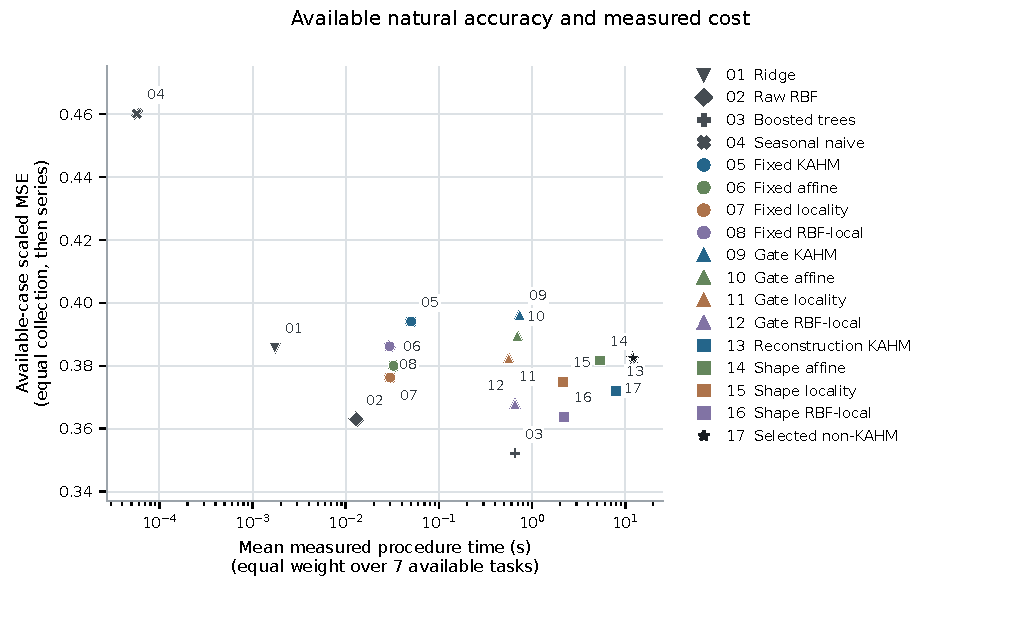
\includegraphics[width=\linewidth]{generated/direct_reconstruction/natural_available_accuracy_cost.pdf}
\caption{Available-case natural accuracy and implemented cost for all
17 procedures. Accuracy averages equally across three collections; time
averages equally across seven feasible task suites, with a logarithmic
horizontal scale. The missing rideshare collection is not replaced.
This descriptive plot does not establish population uncertainty or an
application-specific acceptable-cost threshold.}
\label{fig:direct-natural-cost}
\end{figure}
\FloatBarrier

\FloatBarrier
\section{Online adaptation: protocol and resource measurements}
\label{app:adaptive-development}

\paragraph{Inputs and temporal roles.}
The eight synthetic streams contain 2,048 retained observations each, after
256 regime-A burn-in observations. Four seeds, 20261101--20261104, pair
stationary and recurring schedules by innovations. Histories and horizons
are respectively 12 and $(1,4,12)$. The retained Dominick series T7830,
T25851 and T108533 each contain 393 weekly observations, with histories 52
and horizons $(1,2,4)$. The Sunspot input is the finite final 4,096-point
crop of the previously selected daily T1 series, starting at original raw
index 69,828; histories are 28 and horizons $(1,3,7)$. No interpolation is
used. The source archives and version identifiers are documented with the
reproduction materials \citep{Godahewa2021Monash}.

At observation time $t$, the evaluator scores previously issued forecasts
whose targets mature at $t$, releases the newly available labels, updates
the model, then issues forecasts for $t+h$. Initial fitting uses common
joint-horizon complete rows, and calibration weights are selected before
processing the first evaluation observation using only earlier targets.
Matured earlier evaluation labels may update the model; the update rule and
selected weights remain fixed. The model therefore uses labels from earlier evaluation times once
they become available, while the update algorithm remains fixed. Scale factors use the fitting
prefix only. Losses average origins within horizon, horizons within series,
then series within collection; Dominick and Sunspot receive equal weight.
The four seeds define independent simulation replications; forecasts
from overlapping windows within a stream are dependent. No broad transfer intervals
are claimed from the two selected natural collections.

\paragraph{Reference policy and calibration scope.}
The geometric bank contains four local models of rank at most two. Every
16 observations, an adaptive arm considers one local model in round-robin
order, retains half its initial references as anchors, and replaces at most
four other references with observed histories assigned to that local model.
The affected geometry and all residual heads are rebuilt coherently from
their bounded replay. No bandwidth, penalty, history, reference-policy or
refresh search is performed. The kernel comparator uses an initial-prefix
median-distance bandwidth, regularizer 0.1 and FIFO supports, with recorded
inverse-residual checks and rebuilds. Calibration selects only the four
possible horizon-specific correction weights stated in
Section~\ref{sec:adaptive-development}.
For the kernel comparator, the correction is its kernel forecast minus
the common raw ridge forecast. The same calibration rule therefore selects
a ridge--KRR mixture for each horizon: weights one and zero recover KRR
and ridge, respectively. All reported method losses include this selection.

\paragraph{Prespecified accuracy and service criteria.}
The decision to expand the evaluation requires one capacity setting
to satisfy all accuracy and service criteria. On recurring
streams, adaptive KAHM must reduce mean loss by at least 3\% against each
of adaptive affine, adaptive RBF-local and kernel ridge, with wins on at
least three of four paired seeds against each, and by at least 1\% against
both fixed KAHM and raw ridge. On the natural aggregate, it must improve
each of the three main comparators by at least 1\%; at least one collection must show improvements of at least 3\%
against all three comparators, and neither collection may be more
than 5\% worse than any. KAHM must also meet the per-stream 99th-percentile service-time screen,
with no unexpected exception or cap violation in any method. These
thresholds were fixed before the original run and were also used for
the repeated evaluation after the numerical amendment, designated A1.
Neither capacity setting meets the recurring-stream accuracy criteria.
The protocol therefore classifies both settings as insufficient for
expanding the experiment. Every criterion is evaluated within a single
capacity setting.

% Generated from saved task-level resource measurements.
\begin{table}[!htbp]
\centering\small\setlength{\tabcolsep}{5pt}
\caption{Measured service and state by method/tier. P99 denotes the 99th percentile and is first computed per stream, then maximized across the 12 streams. Other columns also report maxima; they may occur on different streams. Owned NumPy buffers exclude Python objects and temporary work arrays; worker resident set size (RSS) includes interpreter, libraries and evidence storage. Neither is a precise incremental deployment footprint.}
\label{tab:adaptive-development-resources}
\begin{tabular}{@{}llrrrr@{}}
\toprule
Method & Tier & P99 (ms) & Max (ms) & NumPy (KiB) & RSS (MiB) \\
\midrule
Raw ridge & Small & 0.55 & 1.77 & 300.34 & 150.48 \\
Raw ridge & Large & 1.26 & 4.54 & 465.72 & 150.48 \\
Fixed KAHM & Small & 4.98 & 29.01 & 466.29 & 150.48 \\
Fixed KAHM & Large & 8.61 & 27.24 & 685.38 & 150.48 \\
Adaptive KAHM & Small & 9.89 & 49.10 & 518.95 & 150.48 \\
Adaptive KAHM & Large & 11.75 & 23.60 & 824.52 & 150.48 \\
Adaptive affine & Small & 9.56 & 24.75 & 509.83 & 150.48 \\
Adaptive affine & Large & 7.00 & 13.44 & 791.39 & 150.48 \\
Adaptive RBF-local & Small & 5.05 & 12.05 & 509.83 & 150.48 \\
Adaptive RBF-local & Large & 4.58 & 8.00 & 791.39 & 150.48 \\
Sliding-window KRR & Small & 3.15 & 3.95 & 477.34 & 150.48 \\
Sliding-window KRR & Large & 3.42 & 13.49 & 1011.72 & 150.48 \\
\bottomrule
\end{tabular}
\end{table}


\paragraph{Resource scope.}
Workers execute serially in fresh processes with one numerical thread and
the same CPU affinity. Initialization and calibration are measured
separately. The service interval covers history/pair assembly, all matured
horizon updates, feature/head rebuilds, kernel inverse audits and prediction;
scoring, serialization and state inspection are excluded. Buffer-state
samples and whole-worker peak RSS have the distinct scopes stated in
Table~\ref{tab:adaptive-development-resources}. The 20\,ms allowance is a
host-specific engineering screen, not an application-derived service-level
requirement. Different support sharing across horizons prevents interpreting
the tier labels as equal memory or equal computation.

\paragraph{Solver amendment and computational verification.}
The original implementation accumulated correction cross-products;
large rows entering and leaving a finite window produced cancellation in
the reproduced failing state. The amended implementation (A1) recomputes residuals against the
current baseline from the same bounded replay, centers to eliminate the
free intercept, equilibrates both data and penalty columns, and solves
the augmented ridge objective with pivoted QR. It changes arithmetic, not
the specified objective or advancement rule. The original 144 runs remain
in \path{extensions/adaptive_development/archives/initial_attempt.zip}.
Because the amended runs repeat the same inputs, they do not increase
the number of independent experimental replications. The verification program passes
\ADAuditChecks{} computational consistency checks, covering chronology,
coverage, calibration selection, aggregation, decision gates, resources,
shared baselines and matched reference changes. It imports neither the
forecasting model nor its analyzer, but remains an internal computational
check rather than independent scientific replication.

The reproduction materials contain both versions of the protocol and
source, the numerical diagnostic states, input hashes, predictions,
update traces, and summaries. The manuscript builder
\path{extensions/tmlr_integration/build_adaptive_assets.py} reconstructs
the displayed collection means and resource maxima from saved task
records, checks them against the analysis and decision files, and records
input/output hashes. It performs no model fitting. Both execution checkpoints were recorded locally. The study was not
publicly preregistered.

\FloatBarrier
\section{Shared follow-up protocol, inference, and evidence generation}
\label{app:followup-protocols}

\subsection{Data and independent units}

Both follow-ups retain the declared \texttt{linear\_ar},
\texttt{nonlinear\_ar}, Van der Pol, and Duffing observation laws and
their inherited integration, initial-condition, burn-in, and observation
rules. Each has \PPRepetitions\ repetition units and added-noise levels
$0$ and $0.1$, hence \PPTasks\ tasks. Episode length is seventy-two,
history width \PPHistory, horizons $1,4,12$, and origin stride four.
A/B/C/D allocate \PPEpisodesA/\PPEpisodesB/\PPEpisodesC/\PPEpisodesD\
underlying episodes, retaining \PPRowsA/\PPRowsB/\PPRowsC/\PPRowsD\
histories. The \PPOrigins\ origins of one episode are dependent.
Added noise is the prescribed level times the population standard
deviation of unaugmented A episode values times a unit Gaussian draw;
both histories and targets are augmented.

Underlying generation, unit-noise, row-retention, and fit streams are
paired across competitors and noise levels. The preprocessing study uses
master seed \texttt{2026110117}; the residual study uses
\texttt{2026110173}. Integer-component NumPy \texttt{SeedSequence}
derivation and prior-stream exclusion checks are frozen in each
configuration. The latter seed is replayed in the computational
reproduction. Distinct seeds across the two scientific designs do not
turn a repeat execution of one seed roster into additional observations.
All prescribed tasks are required, and unexpected failures stop execution
rather than removing or replacing difficult tasks.

\subsection{Native geometry and decoder grids}

Each transformed-history bank requests partitions with $2,4,8$ local
groups, using at most twenty-four references per group and the retained
fitting histories. For cap $c$, ambient dimension $d$, and $n_j$ local
references, initialize $r_j=\min\{c,d,n_j-1\}$. Retain covariance
eigenvalues above double-precision epsilon. If the smallest range of a
projected reference coordinate is below $10^{-3}$, reduce the requested
rank and recompute until the range condition holds or requested rank one
is reached. The explicit zero-admissible-rank case remains a rank-zero
wrapper. No extra $d-1$ restriction is imposed.

Let $Q_j$ contain transformed references, $P_j$ the local basis, and
$S_j$ their projected sample covariance. At positive rank, the shared
Gaussian kernel is
\[
 \kappa_j(z,z')=
 \exp\!\left[-\frac{(P_j^\top(z-z'))^\top S_j^{-1}
                         P_j^\top(z-z')}{2r_j}\right].
\]
With Gram matrix $K_j$, query vector $k_j$, and reference-fitted positive
regularizer $\lambda_j$, set $C_j=(K_j+\lambda_jI)^{-1}$.
The KAHM and positive-kernel reconstructions are respectively
$Q_j^\top C_j k_j/(\mathbf1^\top C_jk_j)$ and
$Q_j^\top k_j/(\mathbf1^\top k_j)$; the affine reference is
$\mu_j+P_jP_j^\top(z-\mu_j)$.
The reference-only regularizer retains the inherited reconstruction
iteration; it is never selected from forecast targets.

Within each partition, locality gates are normalized exponentials of
negative squared distance to the local centers, divided by twice their
fitted squared-radius scales. The common block stacks each gate and its
gate-weighted principal coordinates. A departure block stacks the
gate-weighted difference between a nonlinear reconstruction and the
affine reconstruction, retaining all ambient coordinates. Within a fixed
bank, KAHM and RBF share references, projected kernels, gates, and width.
Independent scaler/cap selection may choose different banks.

Column standardization uses the designated fitting feature rows. For a
standardized block $u\in\R^p$, the radial map is
$u/\sqrt{1+\|u\|_2^2/p}$, with zero mapped to zero.
Complete bounded heads concatenate separately bounded common and
departure blocks. Fixed-common heads use only a bounded departure block,
center it on their fitting rows, fit centered residual slopes, and omit
the response-mean intercept. Their correction bound uses
$\sqrt p+\|\bar\varphi\|_2$ after centering; a bound on that correction
does not bound the common forecast or certify small prediction error.

Query kernels use a common log shift before exponentiation. A signed
normalization ratio at most $10^{-10}$, or an undefined/nonfinite required
quantity, invokes the documented affine reconstruction fallback, making
that raw local departure zero. Feature standardization follows this
operation, so a zero raw departure need not remain zero after centering.
Unexpected factorization, coordinate, gate, or kernel failures stop the
study and are distinct from declared local guards.

\begin{table}[t]
\centering\small
\caption{Frozen grids shared by the two follow-ups, except that the
new cross-fit/fold/half-training searches omit the redundant cap twenty.
Raw RBF receives three history scalers; geometric complete procedures
receive the five declared common/departure pairs. These grids do not
assert equal computation or representation width.}
\label{tab:supp-followup-grids}
\begin{tabular}{@{}p{0.43\linewidth}p{0.51\linewidth}@{}}
\toprule
Setting & Frozen value \\
\midrule
Ridge penalties, each horizon & $\{0.0001,0.001,0.01,0.1,1\}$ \\
Calibration multipliers, each horizon & $\{0,0.25,0.5,1\}$ \\
Preprocessing-study native caps & $\{1,2,4,8,12,20\}$ \\
Requested partition counts & $\{2,4,8\}$ \\
References per local model / bank rows & At most 24 / 512 \\
Raw RBF landmark count & At most 64 \\
Raw RBF bandwidth factors & $\{0.5,1,2\}$ \\
HGB learning rates / leaf counts & $\{0.05,0.1\}$ / $\{7,15\}$ \\
HGB iterations / L2 penalty & 100 / 1 \\
Feature-scale / target-variance floors & $10^{-6}$ / $10^{-12}$ \\
\bottomrule
\end{tabular}

\end{table}

Raw Nystr\"om RBF concatenates its landmark features with the transformed
raw history, then standardizes columns and fits ridge. Its bandwidth
factors multiply the inherited positive-median squared-distance rule;
zero positive-distance support uses the declared unit fallback. Boosting
has no early stopping. Persistence uses the latest observed history value.
Every fit, history transform, feature normalization, and search depends
only on its declared fitting/development inputs. C calibrates frozen
procedures; D supplies fixed-state forecasts and final evaluation only.

\subsection{Loss, primary margins, and secondary uncertainty}
\label{app:followup-inference}

For task $t$, horizon $h$, and procedure $m$, define
\begin{equation}
 L_{t,h,m}=\frac{n_D^{-1}\sum_{i\in D}
                   (y_{ih}-\widehat f_{m,h}(x_i))^2}
                   {\max\{\operatorname{Var}_A(Y_h),10^{-12}\}}.
 \label{eq:supp-followup-smse}
\end{equation}
The denominator is the retained full-A target population variance for
every evaluated method, including P/R and half-training controls. It
does not change the subset-only normalizers used for common-model fitting
and B selection. Average horizons equally, then laws and noise levels
equally within each repetition. The nonlinear panel has eighteen
law/noise/horizon cells per repetition; the linear control has six.
Point gain is $100(1-\bar L_c/\bar L_m)$, a ratio of mean repetition
losses rather than an average of cell percentage gains.

Each follow-up retains its own original four-claim primary family.
For nonlinear superiority the repetition margin gap is
$d_r=0.97L_{r,m}-L_{r,c}$; linear noninferiority uses
$d_r=1.05L_{r,\mathrm{ridge}}-L_{r,c}$.
With $n=24$, family level $0.05$, and four comparisons, the lower endpoint is
\begin{equation}
 \bar d-t_{1-0.05/4,\,23}\frac{s_d}{\sqrt{24}}.
 \label{eq:supp-followup-primary-bound}
\end{equation}
Only a strictly positive endpoint establishes the stated claim.
These are approximate repetition-level paired-$t$ calculations, without
distribution-free coverage guarantees. The two later families are not
pooled with each other or with the principal dimension experiment's six
claims. In the computational reproduction, the calculations refer to the
same original repetition units, whose outputs had previously been reported.

Secondary contrasts use ordinary two-sided 95\% paired-$t$ intervals over
the repetition aggregates, explicitly labeled descriptive and unadjusted.
They do not select a new primary candidate after D is observed. The
in-sample KAHM/expanded-policy ratio is shown as a point description only;
no new interval or test is introduced for that comparison. Neither tasks,
horizons, folds, nor overlapping origins are treated as extra independent
replications. Stability screens and norm-bound diagnostics remain separate
from predictive margin decisions.

\subsection{Frozen evidence and reproducible displays}

Source, fits, predictions, and target release have separate recorded
identities. The preprocessing study freezes its source before production
generation. The reproduction has new phase seals around regenerated data
and recomputed states; they describe only that execution. Procedural
masking and hash checks do not supply cryptographic access isolation or
authenticate missing historical records.

The manuscript's \path{build_followup_assets.py} reads the existing
analysis tables, source freezes, phase seals, and passing independent audit
receipts. It checks displayed-table hashes against the hash-bound analysis
summary and checks the audit's summary, source, and seal identities.
It generates the two \path{generated/preprocessing_dimension/} and
\path{generated/crossfit_residual/} namespaces. Their
\path{metrics.json} files retain unrounded values, meanings, and rounding
for every prose macro; their \path{asset_manifest.json} files identify
input and output SHA-256 hashes. Manuscript compilation uses the generated
files and requires no raw scientific arrays. Regeneration requires the
study evidence and performs no fitting, reselection, new scoring, or new
hypothesis tests. Its consistency checks do not replace either production
audit.

The original cross-fit protocol, numerical amendment, and pinned source
manifest are preserved in the reproduction package. The corrected
production verifier and its regression receipts are separate from the
frozen scientific prediction implementation. Neither a repaired verifier
nor a successfully reproduced aggregate establishes the authenticity of
the unavailable original completed execution. The empirical scope remains
the declared synthetic laws, finite samples, history length, horizons, and
selection grids.


\FloatBarrier
\section{Policy-augmentation specifications and reproducibility}
\label{app:policy-augmentation}

This appendix gives the construction, chronology, selection diagnostics,
and computational scope for Section~\ref{sec:policy-augmentation-supp}.
The source and statistical family are separate from those of the
dimension, preprocessing, and reproduced residual-target studies.

\subsection{Construction and complete tuning grids}

History transformations are A-fitted standardization, unclipped min--max
scaling, and $\tanh$ of standardized histories with multiplier one.
Tanh histories receive no subsequent history standardization; feature
scaling and radial bounding remain distinct later operations. Common
and departure maps fit their reference geometry and all feature
statistics using A. The bank uses partitions of sizes $2,4,8$, at most
twenty-four references per local model, and at most $512$ bank-fitting
rows. The feature scale floor is $10^{-6}$ and the inherited relative
normalizer guard is $10^{-10}$.

For requested cap $c$, ambient dimension $d$, and local reference count
$n_j$, native initialization is
\begin{equation}
 r_j^{\mathrm{init}}=\min\{c,d,n_j-1\}.
 \label{eq:supp-pa-rank}
\end{equation}
The existing positive-variance and projected-range rules can reduce the
realized rank. No additional normal direction is reserved. New local
corrections search caps $1,2,4,8,12$ independently for KAHM and RBF.
The inherited complete search retains cap twenty, which duplicates cap
twelve at $d=12$; its tie order favors twelve. Neither requested cap
nor feature width is identified with realized local rank.

\begin{table}[t]
\centering\small
\caption{Frozen parameter grids. B selects penalties separately by
horizon and then one map by mean normalized horizon loss. Existing
complete procedures and new residual corrections retain their stated
calibration targets.}
\label{supp:pa-grids}
\begin{tabular}{@{}p{0.26\linewidth}p{0.68\linewidth}@{}}
\toprule
Component & Candidate values and fitting role \\
\midrule
History maps & Standard, min--max, $\tanh(z)$; fit A, select B. \\
New local corrections & Caps $\{1,2,4,8,12\}$ crossed with the three maps. \\
Inherited geometry & Caps $\{1,2,4,8,12,20\}$; common/departure pairs
$(s,s),(m,m),(t,t),(t,m),(m,t)$, where $s,m,t$ denote standard,
min--max, and $\tanh(z)$. \\
Ridge penalties & $\{10^{-4},10^{-3},10^{-2},10^{-1},1\}$; B by horizon. \\
Calibration & $\{0,\tfrac14,\tfrac12,1\}$; C by horizon. Legacy blends
toward raw ridge; new residual heads toward common plus bias. \\
Complete raw RBF & $64$ A landmarks; bandwidth factors
$\{0.5,1,2\}$; three history maps. \\
Extra raw-RBF residual & $64$ A landmarks; bandwidth factors
$\{0.25,0.5,1,2,4\}$; three history maps. \\
Histogram boosting & Learning rates $\{0.05,0.1\}$, maximum leaves
$\{7,15\}$, $100$ iterations, L2 penalty $1$. \\
\bottomrule
\end{tabular}
\end{table}

Bandwidth factors multiply the median squared landmark distance.
Each new family has fifteen map configurations, seventy-five B scores
per horizon, four C multiplier choices per horizon, and one additional
C family slot. The independently selected KAHM and local-RBF corrections
have width $168$ in the retained fits. Extra raw-RBF residual designs
include the raw history and retained Nystr\"om directions, giving widths
$66$--$76$ in simulation and $59$--$76$ on natural series. Matching the
score counts therefore does not match width or function class.

\subsection{Simulation allocation and diagnostics}

Master seed $2026110191$ defines twenty-four repetitions. The $1,272$
intended-distinct streams were checked against one another and prior
study exclusions, including the complete earlier cross-fit cohort.
Each task has $64/32/32/128$ episodes in A/B/C/D and retained row caps
$512/256/256$ for A/B/C. D retains thirteen origins from each of its
$128$ episodes, giving $1,664$ rows. Episode independence separates
the four roles; overlap among origins within an episode does not create
new inferential units. All fits were sealed before D generation and
all forecasts before D target release. The protocol required execution to halt on unexpected failures rather
than replacing tasks or changing menus.

\begin{table}[t]
\centering\small
\caption{Simulation law/noise summaries. Every condition is retained;
these means and C-selection frequencies are descriptive, with no
additional superiority test or selection of a favorable target population.}
\label{supp:pa-conditions}
% Generated by build_policy_assets.py; do not edit.
\begin{tabular}{@{}lrrrrrr@{}}
\toprule
Law & Noise & $P_0$ & $P_1$ & $P_0^+$ & Gain (\%) & KAHM chosen \\
\midrule
Linear AR & 0.0 & 0.912592 & 0.912592 & 0.912466 & +0.00 & 0/24 \\
Linear AR & 0.1 & 0.915222 & 0.915251 & 0.915407 & -0.00 & 1/24 \\
Nonlinear AR & 0.0 & 0.019451 & 0.019463 & 0.019451 & -0.06 & 5/24 \\
Nonlinear AR & 0.1 & 0.031684 & 0.031687 & 0.031684 & -0.01 & 6/24 \\
Van der Pol & 0.0 & 0.004096 & 0.004012 & 0.004096 & +2.05 & 2/24 \\
Van der Pol & 0.1 & 0.053886 & 0.052955 & 0.053651 & +1.73 & 14/24 \\
Duffing & 0.0 & 0.011021 & 0.010874 & 0.011009 & +1.34 & 11/24 \\
Duffing & 0.1 & 0.043474 & 0.043284 & 0.043460 & +0.44 & 5/24 \\
\bottomrule
\end{tabular}

\end{table}

\begin{table}[t]
\centering\small
\caption{B-selected requested caps and transformations. Counts refer to
candidate fits, including tasks on which C ultimately rejects KAHM.
They neither rank transformations using D nor identify a universal
preferred dimension.}
\label{supp:pa-selections}
% Generated by build_policy_assets.py; do not edit.
\begin{tabular}{@{}lrrrrrrrr@{}}
\toprule
KAHM cohort & 1 & 2 & 4 & 8 & 12 & Standard & Min--max & Tanh \\
\midrule
Simulation (192) & 44 & 71 & 45 & 24 & 8 & 65 & 93 & 34 \\
Natural (48) & 12 & 10 & 15 & 5 & 6 & 12 & 16 & 20 \\
\bottomrule
\end{tabular}

\end{table}

The $2,688$ selected KAHM local-model occurrences in simulation have
realized ranks from zero to twelve, including five admissible zero-rank
bases. The $672$ natural occurrences have ranks from one to twelve and
no zero-rank basis. Bank occurrences are not independent observations.
The inherited solver attempts its original ridge SVD and uses a logged
alternative driver only after the declared linear-algebra exception.
Simulation records contain one successful recovery and no unrecovered
failure; natural fitting contains neither a recovery nor a failed task.
Numerical recovery and native rank reduction are different events.

\subsection{Natural roster, chronological windows, and loss scales}

The pinned M4 Train snapshot contains $359$ Weekly and $414$ Hourly
series. Length eligibility requires $N\geq475$; $258$ Weekly series
qualify. The full list of seventy-two prior pilot identities is
excluded; twenty-four are Hourly, leaving $390$ eligible Hourly series.
Within each frequency, the protocol sorts SHA-256 hashes of
\texttt{kahm-policy-augmentation-natural-2026-11-01-v1|Frequency|ID}
and selects the first twenty-four. Observation magnitudes, validation
errors, and model success never enter this rule. The complete retained
roster appears in Table~\ref{supp:pa-roster}.

\begin{table}[t]
\centering\small
\caption{Complete natural-series roster from the fixed identity-hash
rule. These forty-eight anonymous identities are benchmark units, not
asserted independent application sources.}
\label{supp:pa-roster}
% Generated by build_policy_assets.py; do not edit.
\begin{tabular}{@{}lrrlrr@{}}
\toprule
Weekly ID & $N$ & A rows & Hourly ID & $N$ & A rows \\
\midrule
W160 & 1644 & 512 & H216 & 960 & 512 \\
W43 & 1017 & 512 & H325 & 960 & 512 \\
W114 & 1044 & 512 & H299 & 960 & 512 \\
W39 & 1512 & 512 & H368 & 960 & 512 \\
W293 & 1207 & 512 & H53 & 700 & 481 \\
W170 & 1644 & 512 & H220 & 960 & 512 \\
W196 & 824 & 512 & H300 & 960 & 512 \\
W32 & 1603 & 512 & H343 & 960 & 512 \\
W38 & 510 & 291 & H128 & 700 & 481 \\
W164 & 1644 & 512 & H11 & 700 & 481 \\
W66 & 2178 & 512 & H252 & 960 & 512 \\
W287 & 934 & 512 & H21 & 700 & 481 \\
W252 & 2178 & 512 & H164 & 700 & 481 \\
W82 & 1351 & 512 & H255 & 960 & 512 \\
W3 & 2178 & 512 & H402 & 960 & 512 \\
W142 & 849 & 512 & H28 & 700 & 481 \\
W48 & 1293 & 512 & H211 & 960 & 512 \\
W146 & 1644 & 512 & H282 & 960 & 512 \\
W247 & 1603 & 512 & H76 & 700 & 481 \\
W238 & 1602 & 512 & H148 & 700 & 481 \\
W125 & 2283 & 512 & H175 & 960 & 512 \\
W289 & 1087 & 512 & H380 & 960 & 512 \\
W232 & 1602 & 512 & H166 & 700 & 481 \\
W206 & 934 & 512 & H356 & 960 & 512 \\
\bottomrule
\end{tabular}

\end{table}

At origin $t$, the history is $(y_{t-11},\ldots,y_t)$ and targets are
$y_{t+h}$ for $h\in\{1,4,12\}$. D contains the final thirty-two
eligible origins. Moving backwards gives sixty-four C and sixty-four
B origins, with twelve intervening origins omitted at each boundary.
A contains $\min(512,N-219)$ preceding origins, also separated from B
by twelve omitted origins. The largest target index of an earlier
block precedes the next block's first origin, so targets do not overlap
between blocks. Within-block histories and origins remain dependent.
The realized A size is $291$ for W38, $481$ for selected length-$700$
Hourly series, and $512$ for the other selected series. No parameter
is refitted after C. Later D histories can include earlier D outcomes
already observed at the current origin.

Seasonal naive accesses the latest available observation at the same
seasonal position, using lag $52$ Weekly and $24$ Hourly. The Weekly
lag is a declared annual control, not the official M4 Weekly Naive2
convention. Drift uses the earliest observation entering an A history
and the current observation. Both controls are causal at each origin.
The complete natural-policy tie order is the seven inherited non-KAHM
families, shared-bias common, in-sample RBF, seasonal naive, drift, and
finally the relevant added family.

SMSE uses the horizon-specific A-target population variance with floor
$10^{-12}$. Secondary seasonal MASE uses an A-only raw-prefix mean
absolute seasonal difference at lags $52/24$; frequency MASE uses
lags $1/24$. The prefix extends from the first observation in an A
history through the last A target. Both denominator floors are
$10^{-12}$ and neither activates. Overall seasonal MASE for
$(P_0,P_1,P_0^+)$ is $(0.626066,0.630946,0.629528)$; frequency MASE is
$(1.380930,1.390215,1.404932)$. These are descriptive,
study-specific repeated-origin scores.

\subsection{Source identity, computation, and verification scope}

The combined scientific source is commit
\texttt{b1915813e98a59572a4bbb800adc2bd1f3fccc1b}; the subsequent
results release is
\texttt{b59410407a7cd34155aa1955fe0c801f62381364}.
The M4 input snapshot is
\texttt{6c1067e5a57161249b17289a565178dc7a3fb3ca}.
The simulation extension is \path{extensions/policy_augmentation_20261101}
and the natural extension is
\path{extensions/policy_augmentation_natural_20261101}.
Each retains its own protocol, source/configuration freeze, fit and
prediction seals, target-release record, analysis, and audit receipt.

The simulation local freeze preceded new A/B/C/D generation and its
source was published before terminal D generation. The natural source
was frozen locally before numerical parsing and published after its
evaluation. Raw public Train bytes remained available throughout;
staged parsing and target masking document execution order without
providing cryptographic access isolation. Neither design is a public
preregistration. Earlier method-development outcomes were known, and
the new simulation laws were not unseen application domains.

\begin{table}[t]
\centering\small
\caption{Recorded whole-suite resources, including rejected and
diagnostic candidates. Worker times sum concurrent work; peak RSS is
the largest individual worker measurement. Complete compressed fitting
records are not minimal deployed-model sizes.}
\label{supp:pa-resources}
% Generated by build_policy_assets.py; do not edit.
\begin{tabular}{@{}lrr@{}}
\toprule
Whole-suite measurement & Simulation & Natural \\
\midrule
Fit-worker wall seconds, summed & 2,723.65 & 382.68 \\
Fit-worker CPU seconds, summed & 2,718.92 & 381.13 \\
Largest worker RSS (MiB) & 301.09 & 238.59 \\
Complete compressed fitted states (MiB) & 1,808.99 & 186.87 \\
\bottomrule
\end{tabular}

\end{table}

Three fresh workers execute tasks with one numerical thread each.
Summed worker durations are distinct from stage elapsed time, and the
largest worker RSS is not aggregate concurrent memory. Shared fits
prevent interpreting whole-suite costs as isolated marginal costs of
$P_0$ or $P_1$; the extra-family timing excludes its shared common
predictor.

The synthetic saved-record audit passes for all $192$ tasks, $9,600$
forecast arrays, and $5,376$ selected local bases. It reconstructs every
retained terminal loss and all four primary bounds, checks seed
exclusions and B/C decisions, verifies exact policy forwarding, and
independently solves selected extra-RBF ridge coefficients. The natural
audit covers all $48$ series, $2,016$ forecast arrays, $10,800$ B
penalty paths, $576$ C multiplier decisions, $144$ policy decisions,
and $576$ selected ridge normal equations, including raw-source
indexing and causal direct controls. Both audits reuse inherited feature
maps; they do not independently reimplement every KAHM map or refit
every unselected candidate. Their successful checks establish
consistency of the retained computation, not external scientific
replication, forecast accuracy, or a distribution-free risk guarantee.

\FloatBarrier
\end{document}
